\documentclass[10pt]{article}
\usepackage[utf8]{inputenc}
\usepackage[T1]{fontenc}
\usepackage{amsmath}
\usepackage{amsfonts}
\usepackage{amssymb}
\usepackage[version=4]{mhchem}
\usepackage{stmaryrd}
\usepackage{graphicx}
\usepackage[export]{adjustbox}
\graphicspath{ {./images/} }
\usepackage{caption}
\usepackage{bbold}

\DeclareUnicodeCharacter{2234}{\ifmmode\therefore\else{$\therefore$}\fi}
\DeclareUnicodeCharacter{2713}{\ifmmode\checkmark\else{$\checkmark$}\fi}

\begin{document}
\captionsetup{singlelinecheck=false}
Gina correctly started to answer the following question. Complete her solution.\\
Question: Solve the following equation for all real values of $\theta$.\\
Express your answer in radians correct to 3 decimal places.

$$
3 \sin ^{2} \theta-14 \sin \theta-5=0
$$

Gina's solution: $3 \sin ^{2} \theta-14 \sin \theta-5=0$

$$
(3 \sin \theta+1)(\sin \theta-5)=0
$$

Find and simplify the 6th term in the binomial expansion of $\left(3 x^{4}-\frac{1}{x^{3}}\right)^{9}$.

The number of times a website is visited can be modeled by the function:

$$
A=800(e)^{r t}
$$

where $A=$ the total number of visitors at time $t$

$$
t=\text { the time in days }(t \geq 0)
$$

$r=$ the rate of growth\\
After 5 days, 40000 people have visited the site.\\
Determine the number of visitors expected after 9 days.\\
Express your answer as a whole number.

Solve algebraically:

$$
10^{3 x}=7^{x+5}
$$

Express your answer correct to 3 decimal places.

A word contains two Ms, two Es, two Ns, and no other repeated letters.\\
Suppose one of the Ns is replaced by an M.\\
Will this replacement result in greater or fewer permutations?\\
Justify your reasoning.

There is a group of 16 boys and 12 girls. How many ways can a committee of 3 people be formed if there must be at least 2 girls on the committee?\\
Express your answer as a whole number.

\begin{verbatim}
Note: A calculator is not required for the remaining test questions.
\end{verbatim}

A student is using the formula $s=\theta r$ to find an arc length of a circle. Given a central angle measure of $35^{\circ}$ and a radius of 6 cm , the student's solution is as follows:

$$
\begin{aligned}
& s=(35)(6) \\
& s=210 \mathrm{~cm}
\end{aligned}
$$

Explain why this solution is incorrect.\\
Write the correct solution.

Given the graph of $f(x)$ below, explain how you would sketch the graph of $y=|f(x)|$.\\
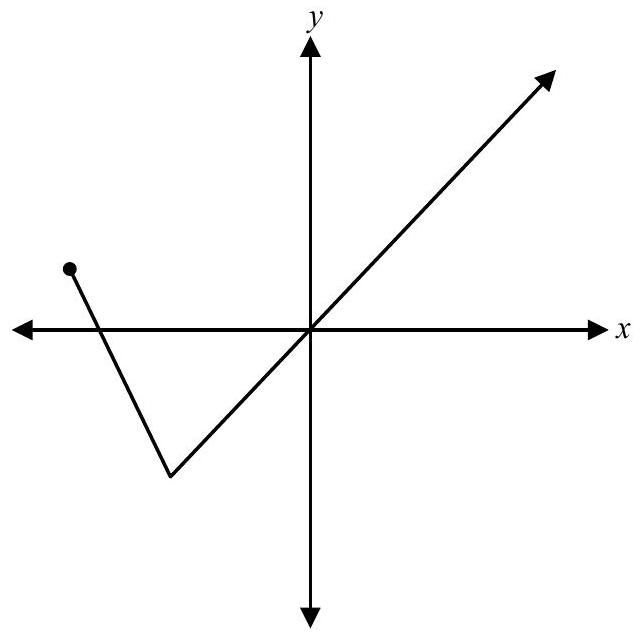
\includegraphics[max width=\textwidth, alt={}, center]{de5fb11a-28c7-4ac7-b7ff-0309cebac724-007_637_641_1714_279}

Claire correctly solves the following equation:

$$
\log _{2}(6-x)+\log _{2}(3-x)=2
$$

She finds two possible values of $x: x=2$ and $x=7$.\\
Identify which one of these values is unacceptable and explain why.

Given the graph of the function $f(x)$ below, state the domain of $y=\sqrt{f(x)}$.\\
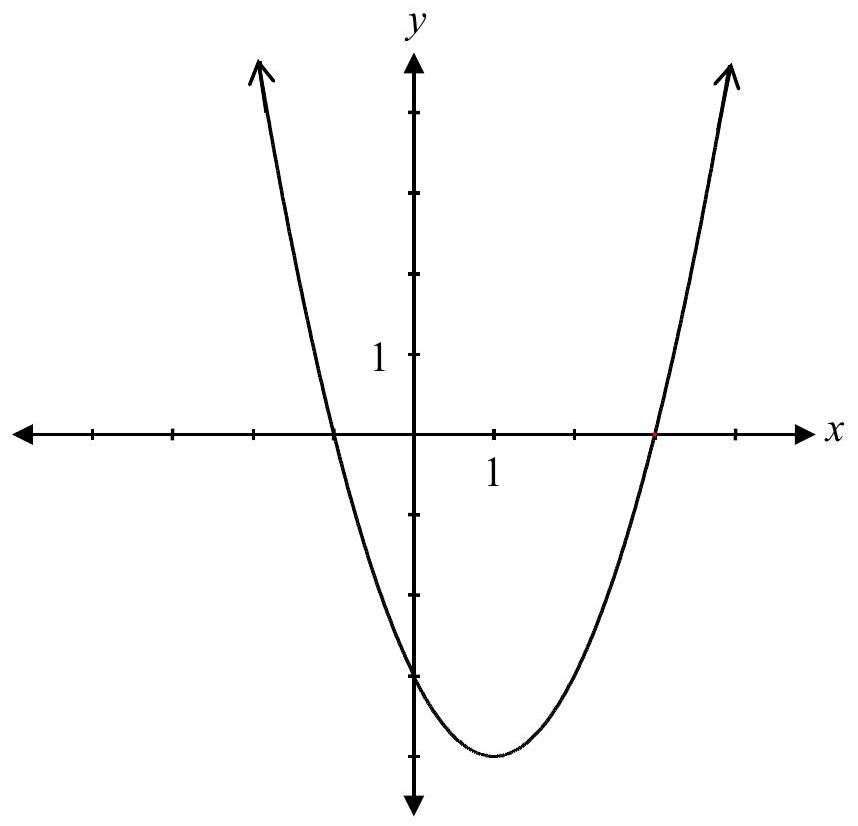
\includegraphics[max width=\textwidth, alt={}, center]{de5fb11a-28c7-4ac7-b7ff-0309cebac724-008_826_858_1673_296}

A school offers 4 different Science courses, 3 different Mathematics courses, and 2 different English courses.\\
Julie must select 1 Science course, 1 Mathematics course, and 1 English course. She thinks this creates 9 options for her timetable.\\
Show why Julie is incorrect.

\section*{Question 12}
Explain how Pascal's triangle can be used to determine the coefficients in the binomial expansion of $(x+y)^{n}$.

Prove the identity below for all permissible values of $x$ :

$$
\frac{1+\cos 2 x}{\sin 2 x}=\cot x
$$

\begin{center}
\begin{tabular}{|l|l|}
\hline
Left-Hand Side & Right-Hand Side \\
\hline
 &  \\
\hline
\end{tabular}
\end{center}

Your classmate, Leo, was absent for one of his math lessons.\\
Explain to Leo how to determine the cosecant ratio for an angle in standard position given that $\mathrm{P}(-3,-4)$ is a point on the terminal arm of the angle.

Given the following graphs:

$$
f(x)
$$

\begin{center}
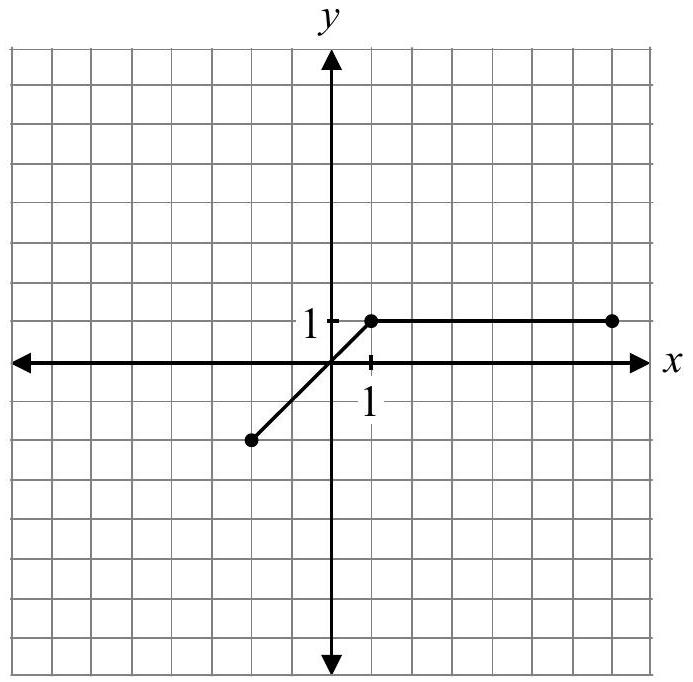
\includegraphics[max width=\textwidth, alt={}]{de5fb11a-28c7-4ac7-b7ff-0309cebac724-012_682_693_528_300}
\end{center}

$$
g(x)
$$

\begin{center}
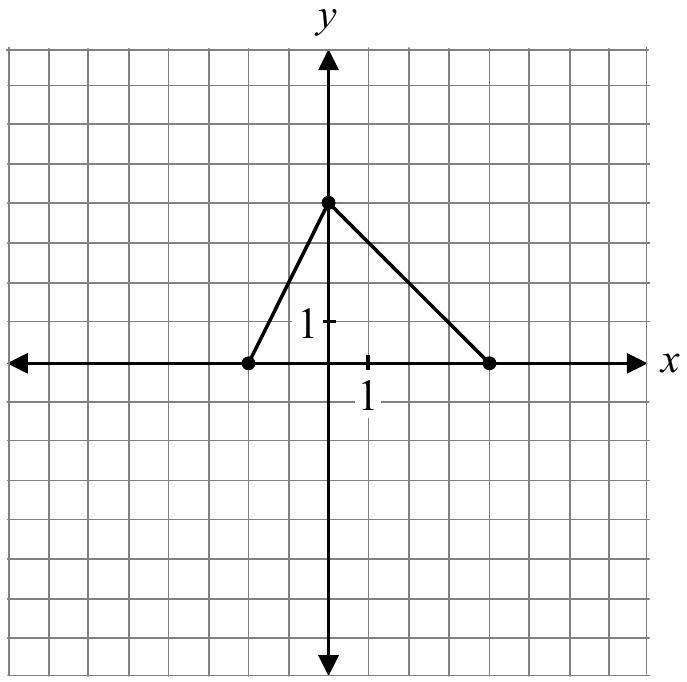
\includegraphics[max width=\textwidth, alt={}]{de5fb11a-28c7-4ac7-b7ff-0309cebac724-012_682_687_528_1168}
\end{center}

Sketch the graph of $f(x)+g(x)$.\\
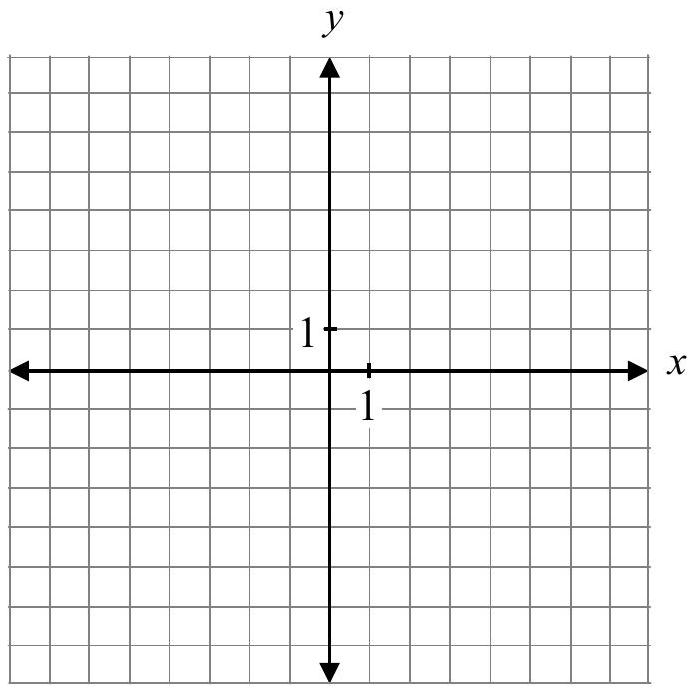
\includegraphics[max width=\textwidth, alt={}, center]{de5fb11a-28c7-4ac7-b7ff-0309cebac724-012_691_693_1473_689}

If $(2,3)$ is a point on the graph of $y=f(x)$, what point must be on the graph of $y=3 f\left(\frac{1}{4} x\right)$ ?\\
a) $\left(\frac{1}{2}, 1\right)$\\
b) $\left(\frac{1}{2}, 9\right)$\\
c) $(8,1)$\\
d) $(8,9)$

Question 17

Consider the arc drawn on each circle. Which arc measure is closest to 3 radians?

\begin{figure}[h]
\begin{center}
\captionsetup{labelformat=empty}
\caption{a)}
  
\includegraphics[alt={},max width=\textwidth]{de5fb11a-28c7-4ac7-b7ff-0309cebac724-013_197_212_1310_298}
\end{center}
\end{figure}

\begin{figure}[h]
\begin{center}
\captionsetup{labelformat=empty}
\caption{b)}
  
\includegraphics[alt={},max width=\textwidth]{de5fb11a-28c7-4ac7-b7ff-0309cebac724-013_130_132_1344_760}
\end{center}
\end{figure}

\begin{figure}[h]
\begin{center}
\captionsetup{labelformat=empty}
\caption{c)}
  
\includegraphics[alt={},max width=\textwidth]{de5fb11a-28c7-4ac7-b7ff-0309cebac724-013_229_238_1295_1196}
\end{center}
\end{figure}

\begin{figure}[h]
\begin{center}
\captionsetup{labelformat=empty}
\caption{d)}
  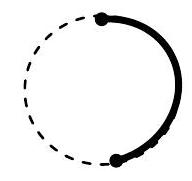
\includegraphics[alt={},max width=\textwidth]{de5fb11a-28c7-4ac7-b7ff-0309cebac724-013_181_192_1319_1611}
\end{center}
\end{figure}

\section*{Question 18}
If $\log _{2} x=4$, then $\log _{2}(2 x)$ is equal to:\\
a) 5\\
b) 8\\
c) 16\\
d) 32

Simplify the following expression:

$$
\cos ^{2} x\left(1+\cot ^{2} x\right)
$$

a) $\sin ^{2} x$\\
b) $\cos ^{2} x$\\
c) $\cot ^{2} x$\\
d) $\sec ^{2} x$

\section*{Question 20}
Identify the graph of the function $y=\frac{x}{x}$.\\
a)\\
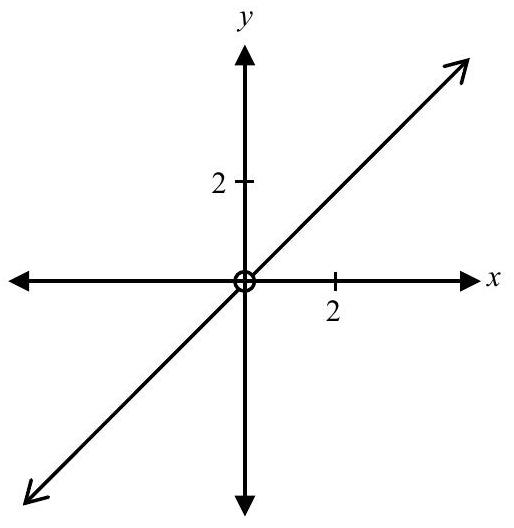
\includegraphics[max width=\textwidth, alt={}, center]{de5fb11a-28c7-4ac7-b7ff-0309cebac724-014_528_514_1370_382}\\
b)\\
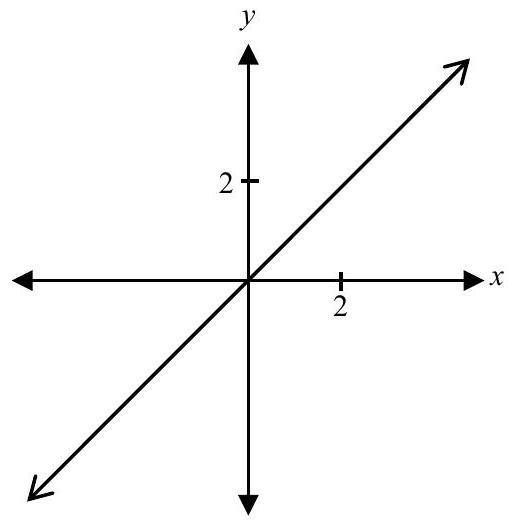
\includegraphics[max width=\textwidth, alt={}, center]{de5fb11a-28c7-4ac7-b7ff-0309cebac724-014_525_523_1312_1228}\\
c)\\
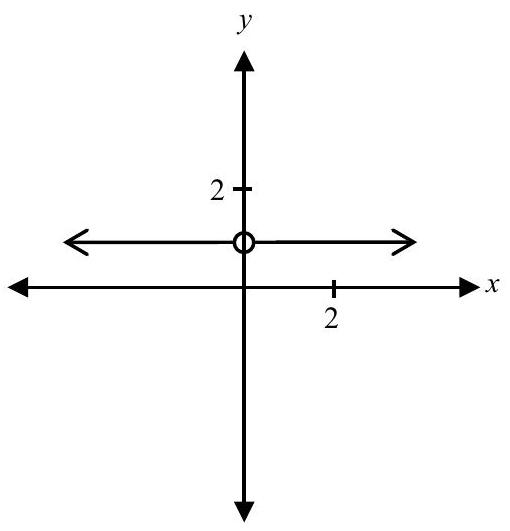
\includegraphics[max width=\textwidth, alt={}, center]{de5fb11a-28c7-4ac7-b7ff-0309cebac724-014_531_510_1987_382}\\
d)\\
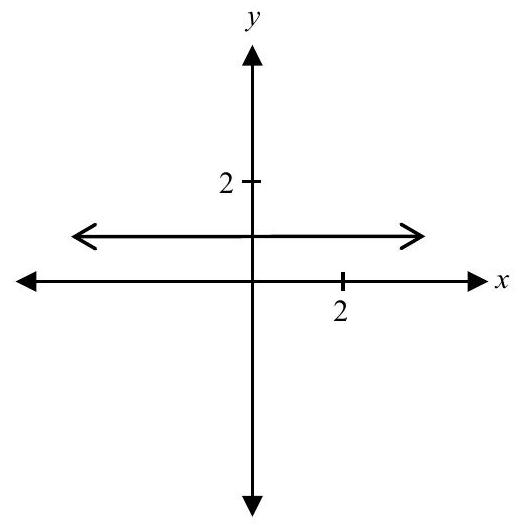
\includegraphics[max width=\textwidth, alt={}, center]{de5fb11a-28c7-4ac7-b7ff-0309cebac724-014_525_519_1972_1237}

How many terms are in the expansion of $\left(3 y^{2}-4 z\right)^{7}$ ?\\
a) 2\\
b) 6\\
c) 7\\
d) 8

Question 22

Determine one possible restriction for the domain of $y=(x+3)^{2}-4$ so that its inverse is a function.\\
a) $x \leq-3$\\
b) $x \leq 0$\\
c) $x \leq 3$\\
d) $x \leq 4$

Find the total possible number of arrangements for 7 adults and 3 children seated in a row if the 3 children must sit together.\\
a) 10 !\\
b) $8!3!$\\
c) $7!3!$\\
d) 7 !

Identify the value of the $x$-intercept of the function $y=\ln (x-2)$.\\
a) -1\\
b) 0\\
c) 2\\
d) 3

Given $\log _{b} a=3$, give one example of possible values for $a$ and $b$ that make this equation true.

\section*{Question 26}
The range of the graph of $y=f(x)$ is $[-3,2]$.\\
Explain why there is no effect on the range of the graph that is a result of the transformation $y=f(-x)$.

Sketch the graph of $y=(x+1)(x-2)^{2}(x+5)$.\\
Identify the $x$-intercepts and $y$-intercept.\\
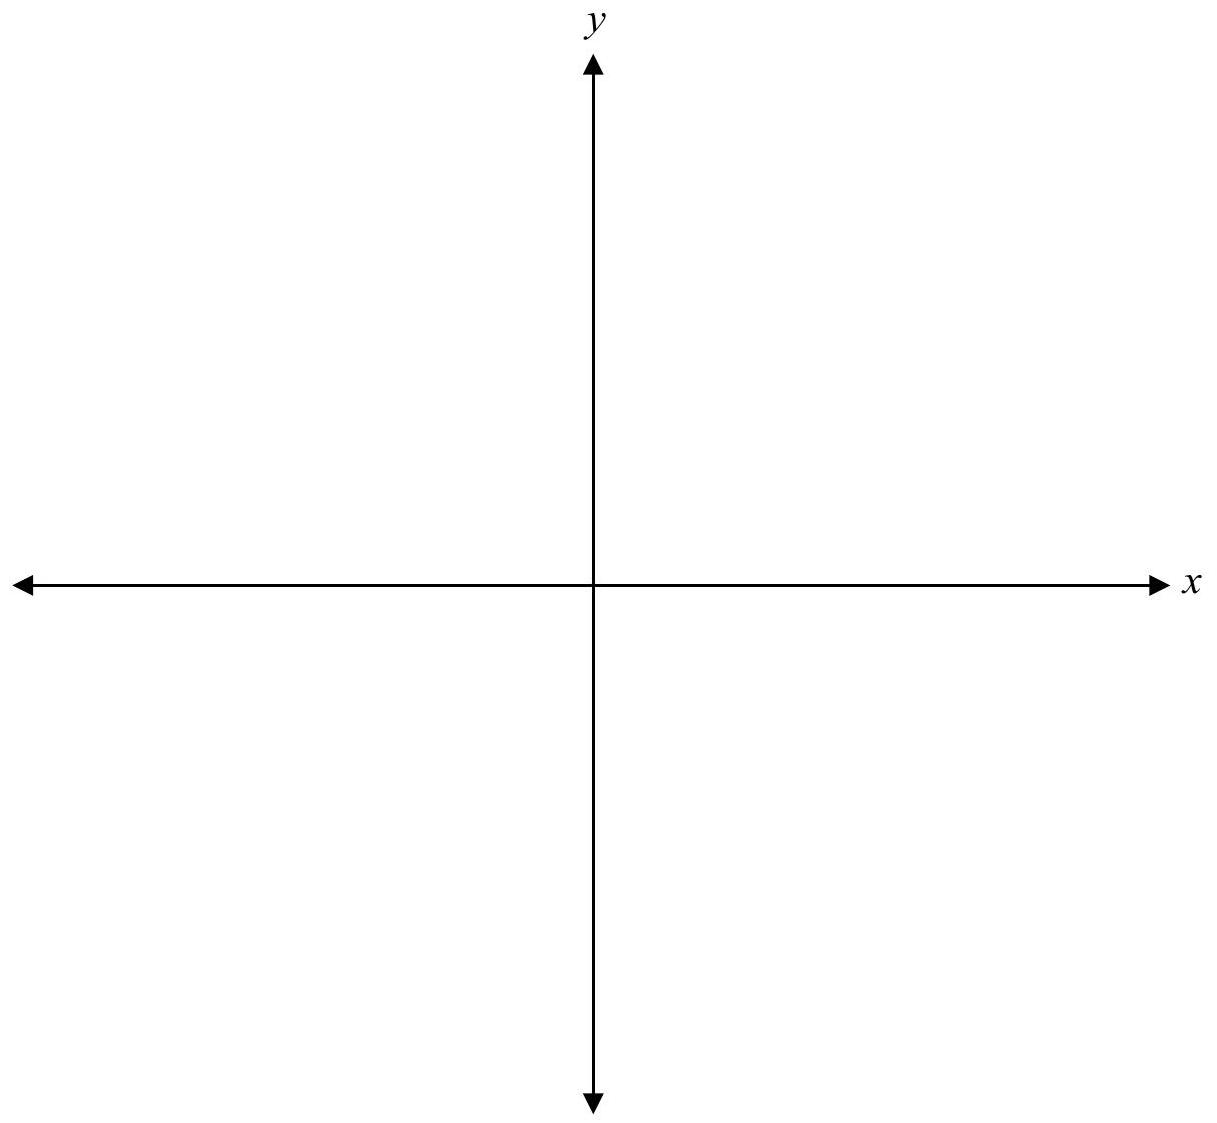
\includegraphics[max width=\textwidth, alt={}, center]{de5fb11a-28c7-4ac7-b7ff-0309cebac724-017_1123_1217_575_455}\\
$x$-intercepts: $\_\_\_\_$\\
$y$-intercept: $\_\_\_\_$

The graph of the function $y=\sin x$ has been transformed to create a new graph.\\
The range of this new graph is $[-4,4]$ and the zeros are $x=k \frac{\pi}{2}$, where $k$ is an integer. Write the equation that corresponds to this new graph.

Given the functions $f(x)=x^{2}-1$ and $g(x)=x+1$, state the domain of $\frac{g(x)}{f(x)}$.\\
a) Sketch the graph of $y=3^{x}$.\\
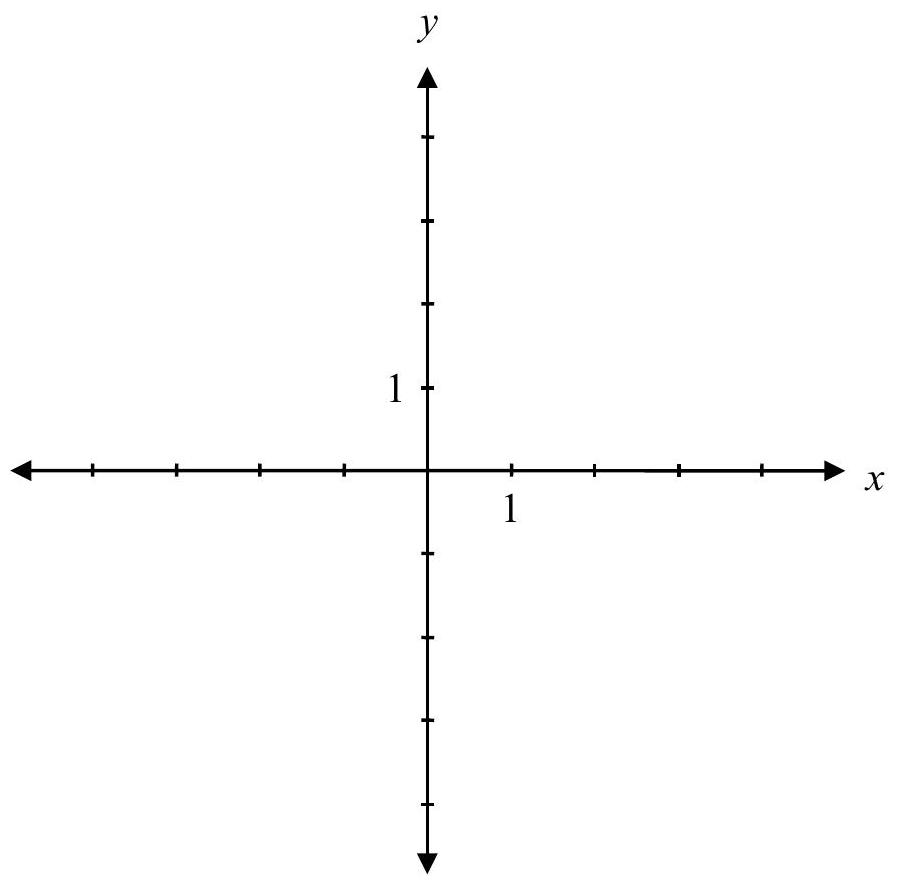
\includegraphics[max width=\textwidth, alt={}, center]{de5fb11a-28c7-4ac7-b7ff-0309cebac724-019_884_899_541_655}\\
b) Explain how the graph of $y=3^{x}$ can be used to sketch the graph of $y=\log _{3} x$.

A box in the shape of a rectangular prism has side lengths $x, x+2$ and $x+10$.\\
Write a function, $V(x)$, to express the volume of the box in terms of $x$.\\
Find all possible values of $x$, given that the volume of the box is $96 \mathrm{~cm}^{3}$.\\
State the dimensions of the box.

Given the graph of $f(x)$ below, sketch the graph of $y=-f(x)$.\\
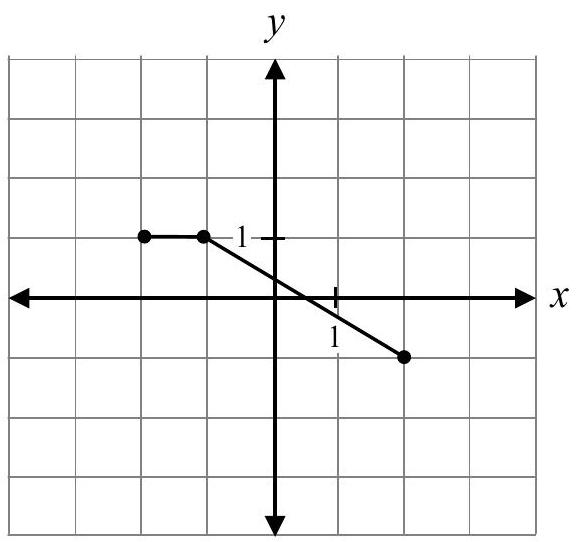
\includegraphics[max width=\textwidth, alt={}, center]{de5fb11a-28c7-4ac7-b7ff-0309cebac724-021_542_579_571_262}\\
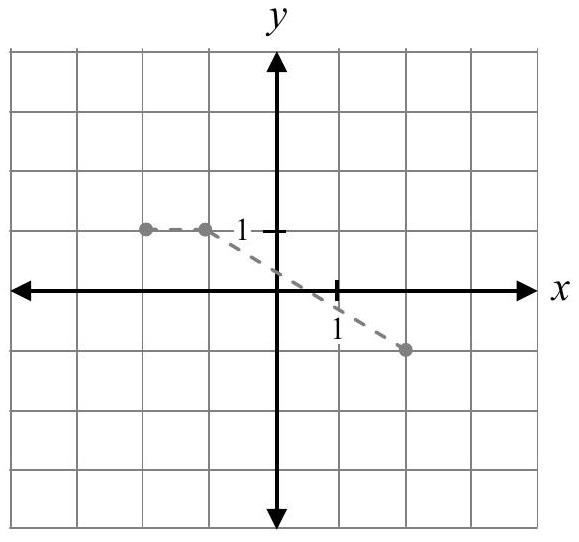
\includegraphics[max width=\textwidth, alt={}, center]{de5fb11a-28c7-4ac7-b7ff-0309cebac724-021_542_579_569_947}

The graph of $f(x)$ has already been drawn for your reference. No marks will be awarded for the graph of $f(x)$.

Determine the coordinates of a point $(x, y)$ on the unit circle if you are given $\theta=30^{\circ}$ where $\theta$ is in standard position.

Given the following sinusoidal equation:

$$
\mathrm{P}(t)=3000 \sin \left[\frac{\pi}{10}(t-2010)\right]+10000
$$

Determine the maximum value of $\mathrm{P}(t)$ and a value of $t$ at which this maximum occurs.

Maximum value of $\mathrm{P}(t)$ : $\_\_\_\_$

Value of $t$ : $\_\_\_\_$

Sketch the graph of $y=\sqrt{2 x-2}$.\\
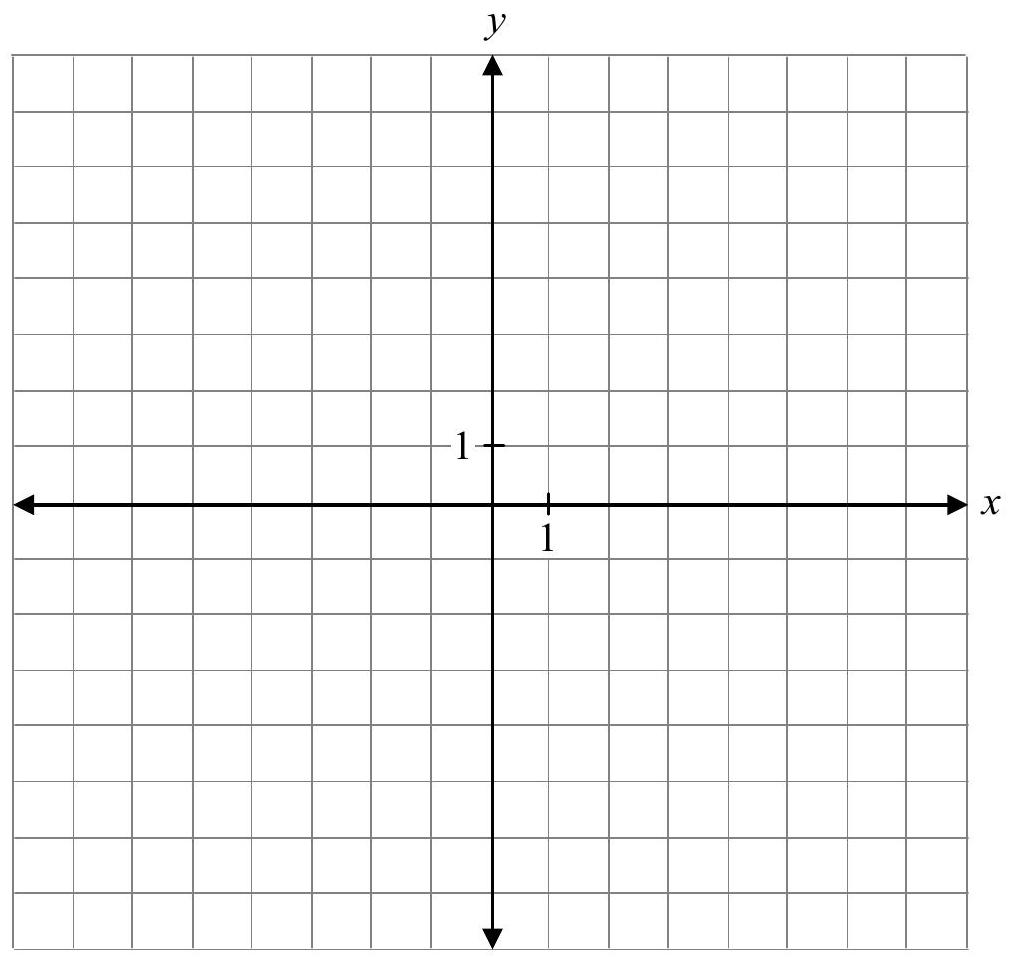
\includegraphics[max width=\textwidth, alt={}, center]{de5fb11a-28c7-4ac7-b7ff-0309cebac724-023_957_1013_524_554}

Given $f(x)=2 x-6$, write the equation of $f^{-1}(x)$.

Frank tried to expand a logarithmic expression using the laws of logarithms. He made one error.\\
Frank's solution: $\log _{a} \frac{(x+2)}{z w}=\log _{a} x+\log _{a} 2-\log _{a} z-\log _{a} w$\\
Write the correct solution.

Determine all non-permissible values of $\theta$ over the interval $[0,2 \pi]$.

$$
\frac{\sin \theta}{1+\cos \theta}+\csc \theta+\cot \theta
$$

Explain your reasoning.

\section*{Question 39}
Given the following graphs:\\
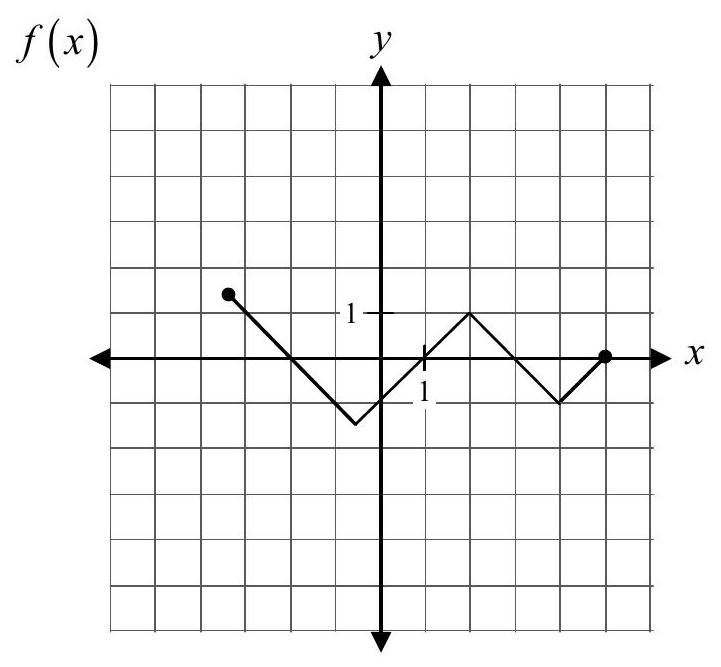
\includegraphics[max width=\textwidth, alt={}, center]{de5fb11a-28c7-4ac7-b7ff-0309cebac724-026_667_721_476_283}\\
a) 1 mark\\
b) 1 mark\\
c) 1 mark\\
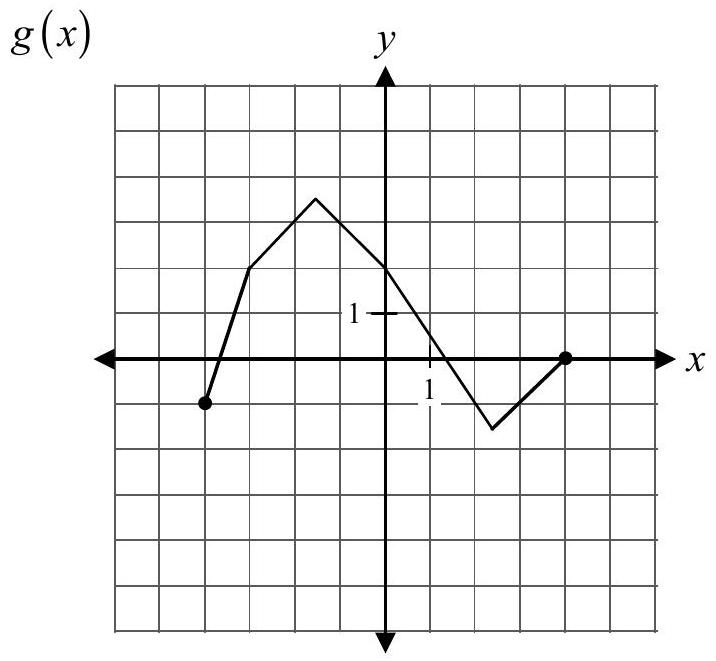
\includegraphics[max width=\textwidth, alt={}, center]{de5fb11a-28c7-4ac7-b7ff-0309cebac724-026_661_716_485_1119}\\
a) Determine the value of $[f \cdot g](0)$.\\
b) Determine the value of $g(f(4))$.\\
c) Determine a value for $k$ where $f(k)=1$.

Given that $h(x)=2 x^{2}+5 x-3$ and that $h(x)=f(x) \cdot g(x)$, determine $f(x)$ and $g(x)$.

The graph of $y=2 \cos \theta+1$ below can be used to solve the equation $\cos \theta=-\frac{1}{2}$ over the interval $[-2 \pi, 2 \pi]$. Indicate on the graph where to find the solutions to the equation $\cos \theta=-\frac{1}{2}$.\\
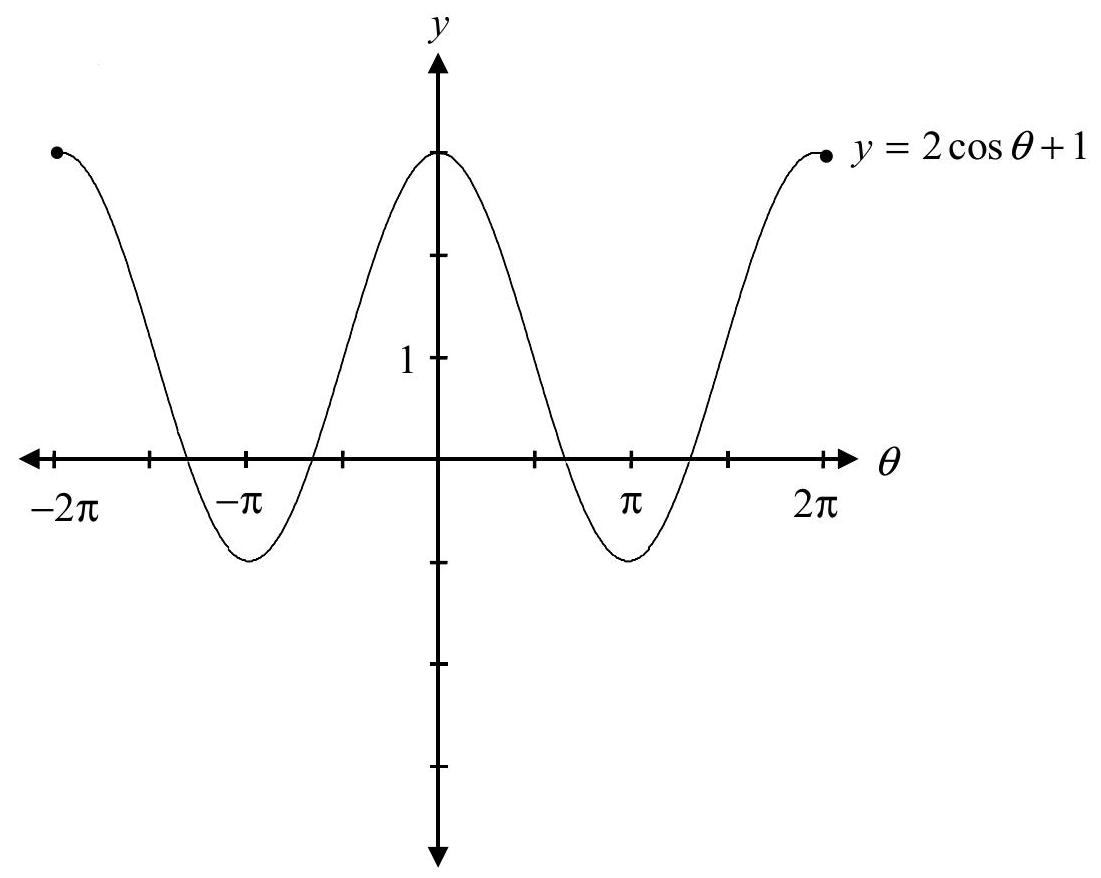
\includegraphics[max width=\textwidth, alt={}, center]{de5fb11a-28c7-4ac7-b7ff-0309cebac724-027_878_1101_1572_590}

The function $f(x)$ is transformed.\\
A new function, $y=\frac{1}{f(x)}$, is created that does not have any vertical asymptotes.\\
What can you conclude about the original function $f(x)$ ?

Question 43

Draw the angle $-\frac{7 \pi}{8}$ in standard position.\\
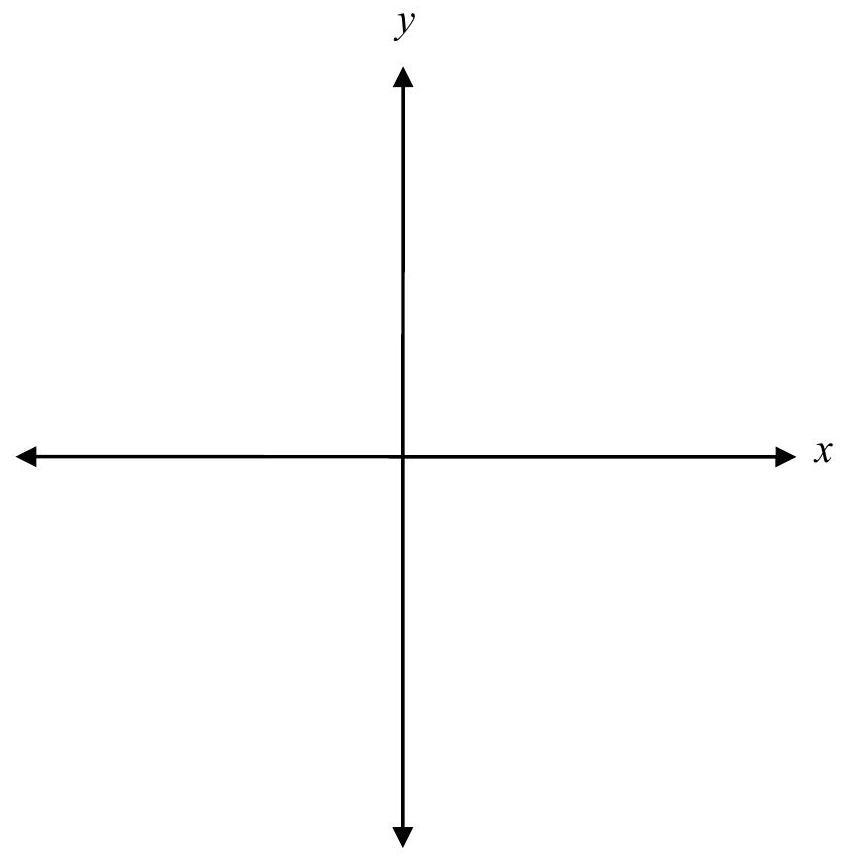
\includegraphics[max width=\textwidth, alt={}, center]{de5fb11a-28c7-4ac7-b7ff-0309cebac724-028_858_854_1602_612}

Determine the exact value of:

$$
4 \cos \left(\frac{11 \pi}{12}\right)
$$

Sketch the graph of $f(x)=\frac{x-4}{x^{2}-3 x-4}$.\\
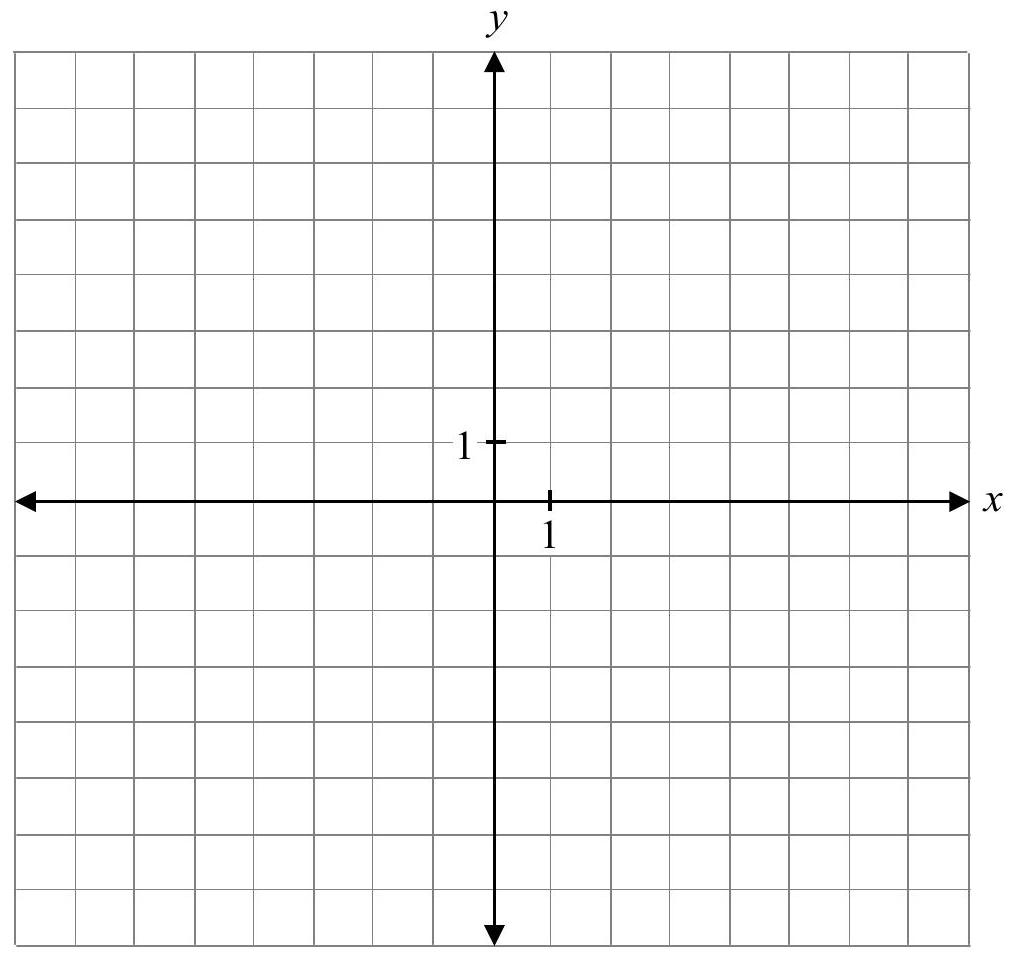
\includegraphics[max width=\textwidth, alt={}, center]{de5fb11a-28c7-4ac7-b7ff-0309cebac724-030_957_1015_567_620}

Estimate the value of $\log _{5} 35$.\\
Justify your answer.

If $p(x)=x^{5}-12 x+1$, determine the remainder when $p(x)$ is divided by $(x+2)$.

Describe the effects on the graph of $y=f(x)$ when asked for the graph of $y=f(x-3)+5$.

\section*{Question 49}
Find the exact value of the following expression:

$$
\sin \left(\frac{11 \pi}{3}\right) \cdot \sec \left(\frac{4 \pi}{3}\right) \cdot \tan \left(-\frac{5 \pi}{6}\right)
$$

A central angle of a circle subtends an arc length of $5 \pi \mathrm{~cm}$.\\
Given the circle has a radius of 9 cm , find the measure of the central angle in degrees.

Solve the equation $\csc ^{2} \theta+3 \csc \theta-4=0$ over the interval $[0,2 \pi]$.\\
Express your answers as exact values or correct to 3 decimal places.

Jess invests $\$ 12000$ at a rate of $4.75 \%$ compounded monthly. How long will it take for Jess to triple her investment?\\
Express your answer in years, correct to 3 decimal places.

The 4 th term in the binomial expansion of $\left(q x^{2}-\frac{3}{x}\right)^{10}$ is $414720 x^{11}$.\\
Determine the value of $q$ algebraically.

Bella has 2 pairs of shoes, 3 pairs of pants, and 10 shirts.\\
Carey has 4 pairs of shoes, 4 pairs of pants, and 4 shirts.\\
An outfit is made up of one pair of shoes, one pair of pants, and one shirt.\\
Who can make more outfits? Justify your answer.

Question 6\\
2 marks

In the binomial expansion of $(x-y)^{10}$, how many terms will be positive?\\
Justify your answer.

Solve the following equation algebraically where $180^{\circ} \leq \theta \leq 360^{\circ}$.

$$
2 \sin ^{2} \theta+5 \cos \theta+1=0
$$

Solve the following equation algebraically:

$$
\log _{3}(x-4)+\log _{3}(x-2)=1
$$

Given that $f(x)=\{(1,3),(2,5),(3,4),(4,2)\}$, find $f(f(3))$.

Given the graphs of $f(x)$ and $g(x)$ below,\\
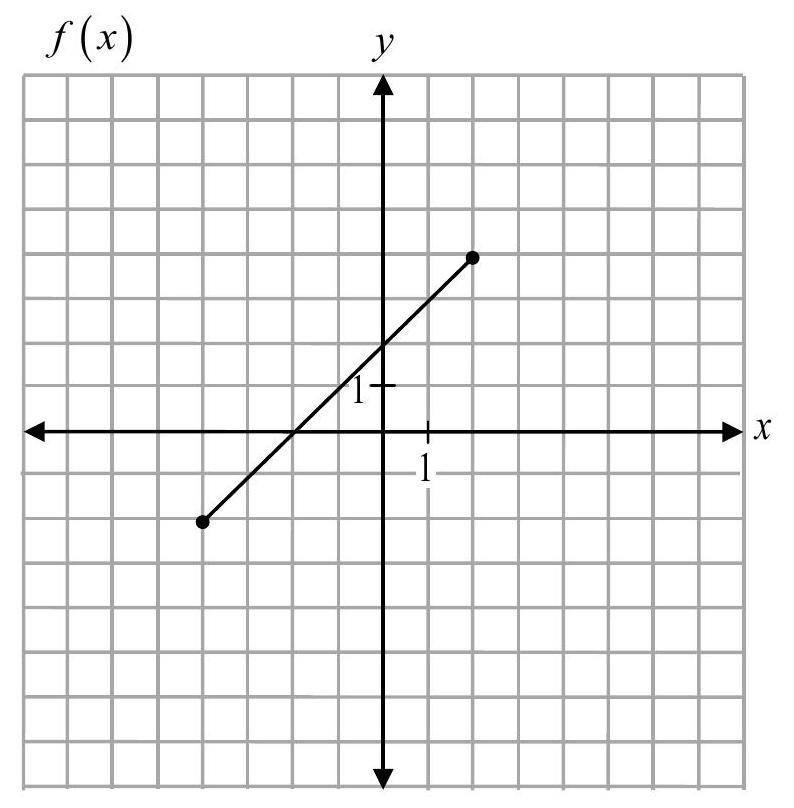
\includegraphics[max width=\textwidth, alt={}, center]{de5fb11a-28c7-4ac7-b7ff-0309cebac724-040_808_794_451_214}\\
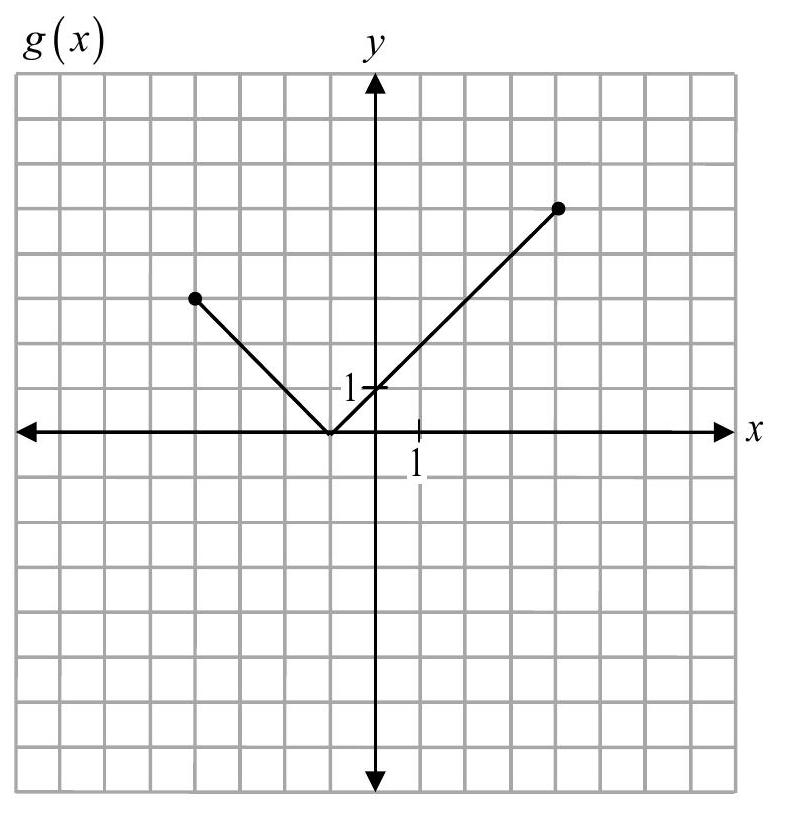
\includegraphics[max width=\textwidth, alt={}, center]{de5fb11a-28c7-4ac7-b7ff-0309cebac724-040_813_787_449_1117}\\
sketch the graph of $y=f(x)-g(x)$.\\
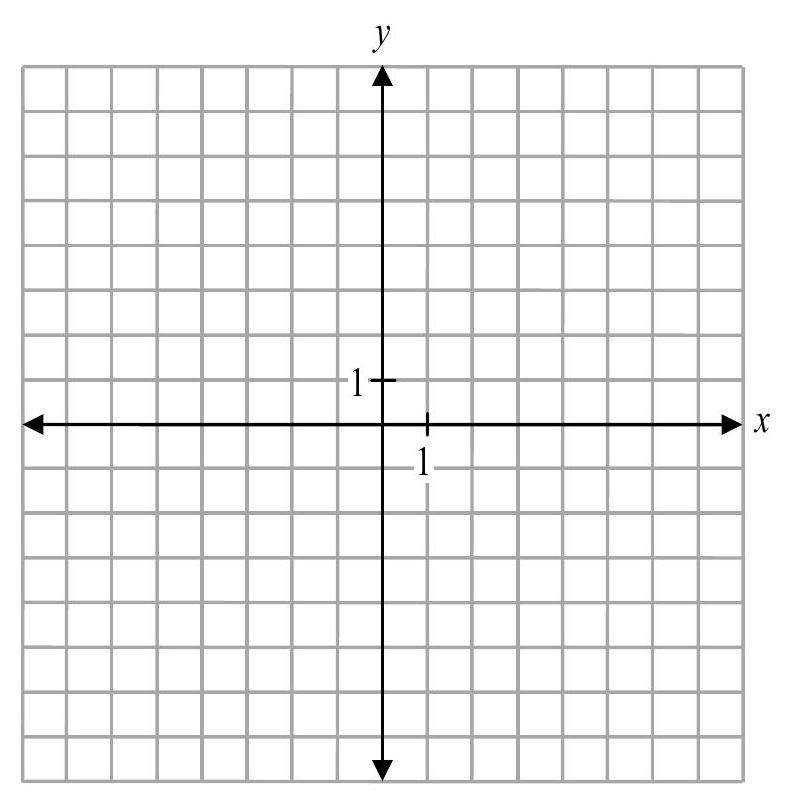
\includegraphics[max width=\textwidth, alt={}, center]{de5fb11a-28c7-4ac7-b7ff-0309cebac724-040_806_794_1521_212}

Given the graph of $y=f(x)$, describe the transformations to obtain the graph of the function $y=f(2 x-6)$.

Given $f(x)=\{(-3,4),(2,7),(8,6)\}$, state the domain of the resulting function after $f(x)$ is reflected through the line $y=x$.

Determine the value of $y$ in the following equation:

$$
\log _{x} 27-\log _{x} 3=2 \log _{x} y
$$

Angle $\theta$, measuring $\frac{5 \pi}{4}$, is drawn in standard position as shown below.\\
Determine the measures of all angles in the interval $[-4 \pi, 2 \pi]$ that are coterminal with $\theta$.\\
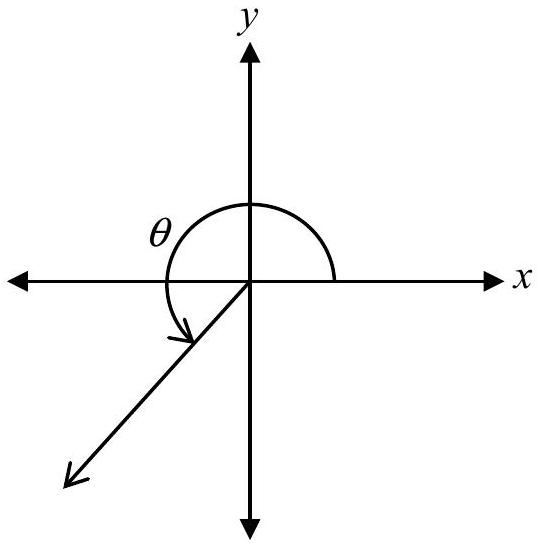
\includegraphics[max width=\textwidth, alt={}, center]{de5fb11a-28c7-4ac7-b7ff-0309cebac724-042_546_540_1914_326}

Prove the identity below for all permissible values of $x$ :

$$
\frac{\sin ^{2} x}{\sec x+1}=\cos x-\cos ^{2} x
$$

\begin{center}
\begin{tabular}{|l|l|}
\hline
Left-Hand Side & Right-Hand Side \\
\hline
\end{tabular}
\end{center}

Solve algebraically:

$$
{ }_{n} C_{2}=4 n+5
$$

How many different arrangements are possible when arranging all of the letters of the word SEPTEMBER?\\
a) 9 !\\
b) $6!3$ !\\
c) $\frac{9!}{3!}$\\
d) $\frac{6!}{3!}$

Question 18

Which one of the following angles terminates in Quadrant III?\\
a) 3 radians\\
b) $\frac{7 \pi}{5}$ radians\\
c) $-210^{\circ}$\\
d) $500^{\circ}$

There are 13 terms in the expansion of $(3 x-y)^{2 n}$. Determine the value of $n$.\\
a) 6\\
b) 6.5\\
c) 7\\
d) 26

Which of the following is true about the periods of the three functions below?

$$
f(\theta)=2 \sin 3\left(\theta-\frac{\pi}{2}\right) \quad g(\theta)=\sin 3 \theta+6 \quad k(\theta)=3 \sin \theta+6
$$

a) The graphs of $f(\theta)$ and $g(\theta)$ have the same period.\\
b) The graphs of $g(\theta)$ and $k(\theta)$ have the same period.\\
c) All of the graphs have the same period.\\
d) None of the graphs have the same period.

\section*{Question 21}
Which of the following represents the general solution to the equation $\tan \theta=-1$ ?\\
a) $\theta=\frac{\pi}{4}+2 k \pi, k \in \mathrm{I}$\\
b) $\theta=\frac{\pi}{4}+k \pi, k \in \mathrm{I}$\\
c) $\theta=\frac{3 \pi}{4}+2 k \pi, k \in \mathrm{I}$\\
d) $\theta=\frac{3 \pi}{4}+k \pi, k \in \mathrm{I}$

Question 22\\
1 mark

If $(3,-2)$ is a point on the graph of $y=f(x)$, what point must be on the graph of $y=2 f(x+1) ?$\\
a) $(4,-1)$\\
b) $(4,-4)$\\
c) $(2,1)$\\
d) $(2,-4)$

Which equation is represented by the graph sketched below?\\
a) $y=\left(\frac{1}{2}\right)^{-x}$\\
b) $y=\left(\frac{1}{2}\right)^{x}$\\
c) $y=2^{x}$\\
d) $y=-2^{x}$\\
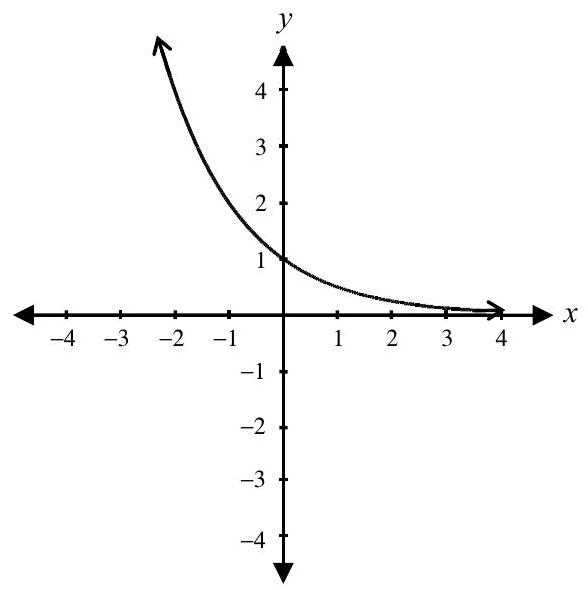
\includegraphics[max width=\textwidth, alt={}, center]{de5fb11a-28c7-4ac7-b7ff-0309cebac724-047_590_588_487_687}

Question 24\\
1 mark\\
What is the degree of the polynomial represented below?\\
a) 2\\
b) 3\\
c) 4\\
d) 5\\
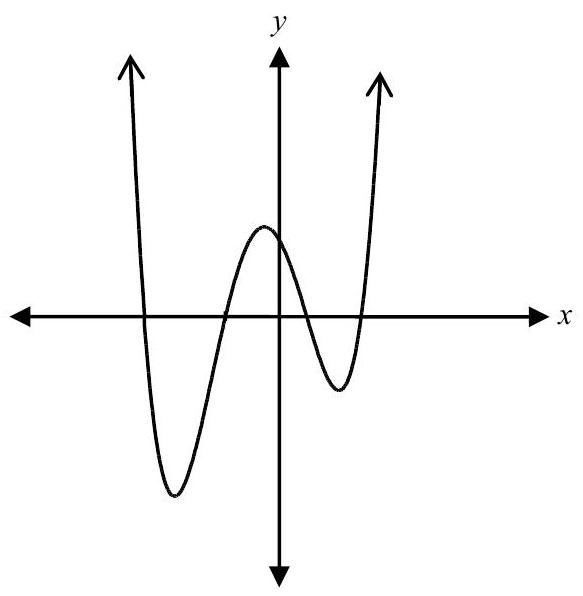
\includegraphics[max width=\textwidth, alt={}, center]{de5fb11a-28c7-4ac7-b7ff-0309cebac724-047_596_583_1658_661}

Given the graph of $y=2 \cos \pi x+1$ below, determine another equation that will produce the same graph.\\
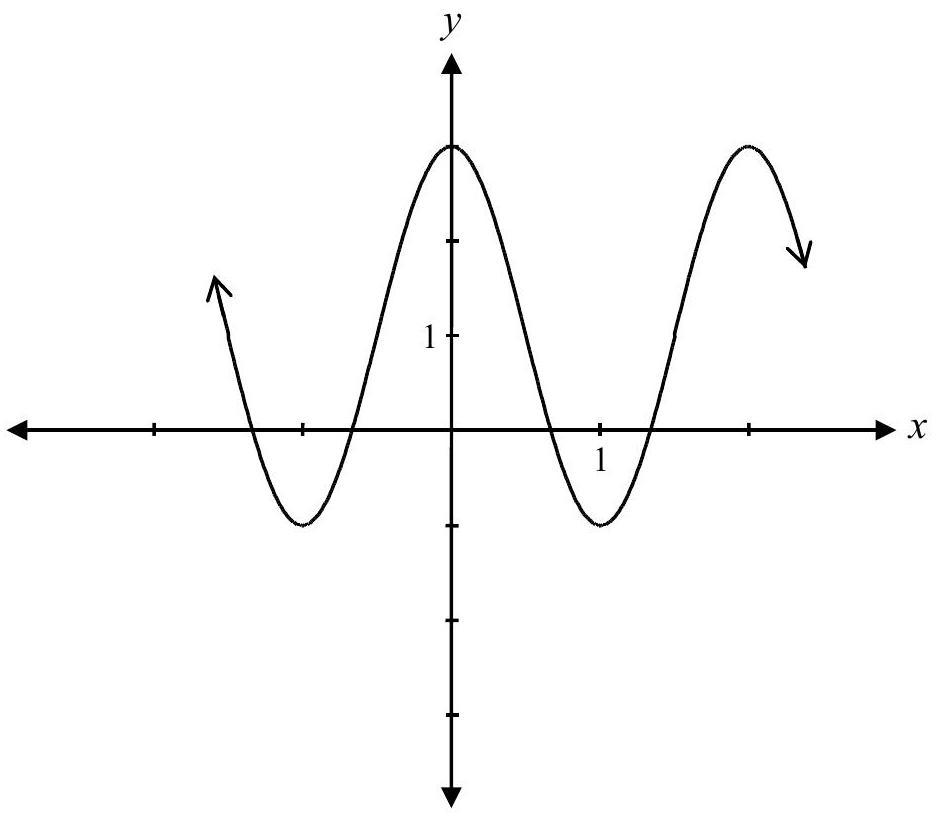
\includegraphics[max width=\textwidth, alt={}, center]{de5fb11a-28c7-4ac7-b7ff-0309cebac724-048_818_937_491_292}

$$
y=
$$

Given $f(x)=3$ and $g(x)=x+2$, determine the domain and range of $h(x)=\frac{f(x)}{g(x)}$.

Domain: $\_\_\_\_$\\
Range: $\_\_\_\_$

Explain how to find the exact value of $\sec \left(\frac{19 \pi}{6}\right)$.

Given $f(x)=4-x$, verify that $f^{-1}(x)=f(x)$.

Sketch the graph of:

$$
f(x)=(2-x)(x+3)(x+1)^{2}
$$

Label the $x$-intercepts and $y$-intercept.\\
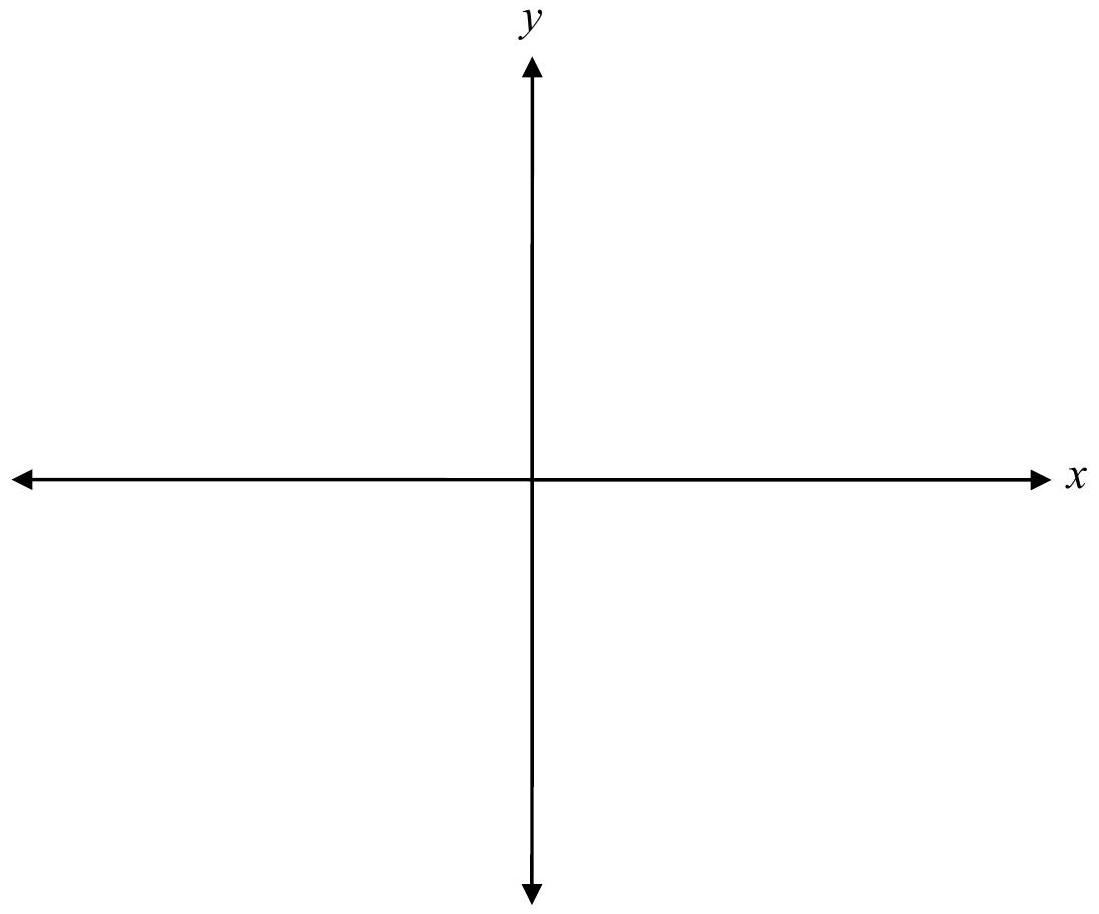
\includegraphics[max width=\textwidth, alt={}, center]{de5fb11a-28c7-4ac7-b7ff-0309cebac724-050_914_1099_706_438}

Which expression has a larger value?

$$
\log _{2} 36 \text { or } \log _{3} 80
$$

Justify your answer.

The graph below represents the equation $y=a x^{3}+6 x^{2}+5 x-10$.\\
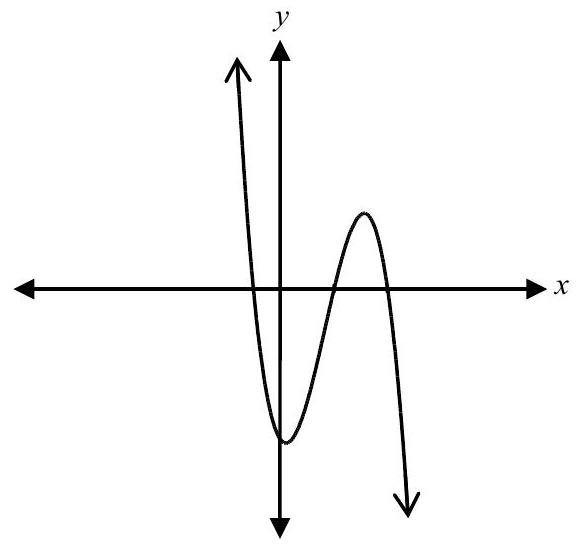
\includegraphics[max width=\textwidth, alt={}, center]{de5fb11a-28c7-4ac7-b7ff-0309cebac724-051_549_583_1450_348}

What must be true about the value of $a$ ? Explain your reasoning.

The terminal arm of an angle $\theta$, in standard position, intersects the unit circle in Quadrant IV at a point $\mathrm{P}\left(\frac{\sqrt{5}}{4}, y\right)$. Determine the value of $\sin \theta$.

Given the sinusoidal function $f(x)$ below, sketch the graph of $g(x)=|f(x)|-1$.\\
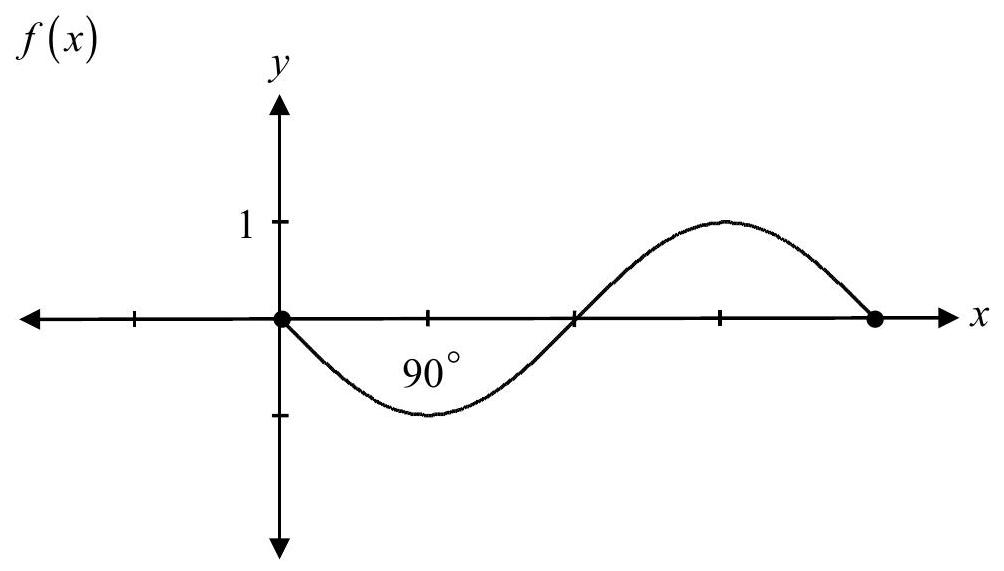
\includegraphics[max width=\textwidth, alt={}, center]{de5fb11a-28c7-4ac7-b7ff-0309cebac724-053_571_1004_519_522}\\
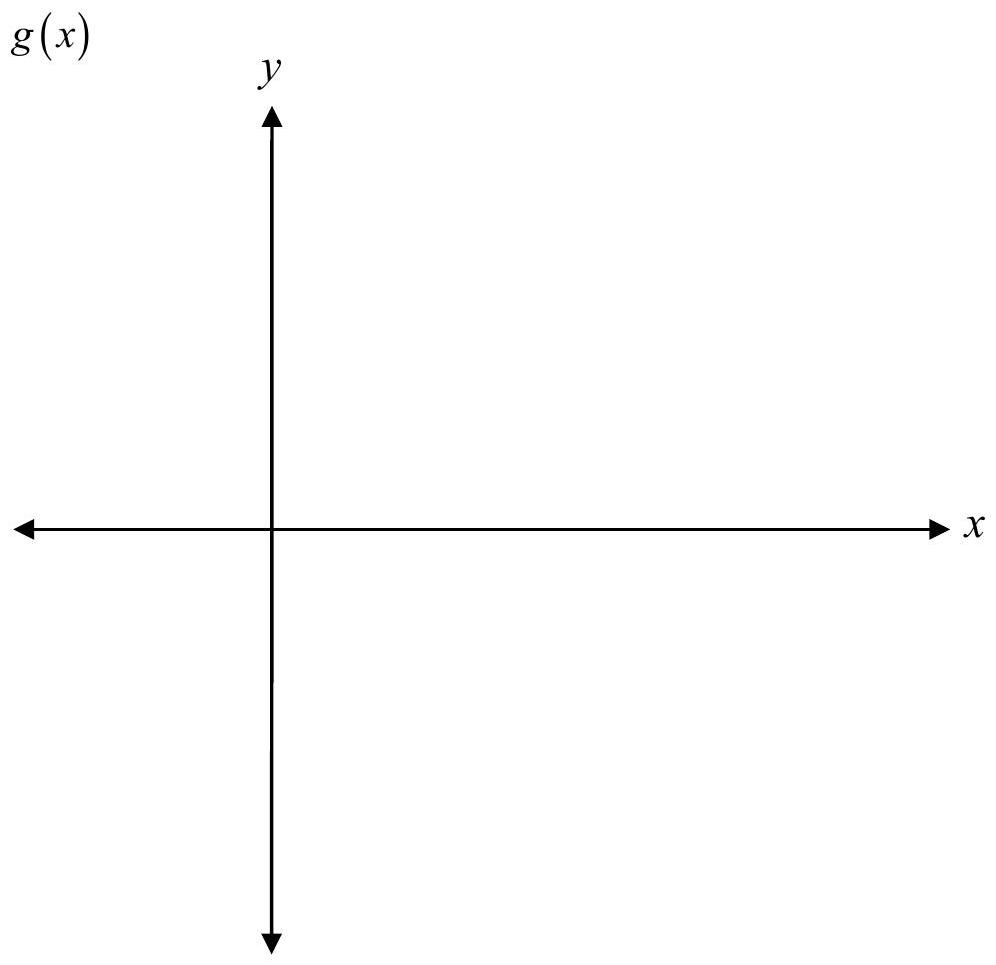
\includegraphics[max width=\textwidth, alt={}, center]{de5fb11a-28c7-4ac7-b7ff-0309cebac724-053_965_996_1263_528}

The graph of a rational function, $f(x)$, has a point of discontinuity when $x=2$ and an asymptote when $x=4$. Write a possible equation for $f(x)$.

Question 35

Given that $(x-1)$ is one of the factors, express $x^{3}-57 x+56$ as a product of factors.

Give an example using values for $A$ and $B$, in degrees or radians, to verify that $\cos (A+B)=\cos A+\cos B$ is not an identity.

\begin{center}
\begin{tabular}{|l|l|}
\hline
Left-Hand Side & Right-Hand Side \\
\hline
 &  \\
\hline
\end{tabular}
\end{center}

Sketch the graph of $y=\sqrt{x+1}-2$ and verify that the value of the $x$-intercept is the same as the solution to the equation $\sqrt{x+1}-2=0$.\\
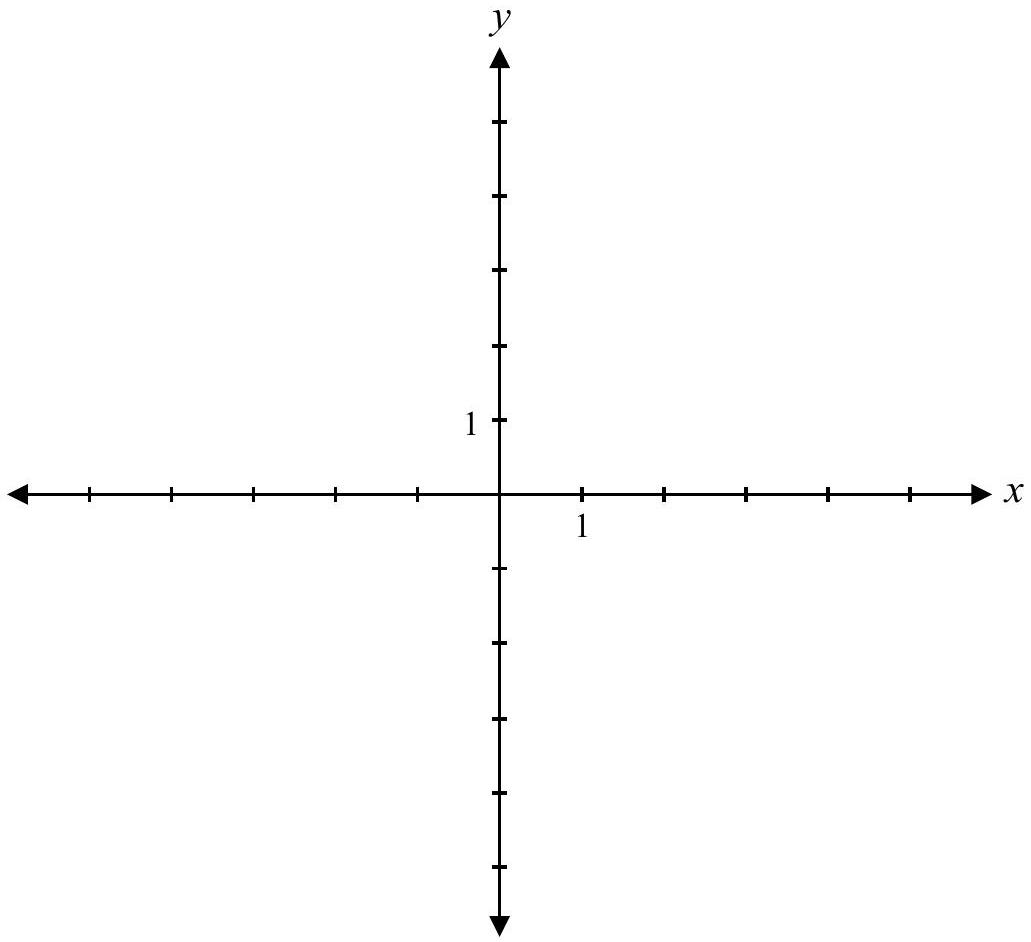
\includegraphics[max width=\textwidth, alt={}, center]{de5fb11a-28c7-4ac7-b7ff-0309cebac724-056_942_1031_627_592}

Mohamed is asked to sketch the graph of $y=\tan x$.\\
His graph is shown below.\\
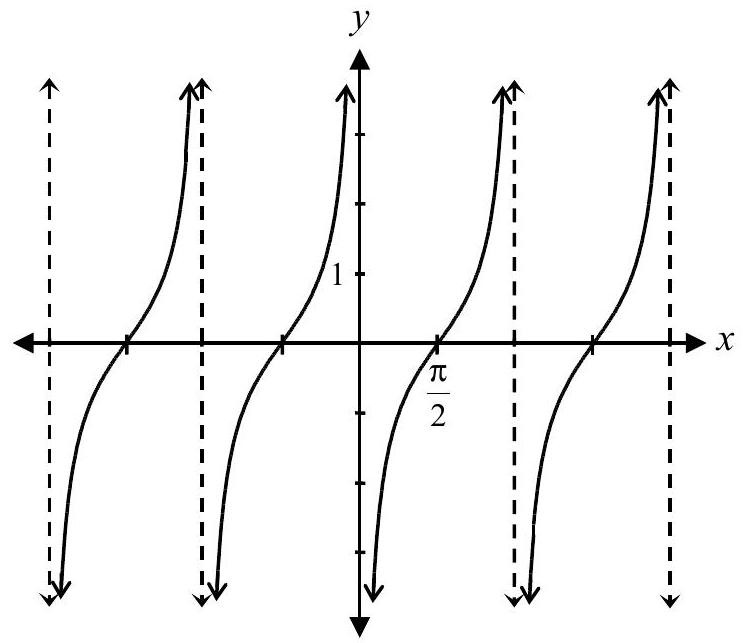
\includegraphics[max width=\textwidth, alt={}, center]{de5fb11a-28c7-4ac7-b7ff-0309cebac724-057_643_745_507_388}

Explain why his graph is incorrect.

On the interval $0 \leq \theta<2 \pi$, identify the non-permissible values of $\theta$ for the trigonometric identity:

$$
\tan \theta=\frac{1}{\cot \theta}
$$

a) Sketch the graph of $y=\ln (x)$.\\
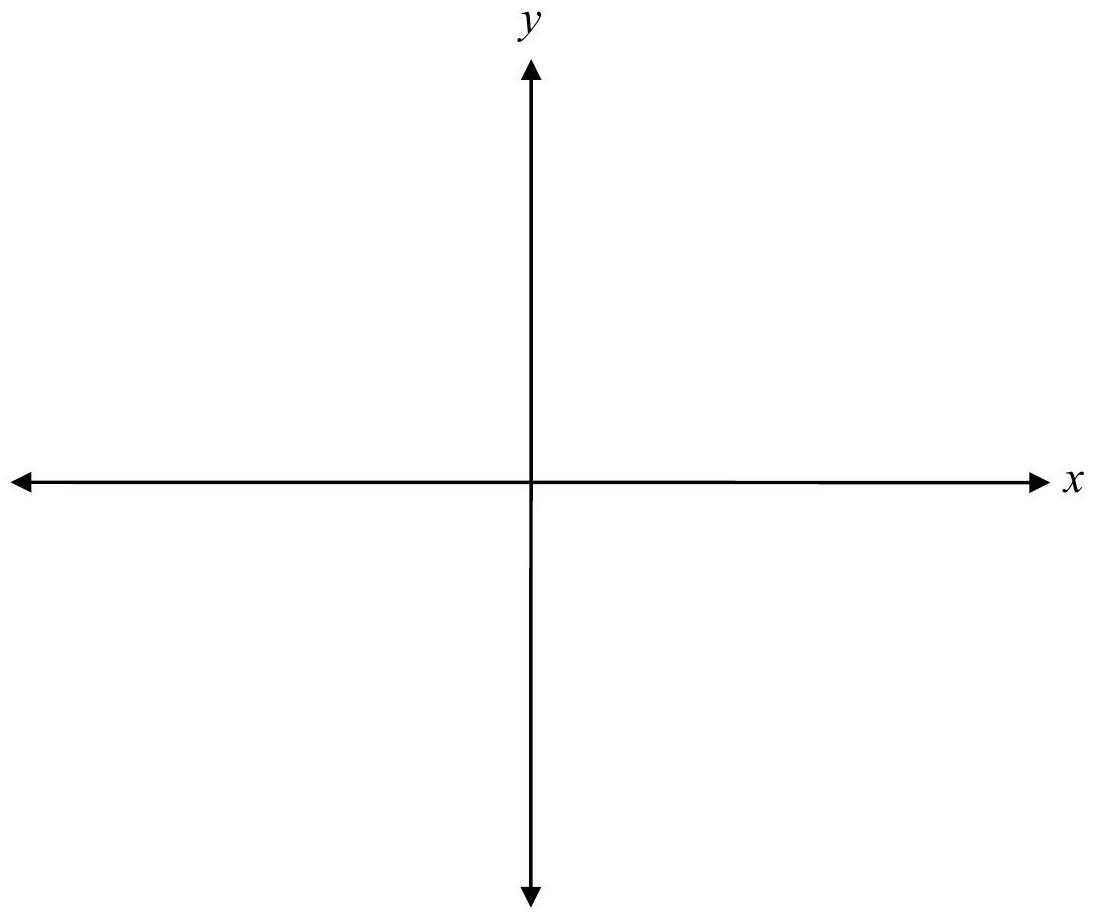
\includegraphics[max width=\textwidth, alt={}, center]{de5fb11a-28c7-4ac7-b7ff-0309cebac724-059_916_1095_453_532}\\
b) Sketch the graph of $y=-\ln (x-2)$.\\
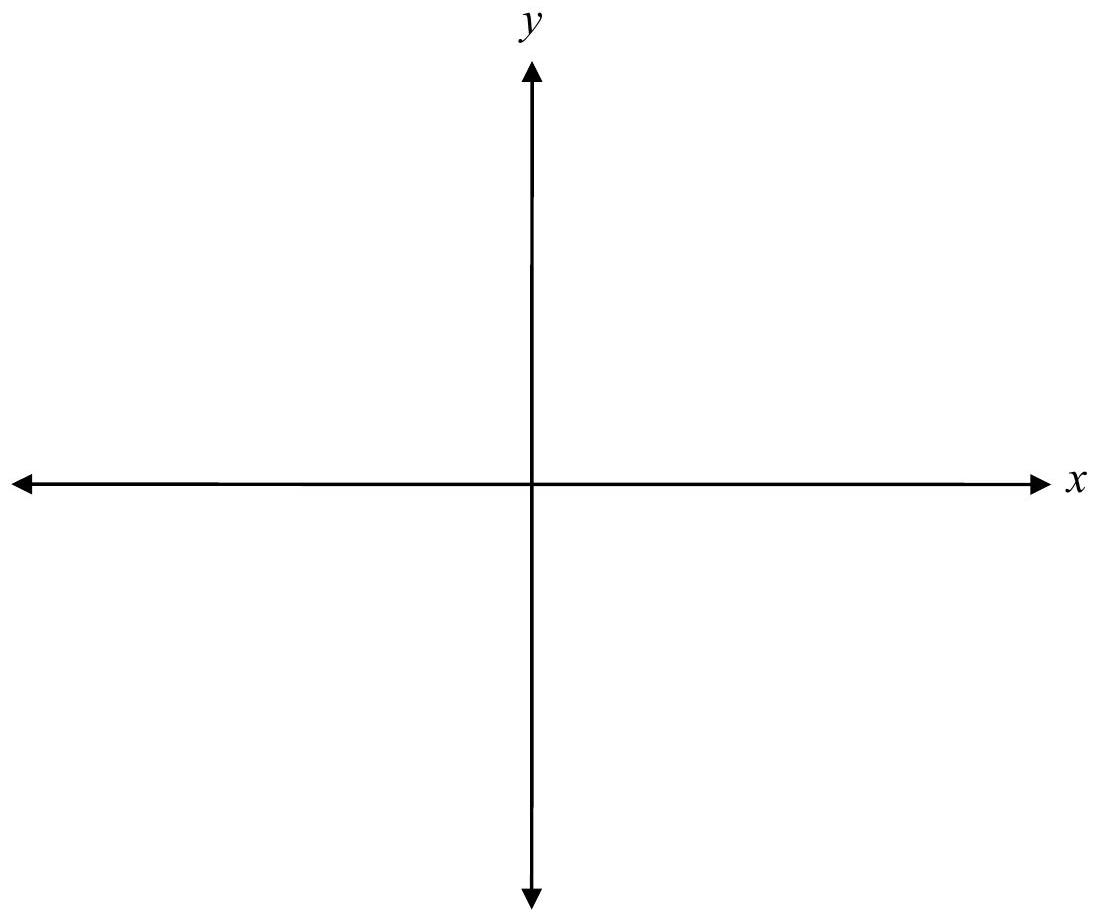
\includegraphics[max width=\textwidth, alt={}, center]{de5fb11a-28c7-4ac7-b7ff-0309cebac724-059_918_1097_1570_528}

Given $f(x)=\sqrt{x-2}$ and $g(x)=3 x$, write the equation for $h(x)=f(g(x))$.\\
What are the restrictions on the domain of $h(x)$ ?\\
Explain your reasoning.

Sketch the graph of $y=10 \cos \left[\frac{\pi}{2}(x-2)\right]$ over the interval $[0,6]$.\\
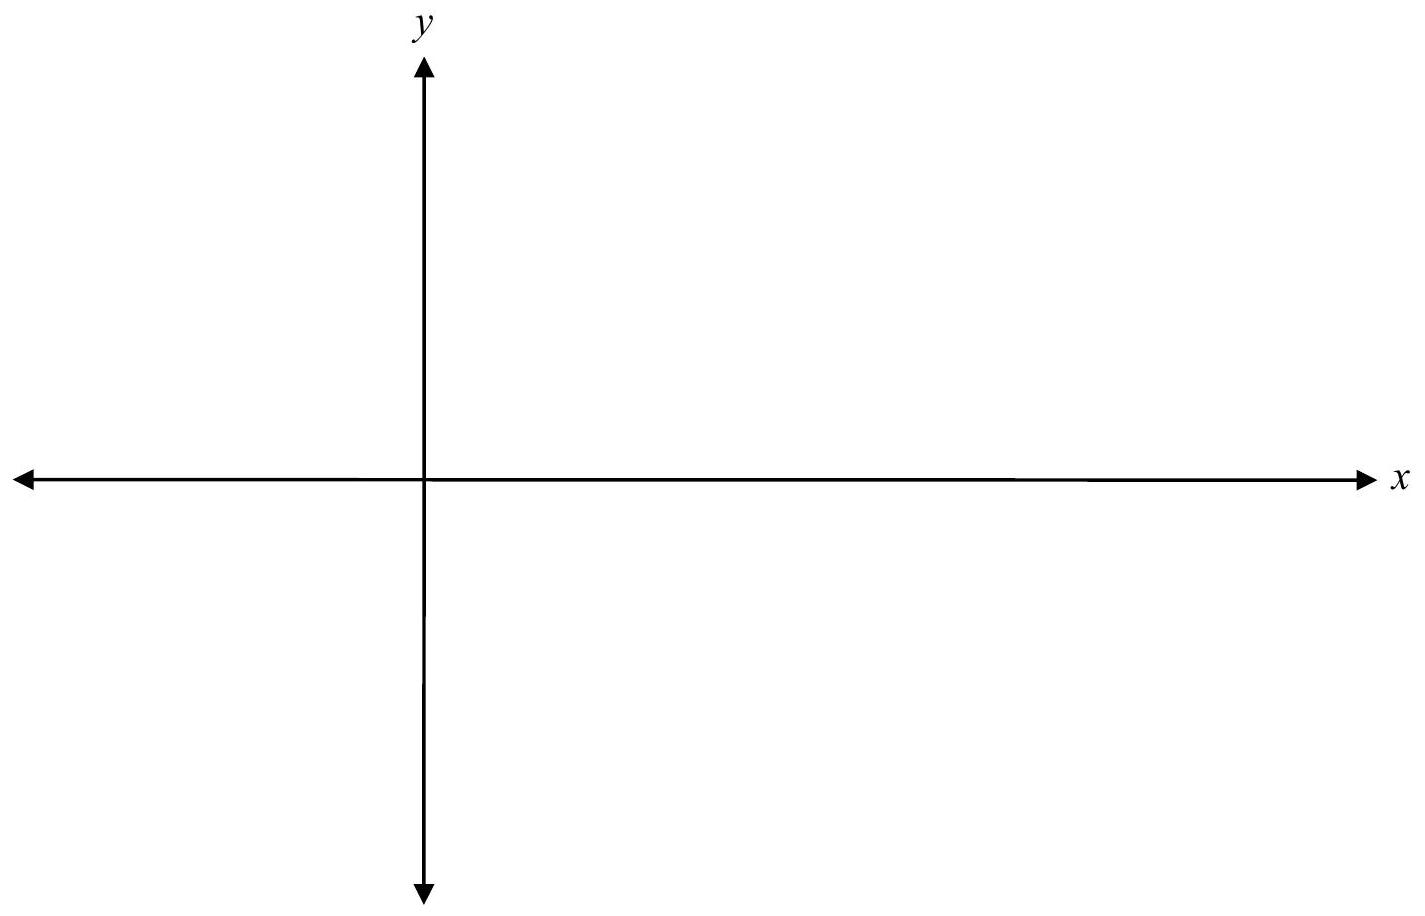
\includegraphics[max width=\textwidth, alt={}, center]{de5fb11a-28c7-4ac7-b7ff-0309cebac724-061_916_1425_623_436}

Sketch the graph of the function $f(x)=\frac{x^{2}}{x^{2}-x}$.\\
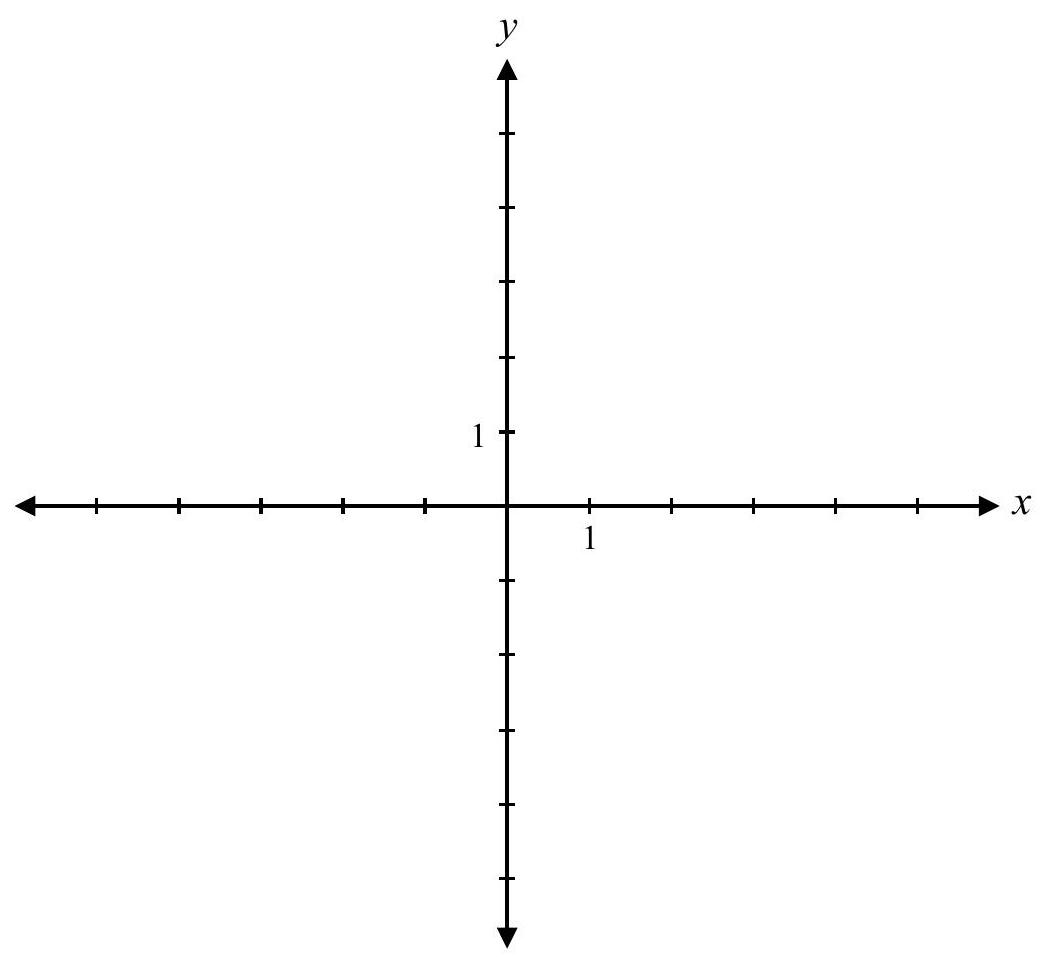
\includegraphics[max width=\textwidth, alt={}, center]{de5fb11a-28c7-4ac7-b7ff-0309cebac724-062_963_1050_623_588}

Is $(x-3)$ a factor of $x^{4}-x^{3}-3 x^{2}+x-1$ ?\\
Justify your answer.

Given $f(x)=x-1$ and $g(x)=x^{2}$, write the equation of $y=f(g(x))$ and sketch the graph.\\
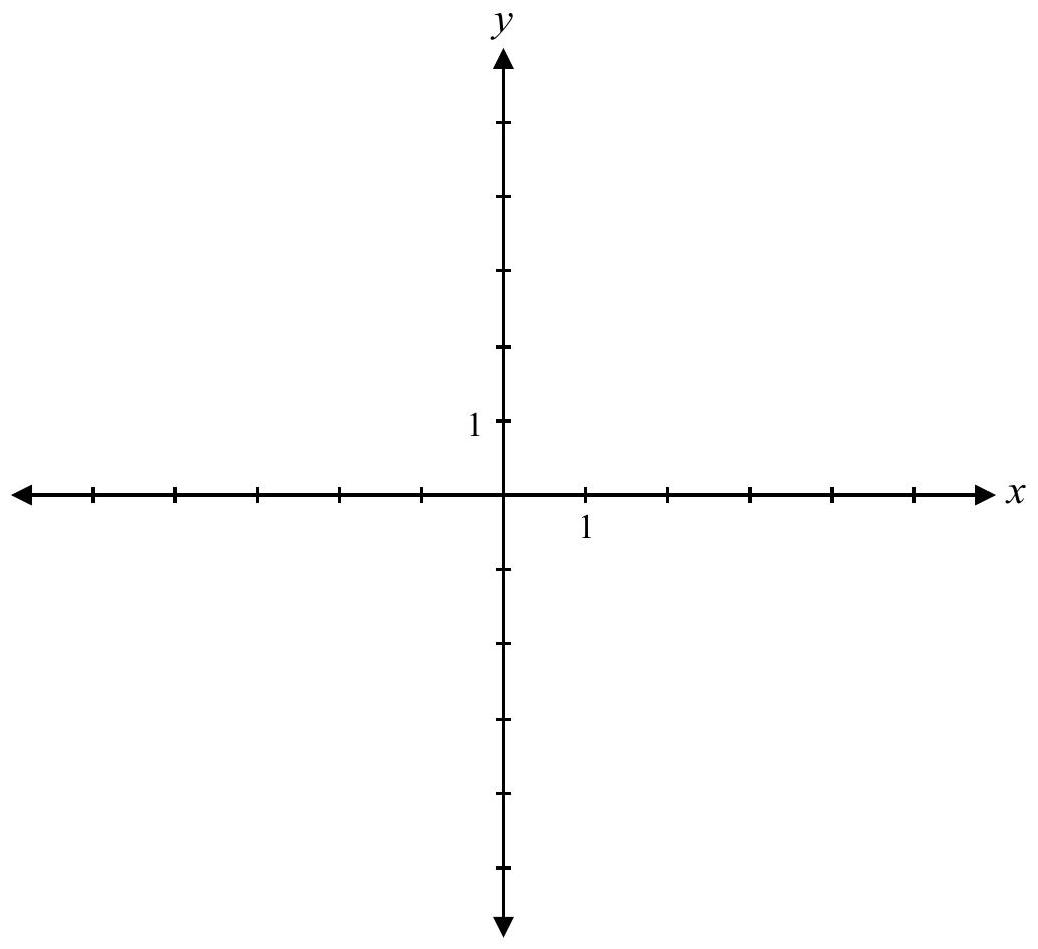
\includegraphics[max width=\textwidth, alt={}, center]{de5fb11a-28c7-4ac7-b7ff-0309cebac724-064_949_1038_519_550}

Find the coterminal angle to $\frac{27 \pi}{5}$ over the interval $\left[-360^{\circ}, 0^{\circ}\right)$.

Solve the following equation over the interval $0 \leq \theta<2 \pi$.

$$
(\tan \theta-3)(\tan \theta+1)=0
$$

An earthquake in Vancouver had a magnitude of 6.3 on the Richter scale. An earthquake in Japan had a magnitude of 8.9 on the Richter scale.\\
How many times more intense was the Japan earthquake than the Vancouver earthquake?\\
You may use the formula below:

$$
M=\log \left(\frac{A}{A_{0}}\right)
$$

where $M$ is the magnitude of the earthquake on the Richter scale\\
$A$ is the intensity of the earthquake\\
$A_{0}$ is the intensity of a standard earthquake\\
Express your answer as a whole number.

Find and simplify the last term in the expansion of $(2 y-3 x)^{7}$.

Given $\log _{a} 9=1.129$ and $\log _{a} 4=0.712$, find the value of $\log _{a} 12$.

How many different ways can 4 girls and 4 boys be arranged in a row if the girls and the boys must alternate?

Solve the following equation over the interval $[0,2 \pi]$.

$$
2 \cos 2 \theta-1=0
$$

Alex incorrectly explains to Rashid that the graph of $y=2 f(x)+5$ means you first move the graph of $y=f(x)$ up 5 units and then multiply the $y$ values by 2 .

Explain to Rashid the correct way to transform the graph.

Sketch the angle of 5 radians in standard position.\\
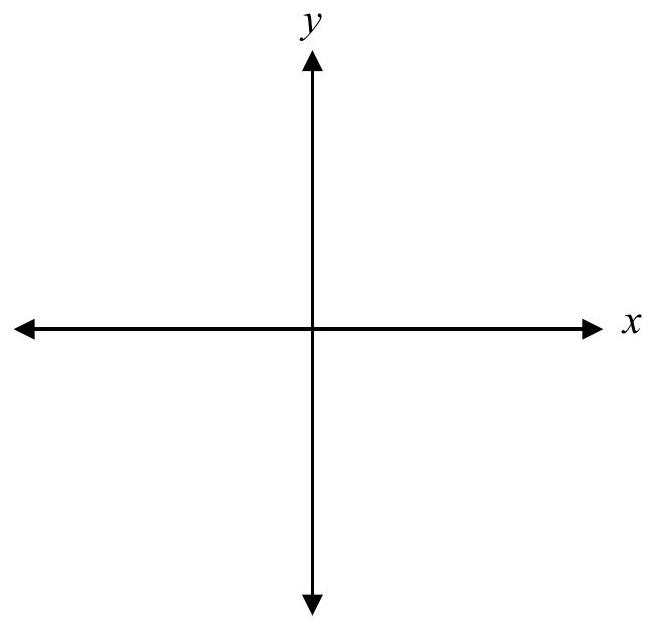
\includegraphics[max width=\textwidth, alt={}, center]{de5fb11a-28c7-4ac7-b7ff-0309cebac724-072_624_654_1675_711}

Given the graphs of $f(x)$ and $(f-g)(x)$, sketch the graph of $g(x)$.\\
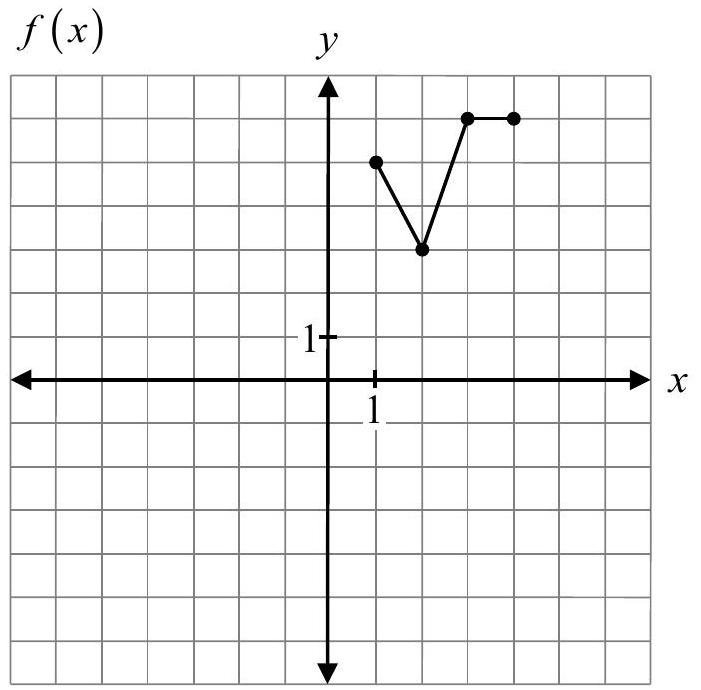
\includegraphics[max width=\textwidth, alt={}, center]{de5fb11a-28c7-4ac7-b7ff-0309cebac724-073_690_701_554_281}\\
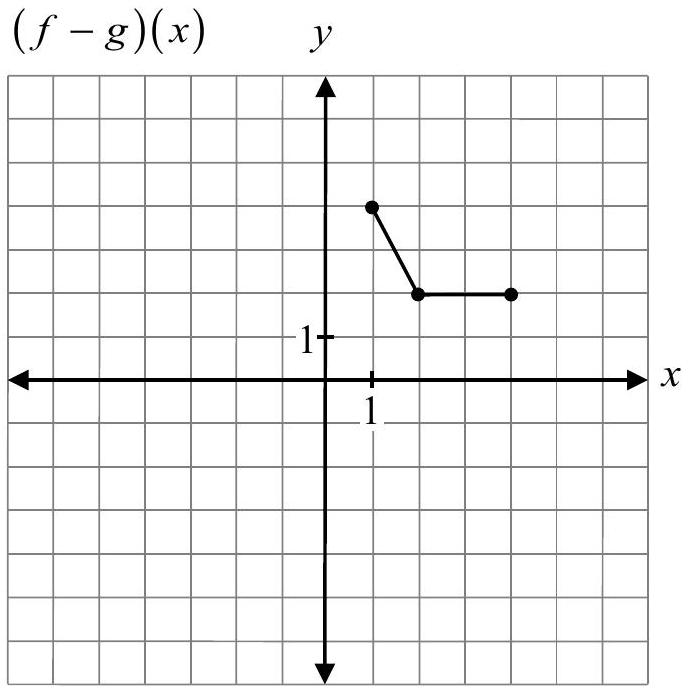
\includegraphics[max width=\textwidth, alt={}, center]{de5fb11a-28c7-4ac7-b7ff-0309cebac724-073_693_690_554_1158}\\
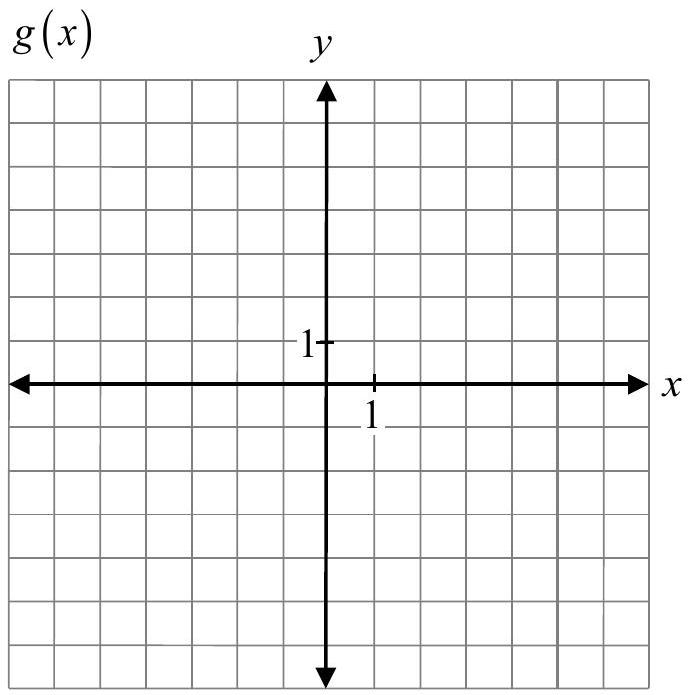
\includegraphics[max width=\textwidth, alt={}, center]{de5fb11a-28c7-4ac7-b7ff-0309cebac724-073_695_688_1417_728}

A particular math class has a large number of students. From this class, you are to create a committee of 4 students that has at least 1 girl.\\
Without actually solving the problem, explain the strategy you would use to find the total number of ways to select this committee.\\
a) Prove the identity below for all permissible values of $\theta$.

$$
\frac{1+2 \cos ^{2} \theta}{\cos ^{2} \theta}=\tan ^{2} \theta+3
$$

\begin{center}
\begin{tabular}{|l|l|}
\hline
Left-Hand Side & Right-Hand Side \\
\hline
 &  \\
\hline
\end{tabular}
\end{center}

b) Determine all the non-permissible values for $\theta$.

Given the graph of $f(x)$ below,\\
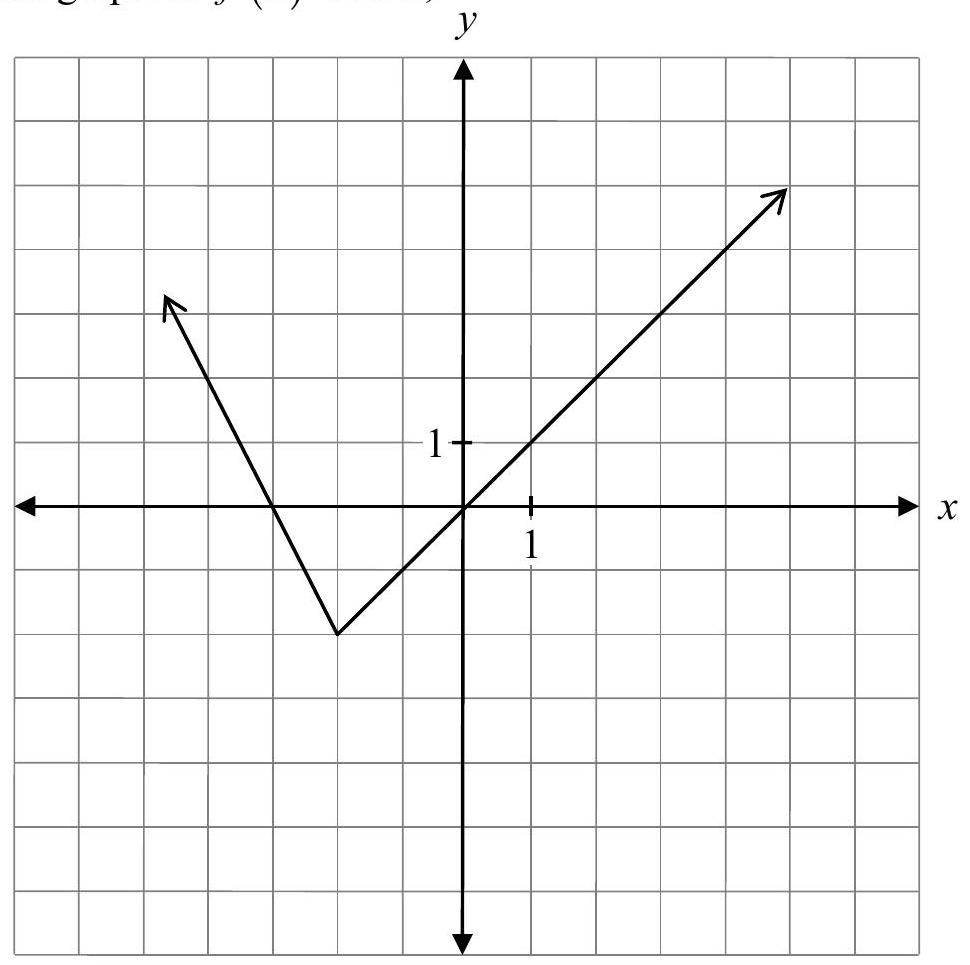
\includegraphics[max width=\textwidth, alt={}, center]{de5fb11a-28c7-4ac7-b7ff-0309cebac724-076_965_970_421_369}\\
sketch the graph of $g(x)=f(x-2)+3$.\\
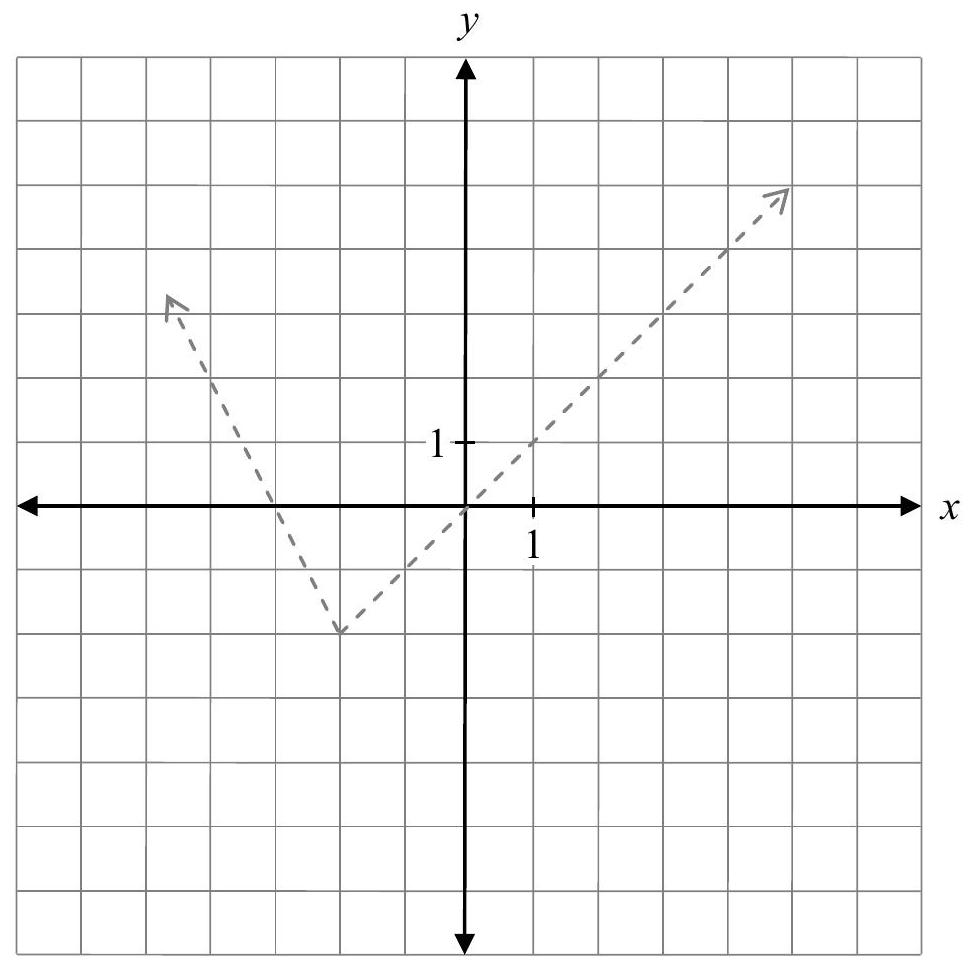
\includegraphics[max width=\textwidth, alt={}, center]{de5fb11a-28c7-4ac7-b7ff-0309cebac724-076_965_970_1523_373}

The graph of $f(x)$ has already been drawn for your reference.\\
No marks will be awarded for the graph of $f(x)$.

Given that $\sin \alpha=\frac{5}{13}$, where $\alpha$ is in Quadrant II, and $\cos \beta=\frac{2}{5}$, where $\beta$ is in Quadrant IV, find the exact value of:\\
a) $\cos (\alpha+\beta)$\\
b) $\sin 2 \alpha$

If $f(x)=x^{3}$ and $g(x)=2 x-3$, what is the value of $\left(\frac{f}{g}\right)(-1) ?$

If the point $(4,-3)$ lies on the graph of $f(x)$, which point must lie on the graph of $2 f(2 x)$ ?\\
a) $(8,-6)$\\
b) $(2,-6)$\\
c) $\left(8,-\frac{3}{2}\right)$\\
d) $\left(2,-\frac{3}{2}\right)$

Question 17

The graph of $y=\log _{2}(2 x+6)$ intersects the graph of $y=4$ at:\\
a) $x=-1$\\
b) $x=1$\\
c) $x=5$\\
d) $x=14$

Given the point $\mathrm{A}(-3,5)$ on the terminal arm of an angle $\theta$, identify the value of $\cot \theta$.\\
a) $-\frac{3}{5}$\\
b) $-\frac{5}{3}$\\
c) $-\frac{4}{5}$\\
d) $-\frac{5}{4}$

\section*{Question 19}
The graph of $y=\left(\frac{1}{2}\right)^{x}$ compared to the graph of $x=\left(\frac{1}{2}\right)^{y}$ is a:\\
a) reflection in the $x$-axis\\
b) reflection in the $y$-axis\\
c) reflection in the line $y=x$\\
d) reciprocal function

\section*{Question 20}
1 mark\\
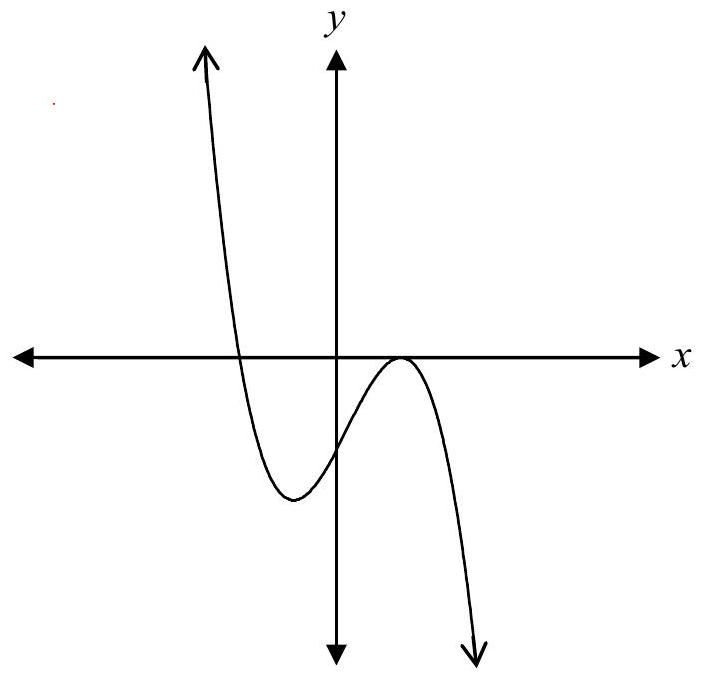
\includegraphics[max width=\textwidth, alt={}, center]{de5fb11a-28c7-4ac7-b7ff-0309cebac724-080_682_708_1151_313}

Given the above graph of a polynomial function, which one of the following statements can be true?\\
a) The function has a degree of 4 with a positive leading coefficient.\\
b) The function has a degree of 4 with a negative leading coefficient.\\
c) The function has a degree of 3 with a positive leading coefficient.\\
d) The function has a degree of 3 with a negative leading coefficient.

Given that $(x+3)$ is a factor of polynomial $P(x)$, which of the following is true?\\
a) $P(-3)=0$\\
b) $P(0)=-3$\\
c) $P(0)=3$\\
d) $P(3)=0$

\section*{Question 22}
Which of the following is a reasonable estimate for the value of $\log 350$ ?\\
a) 2\\
b) 2.5\\
c) 2.8\\
d) 3

\section*{Question 23}
The graph of the function $f(x)$ shown below is best described by the equation:\\
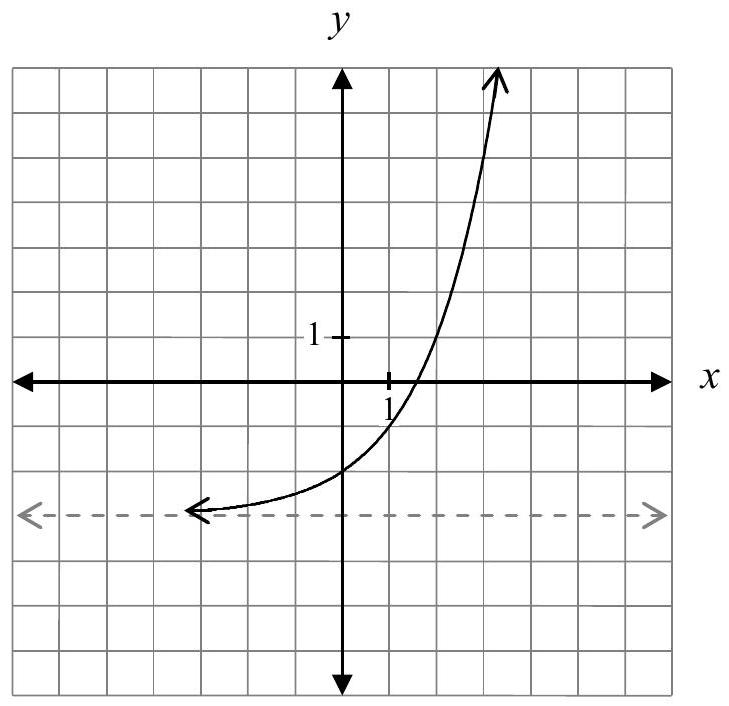
\includegraphics[max width=\textwidth, alt={}, center]{de5fb11a-28c7-4ac7-b7ff-0309cebac724-081_706_729_1600_335}\\
a) $f(x)=2^{x+3}$\\
b) $f(x)=2^{x}+3$\\
c) $f(x)=2^{x-3}$\\
d) $f(x)=2^{x}-3$

Given the graph of $y=f(x)$, what is the domain of $\sqrt{f(x)}$ ?\\
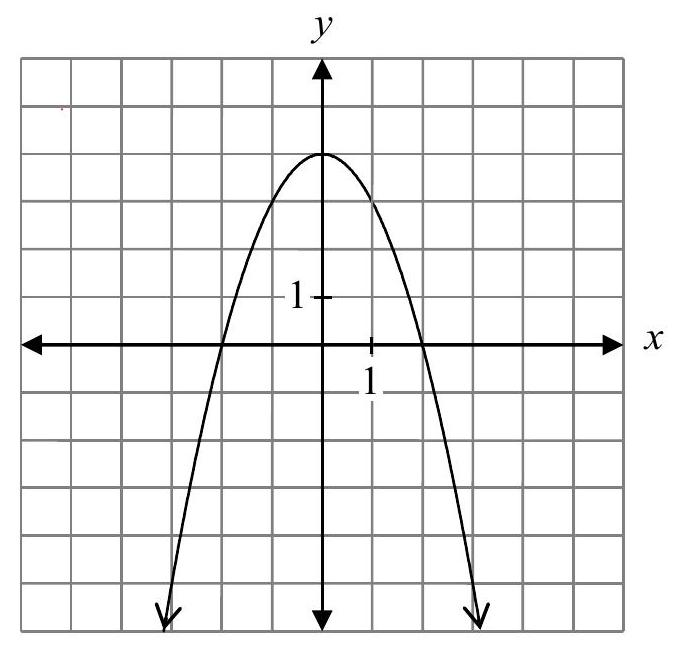
\includegraphics[max width=\textwidth, alt={}, center]{de5fb11a-28c7-4ac7-b7ff-0309cebac724-082_645_676_483_317}\\
a) $x \in \mathbb{R}$\\
b) $-2 \leq x \leq 2$\\
c) $x \leq-2$ or $x \geq 2$\\
d) $0 \leq x \leq 4$

Solve:

$$
e^{\ln (5-x)}=7
$$

a) -2\\
b) $-\ln 2$\\
c) $\ln 7-\ln 5$\\
d) $\frac{7}{5}$

One of the factors of $P(x)=x^{3}-k x^{2}-7 x+10$ is $(x-2)$.\\
Find the value of $k$.\\
a) Sketch the graph of the function $y=\sqrt{-x}+1$.\\
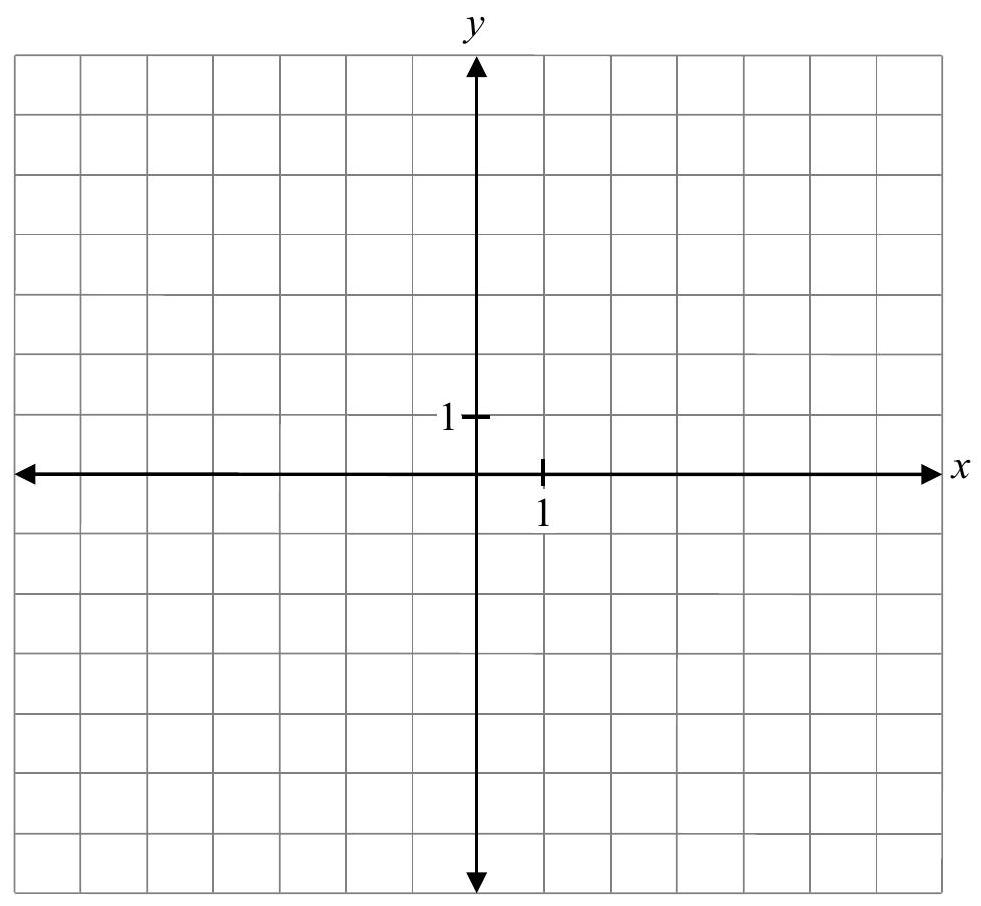
\includegraphics[max width=\textwidth, alt={}, center]{de5fb11a-28c7-4ac7-b7ff-0309cebac724-084_906_981_489_519}\\
b) Determine the value of $x$ when $y=3$.

Solve the following equation:

$$
{ }_{n} P_{2}={ }_{n} C_{3}
$$

Given $f(x)=x^{2}-1$ and $g(x)=\sqrt{x+1}$, sketch the graph of $y=f(g(x))$ and state its domain.\\
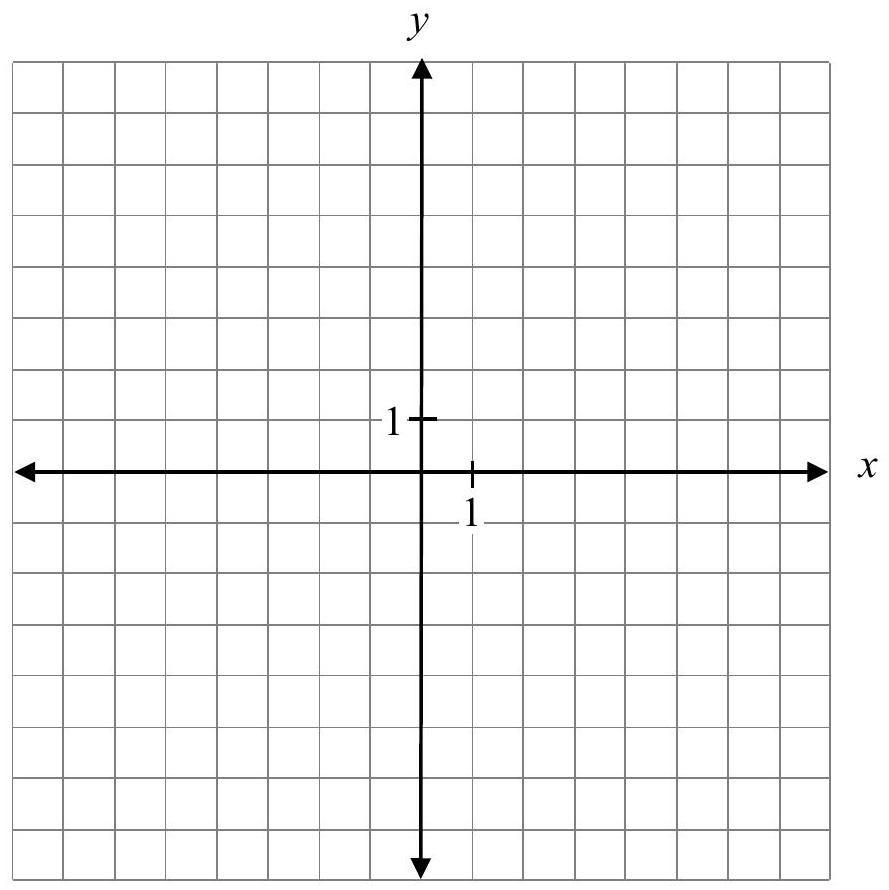
\includegraphics[max width=\textwidth, alt={}, center]{de5fb11a-28c7-4ac7-b7ff-0309cebac724-086_890_889_498_603}

Domain: $\_\_\_\_$

Write the equation of the horizontal asymptote for the function $f(x)=\frac{x-3}{x-2}$.

The $x$-intercept of $f(x)$ is 4 and the $x$-intercept of $g(x)$ is 4 .\\
Benjamin concludes that the $x$-intercept of $f(x)+g(x)$ is 8 .\\
Do you agree with Benjamin? Justify your answer.

Solve the following equation:

$$
2 \log _{4} x-\log _{4}(x+3)=1
$$

\section*{Question 33}
The following graph represents tidal levels in the Bay of Fundy over a 25 -hour period.\\
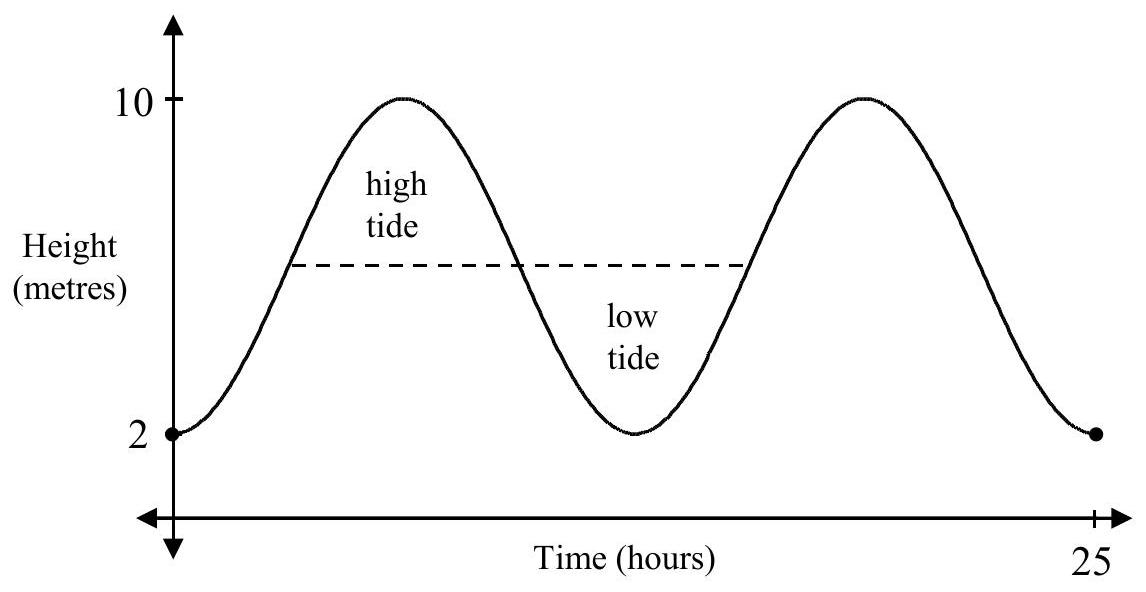
\includegraphics[max width=\textwidth, alt={}, center]{de5fb11a-28c7-4ac7-b7ff-0309cebac724-089_592_1146_442_296}\\
a) What is the average height of the water?\\
b) What is the period of the graph above?

Explain what the period represents in this situation.

Given the graph of $y=f(x)$ below,\\
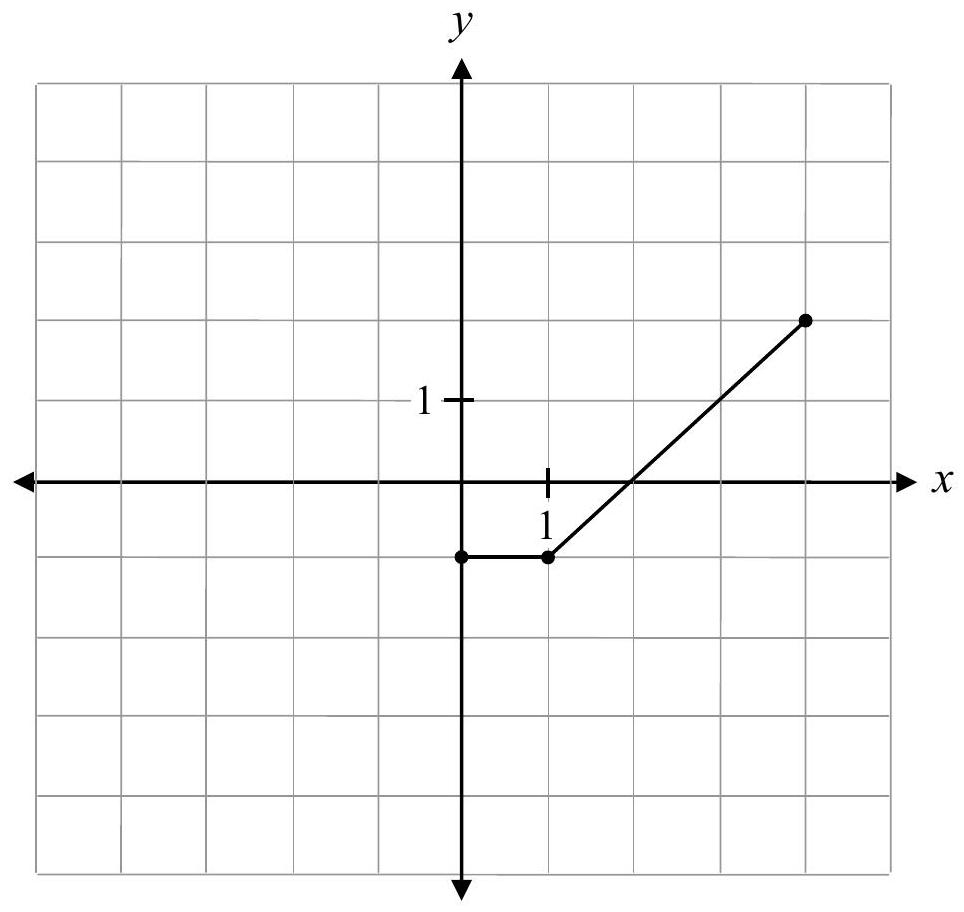
\includegraphics[max width=\textwidth, alt={}, center]{de5fb11a-28c7-4ac7-b7ff-0309cebac724-090_912_964_470_298}\\
sketch the graph of $y=\sqrt{f(x)}$.\\
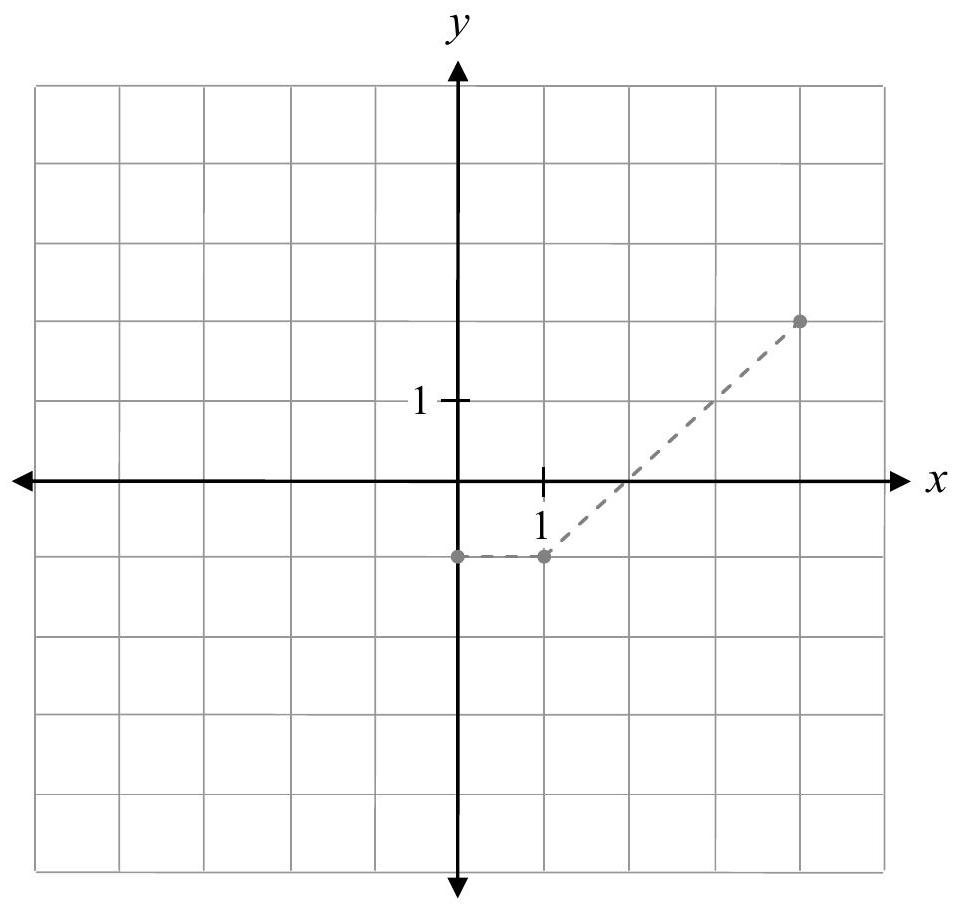
\includegraphics[max width=\textwidth, alt={}, center]{de5fb11a-28c7-4ac7-b7ff-0309cebac724-090_912_964_1536_298}

The graph of $f(x)$ has already been drawn for your reference.\\
No marks will be awarded for the graph of $f(x)$.

When $P(x)$ is divided by $x-3$, it has a quotient of $2 x^{2}+x-6$ and a remainder of 4 .\\
Determine $P(x)$.

\section*{Question 36}
Identify the domain and range of the following function:

$$
f(x)=\frac{3}{x^{2}+1}
$$

Evaluate:

$$
\csc \left(\frac{11 \pi}{6}\right)+\sin ^{2}\left(-\frac{3 \pi}{4}\right)+\cos \left(\frac{23 \pi}{3}\right)
$$

Evaluate the coefficient of the term containing $x^{3}$ in the expansion of $(1+x)^{7}$.\\
Justify your answer.

Which of the following equations could be solved without the use of logarithms?\\
Without actually solving the problem, explain your choice.

$$
4^{x}=10^{3 x+1} \quad \text { or } \quad\left(\frac{1}{3}\right)^{2 x+1}=27^{4 x-1}
$$

Sketch the graph of $y=x^{3}+x^{2}-5 x+3$ given that one of the $x$-intercepts is 1 .\\
Identify the $x$-intercepts and $y$-intercept.\\
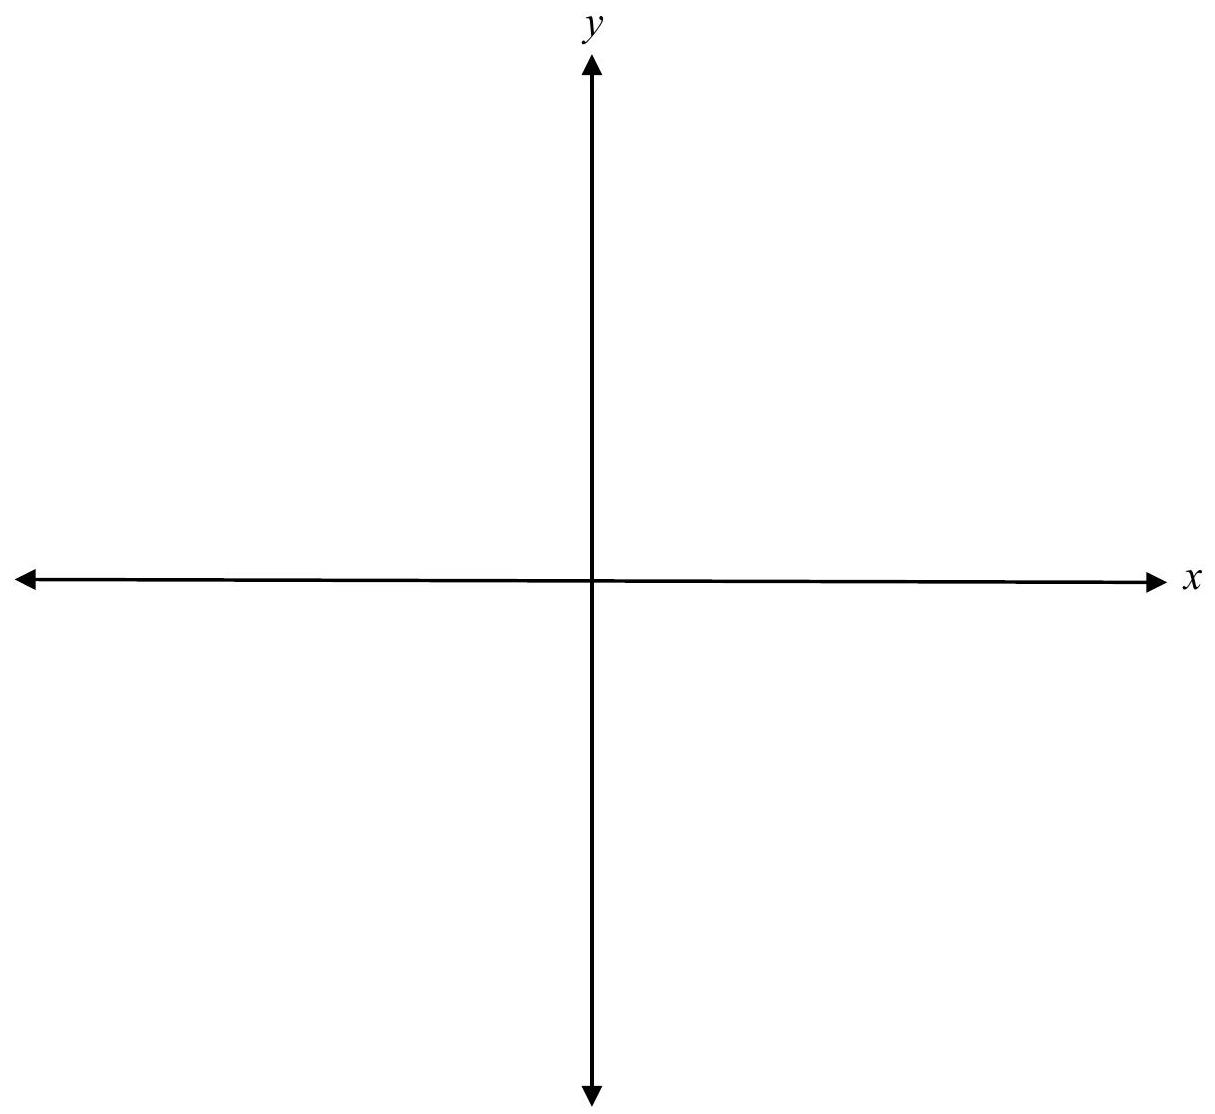
\includegraphics[max width=\textwidth, alt={}, center]{de5fb11a-28c7-4ac7-b7ff-0309cebac724-094_1114_1215_661_403}

If $f(x)=\frac{1}{x-2}$ and $g(x)=x-2$, what is the domain of $f(x) \cdot g(x)$ ?

Given $f(x)=(x+1)^{2}$ for $x \leq-1$, write the equation of $y=f^{-1}(x)$.

Sketch a graph of at least one period of the function $y=5 \sin [\pi(x+1)]$.\\
Clearly indicate the $x$-intercepts.\\
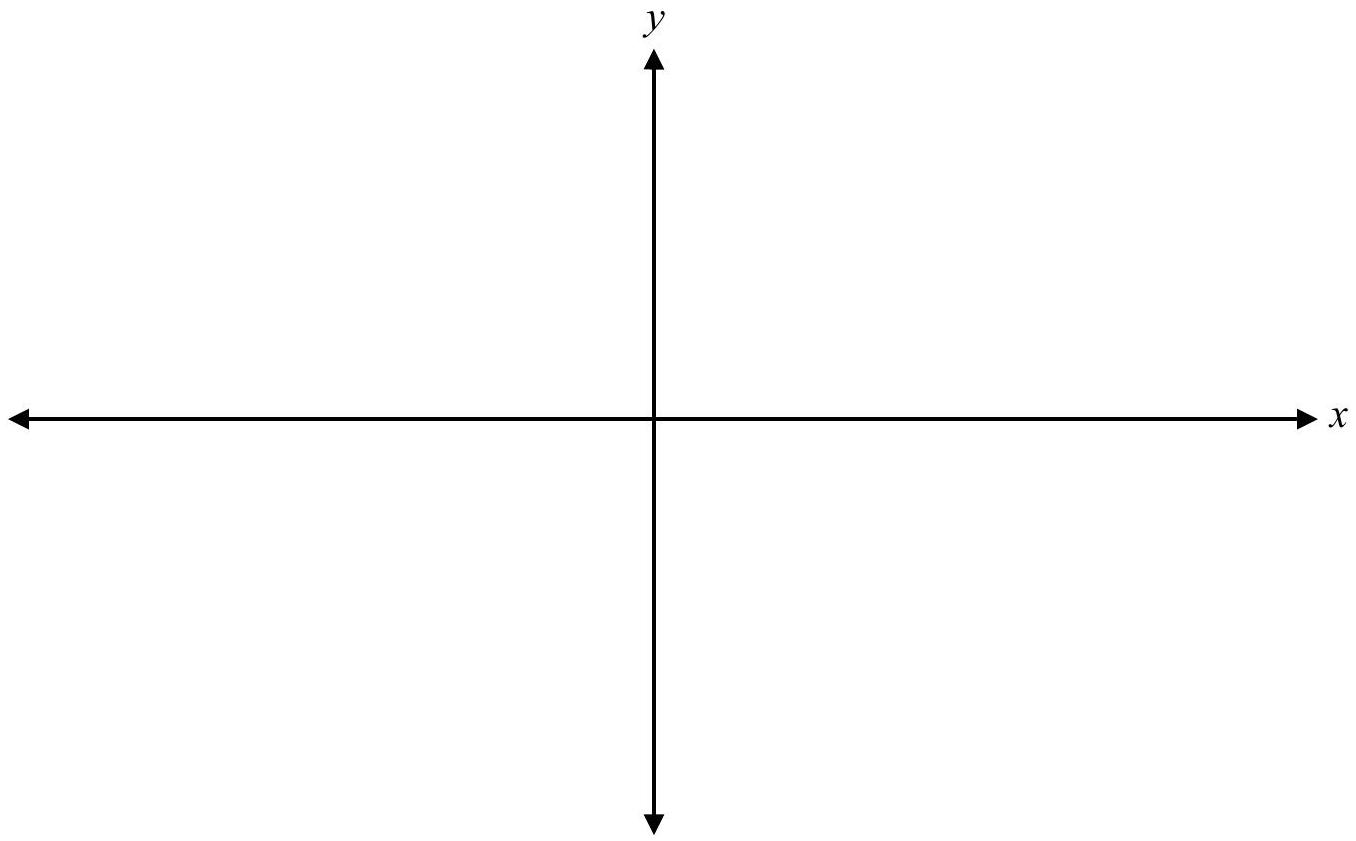
\includegraphics[max width=\textwidth, alt={}, center]{de5fb11a-28c7-4ac7-b7ff-0309cebac724-096_841_1356_693_378}

Sketch the graph of the following function:

$$
f(x)=\frac{x-2}{(2 x-3)(x-2)}
$$

\begin{center}
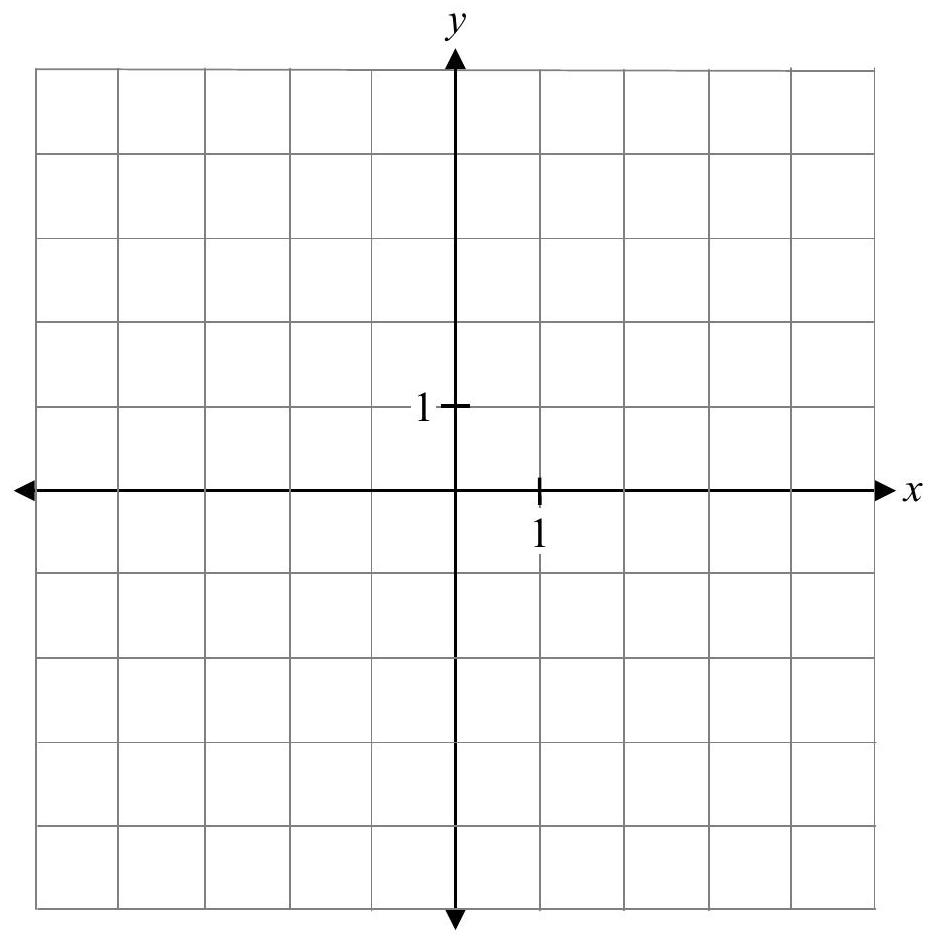
\includegraphics[max width=\textwidth, alt={}]{de5fb11a-28c7-4ac7-b7ff-0309cebac724-097_940_936_706_485}
\end{center}

Use the information in the diagram to determine the value of the arc length "s".\\
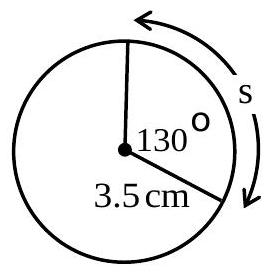
\includegraphics[max width=\textwidth, alt={}, center]{de5fb11a-28c7-4ac7-b7ff-0309cebac724-098_273_274_494_369}

Solve the following equation over the interval $[0,2 \pi)$.

$$
\tan ^{2} \theta+2.8 \tan \theta+1.96=0
$$

Use the quadratic formula $x=\frac{-b \pm \sqrt{b^{2}-4 a c}}{2 a}$ for $a x^{2}+b x+c=0$.

Determine how many monthly investments of $\$ 50$ would have to be deposited into a savings account that pays $3 \%$ annual interest, compounded monthly, for the account's future value to be $\$ 50,000$.\\
Use the formula:

$$
\mathrm{FV}=\frac{\mathrm{R}(1+i)^{n}-1}{i}
$$

where $\mathrm{FV}=$ the future value

$$
\begin{aligned}
\mathrm{R} & =\text { the investment amount } \\
i & =\frac{\text { the annual interest rate }}{\text { the number of compounding periods per year }} \\
n & =\text { the number of investments }
\end{aligned}
$$

Express your answer as a whole number.

There are 5 men and 4 women to be seated in a row.\\
How many arrangements are possible if two men must sit at the beginning of the row and two men must sit at the end of the row?

\section*{Question 5 D}
a) 3 marks\\
b) 2 marks\\
a) In the binomial expansion of $\frac{3}{x^{2}}-4 x^{5}$, determine the 3rd term.\\
b) In the binomial expansion of $\frac{3}{x^{2}}-4 x^{5}$, the 6th term contains $x^{25}$. Solve for $n$.

Given the following two functions, $f(x)=\sqrt{x-1}$ and $g(x)=x^{2}+1$, evaluate $g(f(3))$.

\section*{Question 7}
If $\theta$ terminates in quadrant II and $\csc \theta=\frac{3}{2}$, determine the exact value of $\tan \theta$.

\section*{Question 8}
a) 1 mark\\
b) 1 mark\\
a) Determine the remainder when $x^{4}-3 x^{2}+1$ is divided by $x+2$.\\
b) Is $x+2$ a factor of $x^{4}-3 x^{2}+1$ ?

Explain your reasoning.

Given the graph of $y=f(x)$ below, sketch the graph of $y=2 f(x)-3$.\\
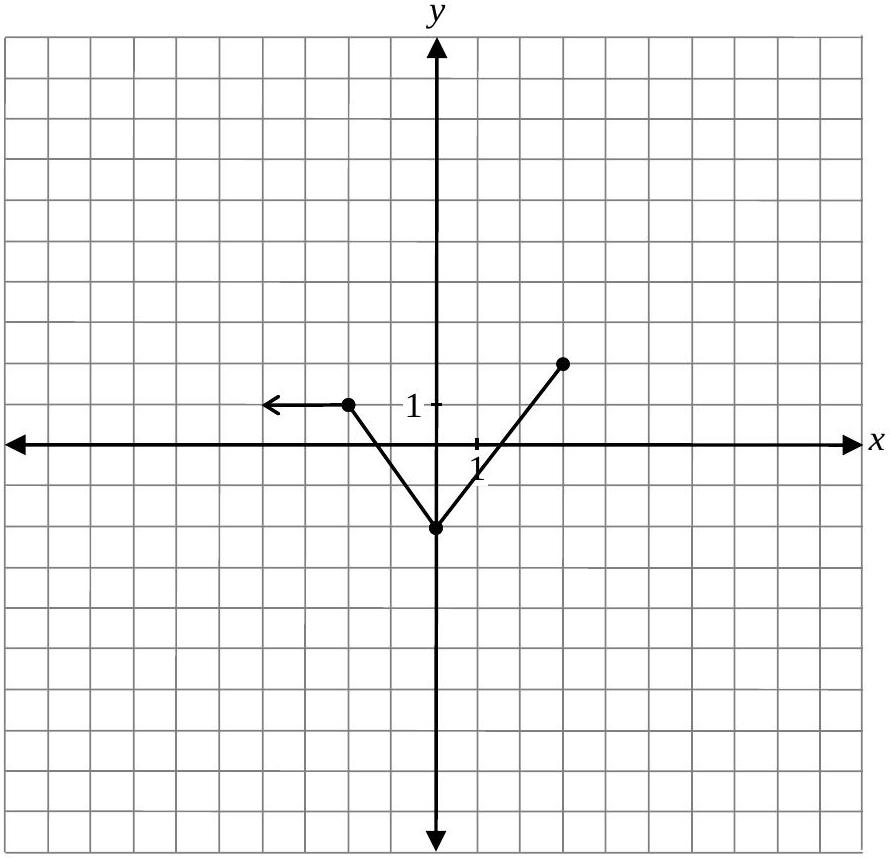
\includegraphics[max width=\textwidth, alt={}, center]{de5fb11a-28c7-4ac7-b7ff-0309cebac724-105_858_890_468_380}\\
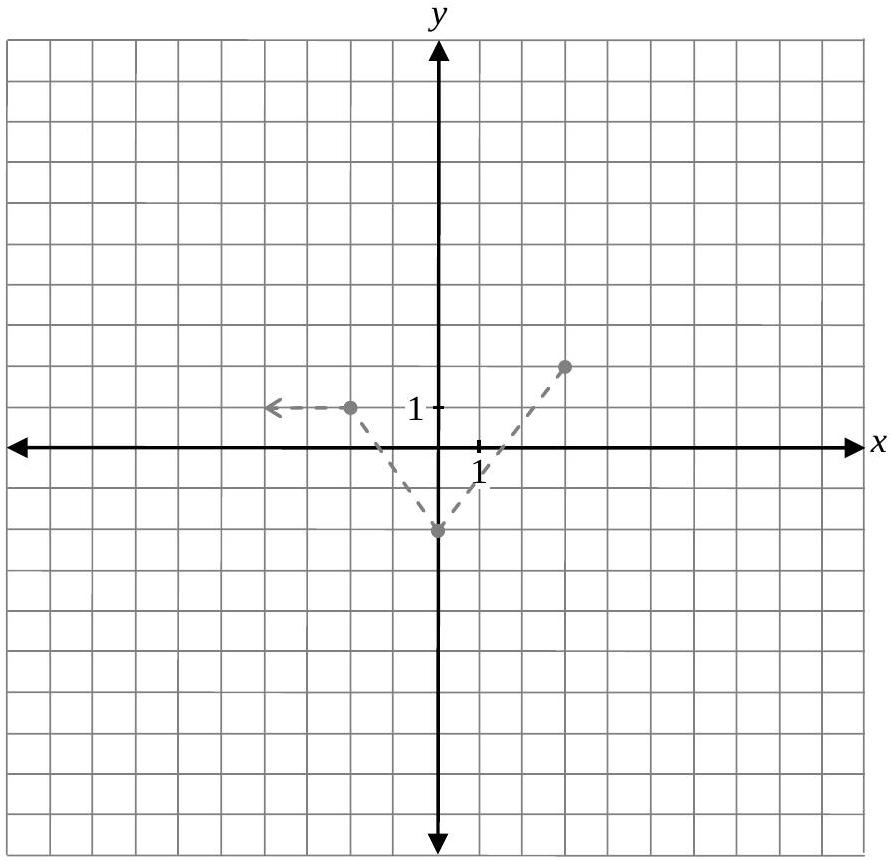
\includegraphics[max width=\textwidth, alt={}, center]{de5fb11a-28c7-4ac7-b7ff-0309cebac724-105_862_892_1495_378}

The graph of $f(x)$ has already been drawn for your reference.

No marks will be awarded for the graph of $f(x)$.

Determine one possible restriction for the domain of $f(x)=(x-1)^{2}$ so that the inverse of $f(x)$ is a function.

\section*{Question 11}
Using the graph of the sinusoidal function below, find the value of $y$ in the point $(6, y)$.\\
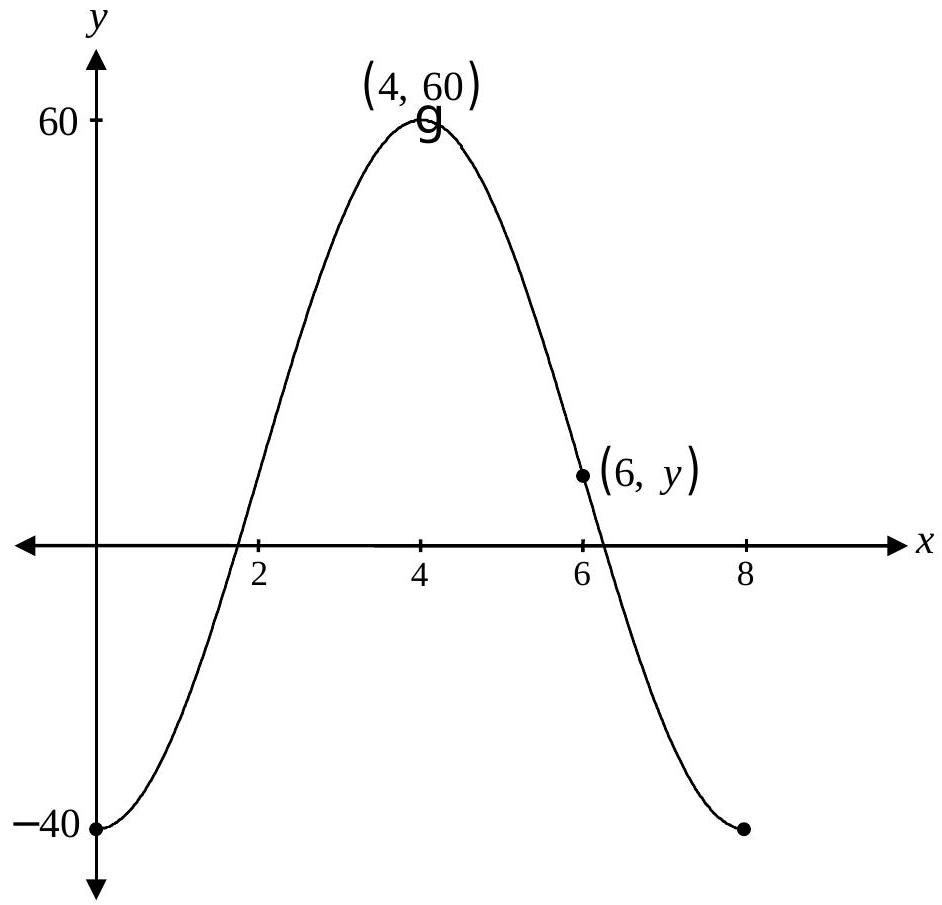
\includegraphics[max width=\textwidth, alt={}, center]{de5fb11a-28c7-4ac7-b7ff-0309cebac724-106_905_942_1480_268}

Billy was given the graph of $y=f(x)$.\\
He was asked to sketch the graph of $y=\sqrt{f(x)}$.\\
His answer is given on the graph below.\\
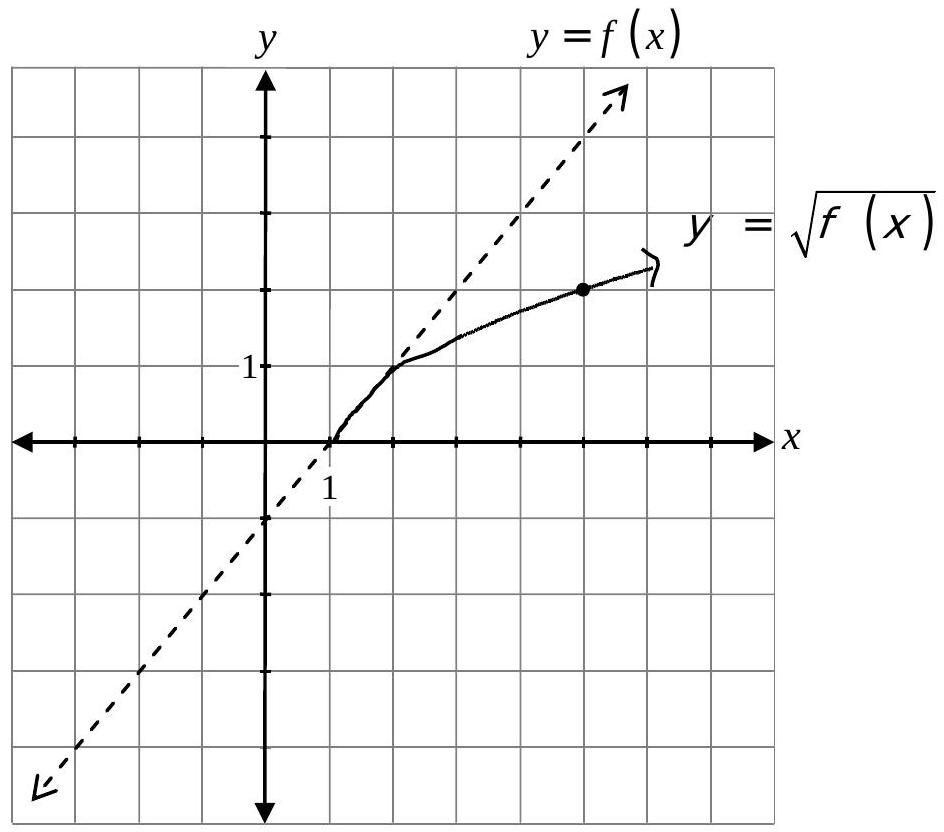
\includegraphics[max width=\textwidth, alt={}, center]{de5fb11a-28c7-4ac7-b7ff-0309cebac724-107_832_944_586_406}

Explain the error Billy made when sketching the graph of $y=\sqrt{f(x)}$.

Explain why a locker combination should really be called a locker permutation.\\
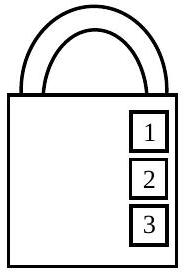
\includegraphics[max width=\textwidth, alt={}, center]{de5fb11a-28c7-4ac7-b7ff-0309cebac724-108_274_184_352_1641}

The graph of $f(x)=x^{2}+4$ is reflected over the $x$-axis.\\
Write the equation of the new function.

$$
y=
$$

Given the graph of $y=f(x)$ below,\\
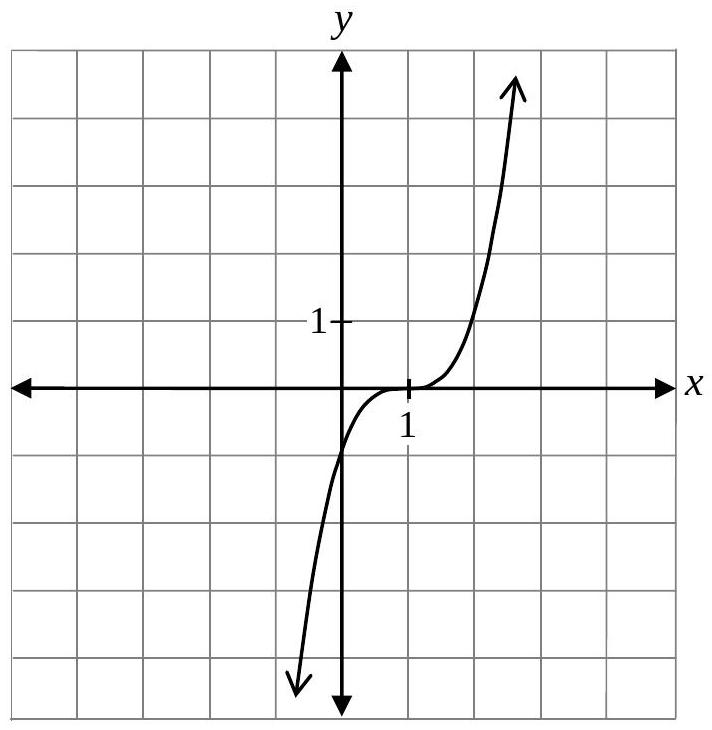
\includegraphics[max width=\textwidth, alt={}, center]{de5fb11a-28c7-4ac7-b7ff-0309cebac724-109_730_712_459_586}\\
sketch the graph of $y=\frac{1}{f(x)}$.\\
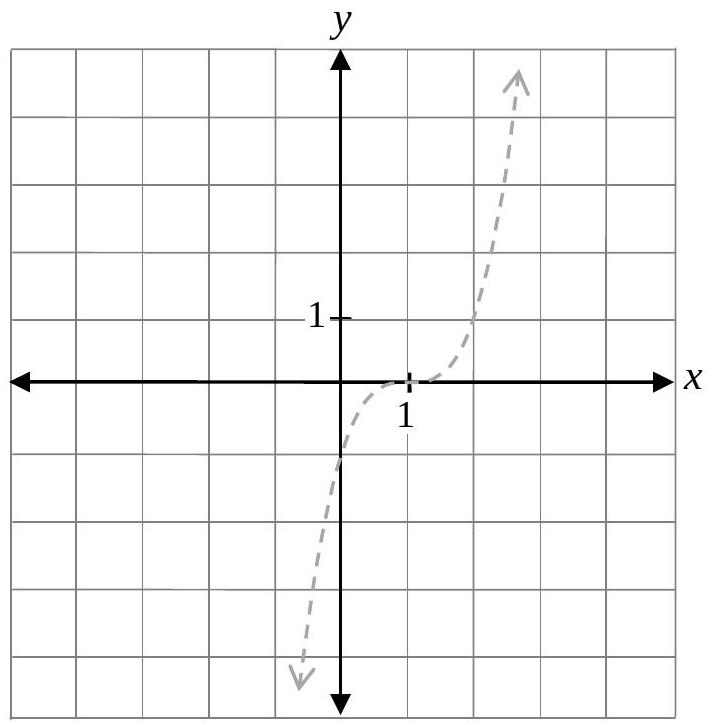
\includegraphics[max width=\textwidth, alt={}, center]{de5fb11a-28c7-4ac7-b7ff-0309cebac724-109_725_712_1454_573}

The graph of $f(x)$ has already been drawn for your reference.

No marks will be awarded for the graph of $f(x)$.

Divide $\left(x^{3}-5 x-4\right)$ by $(x+1)$.

You are given the following row of Pascal’s Triangle.

\begin{center}
\begin{tabular}{llllllll}
1 & 7 & 21 & 35 & 35 & 21 & 7 & 1 \\
\end{tabular}
\end{center}

Determine the values of the next row.

Given the graph of $y=f(x)$ below, state the domain and range of $y=\sqrt{f(x)}$.\\
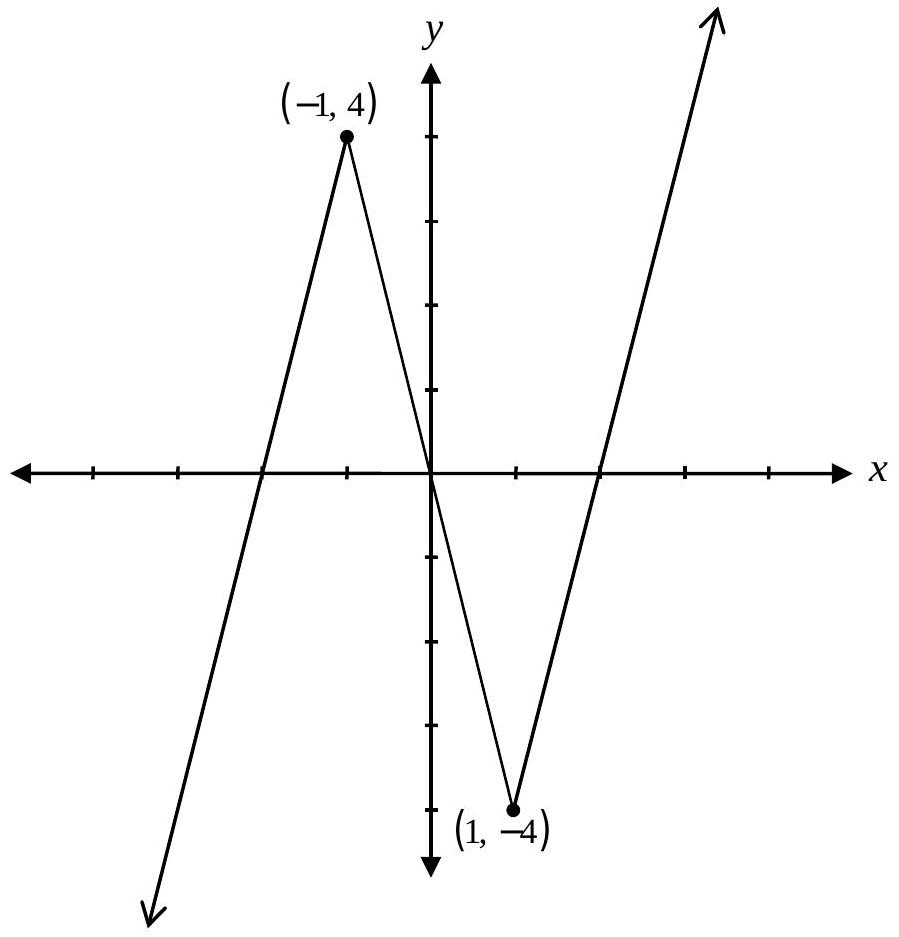
\includegraphics[max width=\textwidth, alt={}, center]{de5fb11a-28c7-4ac7-b7ff-0309cebac724-111_937_899_466_281}

Domain: $\_\_\_\_$\\
Range: $\_\_\_\_$

Prove the identity below for all permissible values of $\theta$ :

$$
\frac{1-\tan ^{2} \theta}{1+\tan ^{2} \theta}=\cos 2 \theta
$$

\begin{center}
\begin{tabular}{|l|l|}
\hline
Left-Hand Side & Right-Hand Side \\
\hline
 &  \\
\hline
\end{tabular}
\end{center}

Given the graph of the function of $f(x)$ below, what is the range of $y=|f(x)|$ ?\\
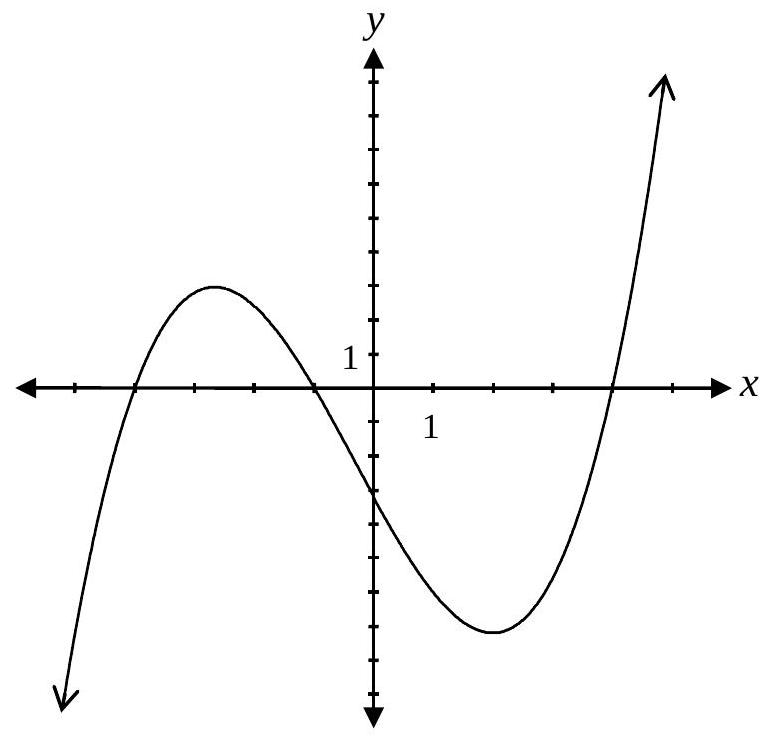
\includegraphics[max width=\textwidth, alt={}, center]{de5fb11a-28c7-4ac7-b7ff-0309cebac724-113_740_771_457_577}\\
a) $y \in^{\circ}$\\
b) $y \geq-7$\\
c) $y \geq 0$\\
d) $-4 \leq y \leq-1$ or $y \geq 4$

\section*{Question 21}
Simplify the following expression:

$$
\frac{1}{2} \log _{a} 36-\log _{a} 2
$$

a) $\log _{a} 3$\\
b) $\log _{a} 4$\\
c) $\log _{a} 9$\\
d) $\log _{a} 12$

Given $f(x)=x^{2}-x+2$, an equation that represents the graph of $f(x)$ shifted 3 units to the right is:\\
a) $y=(x+3)^{2}-(x+3)-3$\\
b) $y=(x-3)^{2}-(x-3)+2$\\
c) $y=(x-3)^{2}-x-2$\\
d) $y=x^{2}-x+2-3$

\section*{Question 23}
What is the domain of the function $y=\sqrt{-4 x}$ ?\\
a) $\left\{x \in^{\circ} \mid x \geq 2\right\}$\\
b) $\left\{x \in^{\circ} \mid x \leq 2\right\}$\\
c) $\left\{x \in^{\circ} \mid x \geq 0\right\}$\\
d) $\left\{x \in^{\circ} \mid x \leq 0\right\}$

\section*{Question 24}
Which of the following is true about the two functions below?

$$
f(x)=\frac{(x+2)(x-2)}{x-2} \quad g(x)=\frac{(x-2)(x+1)}{(x+2)(x-2)}
$$

a) Both have a point of discontinuity (hole) when $x=2$.\\
b) Both have the same vertical asymptote.\\
c) Both have the same horizontal asymptote.\\
d) Both have the same $y$-intercept.

The general solution to the equation $\cos \theta=-\frac{1}{2}$ is:\\
a) $\begin{array}{ll}\theta= & \frac{\pi}{3}+2 \pi k \\ 5 \pi & \text { where } k \in I\end{array}$

$$
\theta=\frac{5 \pi}{3}+2 \pi k
$$

b) $\theta=\frac{\pi}{3}+\pi k \quad$ where $k \in \mathrm{I}$

$$
\theta=\frac{5 \pi}{3}+\pi k
$$

c) $\theta=\frac{2 \pi}{3}+2 \pi k \quad$ where $k \in \mathrm{I}$

$$
\theta=\frac{4 \pi}{3}+2 \pi k
$$

d) $\theta=\frac{2 \pi}{3}+\pi k \quad$ where $k \in \mathrm{I}$

$$
\theta=\frac{4 \pi}{3}+\pi k
$$

\section*{Question 26}
If the equation $y=\sin (b(x+\pi))$ is represented by the following graph, what is the value of $b$ ?\\
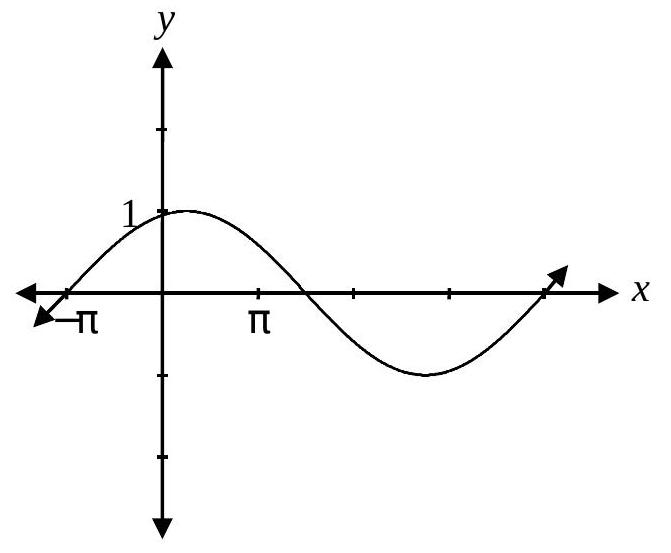
\includegraphics[max width=\textwidth, alt={}, center]{de5fb11a-28c7-4ac7-b7ff-0309cebac724-115_553_671_1858_797}\\
a) $\frac{2}{5}$\\
b) $\frac{5}{2}$\\
c) $\frac{2 \pi}{5}$\\
d) $5 \pi$

Which of the following is closest to the value of $\log _{2} 40+\log _{5} 125$ ?\\
a) 3\\
b) 8\\
c) 10\\
d) 45

Question 28

A sheet of paper 12 cm long and 8 cm wide is used to make a box with no lid. Equal squares of side length $x \mathrm{~cm}$ are cut from each of the corners and the sides are folded up to make the box.\\
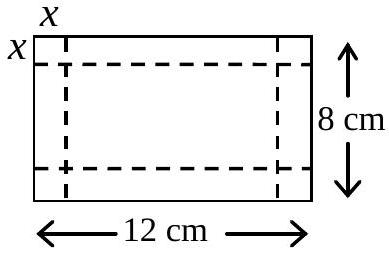
\includegraphics[max width=\textwidth, alt={}, center]{de5fb11a-28c7-4ac7-b7ff-0309cebac724-116_253_389_936_305}

Which of the following expresses the volume of the box?\\
a) $\mathrm{V}(x)=x(12+x)(8+x)$\\
b) $\mathrm{V}(x)=x(12-x)(8-x)$\\
c) $\mathrm{V}(x)=x(12+2 x)(8+2 x)$\\
d) $\mathrm{V}(x)=x(12-2 x)(8-2 x)$

Given that the graph of $f(x)$ contains the point $(-3,5)$, what point must be on the graph of $f(-x)$ ?\\
a) $(-3,-5)$\\
b) $(3,5)$\\
c) $(3,-5)$\\
d) $(5,-3)$

Determine one positive and one negative coterminal angle with the angle $\frac{5 \pi}{6}$.

Evaluate:

$$
\sin \frac{11 \pi}{3} \quad \sec \frac{11 \pi}{6}
$$

Given the equation $2 \sin ^{2} \theta-3 \sin \theta+1=0$, verify that $\theta=\frac{\pi}{2}$ is a solution.

\section*{Question 33}
Using the laws of logarithms, expand:

$$
\log _{a} \frac{x g y}{z}
$$

a) Sketch the graph of $f(x)=3^{x}+1$.\\
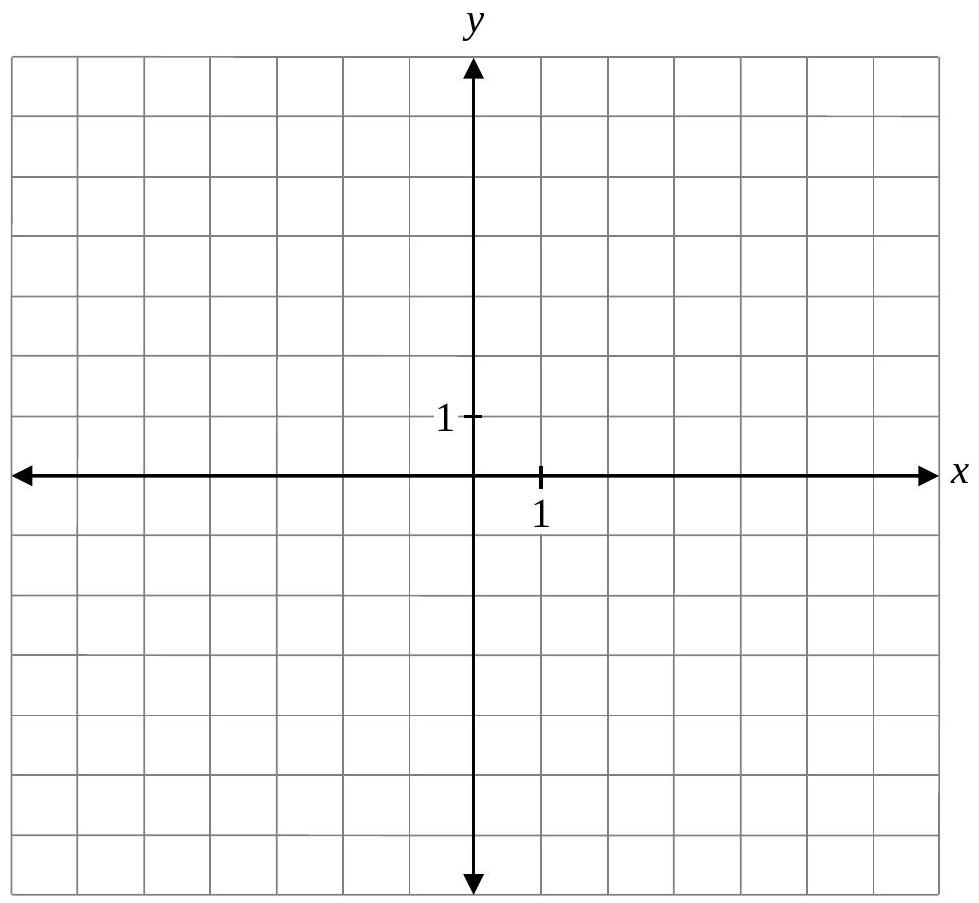
\includegraphics[max width=\textwidth, alt={}, center]{de5fb11a-28c7-4ac7-b7ff-0309cebac724-119_903_979_485_455}\\
b) Sketch the graph of $f^{-1}(x)$.\\
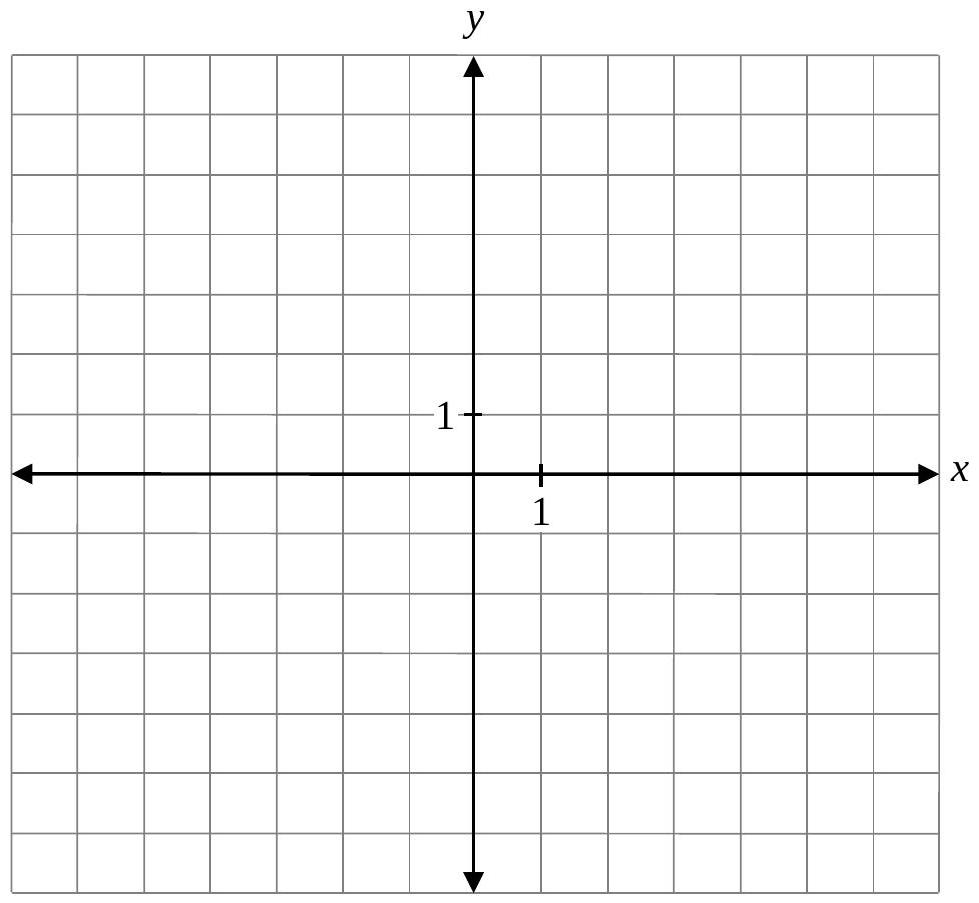
\includegraphics[max width=\textwidth, alt={}, center]{de5fb11a-28c7-4ac7-b7ff-0309cebac724-119_903_979_1600_455}

Determine the $x$-intercept and $y$-intercept of $y=\log _{2}(x+4)-1$.

Explain the error that was made when solving the following equation:

$$
\sin 2 \theta=\cos \theta, \text { where } \theta \in^{\circ}
$$

$$
\begin{aligned}
& \sin 2 \theta=\cos \theta \\
& 2 \sin \theta \cos \theta=\cos \theta \\
& \frac{2 \sin \theta \cos \theta}{\cos \theta}=\frac{\cos \theta}{\cos \theta} \\
& 2 \sin \theta=1 \\
& \sin \theta=\frac{1}{2} \\
& \theta=\frac{\pi}{6}+2 k \pi, \frac{5 \pi}{6}+2 k \pi, k \in I
\end{aligned}
$$

Given $f(x)=x^{2}-2 x-3$ and $g(x)=x+1$ :\\
a) Write the equation of $y=f(g(x))$.\\
b) Sketch the graph of $y=f(g(x))$.\\
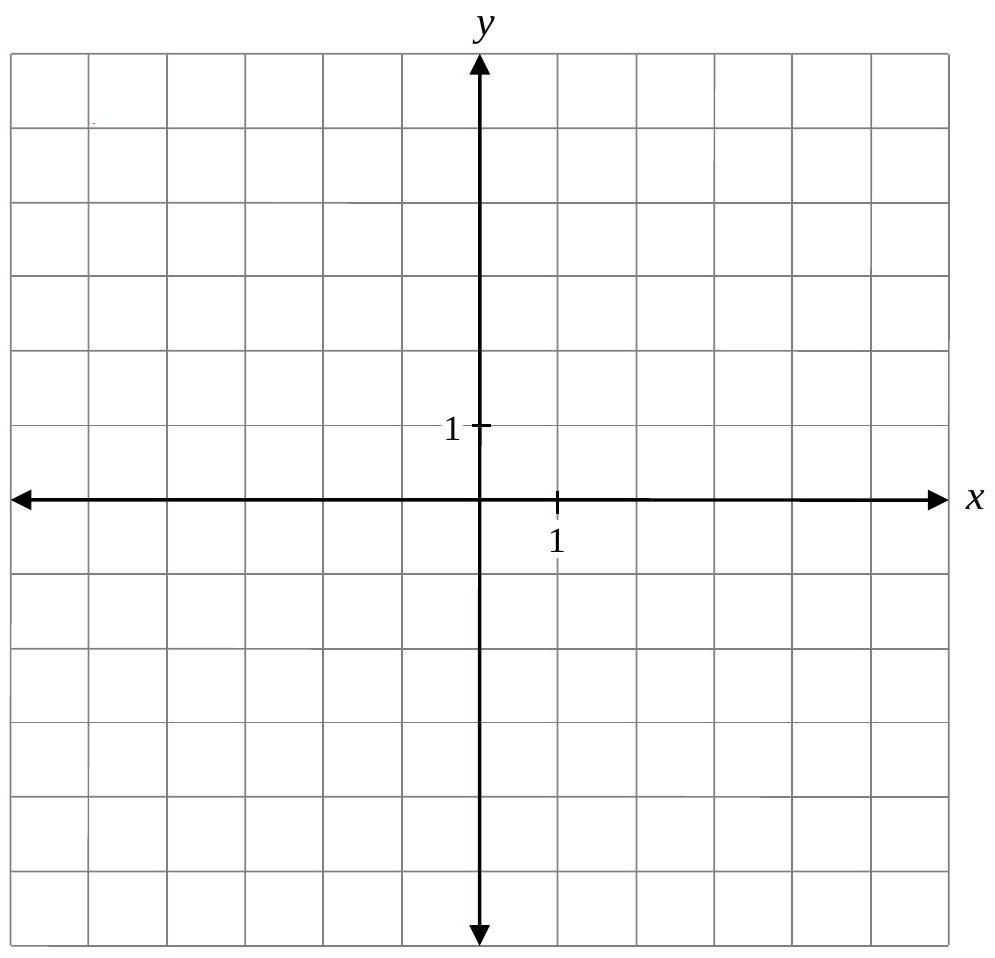
\includegraphics[max width=\textwidth, alt={}, center]{de5fb11a-28c7-4ac7-b7ff-0309cebac724-121_958_995_1576_537}

Is the point $\frac{3}{4},-\frac{\sqrt{3}}{4}$ on the unit circle?\\
Justify your answer.

\section*{Question 39}
Explain why the equation $\sec \theta=\frac{1}{4}$ has no solution.

The graph of $y=\sin 2 x$ is sketched below.\\
Explain how to use this graph to solve the equation $\sin 2 x=\frac{1}{2}$ over the interval $[0,2 \pi]$.\\
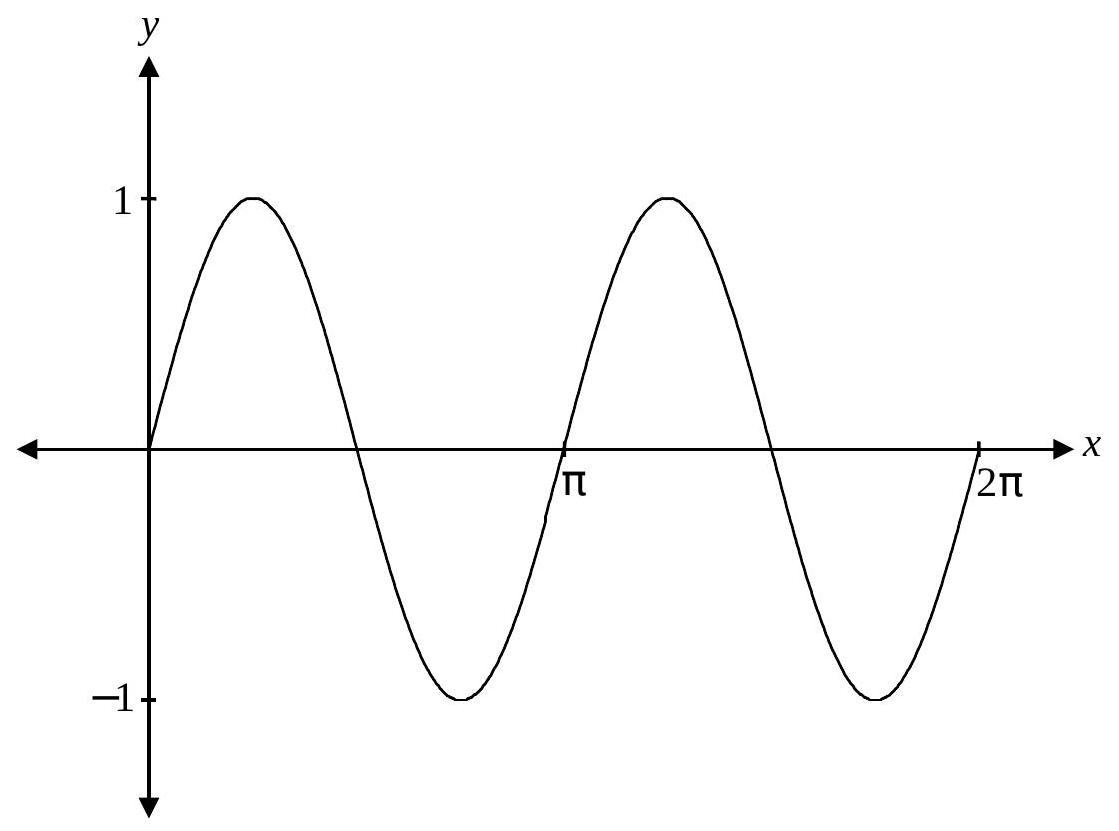
\includegraphics[max width=\textwidth, alt={}, center]{de5fb11a-28c7-4ac7-b7ff-0309cebac724-123_831_1119_575_433}

Sketch the graph of $y=-4 \cos (2 x)$ over the interval $[-\pi, \pi]$.\\
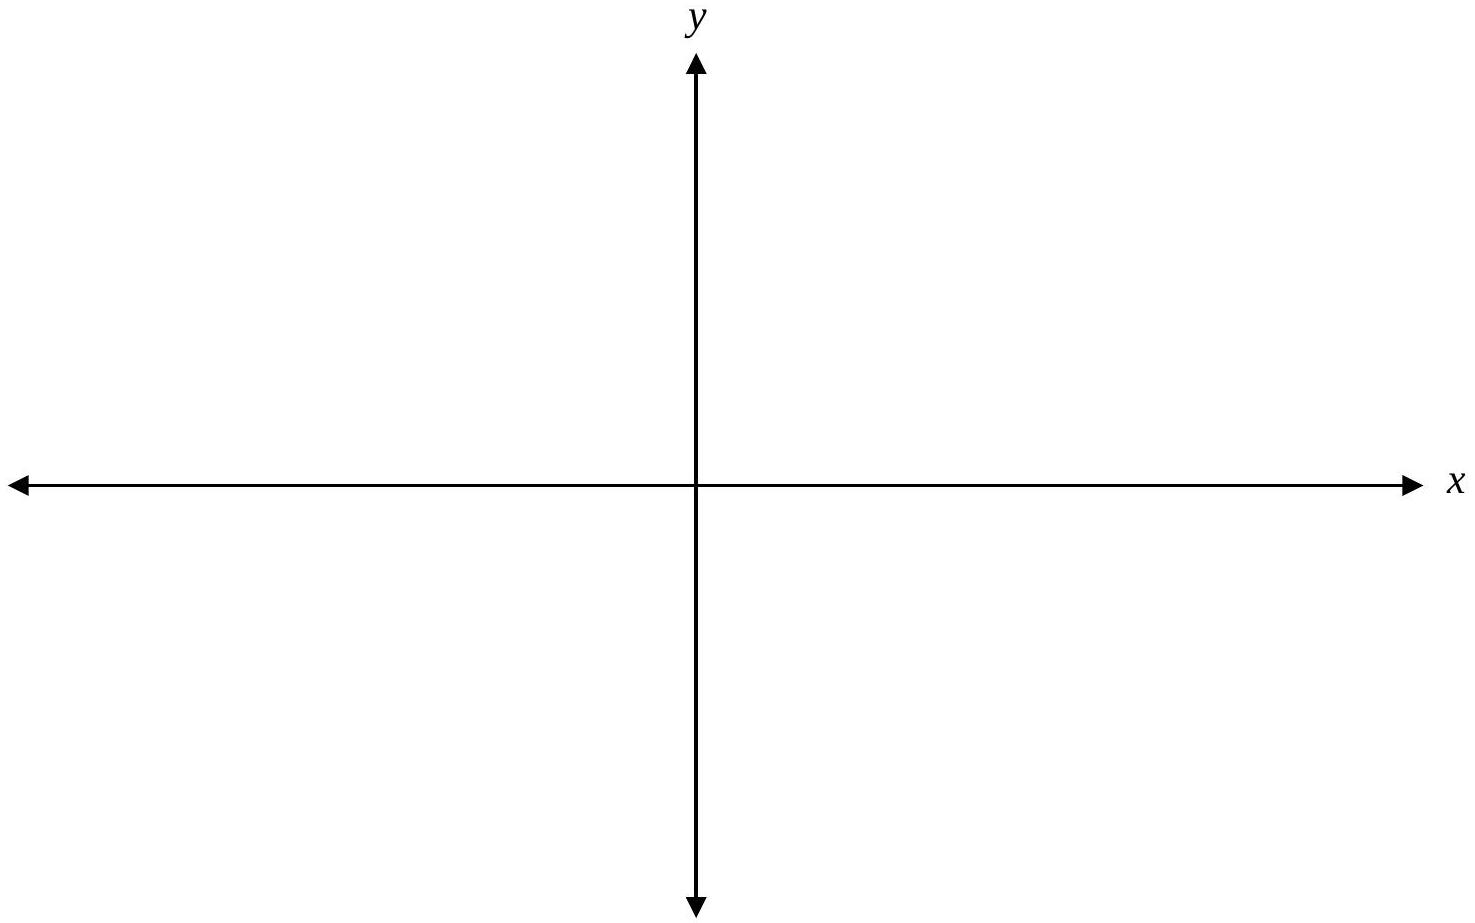
\includegraphics[max width=\textwidth, alt={}, center]{de5fb11a-28c7-4ac7-b7ff-0309cebac724-124_923_1475_515_251}

Write the equation for $f(x)$ that satisfies all of the following conditions:

\begin{itemize}
  \item $f(x)$ is a polynomial function of degree 4
  \item $f(x)$ has a zero at 2 with a multiplicity of 3
  \item $f(x)$ has a zero at -5
  \item $f(x)$ has a $y$-intercept of 80
\end{itemize}

Find the exact value of $\sin \frac{19 \pi}{12}$.

Solve the following equation:

$$
2 \log _{2}(x-1)-\log _{2}(x-5)=\log _{2}(x+1)
$$

Sketch the graph of $f(x)=(x-1)^{2}(x+2)^{3}$.\\
Label the $x$-intercepts and the $y$-intercept.\\
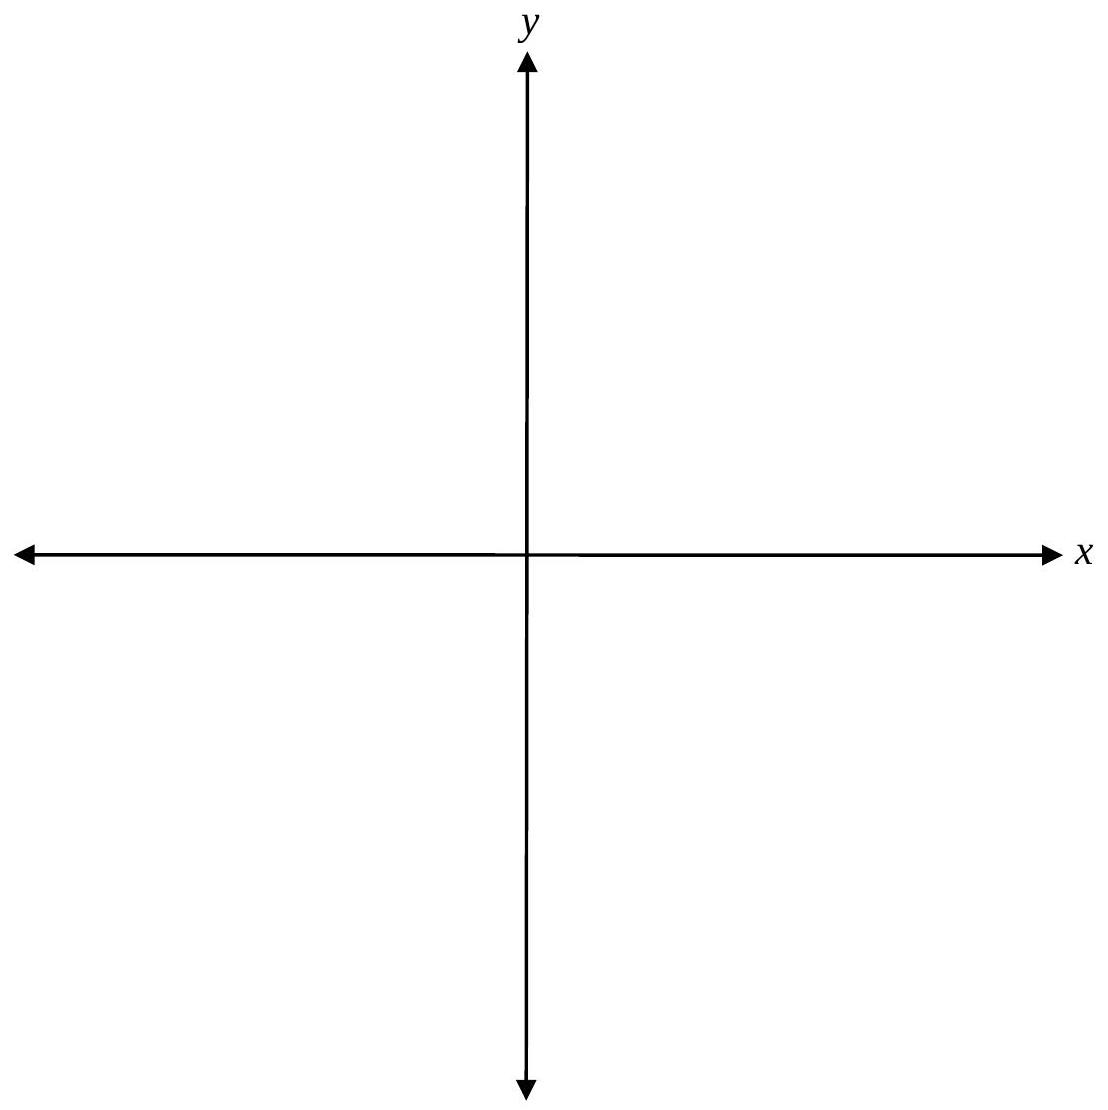
\includegraphics[max width=\textwidth, alt={}, center]{de5fb11a-28c7-4ac7-b7ff-0309cebac724-128_1110_1108_620_433}

Sketch the graph of $y=-\sqrt{3(x+1)}$.\\
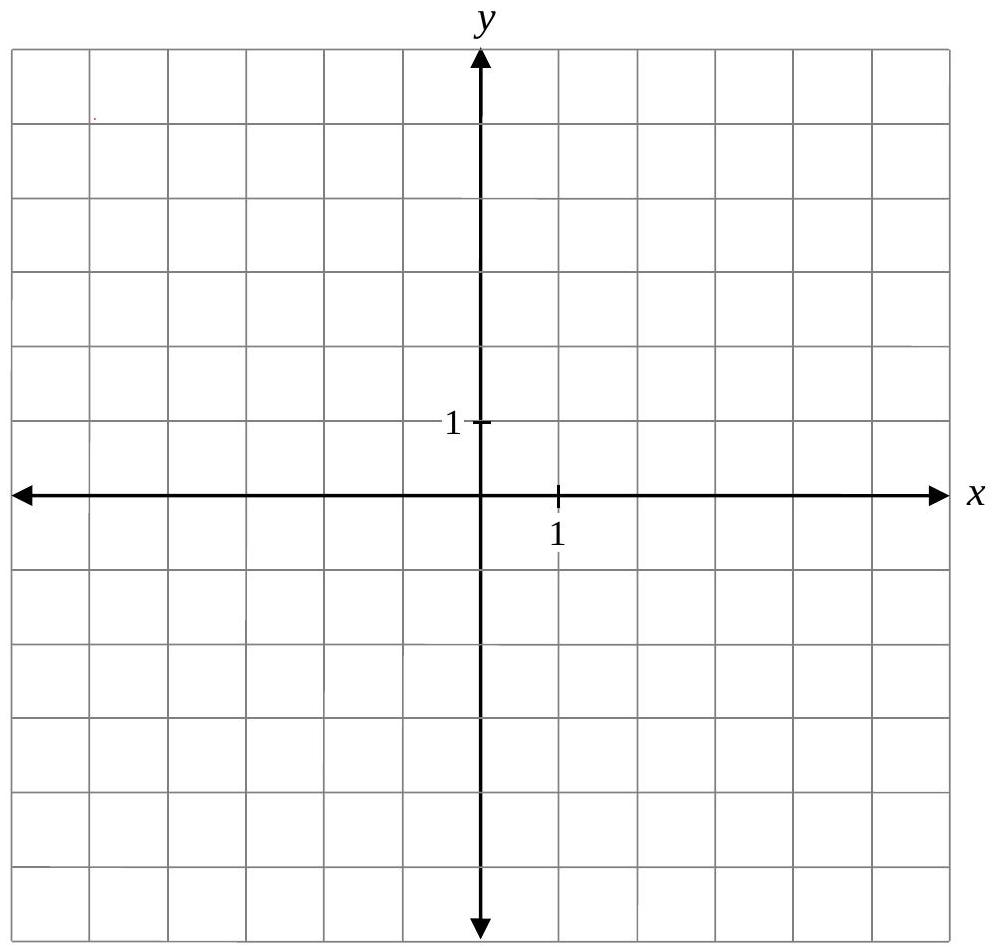
\includegraphics[max width=\textwidth, alt={}, center]{de5fb11a-28c7-4ac7-b7ff-0309cebac724-129_949_993_519_522}

Solve:

$$
{ }_{n-1} P_{2}=42
$$

Sketch the graph of $y=\frac{2 x}{x+2}$.\\
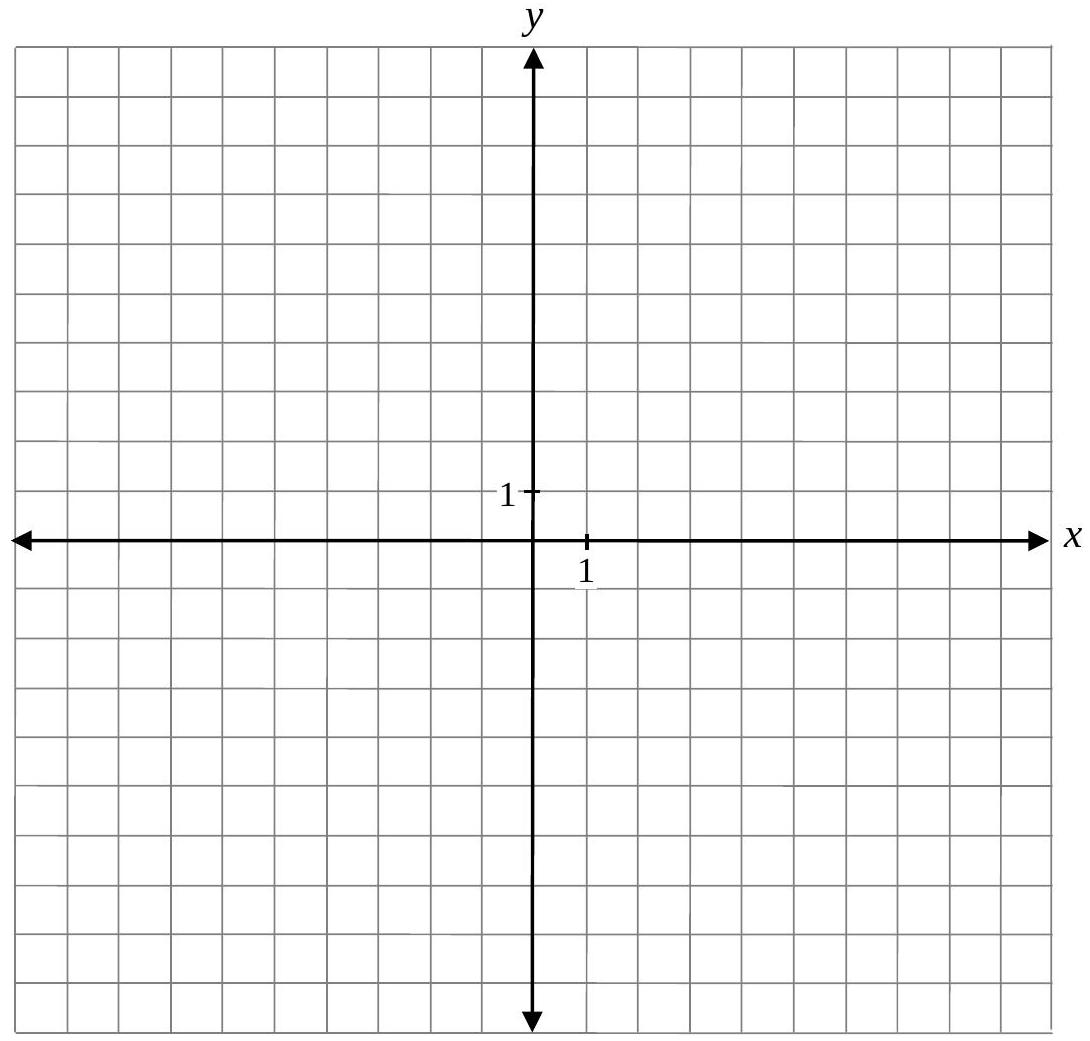
\includegraphics[max width=\textwidth, alt={}, center]{de5fb11a-28c7-4ac7-b7ff-0309cebac724-131_1041_1090_605_541}

Given the graphs of $f(x)$ and $g(x)$, sketch the graph of $(f g g)(x)$.\\
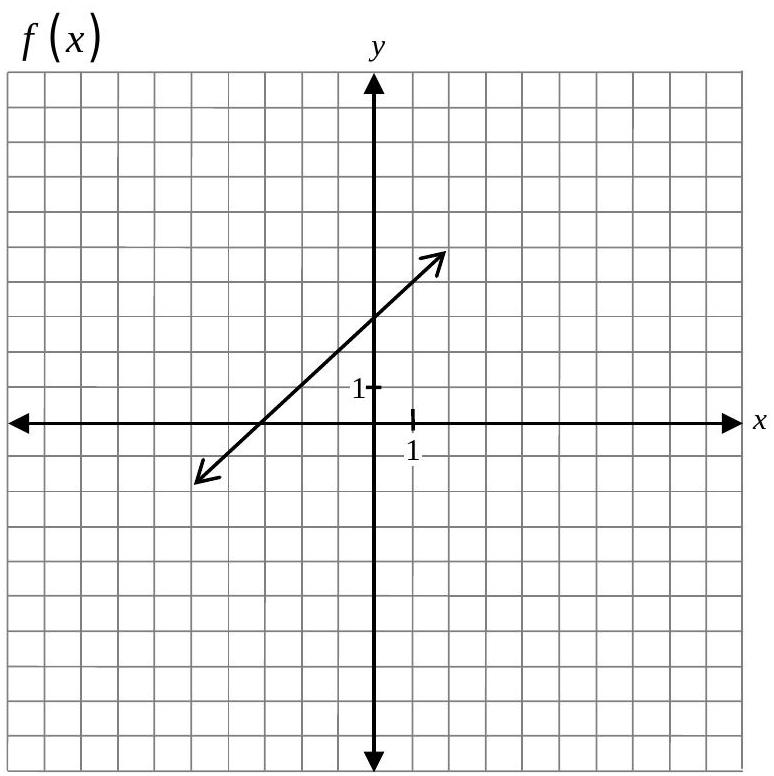
\includegraphics[max width=\textwidth, alt={}, center]{de5fb11a-28c7-4ac7-b7ff-0309cebac724-132_776_774_507_277}\\
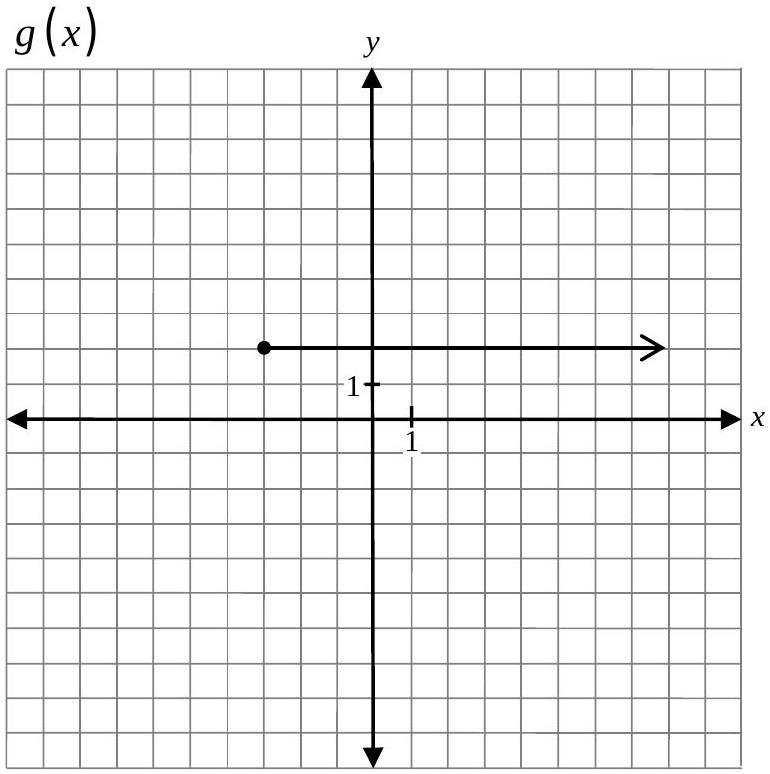
\includegraphics[max width=\textwidth, alt={}, center]{de5fb11a-28c7-4ac7-b7ff-0309cebac724-132_774_770_507_1153}\\
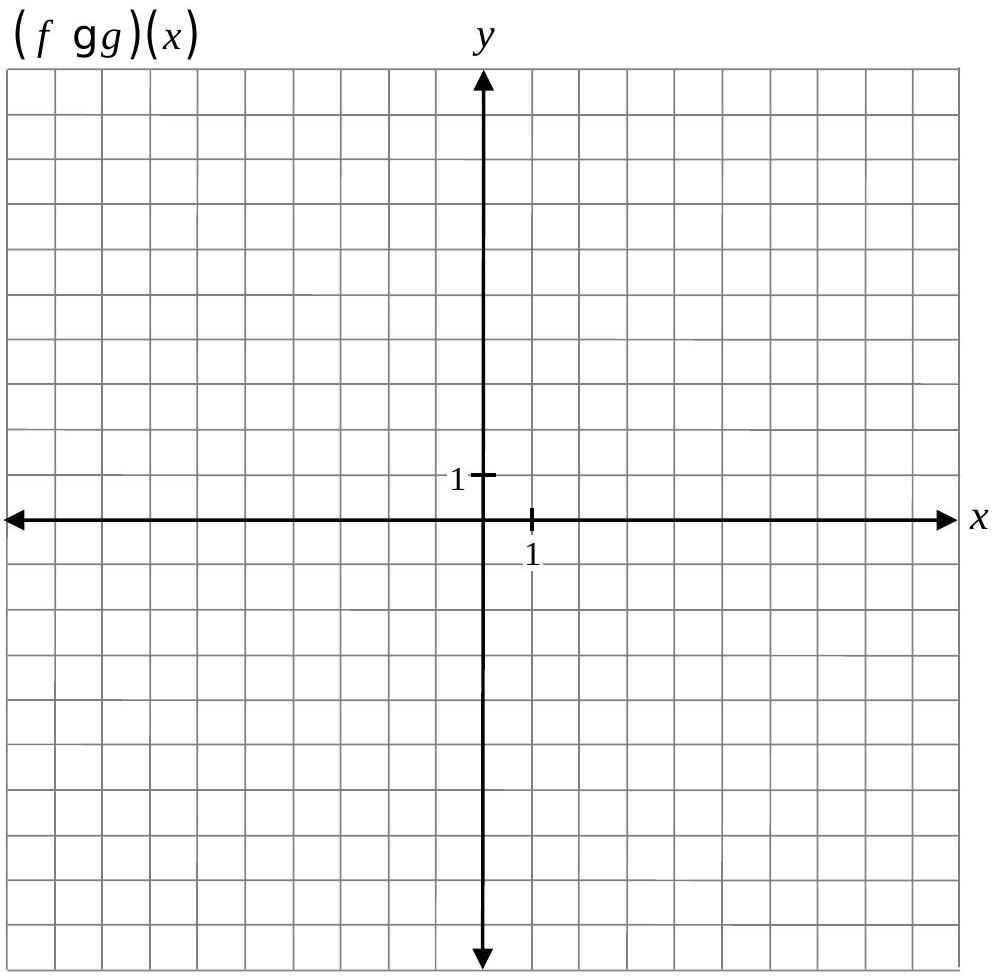
\includegraphics[max width=\textwidth, alt={}, center]{de5fb11a-28c7-4ac7-b7ff-0309cebac724-132_979_996_1469_584}

Convert $-\frac{13 \pi}{5}$ to degrees.\\
a) 1 mark\\
b) 1 mark\\
c) 1 mark\\
a) From a group of 9 people, in how many ways can you select a committee of 4 members?\\
b) From a group of 9 people, in how many ways can you select a president, a vice president, a secretary, and a treasurer?\\
c) Explain why the answers in a) and b) are different.

A population of 500 bacteria will triple in 20 hours.\\
Using the formula given below,\\
$A=P e^{r t}$\\
$A=$ population after $t$ hours\\
$P=$ initial population\\
$r=$ rate of growth\\
$t=$ time in hours\\
a) Determine the rate of growth, $r$.\\
b) Determine how many hours it will take for the initial population to double with the same rate of growth.

Talla incorrectly solved the following trigonometric equation:\\
Solve: $2 \sec x-5=0 ; 0^{\circ} \leq x \leq 360^{\circ}$.\\
Talla's work:\\
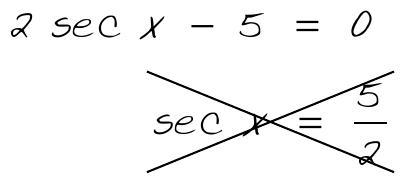
\includegraphics[max width=\textwidth, alt={}, center]{de5fb11a-28c7-4ac7-b7ff-0309cebac724-136_180_408_592_592}

No solution, sec $x$ cannot be greater than 1 .\\
a) Explain her error.\\
b) Determine the correct solution.

Simplify the 6th term in the expansion of:

$$
\left(2 x-\frac{3}{x^{2}}\right)^{10}
$$

Determine the arc length subtended by a central angle if the diameter is 19 cm and the central angle is 1.6 radians.

Solve the following equation algebraically for $x$, where $0 \leq x \leq 2 \pi$.

$$
2 \cos ^{2} x=-3 \sin x
$$

In how many different ways can you arrange the letters in the word VOLLEYBALL? State your answer as a factorial.

Is $(x-2)$ a factor of the polynomial $p(x)=-x^{4}-3 x^{3}+11 x^{2}+3 x-10$ ?\\
Justify your response.

Determine the period of the sinusoidal function $y=\frac{1}{2} \sin \left(\frac{1}{3} x\right)$.\\
State your answer in radians.

The domain of $f(x)$ is $x \leq 2$. The domain of $g(x)$ is $x \geq-7$.\\
State the domain of $f(x)+g(x)$.\\
Justify your answer.

Prove the identity below for all permissible values of $\theta$.

$$
\frac{1}{1+\cos \theta}=\csc ^{2} \theta-\frac{\cot \theta}{\sin \theta}
$$

\begin{center}
\begin{tabular}{|l|l|}
\hline
Left-Hand Side & Right-Hand Side \\
\hline
\end{tabular}
\end{center}

Explain how the end behaviours of the graphs of polynomial functions with an even degree and with an odd degree are different.

Given the graphs of $f(x)$ and $g(x)$, sketch the graph of $g(x)-f(x)$.

\begin{figure}[h]
\begin{center}
\captionsetup{labelformat=empty}
\caption{$f(x)$}
  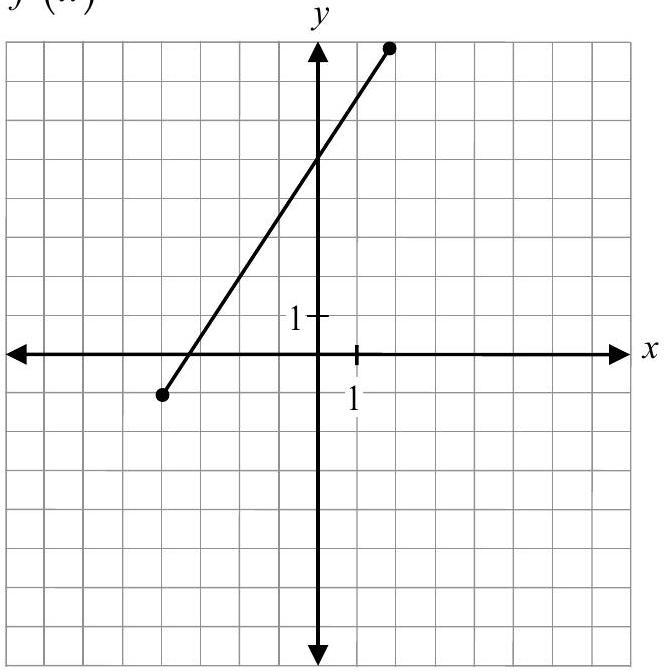
\includegraphics[alt={},max width=\textwidth]{de5fb11a-28c7-4ac7-b7ff-0309cebac724-146_671_665_526_279}
\end{center}
\end{figure}

\begin{figure}[h]
\begin{center}
\captionsetup{labelformat=empty}
\caption{$g(x)$}
  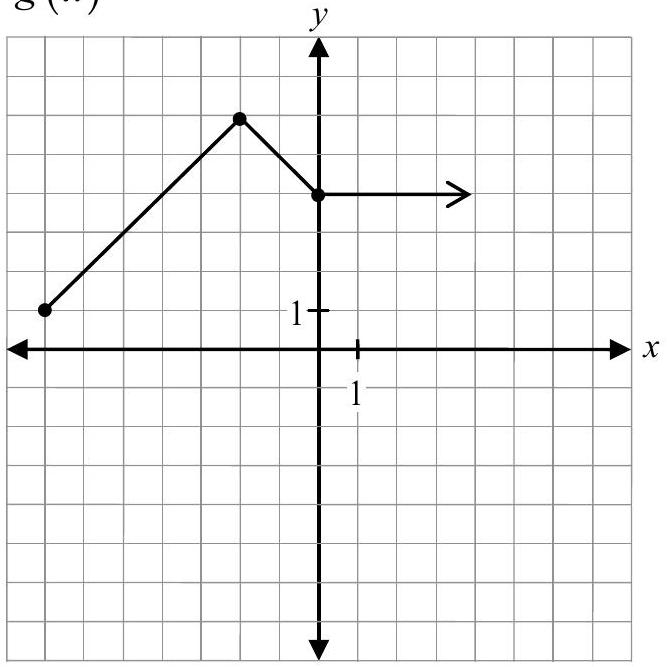
\includegraphics[alt={},max width=\textwidth]{de5fb11a-28c7-4ac7-b7ff-0309cebac724-146_667_667_526_1102}
\end{center}
\end{figure}

$$
g(x)-f(x)
$$

\begin{center}
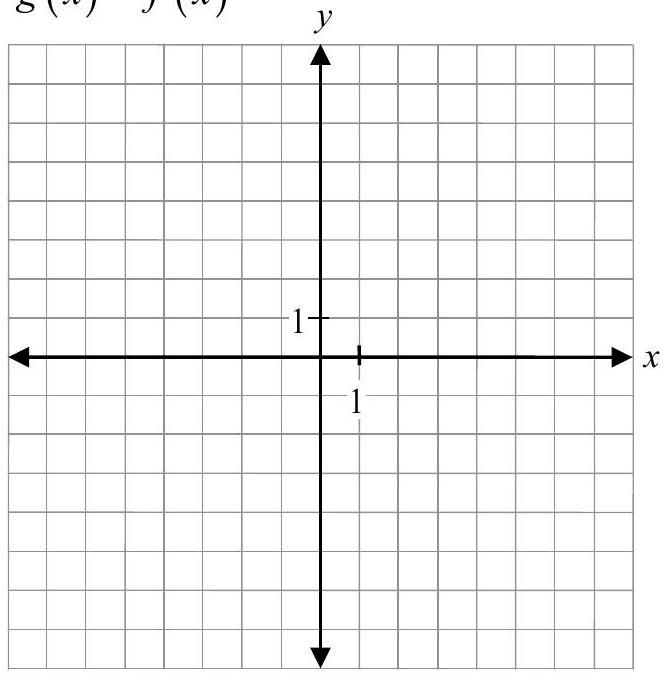
\includegraphics[max width=\textwidth, alt={}]{de5fb11a-28c7-4ac7-b7ff-0309cebac724-146_673_665_1366_708}
\end{center}

Given $f(x)=-3 x+7$, evaluate $f^{-1}(-2)$.

How many terms are there in the expansion of $\left(x^{12}+3\right)^{10}$ ?\\
a) 9\\
b) 10\\
c) 11\\
d) 12

\section*{Question 17}
A co-terminal angle for $\theta=\frac{11 \pi}{3}$ in the domain $-2 \pi \leq \theta \leq 0$ would be:\\
a) $-\frac{5 \pi}{3}$\\
b) $-\frac{\pi}{3}$\\
c) $\frac{\pi}{3}$\\
d) $\frac{5 \pi}{3}$

\section*{Question 18}
The $x$-intercept of the graph of $y=3^{x}-1$ is:\\
a) -1\\
b) 0\\
c) 1\\
d) 2

If ${ }_{n} C_{5}={ }_{n} C_{3}$, the value of $n$ must be:\\
a) 3\\
b) 5\\
c) 8\\
d) 15

Question 20

What is the domain of the function $f(x)=\sqrt{-(x+1)}$ ?\\
a) $\{x \mid x \in \mathbb{R}, x \neq-1\}$\\
b) $\{x \mid x \in \mathbb{R}, x \geq-1\}$\\
c) $\{x \mid x \in \mathbb{R}, x \leq-1\}$\\
d) $\{x \mid x \in \mathbb{R}\}$

Question 21\\
1 mark

Identify a non-permissible value of $x$ for the expression $\frac{1}{\cos 2 x}$.\\
a) 0\\
b) $\frac{\pi}{4}$\\
c) $\frac{\pi}{2}$\\
d) $\pi$

The expression $2 \log x-\frac{1}{3} \log y$ as a single logarithm is:\\
a) $\quad \log \frac{x^{2}}{\sqrt[3]{y}}$\\
b) $\quad \log \frac{2 x}{3 y}$\\
c) $-\log x^{2} \sqrt[3]{y}$\\
d) $\quad \log \left(x^{2}-\sqrt[3]{y}\right)$

Question 23\\
1 mark

The point $\mathrm{P}(\theta)$ lies on the unit circle. What are the coordinates of the point if $\theta=300^{\circ}$ ?\\
a) $\left(\frac{1}{2}, \frac{\sqrt{3}}{2}\right)$\\
b) $\left(-\frac{1}{2}, \frac{\sqrt{3}}{2}\right)$\\
c) $\left(\frac{\sqrt{3}}{2},-\frac{1}{2}\right)$\\
d) $\left(\frac{1}{2},-\frac{\sqrt{3}}{2}\right)$

What is the degree of the polynomial function represented by the graph below?\\
a) 2\\
b) 3\\
c) 4\\
d) 5\\
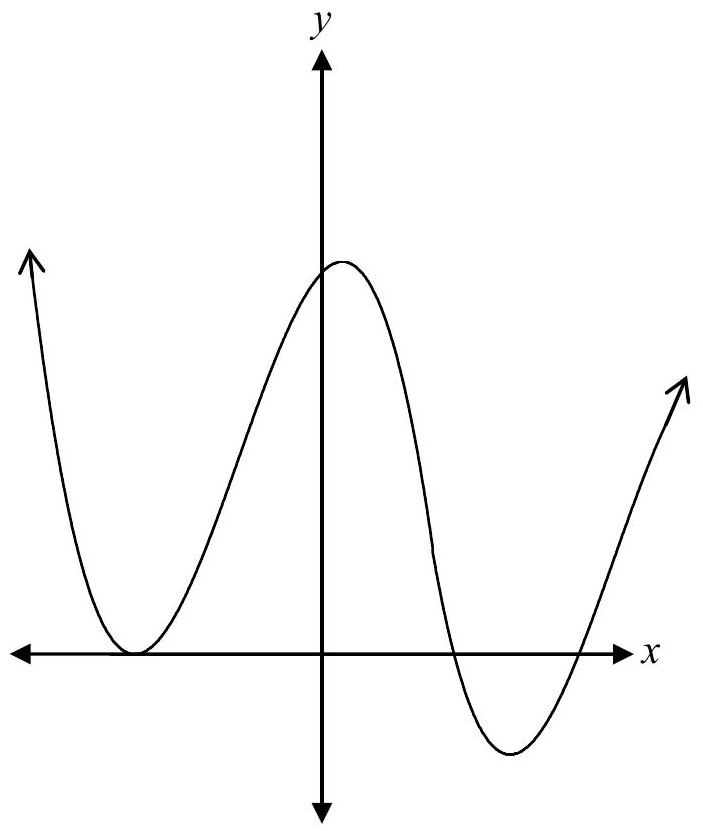
\includegraphics[max width=\textwidth, alt={}, center]{de5fb11a-28c7-4ac7-b7ff-0309cebac724-151_831_703_429_1142}

When the point $(-4,-3)$ is reflected in the line $y=x$, the coordinates of the new point are:\\
a) (-3, -4)\\
b) $(3,4)$\\
c) $(4,-3)$\\
d) $(-4,3)$\\
a) Sketch the graph of $y=\left(\frac{1}{4}\right)^{x}$.\\
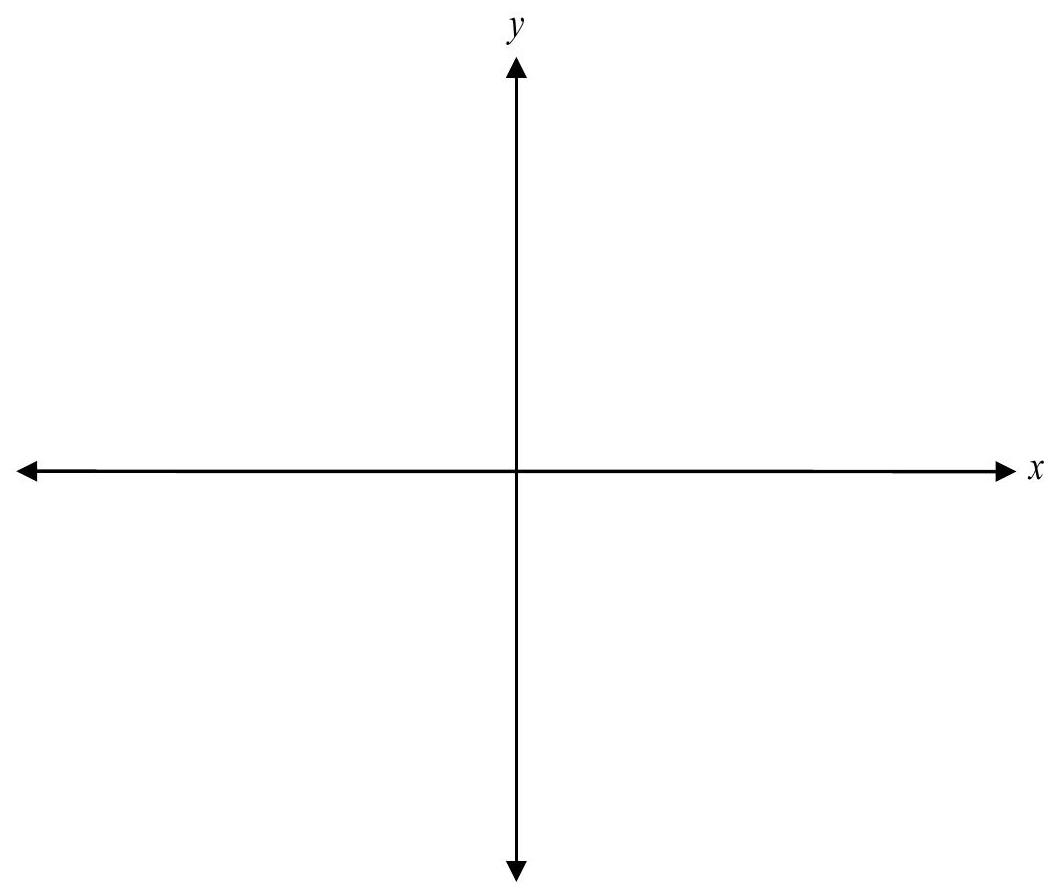
\includegraphics[max width=\textwidth, alt={}, center]{de5fb11a-28c7-4ac7-b7ff-0309cebac724-152_894_1056_509_468}\\
b) Sketch the graph of $y=2\left(\frac{1}{4}\right)^{x}$.\\
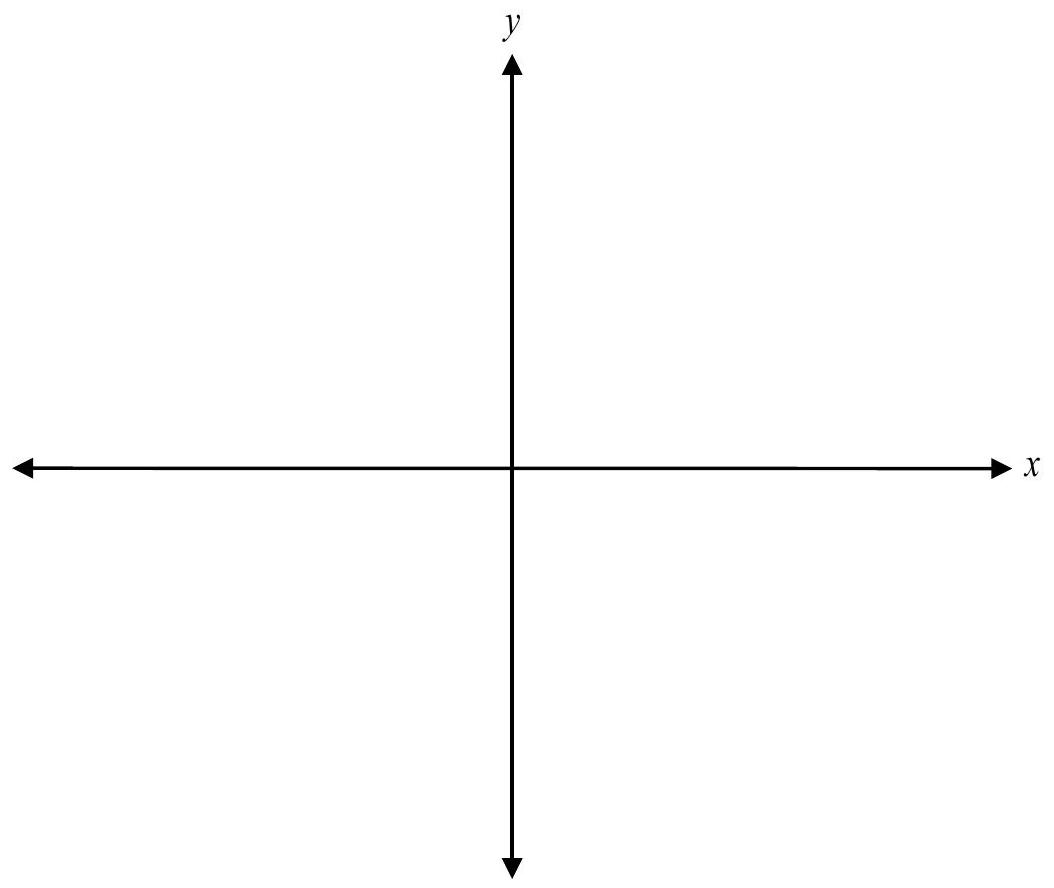
\includegraphics[max width=\textwidth, alt={}, center]{de5fb11a-28c7-4ac7-b7ff-0309cebac724-152_888_1054_1583_468}

Determine all of the zeroes of the function $p(x)=x^{3}-5 x^{2}-2 x+24$, given one of the factors of $p(x)$ is $(x-3)$.

Given the graph of $f(x)$,\\
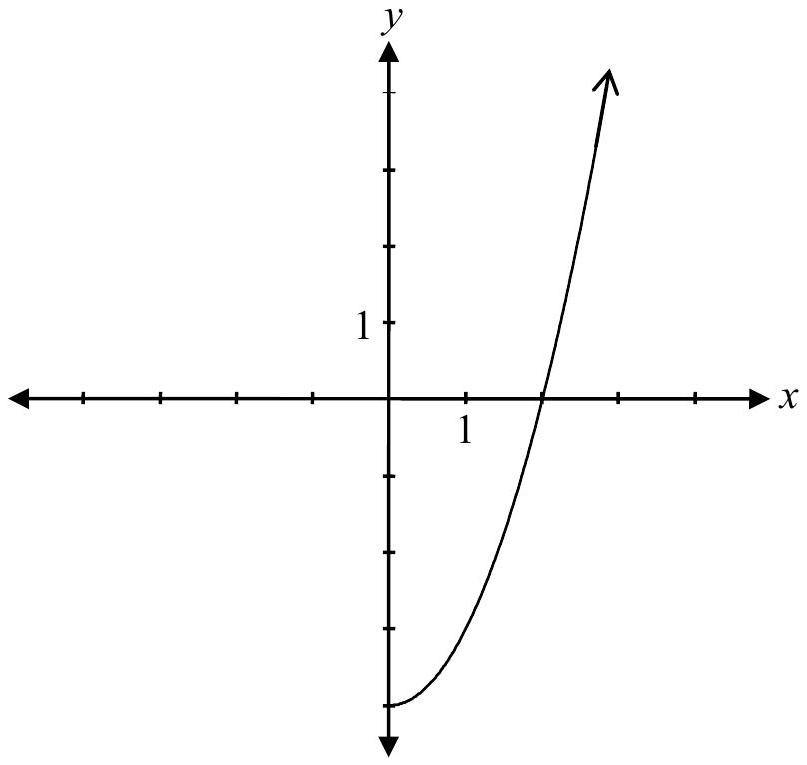
\includegraphics[max width=\textwidth, alt={}, center]{de5fb11a-28c7-4ac7-b7ff-0309cebac724-154_765_807_464_257}\\
sketch the graph of $y=\sqrt{f(x)}$.\\
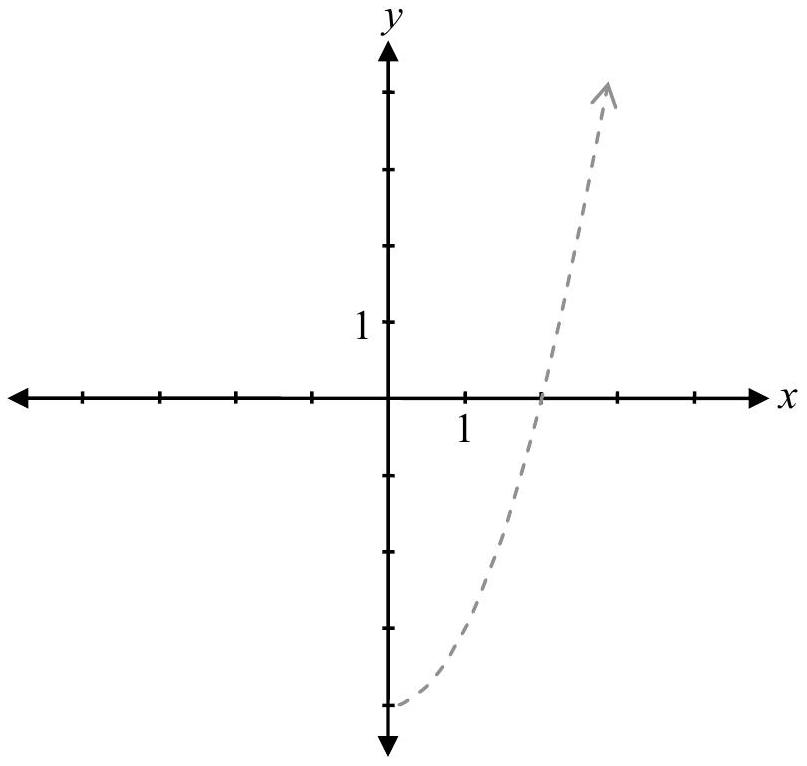
\includegraphics[max width=\textwidth, alt={}, center]{de5fb11a-28c7-4ac7-b7ff-0309cebac724-154_766_807_1602_562}

The graph of $f(x)$ has already been drawn for your reference.

No marks will be awarded for the graph of $f(x)$.

Sketch the graph of at least one period of the function $y=-2 \sin (4 x)$.\\
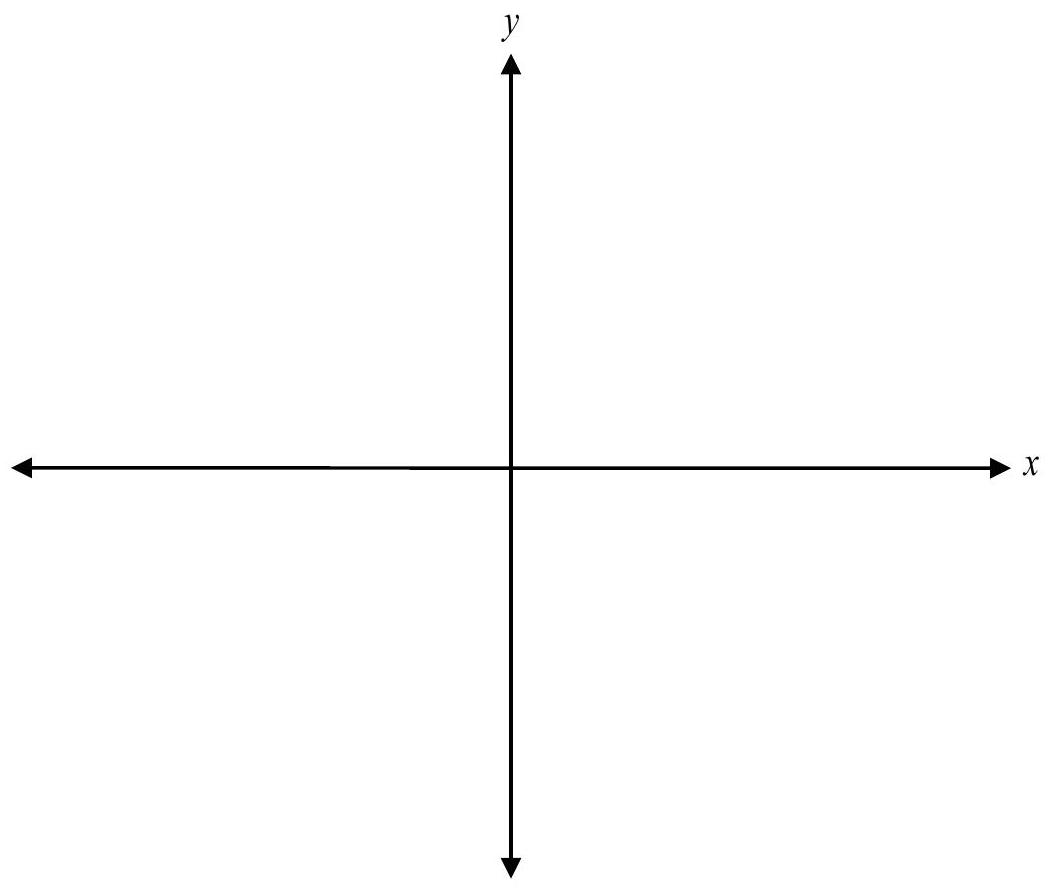
\includegraphics[max width=\textwidth, alt={}, center]{de5fb11a-28c7-4ac7-b7ff-0309cebac724-155_888_1056_554_515}

Evaluate:

$$
\frac{1}{2} \log _{3} 144-\log _{3} 4+2 \log _{3} 3
$$

Match each function with its correct description.\\
a) The graph of this function has a vertical asymptote at $x=-1$.\\
b) The graph of this function has a point of discontinuity (hole) at $x=3$.\\
c) The graph of this function has a horizontal asymptote at $y=4$.\\
d) The domain of this function is $x \in \mathbb{R}$.

Place the appropriate letter in this column.\\
$f(x)=\frac{4}{x^{2}+1}$\\
$g(x)=\frac{4 x}{x+3}$\\
$h(x)=\frac{4(x-3)(x+2)}{(x-3)}$\\
$k(x)=\frac{4(x-3)}{(x+3)(x+1)}$

The point $(-3,4)$ is on the graph of $y=\frac{1}{2} f(3 x)$.\\
State the coordinates of the corresponding point on the graph of $y=f(x)$.

Sketch the graph of $y=-2(x-1)(x-3)(x+1)$.\\
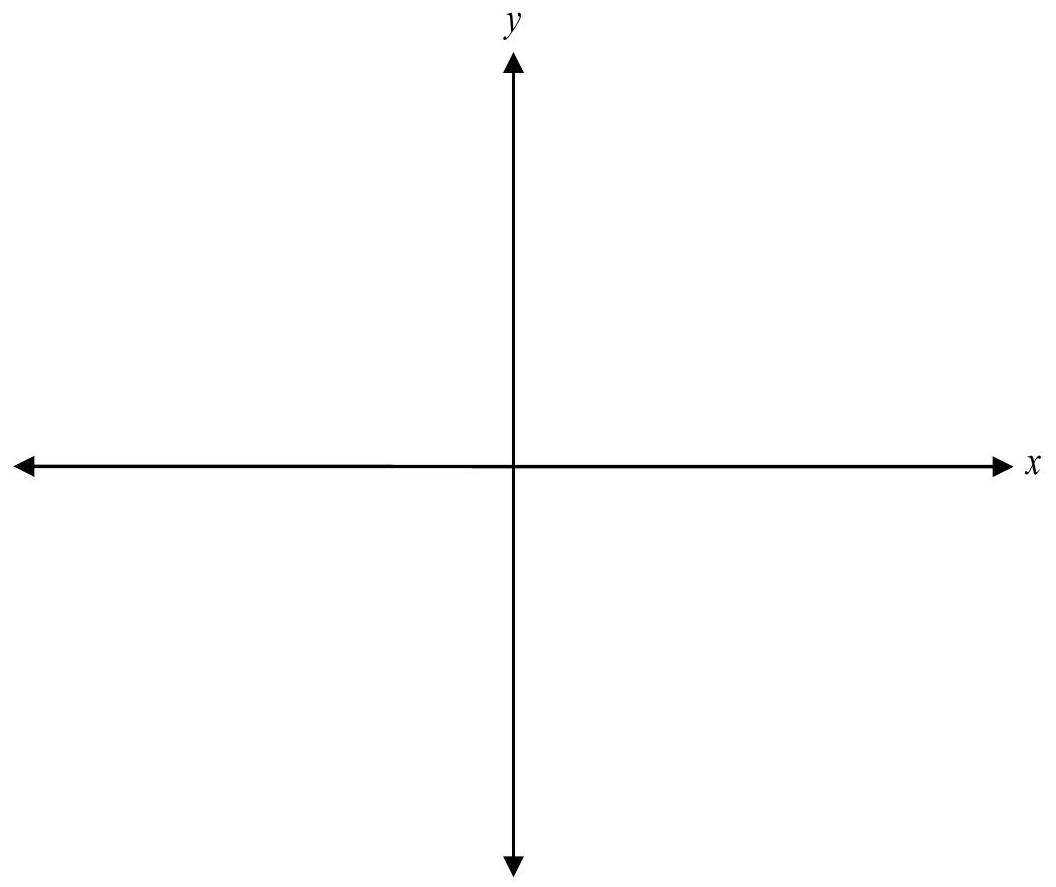
\includegraphics[max width=\textwidth, alt={}, center]{de5fb11a-28c7-4ac7-b7ff-0309cebac724-159_887_1056_605_515}\\
a) Verify that the equation $\frac{1-\sin ^{2} x}{\cos x}=\frac{\sin 2 x}{2 \sin x}$ is true for $x=\frac{\pi}{3}$.

\begin{center}
\begin{tabular}{|l|l|}
\hline
Left-Hand Side & Right-Hand Side \\
\hline
 &  \\
\hline
\end{tabular}
\end{center}

b) Explain why verifying the equation for $x=\frac{\pi}{3}$ is insufficient to conclude that the equation is an identity.

Evaluate:

$$
\frac{{ }_{7} P_{2}}{{ }_{7} P_{5}}
$$

Use the graph of $y=f(x)$ to sketch the graph of $y=f(3 x)+1$.\\
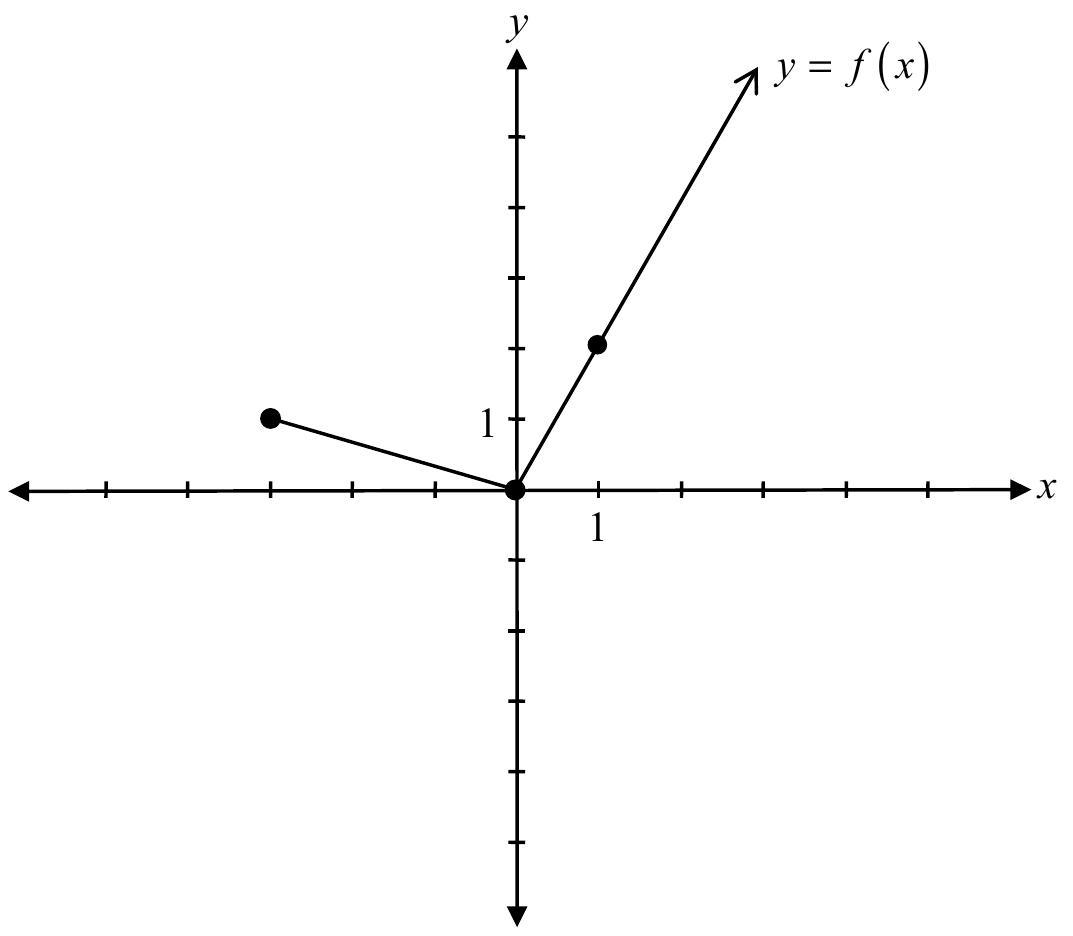
\includegraphics[max width=\textwidth, alt={}, center]{de5fb11a-28c7-4ac7-b7ff-0309cebac724-162_936_1073_472_464}\\
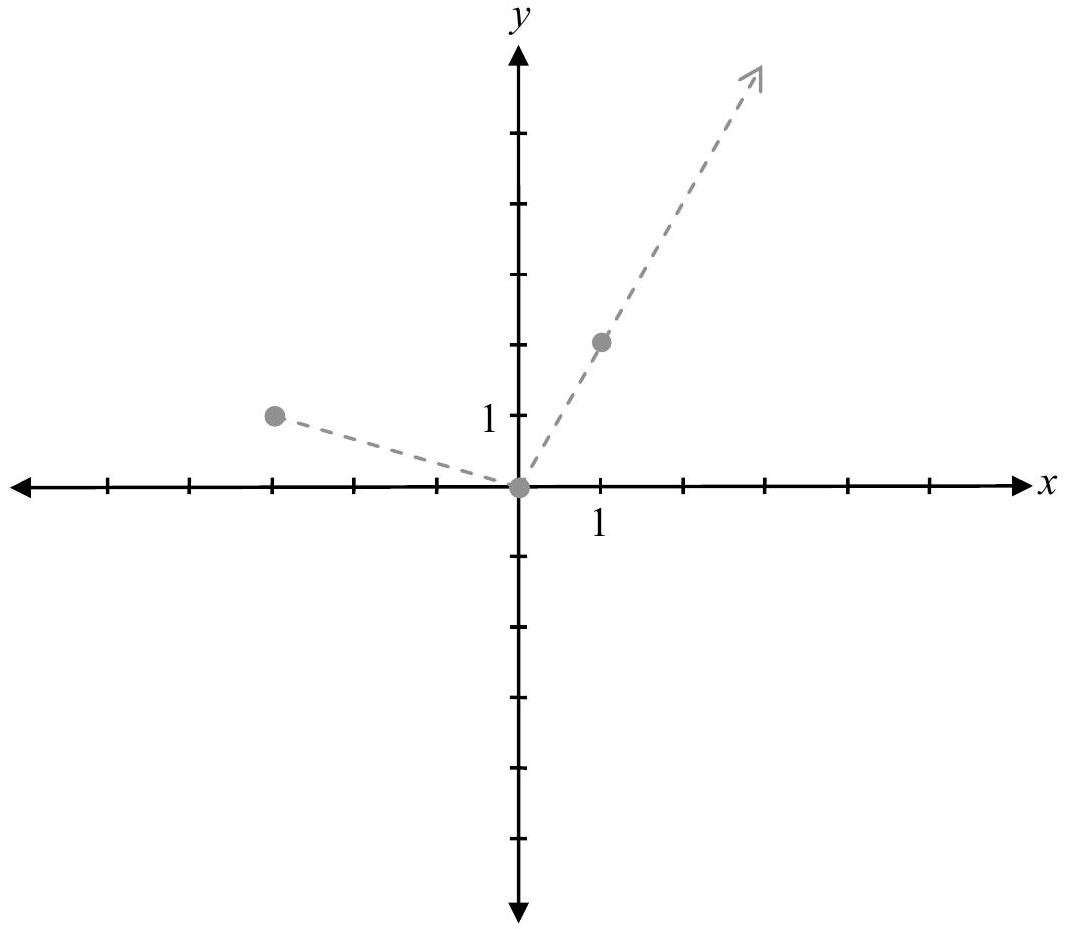
\includegraphics[max width=\textwidth, alt={}, center]{de5fb11a-28c7-4ac7-b7ff-0309cebac724-162_929_1069_1583_302}

The graph of $f(x)$ has already been drawn for your reference.

No marks will be awarded for the graph of $f(x)$.

Solve the following equation:

$$
\log _{4}(x+2)+\log _{4} 3=\log _{4} x
$$

Determine the coordinates of the point of discontinuity (hole) for the graph of the function $y=\frac{(2-x)(x-3)}{(x-2)}$.

Evaluate and simplify $\sec \left(\frac{5 \pi}{6}\right) \cdot \tan \left(-\frac{\pi}{6}\right)$.

Sketch the graph of the following function:

$$
y=-2 \sqrt{x-3}
$$

\begin{center}
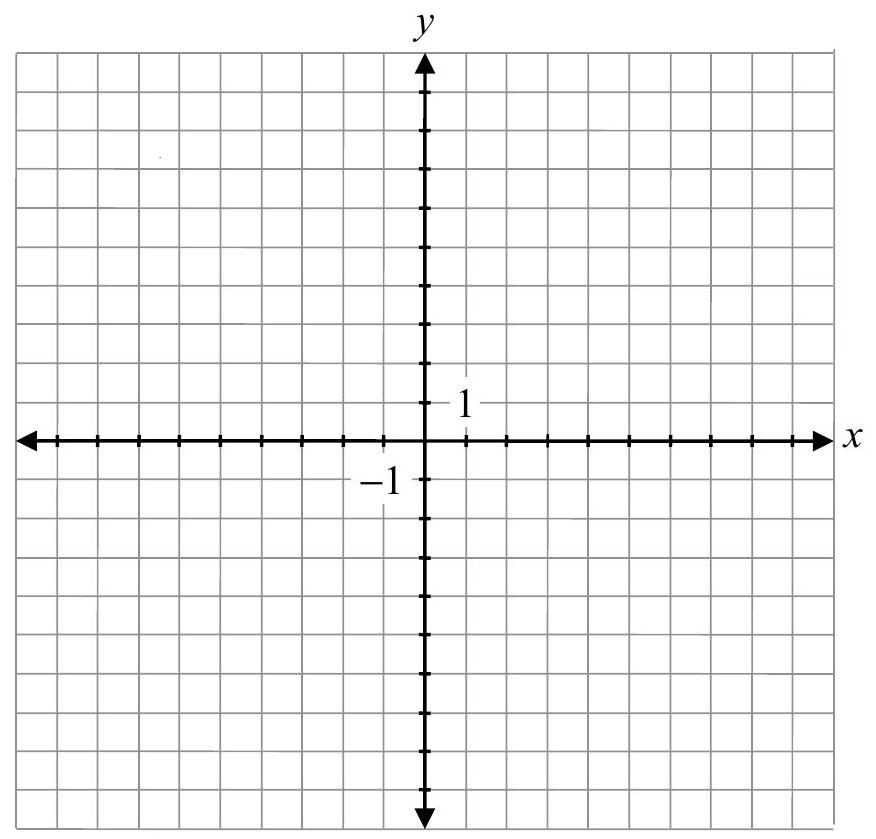
\includegraphics[max width=\textwidth, alt={}]{de5fb11a-28c7-4ac7-b7ff-0309cebac724-166_839_876_586_575}
\end{center}

Sketch the graph of $f(x)=\frac{2 x+3}{x+2}$.\\
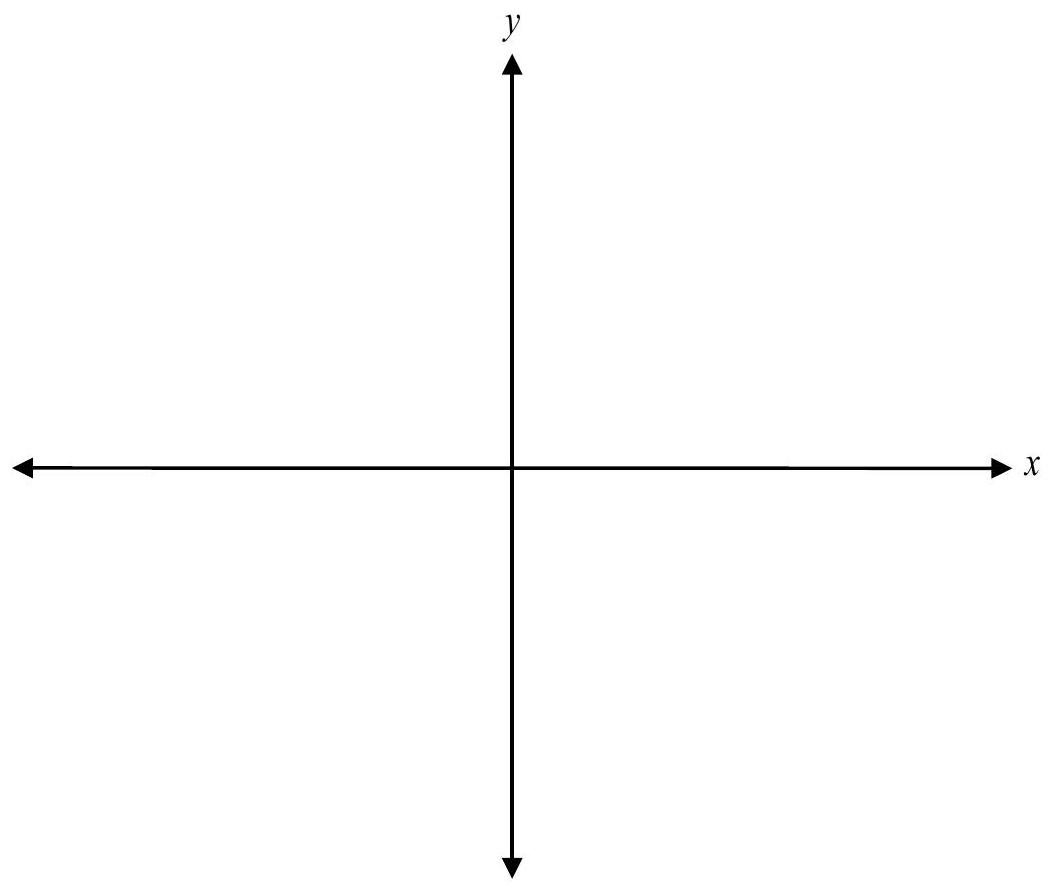
\includegraphics[max width=\textwidth, alt={}, center]{de5fb11a-28c7-4ac7-b7ff-0309cebac724-167_888_1052_627_558}

\section*{Question 42}
a) 2 marks\\
b) 1 mark138\\
139\\
a) Given the functions $f(x)=\sqrt{4+x}$ and $g(x)=|3 x-6|$, evaluate $f(g(-5))$.\\
b) Is it possible to evaluate $g(f(-5))$ ?

Justify your answer.

Identify which of these values is greater. Justify your answer.

$$
\log _{5} 80 \text { or } \log _{3} 30
$$

Given $\cos \alpha=\frac{3}{5}$, where $\alpha$ is in quadrant IV, and $\cos \beta=-\frac{2}{3}$, where $\beta$ is in quadrant II, determine the exact value of $\sin (\alpha-\beta)$.

Determine the number of possible sandwiches from the following menu.

\begin{center}
\begin{tabular}{cccc}
\multicolumn{4}{c}{MENU} \\
\hline
\multicolumn{4}{c}{Select one item from each column:} \\
\begin{tabular}{c}
Bread \\
White \\
\end{tabular} & \begin{tabular}{l}
Sauce \\
Rye \\
Brown \\
\end{tabular} & \begin{tabular}{c}
Mayo \\
Mustard \\
\end{tabular} & \begin{tabular}{c}
Turkey \\
Ham \\
Roast Beef \\
Chicken \\
\end{tabular} \\
\end{tabular}
\end{center} \begin{tabular}{c}
Vegetable \\
Tomato \\
Onion \\
Lettuce \\
\end{tabular}

Use the information in the diagram to determine the value of the arc length " $s$ ", given the central angle of $56^{\circ}$.\\
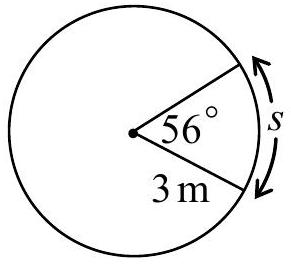
\includegraphics[max width=\textwidth, alt={}, center]{de5fb11a-28c7-4ac7-b7ff-0309cebac724-172_265_291_502_573}

Solve $\tan ^{2} \theta-5 \tan \theta+4=0$ where $\theta \in \mathbb{R}$.

Solve:

$$
2^{5 x}=3(5)^{x-3}
$$

David and Sarah are in a class of 10 boys and 8 girls.\\
A committee of 3 boys and 2 girls is to be selected from the students in this class.\\
Determine the number of possible committees if David and Sarah cannot be on the same committee.

In the binomial expansion of $\left(\frac{3}{x^{2}}-x^{5}\right)^{10}$, simplify the 7 th term.

A lake affected by acid rain has a pH of 4.4.\\
A person suffering from heartburn has a stomach acid pH of 1.2.\\
The pH of a solution is defined as $\mathrm{pH}=-\log \left[\mathrm{H}^{+}\right]$where $\left[\mathrm{H}^{+}\right]$is the hydrogen ion concentration.\\
How many times greater is the hydrogen ion concentration of the stomach than that of the lake?\\
Express your answer as a whole number.

Solve the following equation algebraically over the interval $[0,2 \pi]$.

$$
\cos 2 \theta-3 \sin \theta-2=0
$$

Explain how the value of $n$ affects the behaviour of the graph of the polynomial function $p(x)=(x+3)(x-1)^{n}$, as $p(x)$ approaches the $x$-intercept at $x=1$.

Sketch the angle $-320^{\circ}$ in standard position.\\
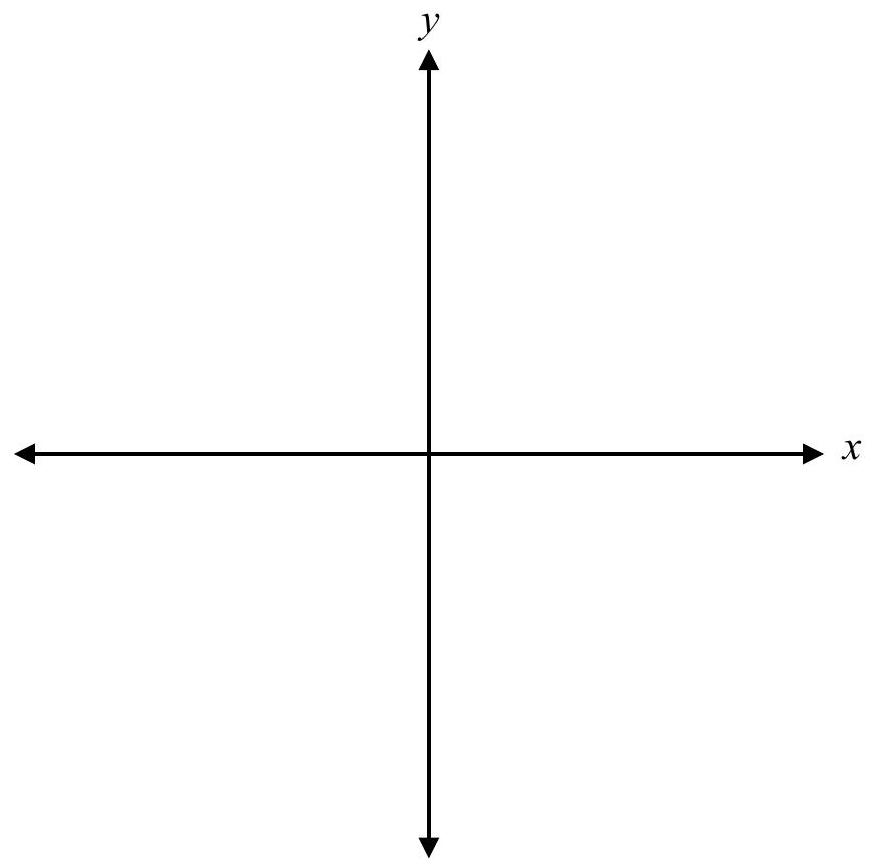
\includegraphics[max width=\textwidth, alt={}, center]{de5fb11a-28c7-4ac7-b7ff-0309cebac724-180_866_873_494_526}

Given the graph of $y=f(x)$, explain how to graph $y=f(-x)$.\\
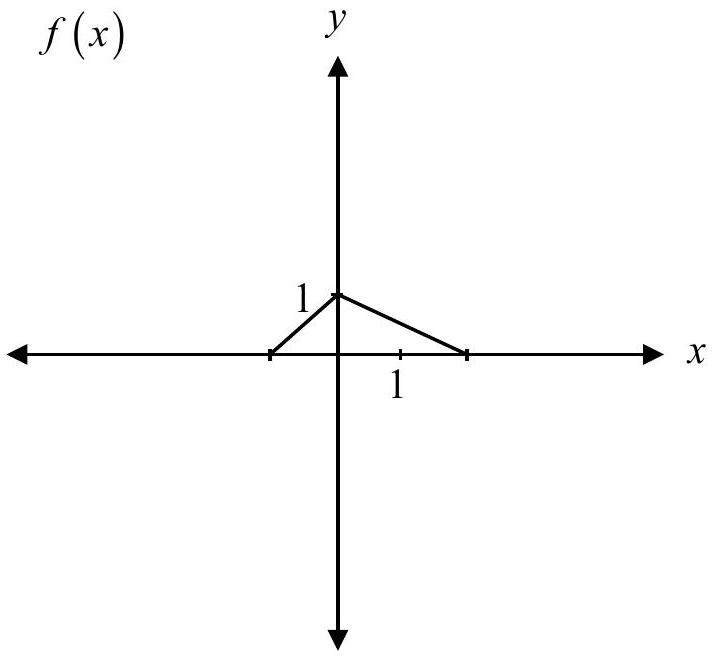
\includegraphics[max width=\textwidth, alt={}, center]{de5fb11a-28c7-4ac7-b7ff-0309cebac724-181_656_714_545_348}

Explain how the graph of $y=\frac{3(x-1)}{(x-1)}$ is different than the graph of $y=3$.

Given the graph of $f(x)$, sketch the graph of $g(x)=2 f(3 x)$.\\
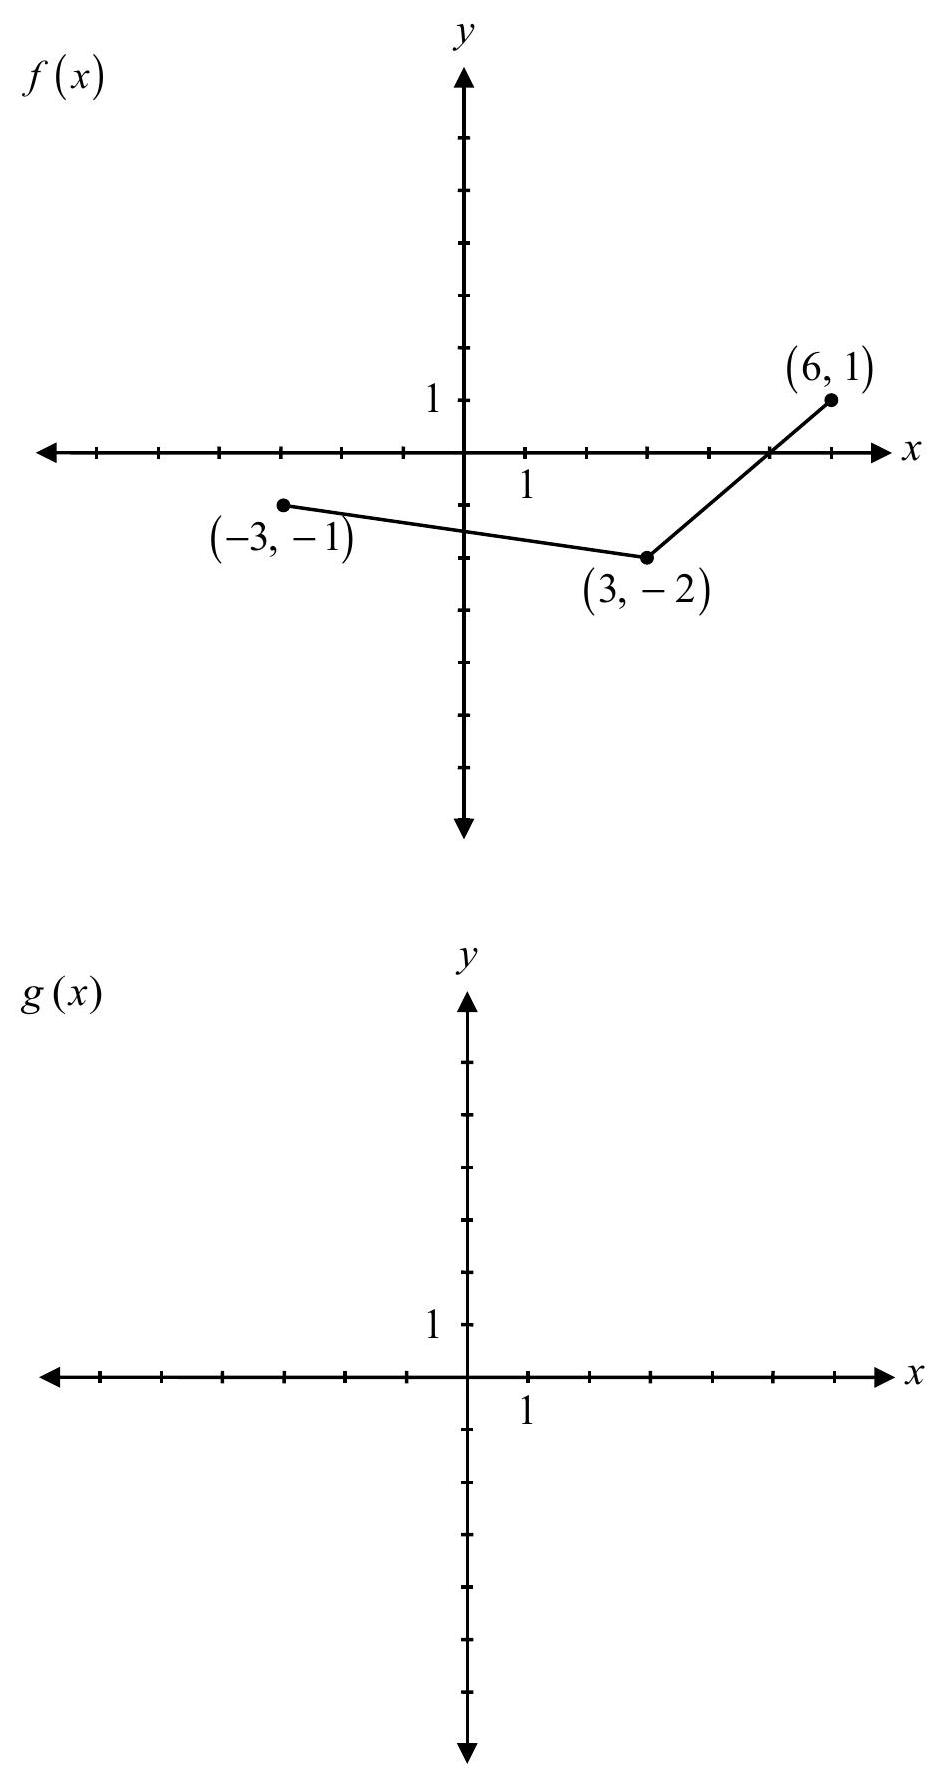
\includegraphics[max width=\textwidth, alt={}, center]{de5fb11a-28c7-4ac7-b7ff-0309cebac724-183_1778_942_487_457}

Determine the equation of the radical function represented by the graph.\\
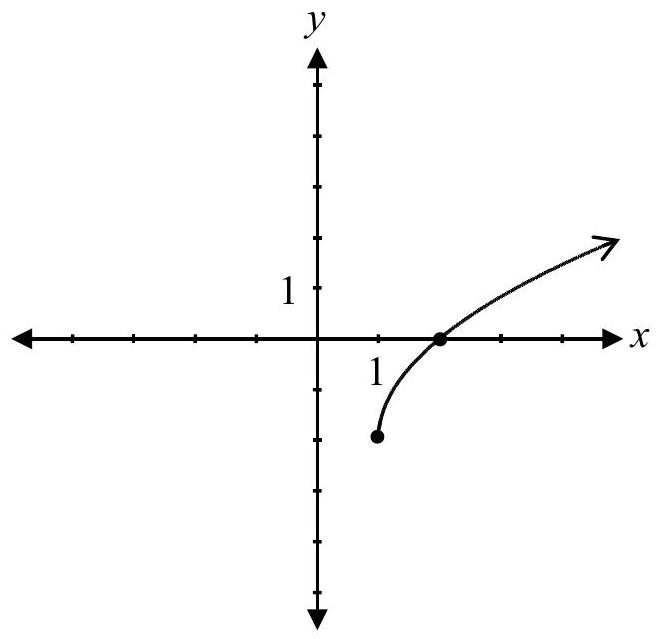
\includegraphics[max width=\textwidth, alt={}, center]{de5fb11a-28c7-4ac7-b7ff-0309cebac724-184_639_660_524_425}

There are 2 types of pencils, 3 colours of highlighters, and 5 styles of pens.\\
If you must select one of each to form a set, how many different sets of writing instruments are possible?\\
a) 10\\
b) 11\\
c) 25\\
d) 30

The point $P(\theta)$ lies on the unit circle. What are the coordinates of the point $P$ if $\theta=120^{\circ}$ ?\\
a) $\left(-\frac{1}{2}, \frac{\sqrt{3}}{2}\right)$\\
b) $\left(-\frac{\sqrt{3}}{2},-\frac{1}{2}\right)$\\
c) $\left(-\frac{\sqrt{3}}{2}, \frac{1}{2}\right)$\\
d) $\left(\frac{1}{2}, \frac{\sqrt{3}}{2}\right)$

Identify the function that has a domain of $\{x \mid x \geq 7\}$ and a range of $\{y \mid y \geq 0\}$.\\
a) $f(x)=\sqrt{x}+7$\\
b) $f(x)=\sqrt{x}-7$\\
c) $f(x)=\sqrt{x+7}$\\
d) $f(x)=\sqrt{x-7}$

\section*{Question 17}
Using $y=-10 \cos [\mathrm{~B}(x-\mathrm{C})]+\mathrm{D}$, the value of C that corresponds to the following graph is:\\
a) 5\\
b) 10\\
c) 15\\
d) 20\\
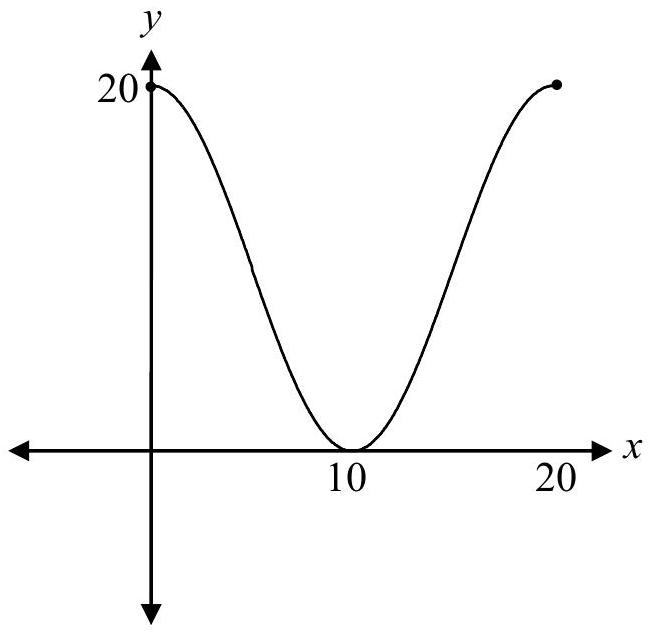
\includegraphics[max width=\textwidth, alt={}, center]{de5fb11a-28c7-4ac7-b7ff-0309cebac724-186_635_654_1585_782}

Given the following row of Pascal's Triangle, identify the binomial expansion with these coefficients.\\
$\begin{array}{llllll}1 & 5 & 10 & 10 & 5 & 1\end{array}$\\
a) $(x+y)^{4}$\\
b) $(x+y)^{5}$\\
c) $(x+y)^{6}$\\
d) $(x+y)^{7}$

Question 19

Identify the graph of the function $f(x)=-(x-2)(x-1)^{2}(x+1)$.\\
a)\\
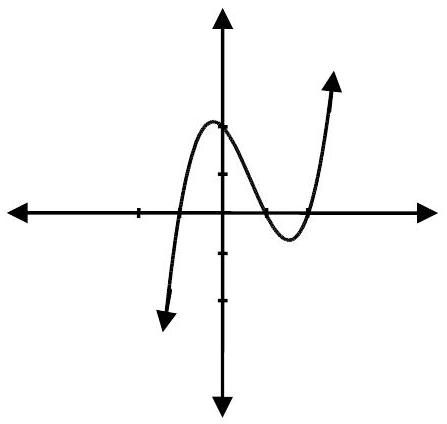
\includegraphics[max width=\textwidth, alt={}, center]{de5fb11a-28c7-4ac7-b7ff-0309cebac724-187_424_447_1497_348}\\
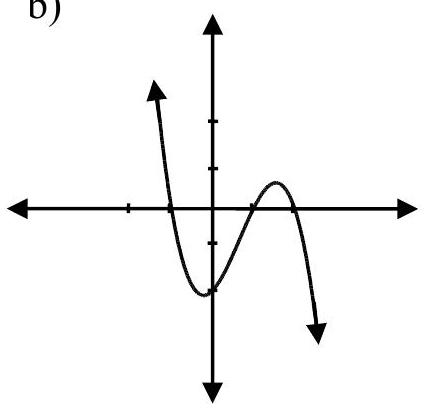
\includegraphics[max width=\textwidth, alt={}, center]{de5fb11a-28c7-4ac7-b7ff-0309cebac724-187_413_424_1508_1035}\\
c)\\
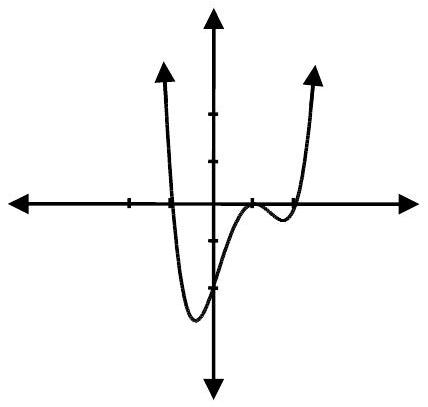
\includegraphics[max width=\textwidth, alt={}, center]{de5fb11a-28c7-4ac7-b7ff-0309cebac724-187_407_428_2015_352}\\
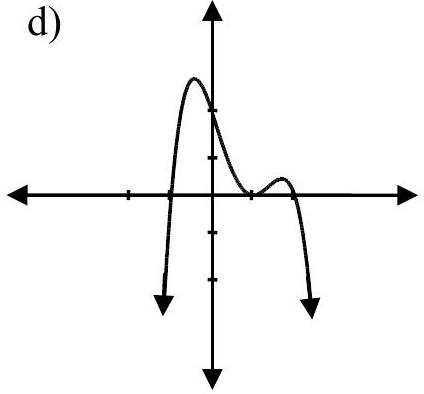
\includegraphics[max width=\textwidth, alt={}, center]{de5fb11a-28c7-4ac7-b7ff-0309cebac724-187_394_424_2028_1035}

Determine the value of $\log _{9}\left(\log _{3} 27\right)$.\\
a) $\frac{1}{3}$\\
b) $\frac{1}{2}$\\
c) 2\\
d) 3

If $(x, y)$ is a point on the graph of $y=f(x)$, identify the coordinates of this point on the graph of $g(x)=f(2 x)+5$.\\
a) $\left(\frac{x}{2}, y+5\right)$\\
b) $(2 x, y+5)$\\
c) $\left(\frac{x}{2}, y-5\right)$\\
d) $\left(\frac{x}{2}-5, y\right)$

Identify an equivalent expression for $1+\log _{2} 5$.\\
a) $\log _{2} 5$\\
b) $\log _{2} 7$\\
c) $\log _{2} 10$\\
d) $\log _{2} 11$

Solve:

$$
2 \log _{4} x-\log _{4}(x+3)=1
$$

The following transformations are applied to $f(x)$, resulting in a new function, $g(x)$.

\begin{itemize}
  \item reflection over the $y$-axis
  \item horizontal translation of 3 units to the right
  \item vertical translation of 4 units down
\end{itemize}

Write the equation of $g(x)$ in terms of $f(x)$.

$$
g(x)=
$$

\section*{Question 25}
a) 3 marks\\
b) 1 mark116\\
117

The height of a bicycle pedal as the bicycle is moving at a constant speed can be represented by the following function:

$$
h(t)=15 \cos \frac{2 \pi}{5} t+30
$$

where $h$ is the height of the pedal above the ground, in cm , and $t$ is the time, in seconds.\\
a) Sketch a graph of at least one period of this function, where $t \geq 0$.\\
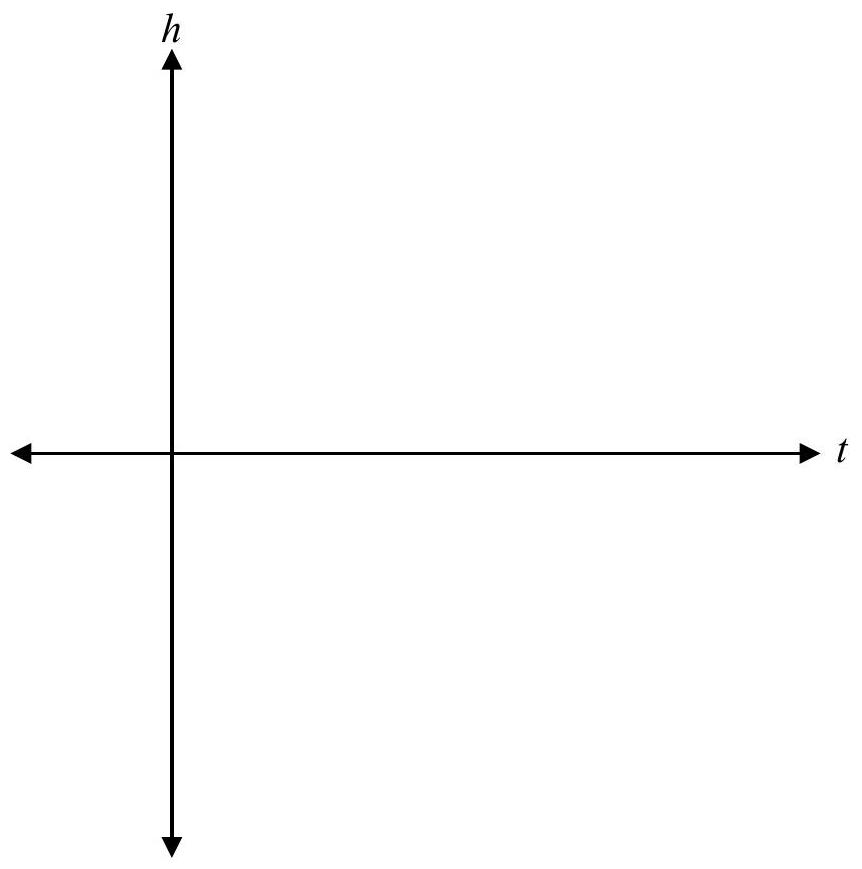
\includegraphics[max width=\textwidth, alt={}, center]{de5fb11a-28c7-4ac7-b7ff-0309cebac724-192_869_862_803_638}\\
b) Determine the height of the bicycle pedal at 7.5 seconds.

Sketch the graph of the function $f(x)$ and determine the $y$-intercept.

$$
f(x)=\frac{4}{(x-2)(x+2)}
$$

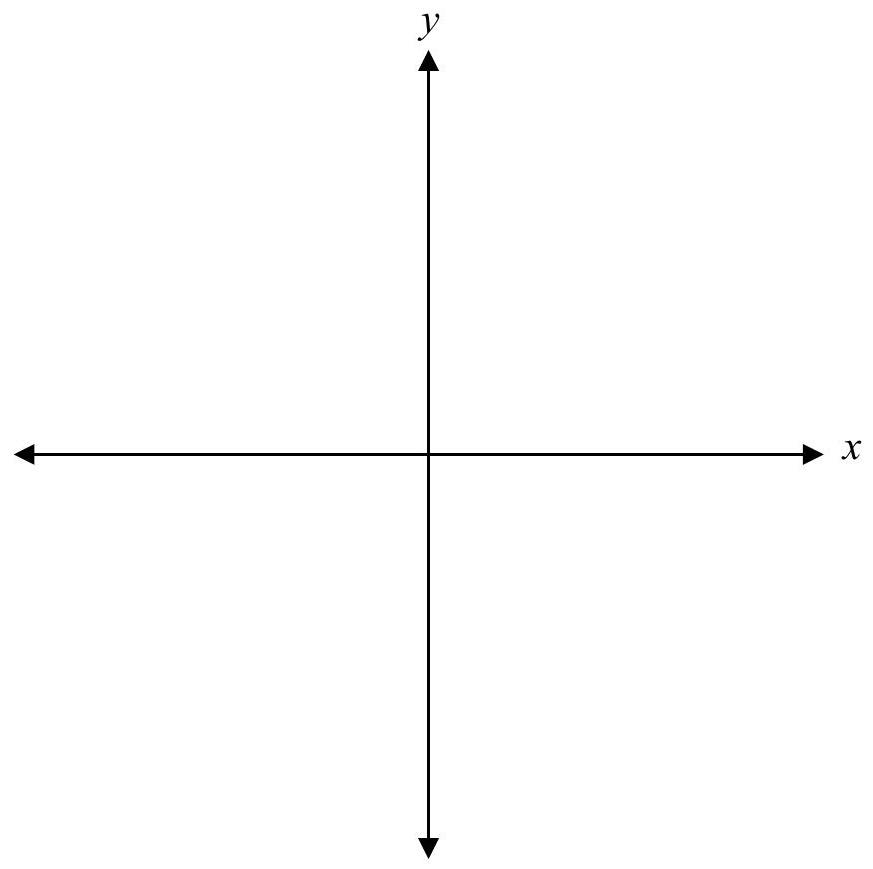
\includegraphics[max width=\textwidth, alt={}, center]{de5fb11a-28c7-4ac7-b7ff-0309cebac724-193_869_873_640_586}\\
$y$-intercept: $\_\_\_\_$

Kim solved the following logarithmic equation:

$$
\begin{gathered}
\log _{2}\left(-\frac{x}{3}\right)=\log _{2}(x-4) \\
-\frac{x}{3}=x-4 \\
-x=3 x-12 \\
-4 x=-12 \\
x \leq 3
\end{gathered}
$$

Explain why $x=3$ is an extraneous solution.

Determine the equation of the polynomial function represented by the graph.\\
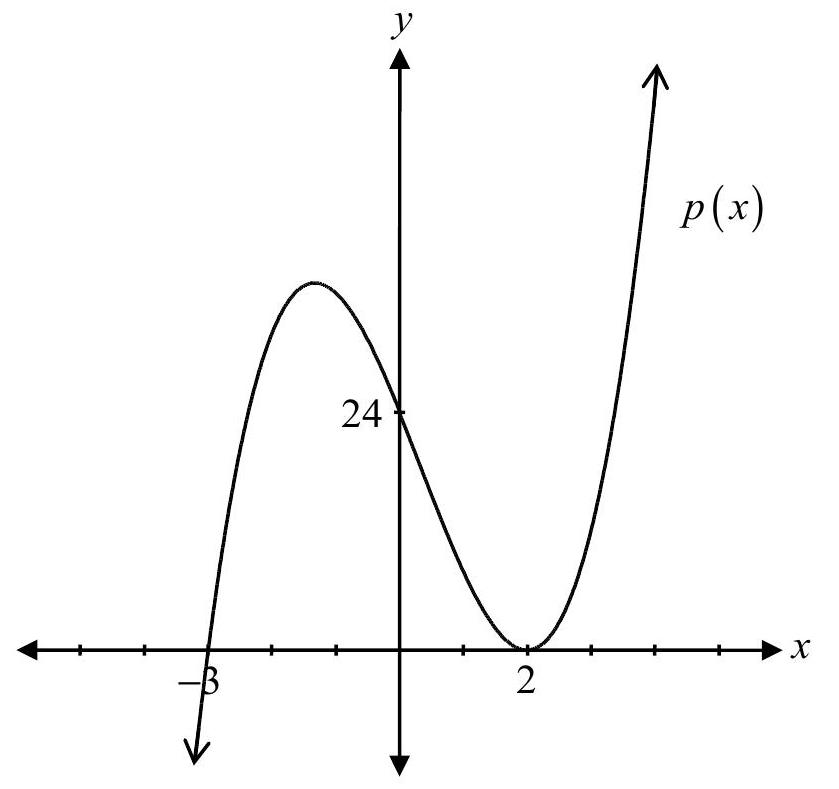
\includegraphics[max width=\textwidth, alt={}, center]{de5fb11a-28c7-4ac7-b7ff-0309cebac724-195_789_839_481_403}\\
$p(x)=$

Determine the coterminal angles with $\frac{2 \pi}{3}$ over the interval $[-2 \pi, 4 \pi]$.\\
a) Solve the following equation:

$$
0=\sqrt{4 x-8}-2
$$

b) Explain how your answer in a) is related to the graph of $y=\sqrt{4 x-8}-2$.

Determine the exact value of $\sin \frac{13 \pi}{12}$.

\section*{Question 32}
a) 2 marks\\
b) 1 mark

Given the functions $f(x)=x+2$ and $g(x)=\frac{1}{x-5}$ :\\
a) Determine the equation of the composite function $f(g(x))$ and its domain.

$$
f(g(x))=
$$

$\_\_\_\_$\\
domain: $\_\_\_\_$\\
b) Determine the $x$-intercept and $y$-intercept of $f(g(x))$.\\
$x$-intercept: $\_\_\_\_$\\
$y$-intercept: $\_\_\_\_$\\
a) Sketch the graph of $f(x)=\log _{5}(x-1)$.\\
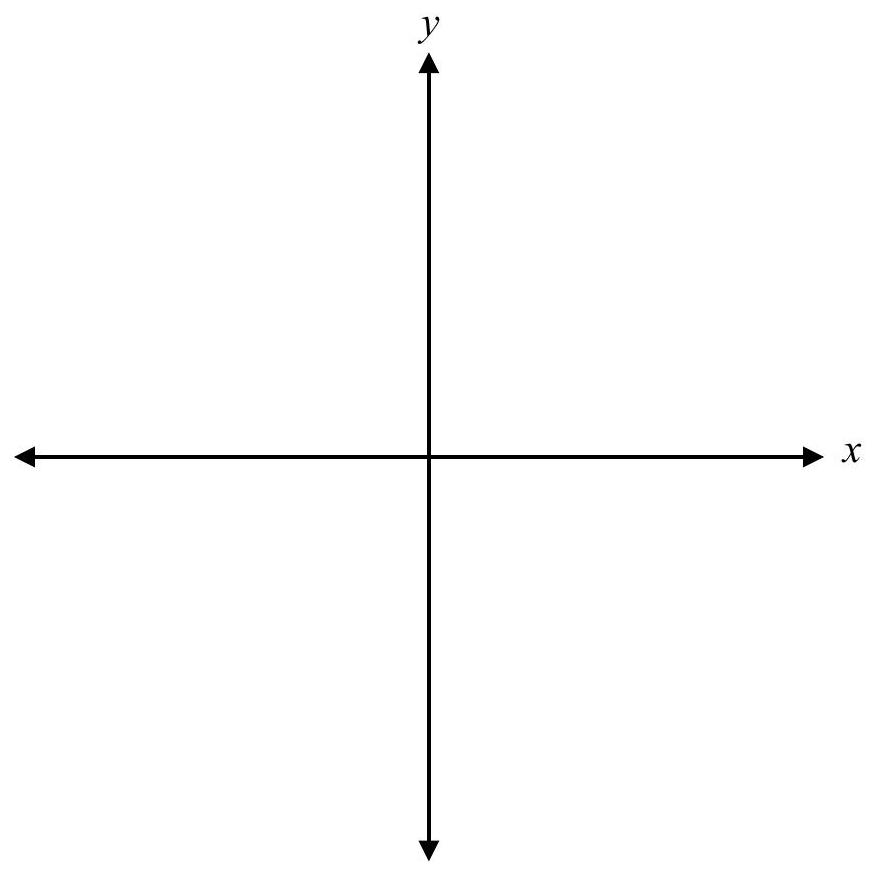
\includegraphics[max width=\textwidth, alt={}, center]{de5fb11a-28c7-4ac7-b7ff-0309cebac724-200_872_877_491_526}\\
b) Sketch the graph of $f^{-1}(x)$.\\
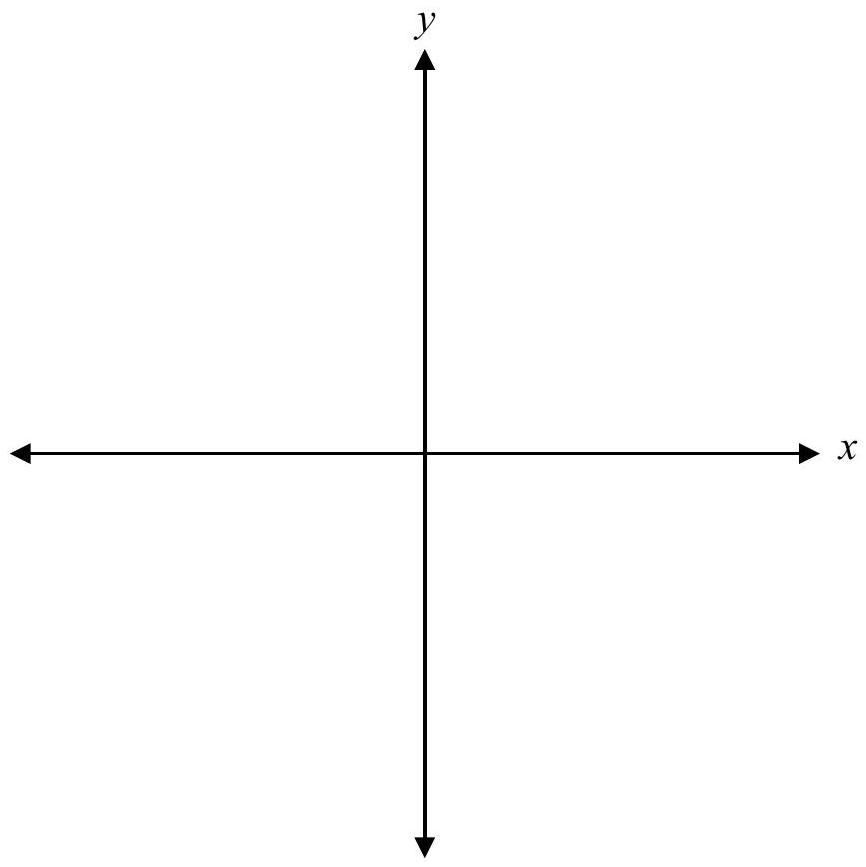
\includegraphics[max width=\textwidth, alt={}, center]{de5fb11a-28c7-4ac7-b7ff-0309cebac724-200_867_866_1570_537}

Explain what the graph of a rational function looks like near a vertical asymptote.

\section*{Question 35}
Given the graph of $f(x)=(x-2)^{2}$,\\
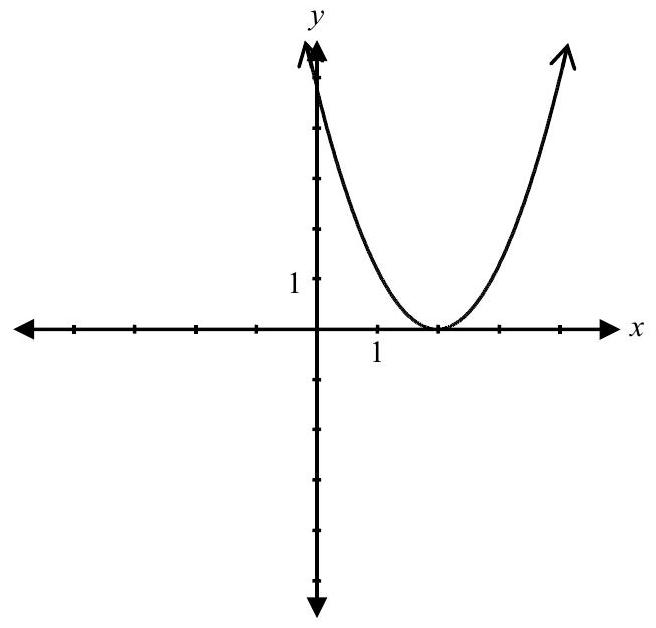
\includegraphics[max width=\textwidth, alt={}, center]{de5fb11a-28c7-4ac7-b7ff-0309cebac724-201_628_656_1465_262}\\
determine one possible restriction for the domain of $f(x)$ so that its inverse is a function.

Domain: $\_\_\_\_$

Over the interval $[0,2 \pi]$, determine the non-permissible values of $\theta$ in the expression $\csc \theta(\cos \theta+1)$.

Explain why ${ }_{3} C_{8}$ is undefined.

Solve:

$$
{ }_{n} P_{3}=48(n-1)
$$

b) 1 mark\\
c) 1 mark

Christine dives off a diving board.\\
Her dive is modelled by the function $h(t)=t^{3}-3 t^{2}-t+3$, where $h$ is her height in metres, relative to the water surface and $t$ is the time in seconds after diving off the diving board.\\
a) Given that $(t+1)$ is a factor for the function $h(t)$, determine the other factors.\\
b) Sketch the graph of the function $h(t)$ for the time interval $t=0$ to $t=3$.\\
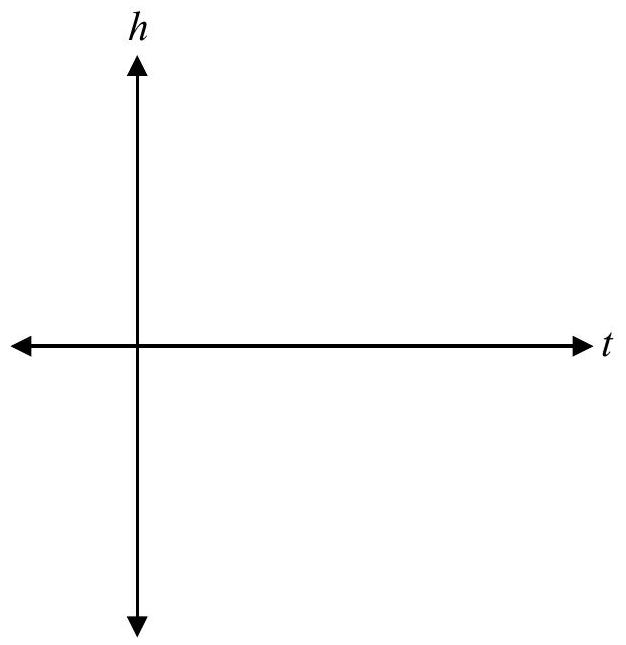
\includegraphics[max width=\textwidth, alt={}, center]{de5fb11a-28c7-4ac7-b7ff-0309cebac724-205_645_626_1450_502}\\
c) Determine how many seconds Christine is underwater.

Prove the identity for all permissible values of $x$.

$$
\sec x+\tan x=\frac{\cos x}{1-\sin x}
$$

\begin{center}
\begin{tabular}{|l|l|}
\hline
Left-Hand Side & Right-Hand Side \\
\hline
\end{tabular}
\end{center}

Given the graph of $f(x)$, sketch the graph of the function $g(x)=-|f(x)|$.\\
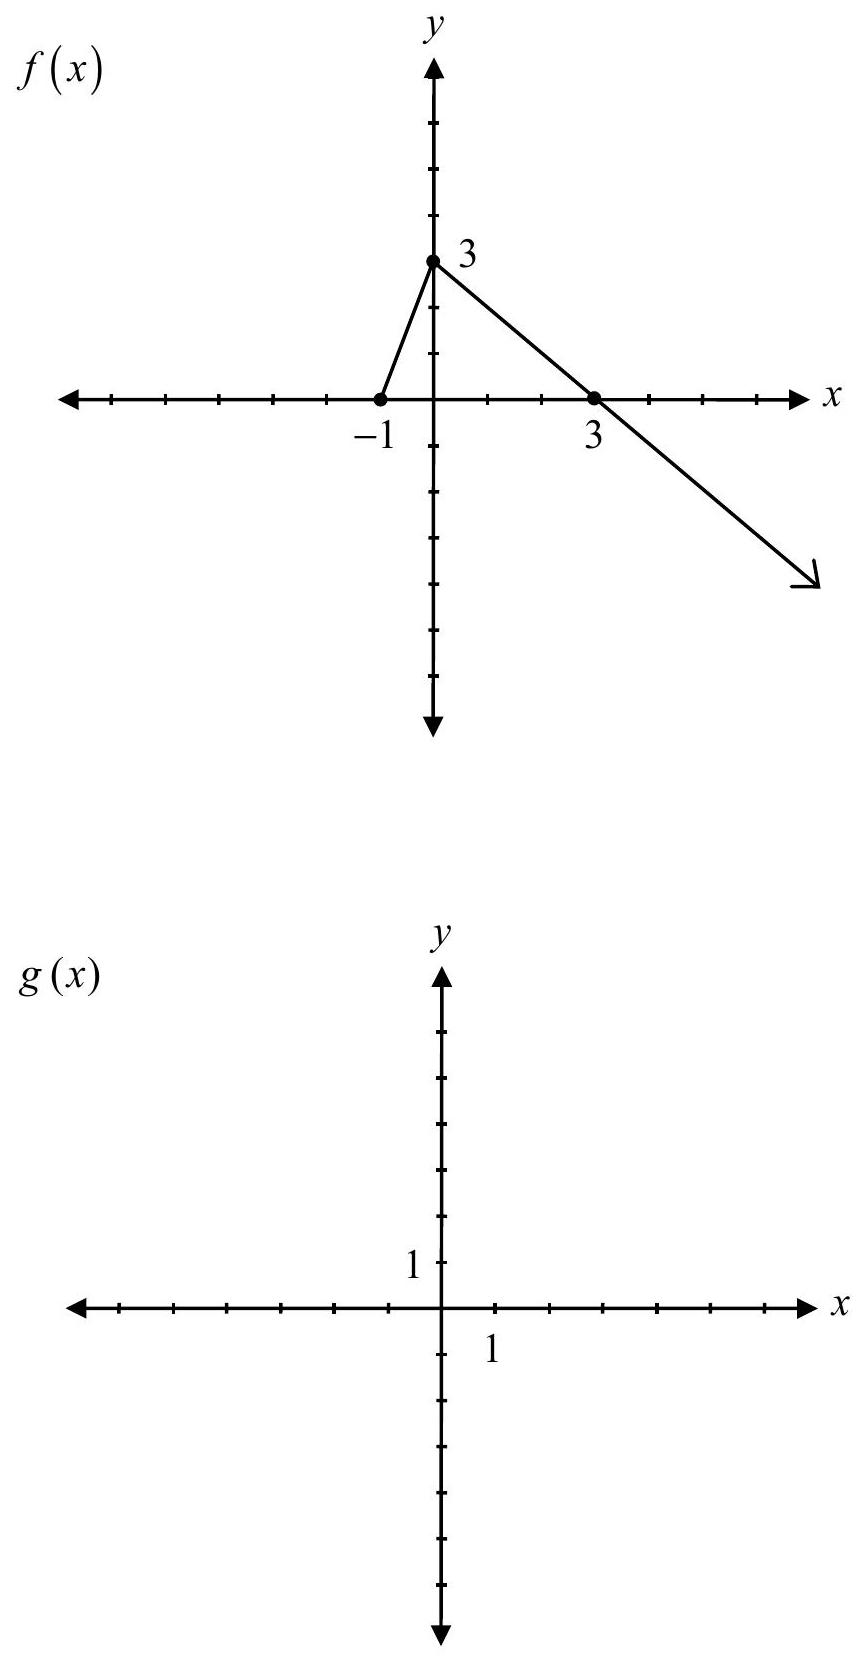
\includegraphics[max width=\textwidth, alt={}, center]{de5fb11a-28c7-4ac7-b7ff-0309cebac724-207_1658_862_499_371}

Given that $\cot \theta=-\frac{2}{5}$, where $\theta$ is in Quadrant IV, determine the exact value of $\sin \theta$.

A pizza with a diameter of 15 inches is cut into equal slices, each with a central angle of $36^{\circ}$. Determine the length of the crust on the outer edge of one slice of pizza.

There are 9 girls and 7 boys in a math class from which a committee of 5 is to be chosen.\\
a) How many different committees of 5 can be formed if one of the boys, William, must be on the committee?\\
b) How many different committees of 5 can be formed if there must be 2 girls and 3 boys on the committee?

Solve the following equation over the interval $[0,2 \pi]$ :

$$
\sin ^{2} \theta+6 \sin \theta-2=0
$$

Solve:

$$
6(5)^{3 x+2}=9^{2-x}
$$

Solve $(2 \sin \theta-1)(\sin \theta+1)=0$ where $\theta \in \mathbb{R}$.

The roots of the polynomial equation $3(x-2)(x+1)^{2}=0$ are $x=2$ and $x=-1$.\\
Explain what these roots represent on the graph of $p(x)=3(x-2)(x+1)^{2}$.

Determine an equation for $g(x)$ as a transformation of $f(x)$.\\
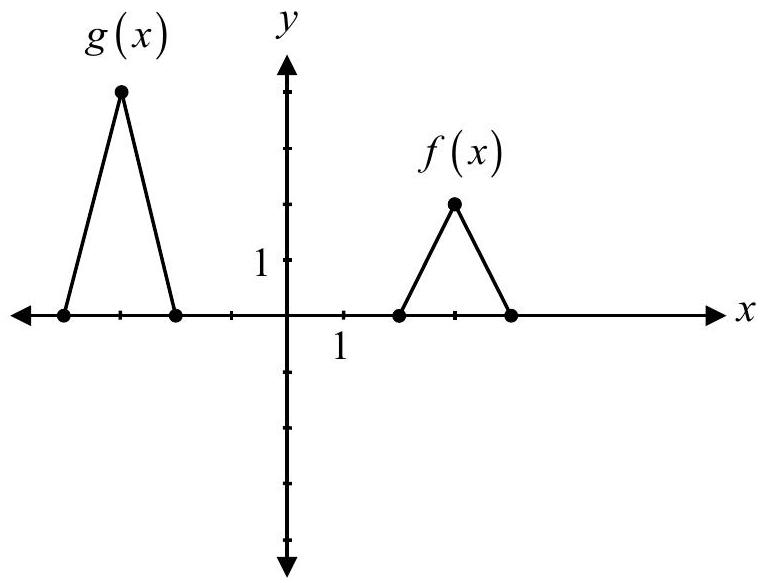
\includegraphics[max width=\textwidth, alt={}, center]{de5fb11a-28c7-4ac7-b7ff-0309cebac724-215_583_766_485_356}\\
$g(x)=$

A student must determine the factors of $5 x^{4}-2 x^{3}+4 x-1$. He used 5, $-2,4$, and -1 as the coefficients of the polynomial when using synthetic division.\\
Explain the student's error.

Describe the transformations of $y=f(x)$ when asked to sketch the graph of $y=-f(x-4)$.

Prove the identity below for all permissible values of $\theta$ :

$$
\sin \theta+\frac{\cos \theta}{\tan \theta}=\frac{1}{\cos \theta \tan \theta}
$$

\begin{center}
\begin{tabular}{|l|l|}
\hline
Left-Hand Side & Right-Hand Side \\
\hline
\end{tabular}
\end{center}

Describe how to use the graphs of $f(x)=3 \sin x$ and $g(x)=2$ to solve the equation $3 \sin x=2$.\\
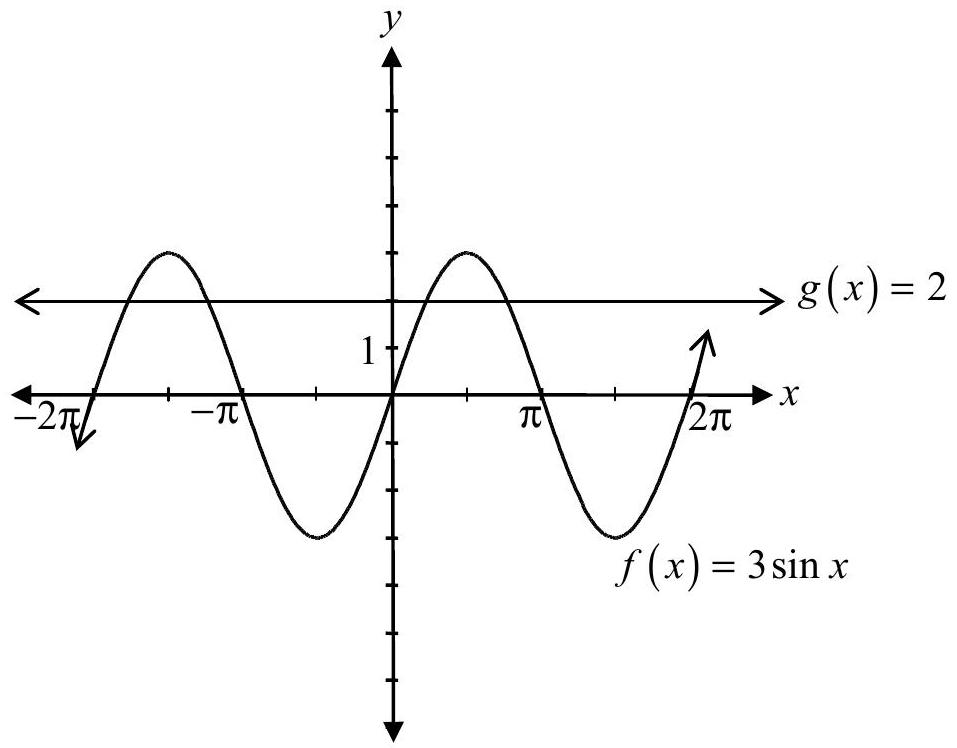
\includegraphics[max width=\textwidth, alt={}, center]{de5fb11a-28c7-4ac7-b7ff-0309cebac724-219_748_957_539_595}

A hockey arena has 5 doors.\\
Determine the number of ways that you can enter through one door but exit through a different door.

Given that $(x+3)$ is one of the factors, express $2 x^{3}+7 x^{2}+2 x-3$ as a product of factors.

Identify the maximum number of $x$-intercepts for a polynomial function of degree 3 .\\
a) 1\\
b) 2\\
c) 3\\
d) 4

\section*{Question 15}
The graph of $y=f(x)$ contains the point $(a, b)$. The graph of $g(x)$ is a transformation of the graph of $f(x)$ and contains the point ( $3 a, b$ ).

Identify the function that represents $g(x)$.\\
a) $g(x)=f(3 x)$\\
b) $g(x)=3 f(x)$\\
c) $g(x)=f\left(\frac{x}{3}\right)$\\
d) $g(x)=\frac{1}{3} f(x)$

Question 16

The angle 2.95 radians, in standard position, terminates in quadrant:\\
a) I\\
b) II\\
c) III\\
d) IV

Evaluate:

$$
2 \sin \frac{\pi}{8} \cos \frac{\pi}{8}
$$

a) $\frac{1}{2}$\\
b) $\frac{\sqrt{2}}{2}$\\
c) 1\\
d) $\sqrt{2}$

\section*{Question 18}
Identify which of the following represents the 5th term in the expansion of $\left(4 x^{2}-2 y^{3}\right)^{15}$.\\
a) ${ }_{15} C_{5}\left(4 x^{2}\right)^{10}\left(-2 y^{3}\right)^{5}$\\
b) ${ }_{15} C_{5}\left(4 x^{2}\right)^{11}\left(-2 y^{3}\right)^{4}$\\
c) ${ }_{15} C_{4}\left(4 x^{2}\right)^{10}\left(-2 y^{3}\right)^{5}$\\
d) ${ }_{15} C_{4}\left(4 x^{2}\right)^{11}\left(-2 y^{3}\right)^{4}$

Identify which of the following graphs of polynomial functions has a zero with a multiplicity of 3 .\\
a)\\
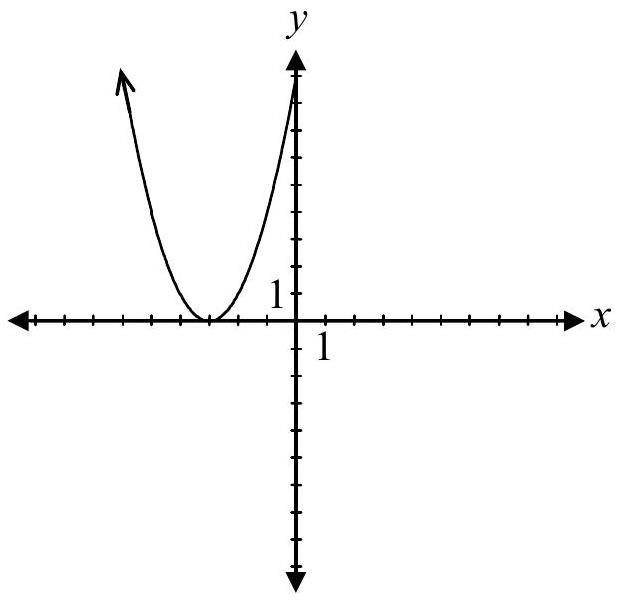
\includegraphics[max width=\textwidth, alt={}, center]{de5fb11a-28c7-4ac7-b7ff-0309cebac724-224_604_624_494_401}\\
b)\\
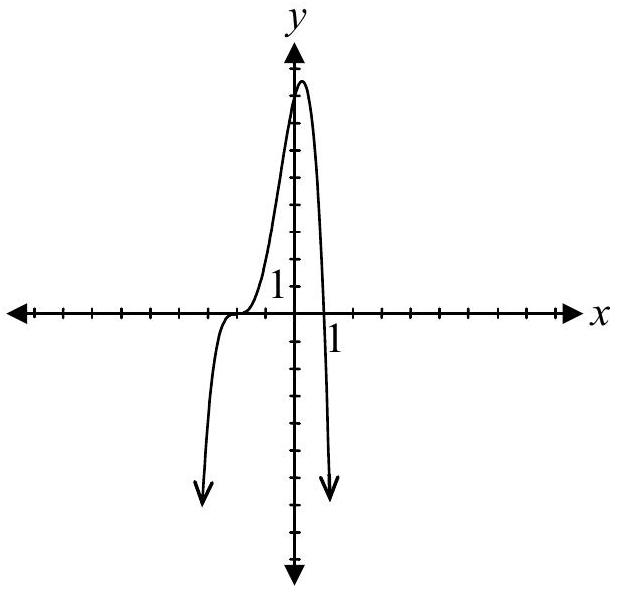
\includegraphics[max width=\textwidth, alt={}, center]{de5fb11a-28c7-4ac7-b7ff-0309cebac724-224_594_617_494_1134}\\
c)\\
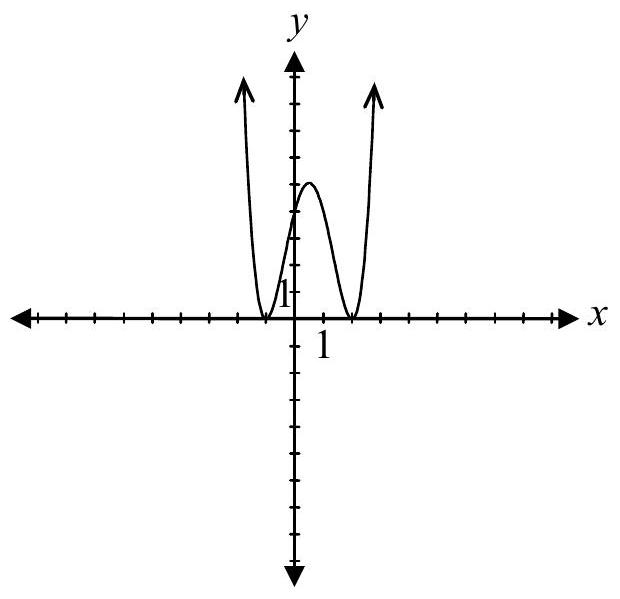
\includegraphics[max width=\textwidth, alt={}, center]{de5fb11a-28c7-4ac7-b7ff-0309cebac724-224_599_620_1213_416}\\
d)\\
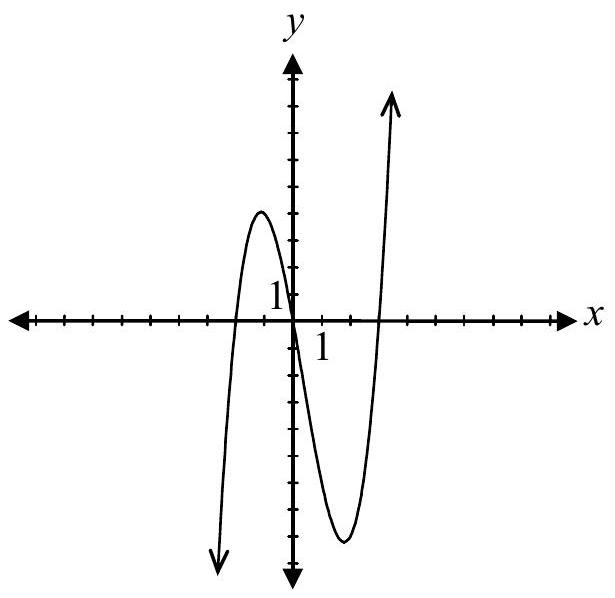
\includegraphics[max width=\textwidth, alt={}, center]{de5fb11a-28c7-4ac7-b7ff-0309cebac724-224_598_615_1211_1160}

A non-permissible value of $x$ for the function $f(x)=\frac{1}{\cos x+1}$ is:\\
a) -1\\
b) 0\\
c) $\pi$\\
d) $\frac{3 \pi}{2}$

Identify which of the following statements is true for the rational function $f(x)=\frac{4(x-1)(x-2)}{(x-1)(x+3)}$.\\
a) The equation of the horizontal asymptote is $y=4$.\\
b) The equation of the vertical asymptote is $x=1$.\\
c) The $y$-intercept is 0 .\\
d) There is a point of discontinuity (hole) when $x=2$.

Determine the equation of the polynomial function, $p(x)$, represented by the graph.\\
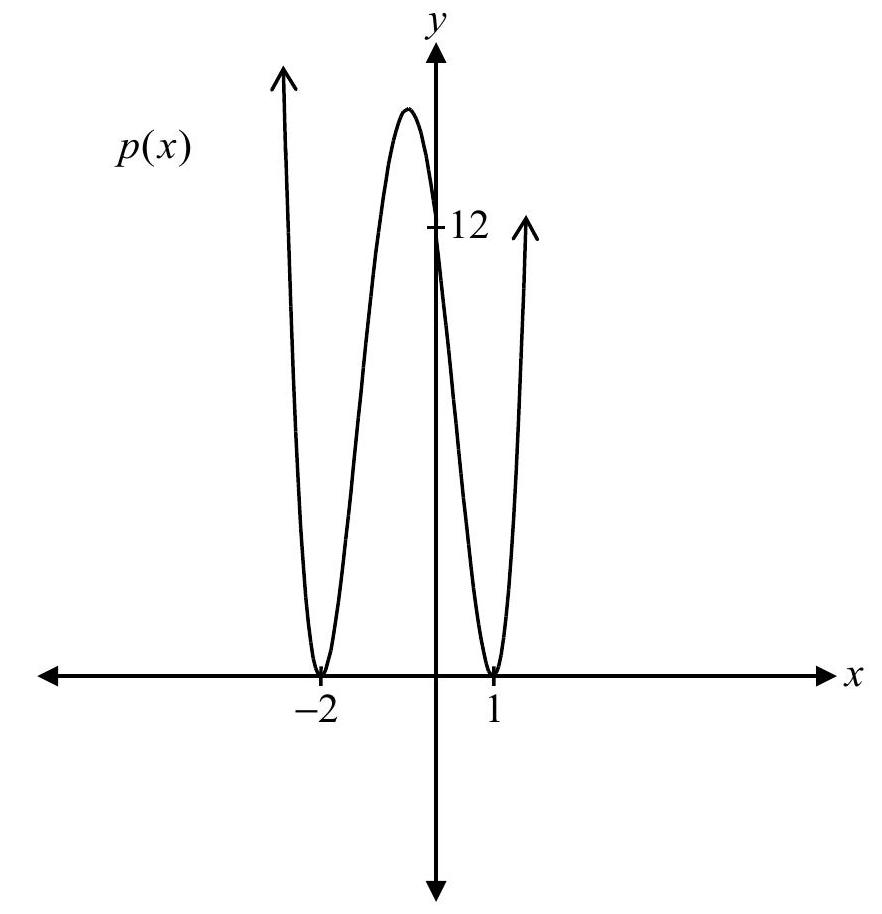
\includegraphics[max width=\textwidth, alt={}, center]{de5fb11a-28c7-4ac7-b7ff-0309cebac724-226_914_882_431_259}\\
$p(x)=$

Evaluate:\\
$\log _{4} 2$

Evaluate:

$$
\left(\cos \frac{11 \pi}{3}\right)\left(\csc \frac{11 \pi}{6}\right)
$$

Estimate the value of $\log _{2} 5$.\\
Justify your answer.

If $\theta$ terminates in quadrant III and $\cos \theta=-\frac{6}{7}$, determine the exact value of $\tan \theta$.

Given $f(x)=x^{2}+x-4$ and $g(x)=\sqrt{x+5}$, Taz was asked to find $f(g(x))$.\\
Taz's solution:

$$
\begin{aligned}
f(g(x)) & =(\sqrt{x+5})^{2}+x-4 \\
& =x+5+x-4 \\
& =2 x+1, x \geq-5
\end{aligned}
$$

Describe the error in Taz's solution.

Sketch the graph of the function $f(x)=3 \log _{2}(x+1)$.\\
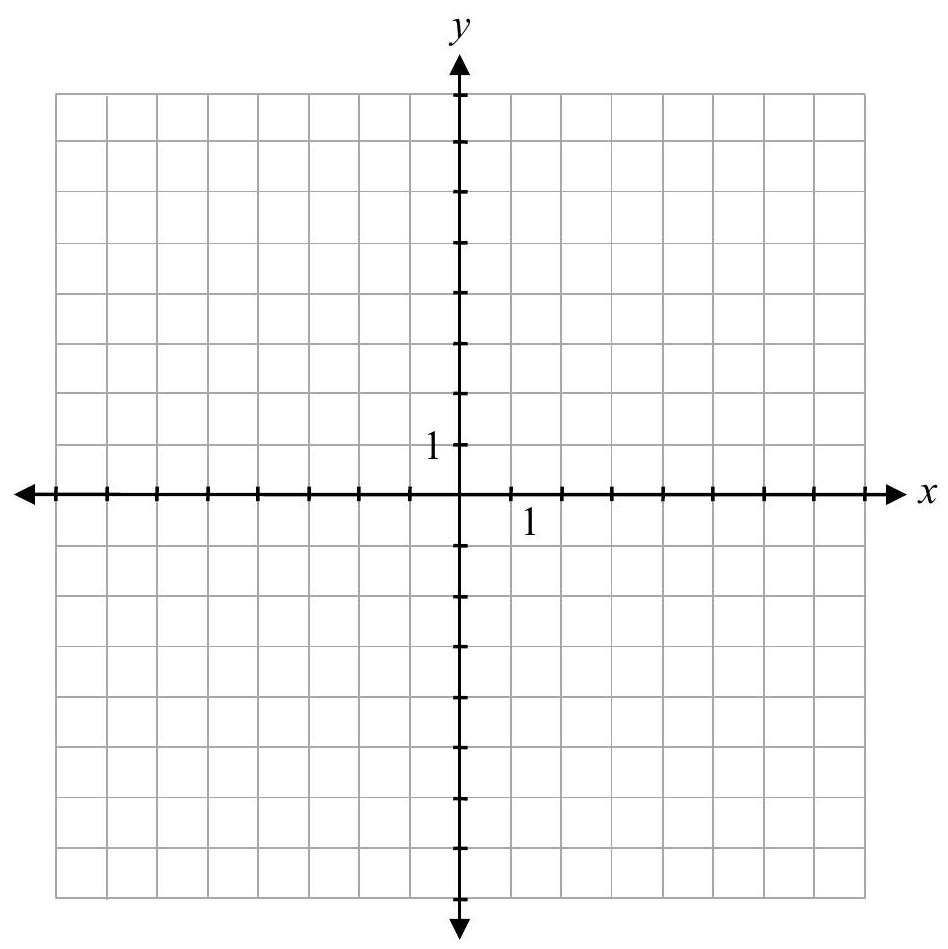
\includegraphics[max width=\textwidth, alt={}, center]{de5fb11a-28c7-4ac7-b7ff-0309cebac724-232_949_948_588_524}

Write an equation of a rational function that would not have any vertical asymptotes.

Determine the exact value of $\tan 75^{\circ}$.

Sketch the graph of the following function:

$$
f(x)=\frac{(x+3)(x-3)}{x(x-3)}
$$

\begin{center}
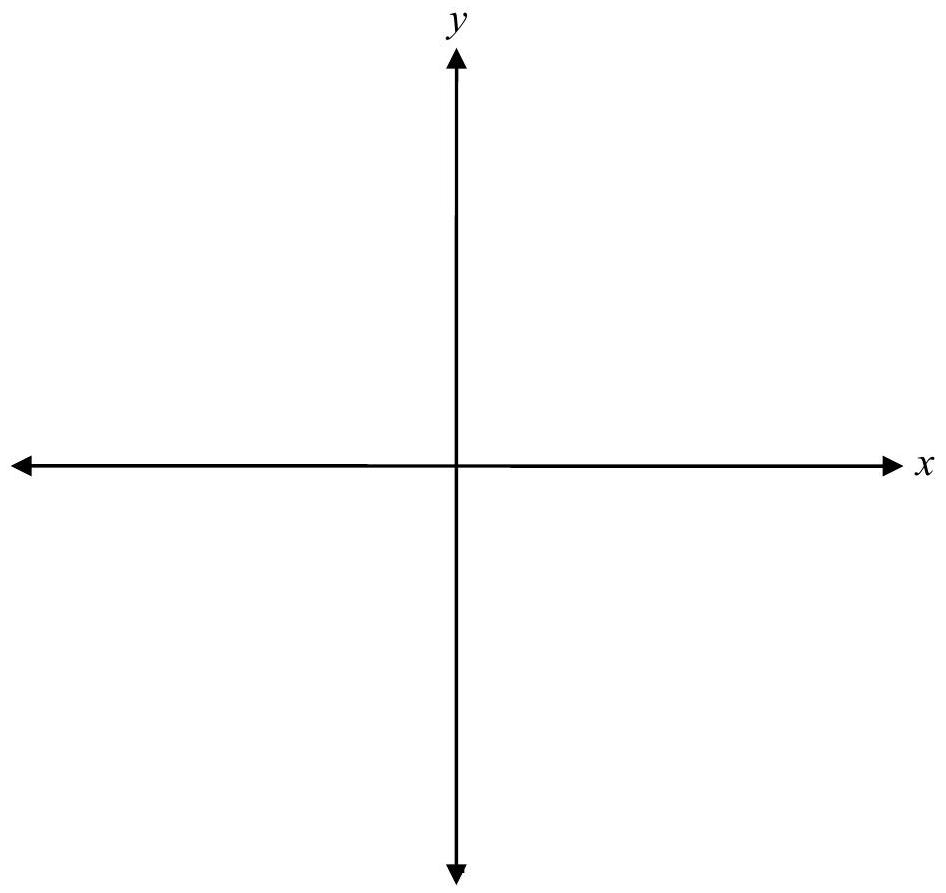
\includegraphics[max width=\textwidth, alt={}]{de5fb11a-28c7-4ac7-b7ff-0309cebac724-235_893_946_657_569}
\end{center}

In the binomial expansion of $\left(\frac{1}{x^{3}}-2 x^{2}\right)^{9}$, determine which term contains $x^{3}$.

José and Dana get on a Ferris wheel, which is 1 metre off the ground. The diameter of the Ferris wheel is 16 metres. Their ride lasts for 4 minutes, in which time the Ferris wheel makes one revolution.

Determine the values of $\mathrm{A}, \mathrm{B}, \mathrm{C}$, and D , if the sinusoidal function that models the situation is $h(t)=A \cos [B(t-C)]+D$, where $h$ is the height at which José and Dana are located on the Ferris wheel, from the ground, in metres, and $t$ is the time, in minutes.\\
$\mathrm{A}=$ $\_\_\_\_$\\
$\mathrm{B}=$ $\_\_\_\_$\\
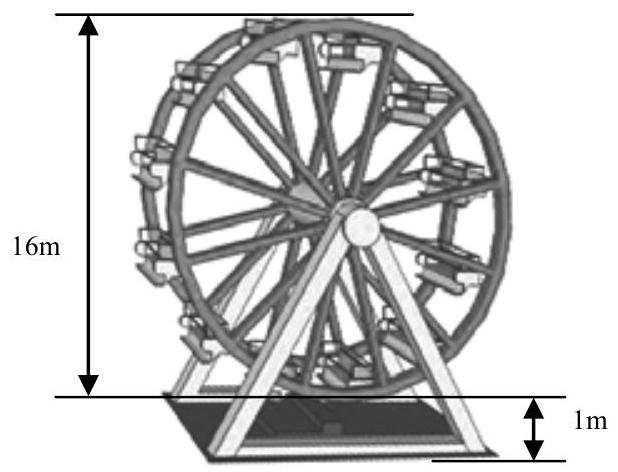
\includegraphics[max width=\textwidth, alt={}, center]{de5fb11a-28c7-4ac7-b7ff-0309cebac724-237_472_618_747_951}\\
$\mathrm{C}=$ $\_\_\_\_$\\
$\mathrm{D}=$ $\_\_\_\_$

Solve algebraically:

$$
{ }_{n} P_{3}=4!(n-1)
$$

Given $f(x)=\frac{2}{x-1}$, determine the equation of the inverse, $f^{-1}(x)$.

Solve:

$$
4 \log _{3} 2-\frac{1}{3} \log _{3} 8=\log _{3} a
$$

Sketch the graph of at least one period of the function $y=3 \cos (\pi x)-1$.\\
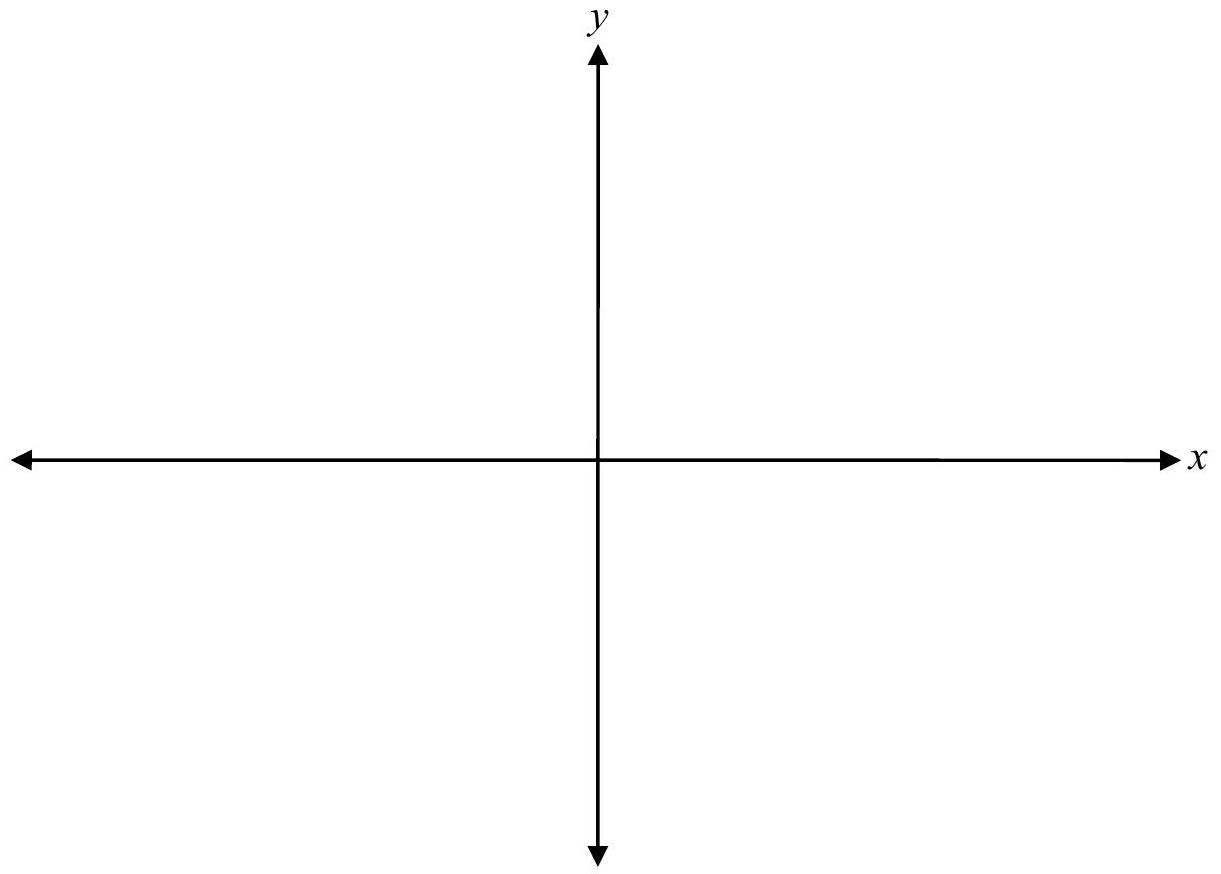
\includegraphics[max width=\textwidth, alt={}, center]{de5fb11a-28c7-4ac7-b7ff-0309cebac724-241_874_1221_534_337}

Using the laws of logarithms, fully expand the expression:

$$
\log _{a}\left(\frac{x^{3}}{y \sqrt{z}}\right)
$$

Sketch the graph of $f(x)=3 \sqrt{x-2}+1$.\\
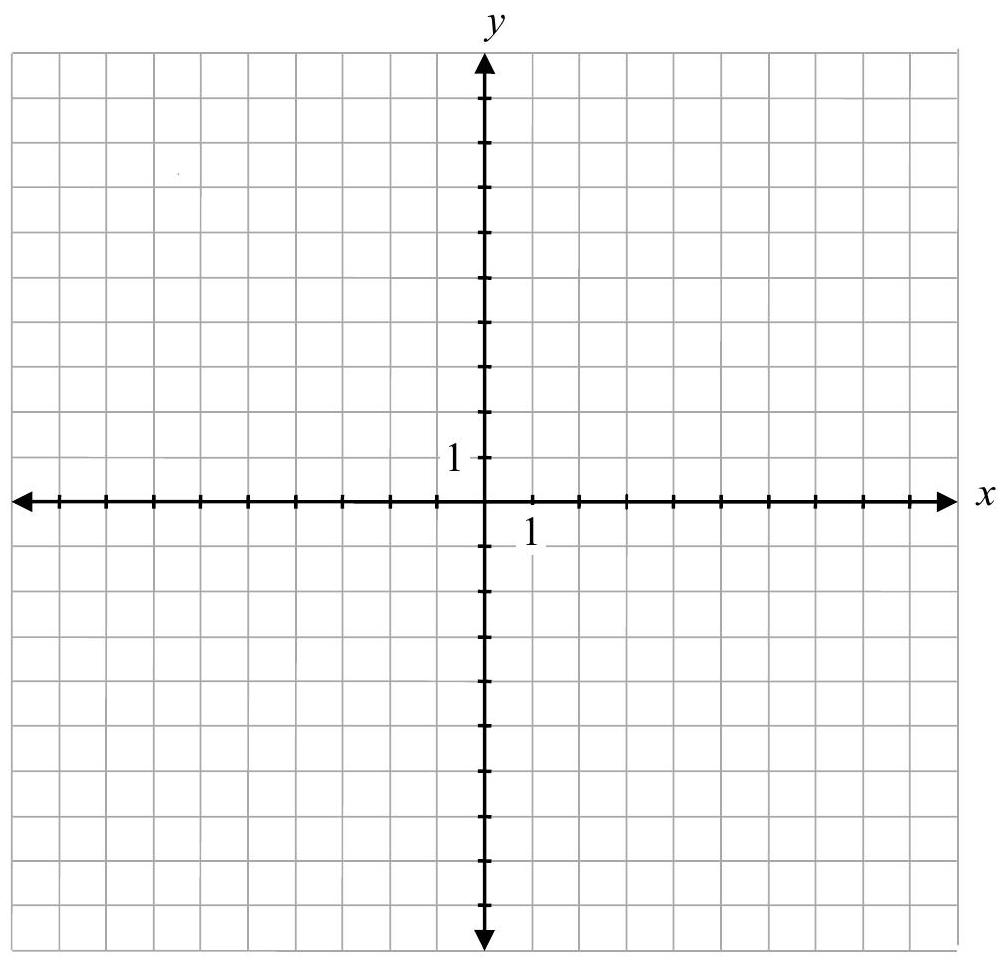
\includegraphics[max width=\textwidth, alt={}, center]{de5fb11a-28c7-4ac7-b7ff-0309cebac724-243_961_1006_595_554}\\
a) Determine the domain of the graph of the function $f(x)=\sqrt{x^{2}-4}$.\\
b) Explain why the domain of $f(x)=\sqrt{x^{2}-4}$ is restricted.

\section*{Question 41}
a) 1 mark b) 1 mark $\quad{ }_{136}^{135}$

Given the point $(-12,-18)$ on the graph of $f(x)$, determine the new points after the following transformations of $f(x)$.\\
a) $\frac{1}{f(x)}$\\
b) $f(-x)+10$

Explain why there is no solution for the equation $\csc \theta=-\frac{1}{2}$.

Given the graph of $y=f(x)$,\\
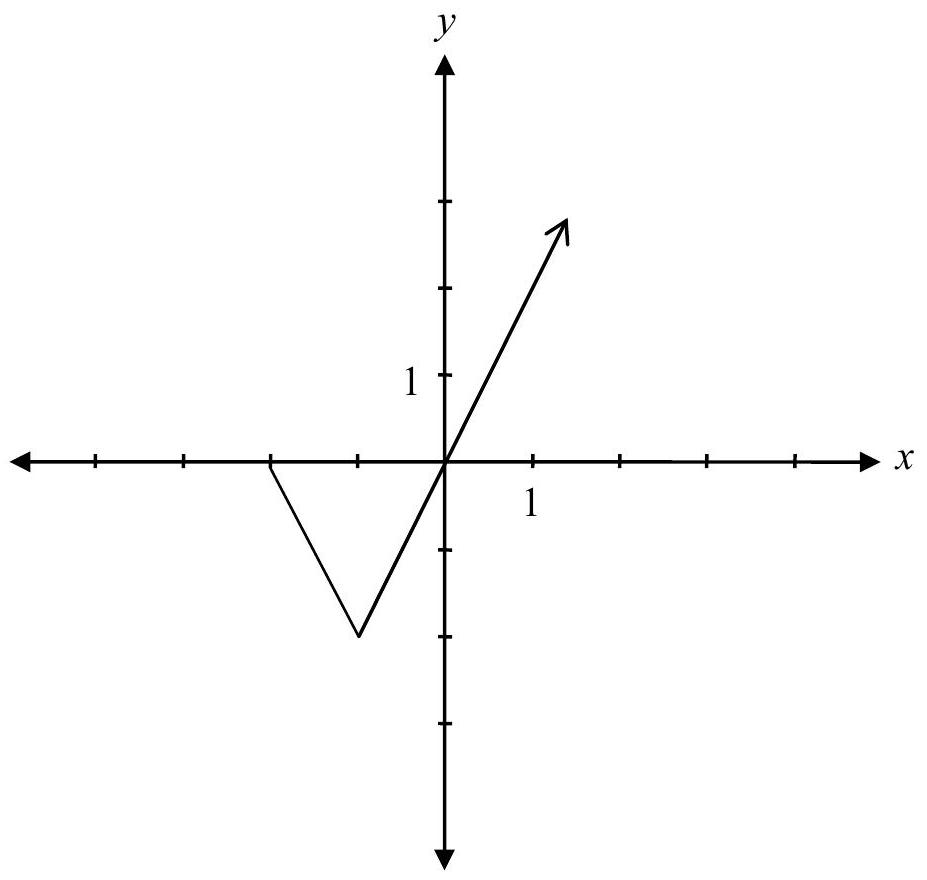
\includegraphics[max width=\textwidth, alt={}, center]{de5fb11a-28c7-4ac7-b7ff-0309cebac724-247_880_927_472_348}\\
sketch the graph of $y=|f(2 x)|+1$.\\
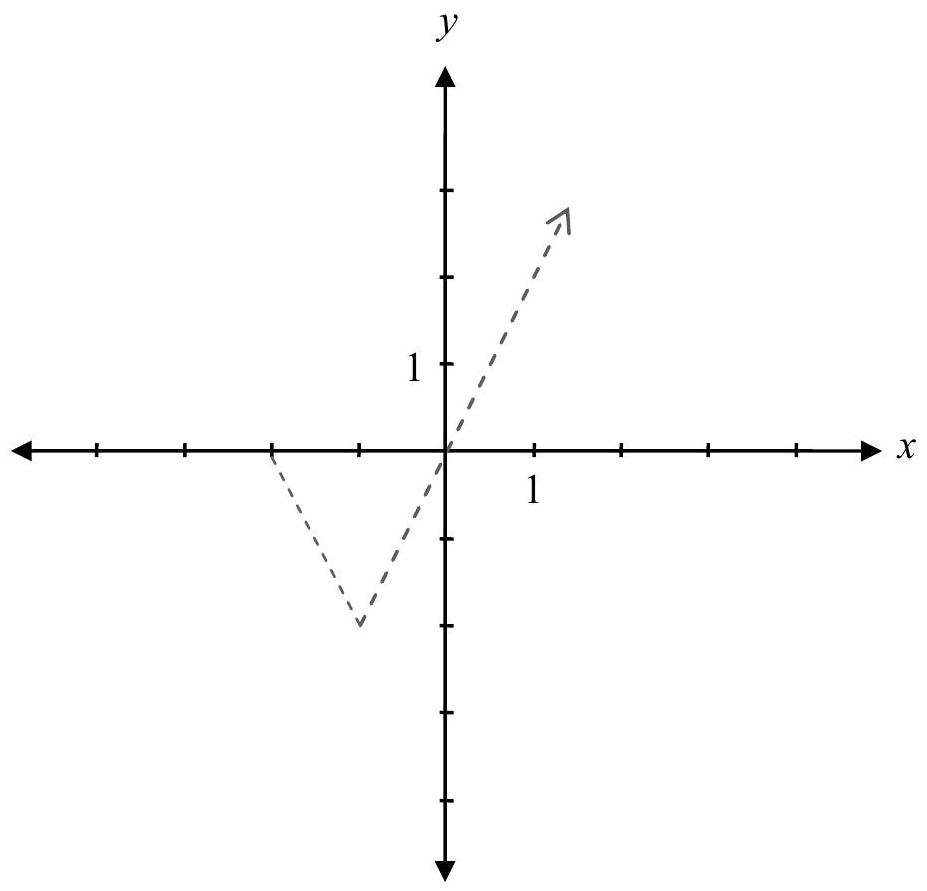
\includegraphics[max width=\textwidth, alt={}, center]{de5fb11a-28c7-4ac7-b7ff-0309cebac724-247_891_927_1574_386}

The graph of $f(x)$ has already been drawn for your reference.

No marks will be awarded for the graph of $f(x)$.

Given $f(x)=2^{x}+1$, state the equation of the horizontal asymptote.

Given the following graphs of $f(x)=x-3$ and $g(x)=x+1$,\\
$f(x)$\\
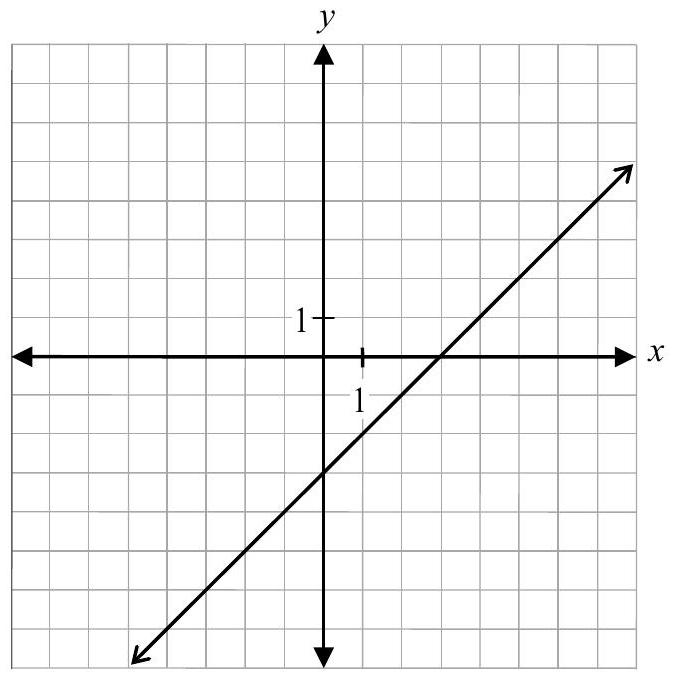
\includegraphics[max width=\textwidth, alt={}, center]{de5fb11a-28c7-4ac7-b7ff-0309cebac724-249_678_676_528_266}\\
$g(x)$\\
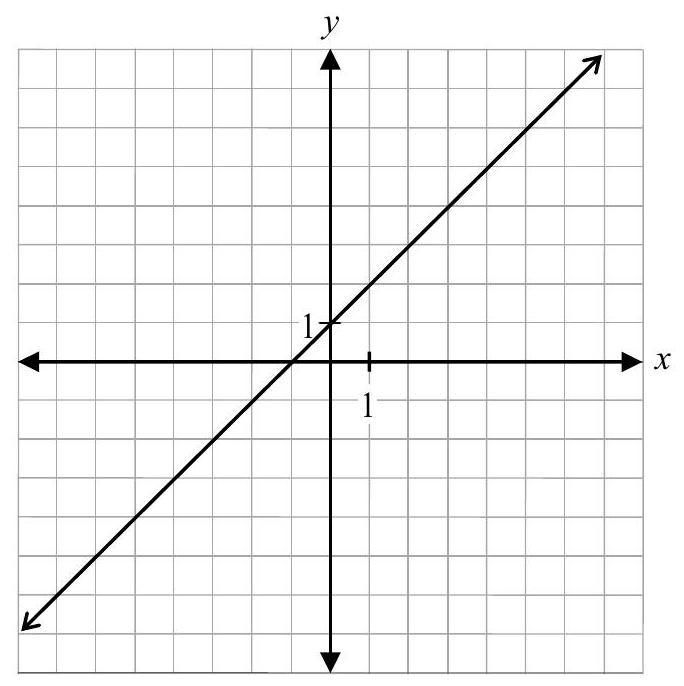
\includegraphics[max width=\textwidth, alt={}, center]{de5fb11a-28c7-4ac7-b7ff-0309cebac724-249_686_684_524_1108}\\
sketch the graph of $h(x)=(f \cdot g)(x)$.\\
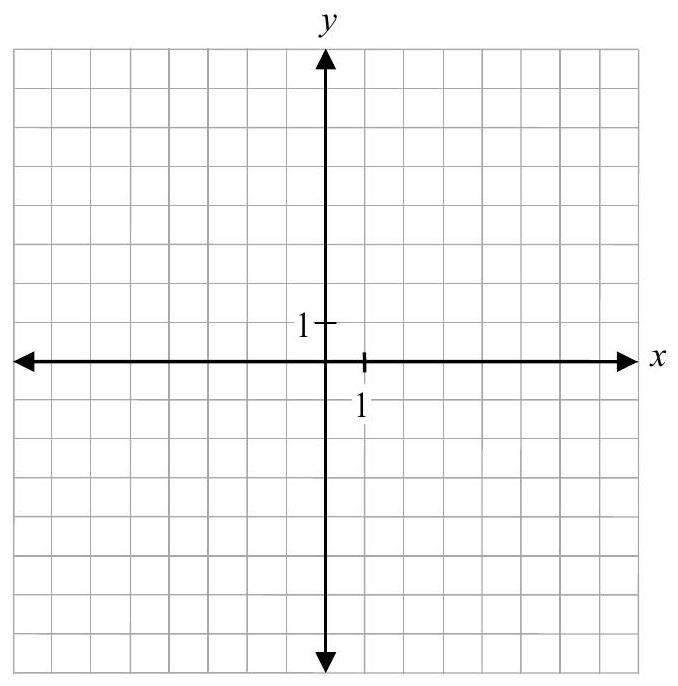
\includegraphics[max width=\textwidth, alt={}, center]{de5fb11a-28c7-4ac7-b7ff-0309cebac724-249_686_678_1482_747}

A wheel has a diameter of 20 cm and rotates through a central angle of $252^{\circ}$.\\
Determine how far the wheel rolled.

Solve the following equation over the interval $[0,2 \pi]$ :

$$
3 \sin ^{2} \theta-10 \sin \theta-8=0
$$

Determine and simplify the fourth term in the expansion of $\left(2 x^{4}-3 y\right)^{8}$.

Sheeva's bank is lending her $\$ 50000$ at an annual interest rate of $6 \%$, compounded monthly, to purchase a car.\\
Given that the last payment will be a partial payment, determine how many full monthly payments of $\$ 800$ Sheeva will have to make.\\
The formula below may be used.

$$
\begin{aligned}
& P V=\frac{R\left[1-(1+i)^{-n}\right]}{i} \\
& \text { where } \quad \begin{aligned}
P V & =\text { the present value of the amount borrowed } \\
R & =\text { the amount of each periodic payment } \\
i & =\frac{\text { annual interest rate (as a decimal) }}{\text { the number of compounding periods per year }} \\
n & =\text { the number of equal periodic payments }
\end{aligned}
\end{aligned}
$$

Express your answer as a whole number.

An employee asked 10 people in an ice cream shop to wait in line.\\
Determine the number of different arrangements possible if two of the people, Jamie and John, refused to stand next to each other in the line.

The point $(-2,4)$ is on the graph of $f(x)$.\\
State the coordinates of the corresponding point when $f(x)$ is reflected over the $y$-axis.

Given the graphs of $f(x)$ and $g(x)$, sketch the graph of $(f+g)(x)$.\\
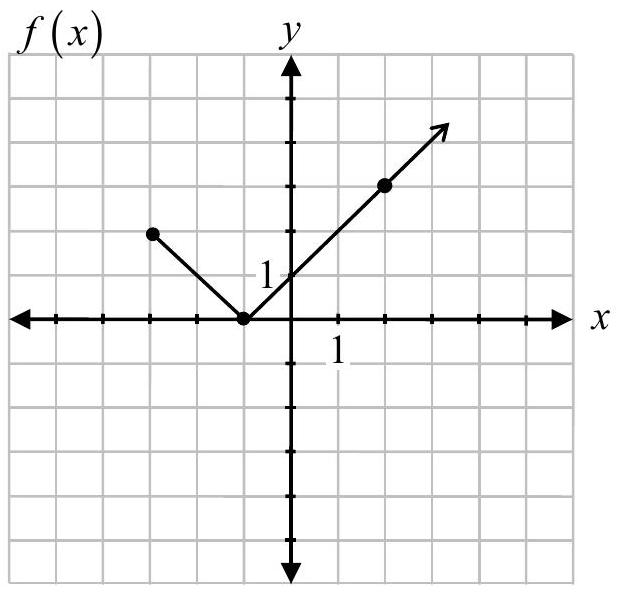
\includegraphics[max width=\textwidth, alt={}, center]{de5fb11a-28c7-4ac7-b7ff-0309cebac724-256_592_622_534_343}\\
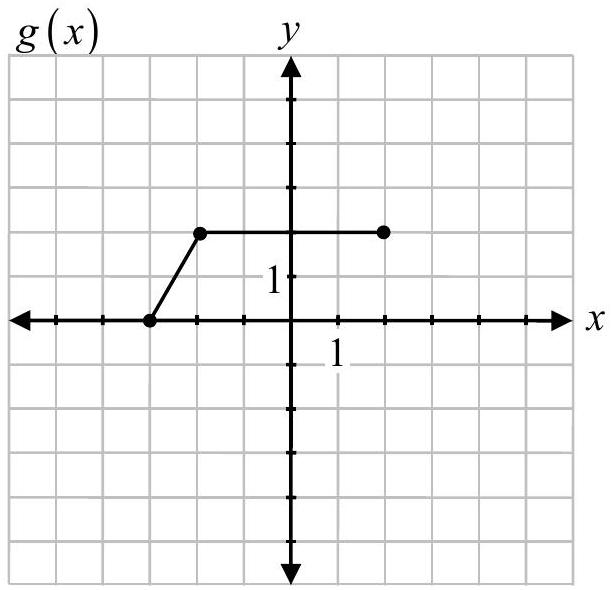
\includegraphics[max width=\textwidth, alt={}, center]{de5fb11a-28c7-4ac7-b7ff-0309cebac724-256_590_613_534_1102}\\
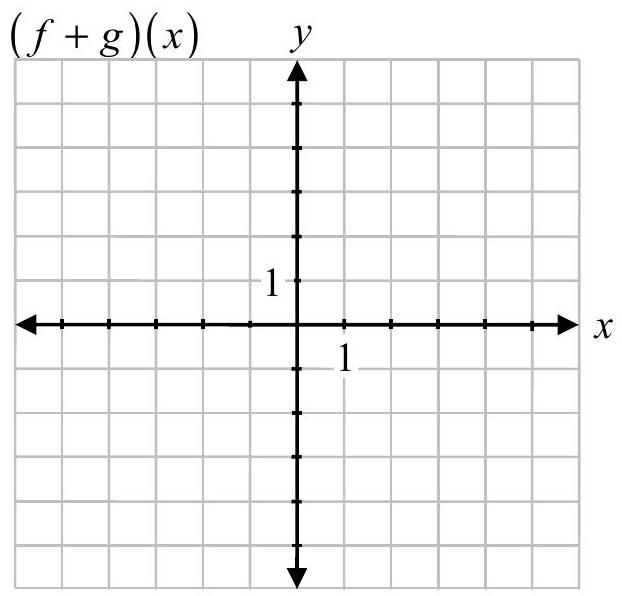
\includegraphics[max width=\textwidth, alt={}, center]{de5fb11a-28c7-4ac7-b7ff-0309cebac724-256_596_622_1299_717}

Using the laws of logarithms, fully expand the expression:

$$
\log _{2}\left(\frac{w^{3} x}{y-1}\right)
$$

Solve the following equation algebraically for $\theta$, where $0 \leq \theta \leq 2 \pi$ :

$$
2 \cos 2 \theta=1
$$

Given the graph of $y=f(x)$, sketch the graph of $y=2|f(x-1)|$.\\
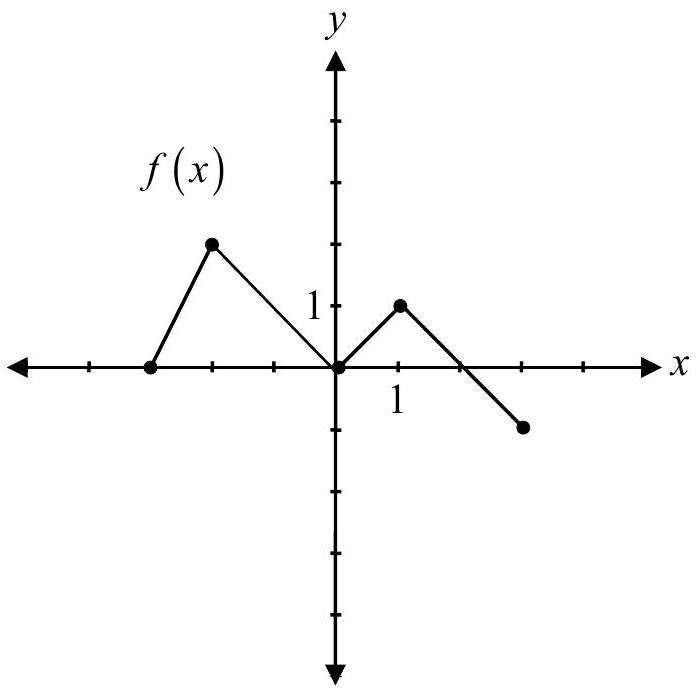
\includegraphics[max width=\textwidth, alt={}, center]{de5fb11a-28c7-4ac7-b7ff-0309cebac724-259_693_699_472_309}\\
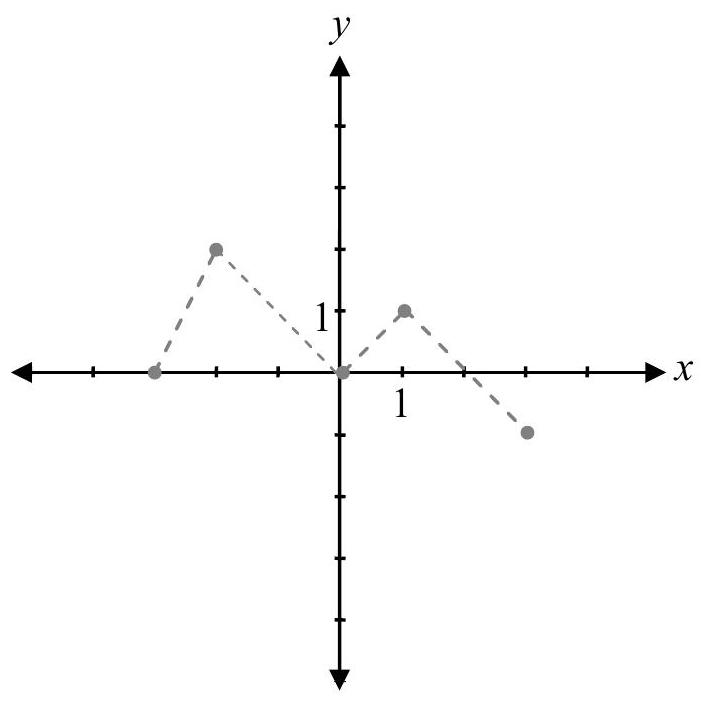
\includegraphics[max width=\textwidth, alt={}, center]{de5fb11a-28c7-4ac7-b7ff-0309cebac724-259_704_708_1314_309}

The graph of $f(x)$ has already been drawn for your reference.

No marks will be awarded for the graph of $f(x)$.

Prove the identity for all permissible values of $\theta$ :

$$
\cos \theta+\tan \theta \sin \theta=\frac{\tan \theta \sin \theta}{1-\cos ^{2} \theta}
$$

\begin{center}
\begin{tabular}{|l|l|}
\hline
Left-Hand Side & Right-Hand Side \\
\hline
\end{tabular}
\end{center}

Raoul has 8 shirts, 5 pairs of pants, and 3 hats. He adds the options together and determines that he has 16 different outfits to wear.\\
Raoul made an error in calculating the number of different outfits. Describe how to determine the correct number of outfits.

Given $f(x)=2 x-1$ and $g(x)=x^{2}+1$ :\\
a) Determine $f(x) \cdot g(x)$.\\
b) Determine $g(g(x))$.

Given the graph of $y=f(x)$, sketch the graph of $y=\sqrt{f(x)}$.\\
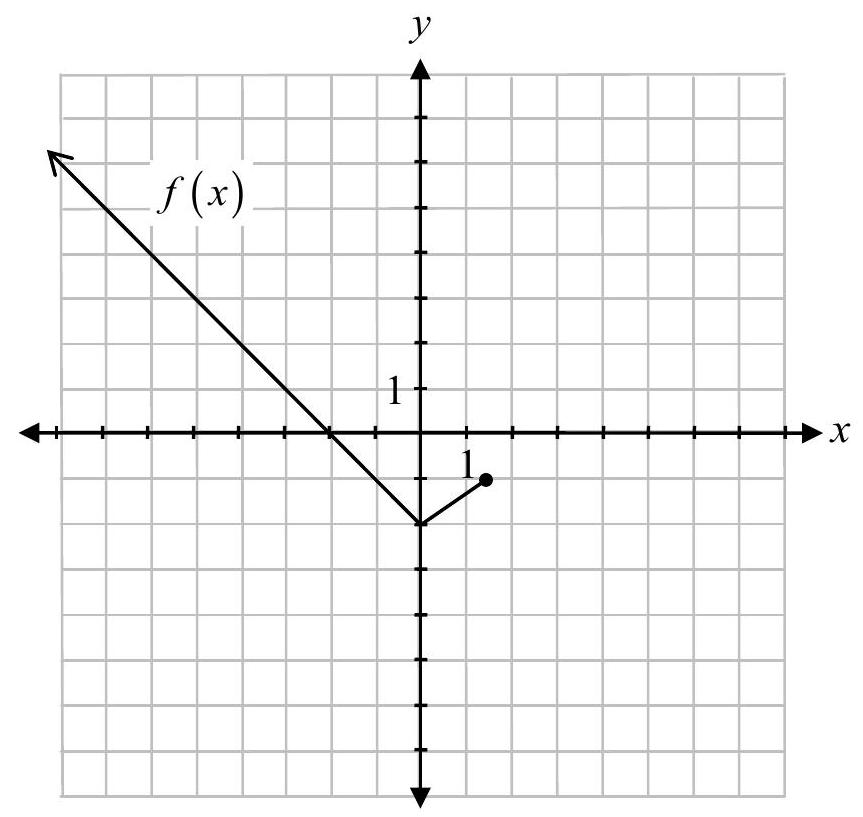
\includegraphics[max width=\textwidth, alt={}, center]{de5fb11a-28c7-4ac7-b7ff-0309cebac724-263_817_863_468_302}\\
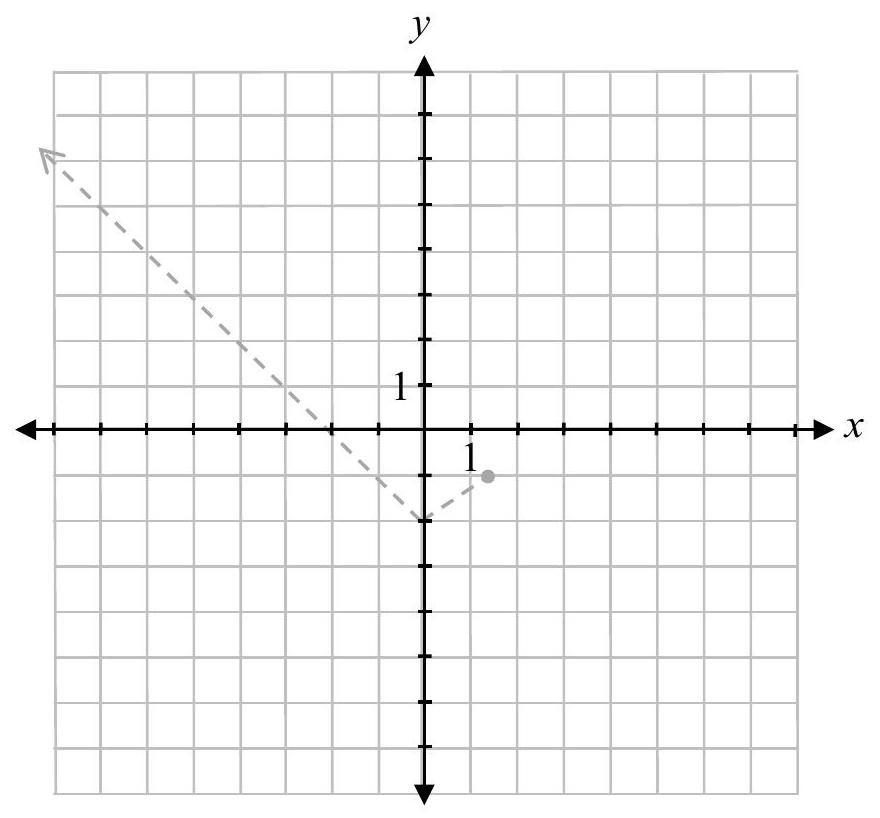
\includegraphics[max width=\textwidth, alt={}, center]{de5fb11a-28c7-4ac7-b7ff-0309cebac724-263_818_880_1445_300}

The graph of $f(x)$ has\\
already been drawn for your reference.\\
No marks will be awarded for the graph of $f(x)$.

Given the polynomial function $P(x)=x^{4}-5 x^{2}-2 x+6$, if $P(1)=0$, identify which statement is true.\\
a) The $y$-intercept is 1 .\\
b) $P(x)$ has a factor of $(x+1)$.\\
c) The graph has a zero at 1 .\\
d) The graph has a zero at -1 .

There are 6 different books that are being distributed evenly amongst three people. Identify which expression represents the number of possible combinations.\\
a) ${ }_{6} C_{2} \cdot{ }_{6} C_{2} \cdot{ }_{6} C_{2}$\\
b) ${ }_{6} C_{2} \cdot{ }_{4} C_{2} \cdot{ }_{2} C_{2}$\\
c) ${ }_{2} C_{2} \cdot{ }_{2} C_{2} \cdot{ }_{2} C_{2}$\\
d) $3 \cdot{ }_{6} C_{2}$

Identify the graph that corresponds to the function $f(x)=-\sqrt{(x-2)}$.\\
a)\\
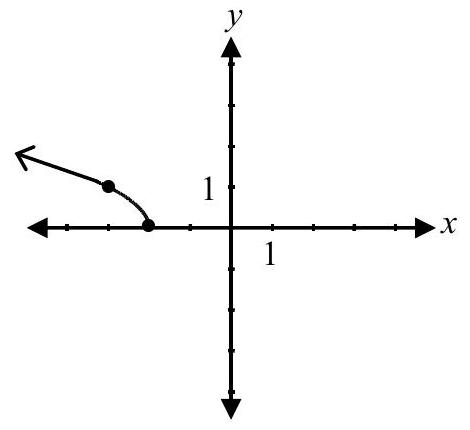
\includegraphics[max width=\textwidth, alt={}, center]{de5fb11a-28c7-4ac7-b7ff-0309cebac724-265_430_470_537_317}\\
b)\\
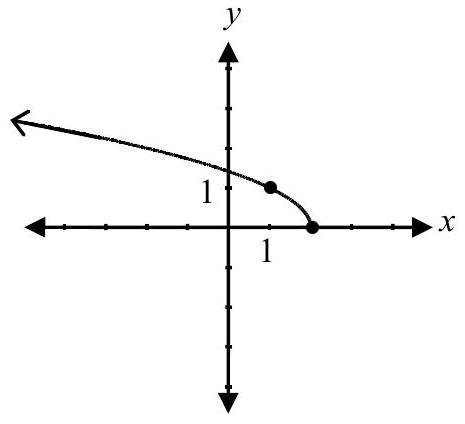
\includegraphics[max width=\textwidth, alt={}, center]{de5fb11a-28c7-4ac7-b7ff-0309cebac724-265_424_465_537_1061}\\
c)\\
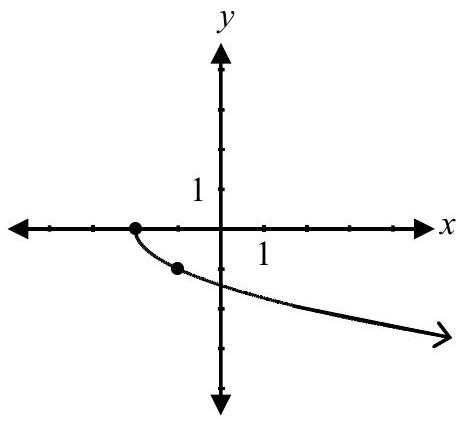
\includegraphics[max width=\textwidth, alt={}, center]{de5fb11a-28c7-4ac7-b7ff-0309cebac724-265_424_467_1061_320}\\
d)\\
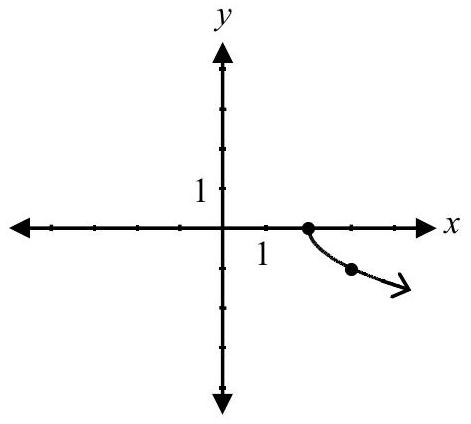
\includegraphics[max width=\textwidth, alt={}, center]{de5fb11a-28c7-4ac7-b7ff-0309cebac724-265_424_471_1052_1074}

Solve:

$$
7^{\log _{7} 2}=x
$$

a) $x=1$\\
b) $x=2$\\
c) $x=7$\\
d) $x=49$

Identify the equation that has a general solution of $\left.\begin{array}{l}\theta=\frac{\pi}{6}+2 \pi k \\ \theta=\frac{5 \pi}{6}+2 \pi k\end{array}\right\}$ where $k \in \mathbb{Z}$.\\
a) $\sin \theta=\frac{1}{2}$\\
b) $\cos \theta=\frac{1}{2}$\\
c) $\sin \theta=\frac{\sqrt{3}}{2}$\\
d) $\cos \theta=\frac{\sqrt{3}}{2}$

Identify the function that has a domain of $x \leq-2$ and a range of $y \geq 3$.\\
a) $y=\sqrt{x+2}+3$\\
b) $y=\sqrt{-(x+2)}+3$\\
c) $y=-\sqrt{x-2}-3$\\
d) $y=-\sqrt{-(x-2)}-3$

Given $f(x)=3 x+2$, identify $f^{-1}(x)$.\\
a) $f^{-1}(x)=-3 x-2$\\
b) $f^{-1}(x)=2 x+3$\\
c) $f^{-1}(x)=\frac{x}{3}-2$\\
d) $f^{-1}(x)=\frac{x-2}{3}$

Identify a possible value for the angle $\theta$ sketched in standard position.\\
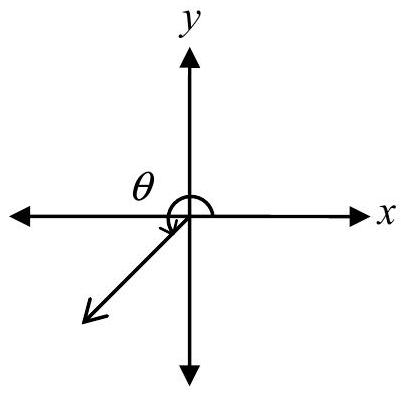
\includegraphics[max width=\textwidth, alt={}, center]{de5fb11a-28c7-4ac7-b7ff-0309cebac724-267_396_405_1626_279}\\
a) 2\\
b) 3\\
c) 4\\
d) 5

Solve the following equation:

$$
\log _{3}(x+3)+\log _{3}(x-5)=2
$$

State a coterminal angle for $\theta=\frac{9 \pi}{4}$.

Sketch the graph of the function $f(x)=\frac{2 x+2}{x^{2}-1}$.\\
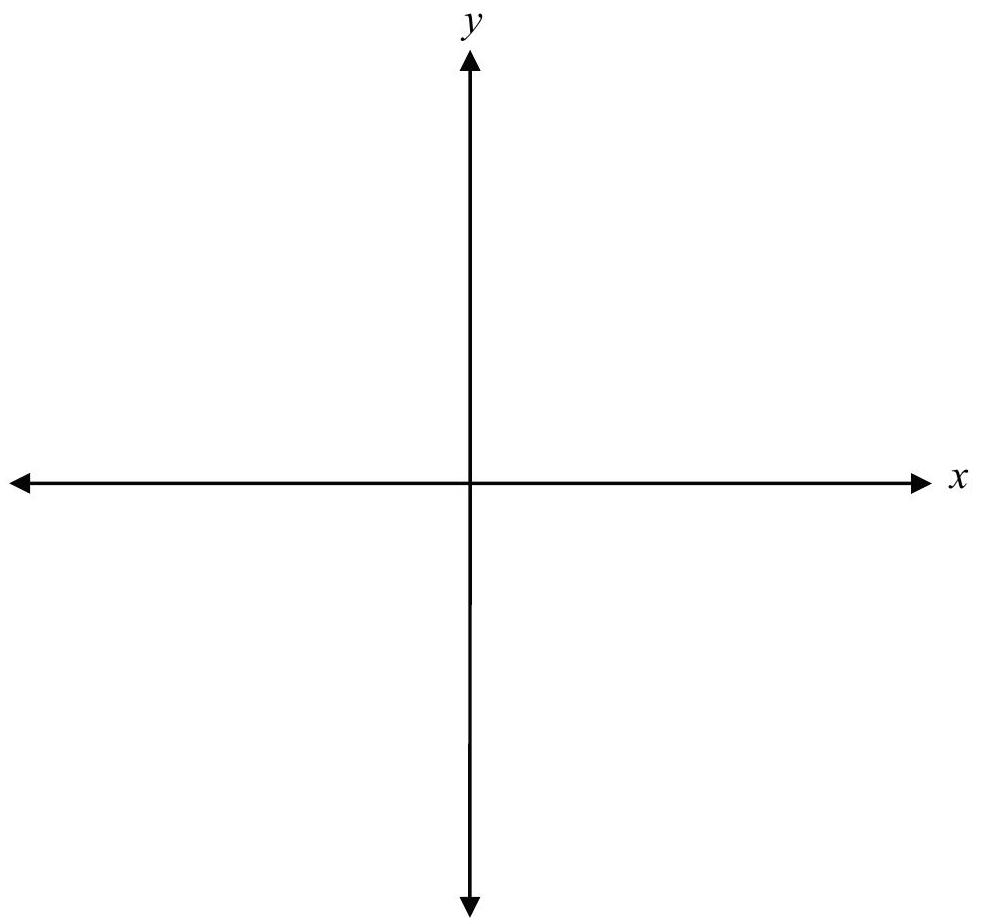
\includegraphics[max width=\textwidth, alt={}, center]{de5fb11a-28c7-4ac7-b7ff-0309cebac724-270_924_981_595_483}

Justify why the binomial expansion of $\left(x+x^{3}\right)^{7}$ does not have a term containing $x^{10}$.

Sketch the graph of $y=-\sin \left(\frac{\pi}{2}(x-1)\right)+3$ over the domain $[0,6]$.\\
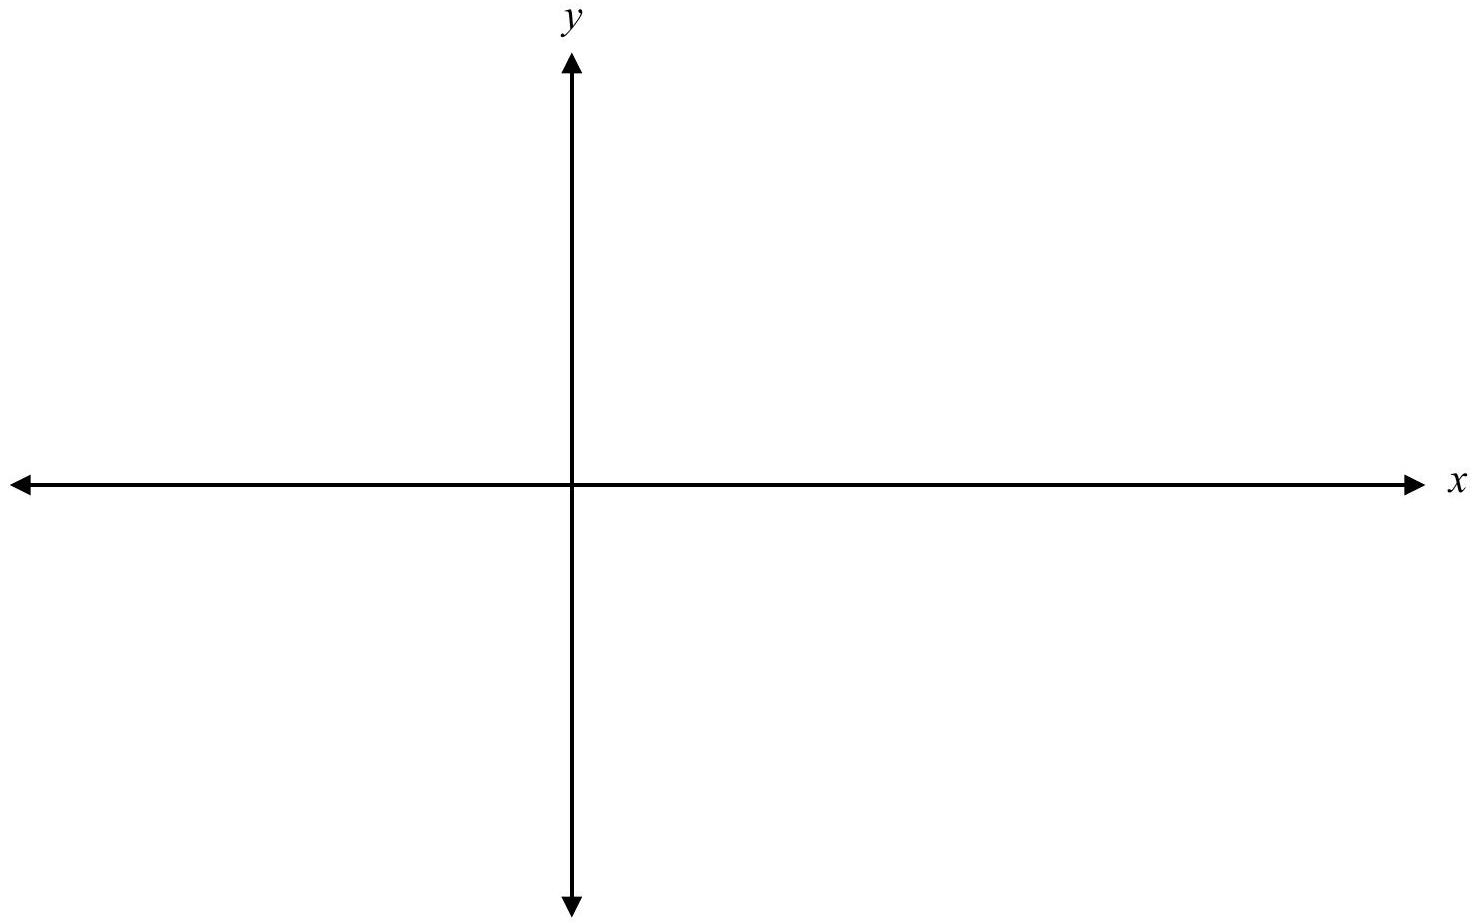
\includegraphics[max width=\textwidth, alt={}, center]{de5fb11a-28c7-4ac7-b7ff-0309cebac724-272_924_1477_653_249}

When $P(x)=3 x^{4}-k x^{3}+5 x-14$ is divided by $(x+2)$, the remainder is -8 .\\
Determine the value of $k$.\\
a) 3 marks\\
b) 1 mark

Given that $\cos \alpha=\frac{7}{12}$ where $\alpha$ is in quadrant IV, and $\sin \beta=\frac{3}{5}$ where $\beta$ is in quadrant I, determine the exact value of:\\
a) $\quad \sin (\alpha-\beta)$\\
b) $\csc (\alpha-\beta)$

Describe the difference between the graph of $f(x)=\frac{7(x+2)}{x+2}$ and the graph of $g(x)=\frac{7(x-2)}{x+2}$ at $x=-2$.

Sketch the graph of $f(x)=3^{x}+2$.\\
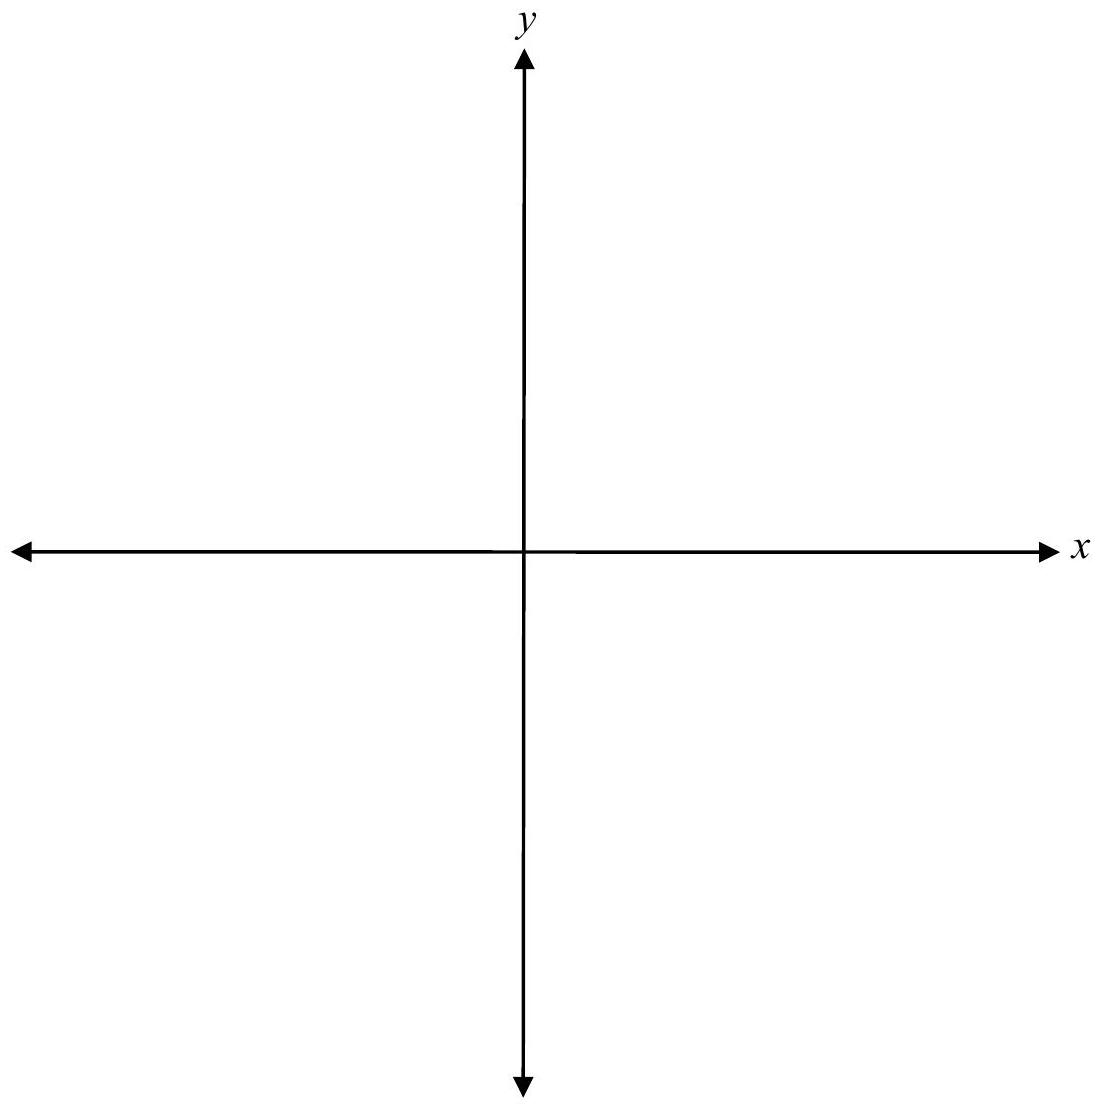
\includegraphics[max width=\textwidth, alt={}, center]{de5fb11a-28c7-4ac7-b7ff-0309cebac724-276_1107_1103_623_436}

Solve algebraically:

$$
{ }_{n} C_{3}=n-2
$$

Describe the error that was made when solving the following equation:

$$
\begin{aligned}
& \sin ^{2} \theta+\sin \theta-2=1 \\
& \sin ^{2} \theta+\sin \theta=3 \\
& \sin \theta(\sin \theta+1)=3 \\
& \sin \theta=3 \quad \sin \theta+1=3 \\
& \begin{array}{l}
\text { sin } \theta=2 \\
\text { ∴ No solution } \quad \therefore \text { No solution }
\end{array}
\end{aligned}
$$

Sketch the graph of the polynomial function with the following characteristics.

\begin{itemize}
  \item a $y$-intercept of -9
  \item zeroes at -1 and 3
  \item the zero at -1 has a multiplicity of 1 and the zero at 3 has a multiplicity of 2\\
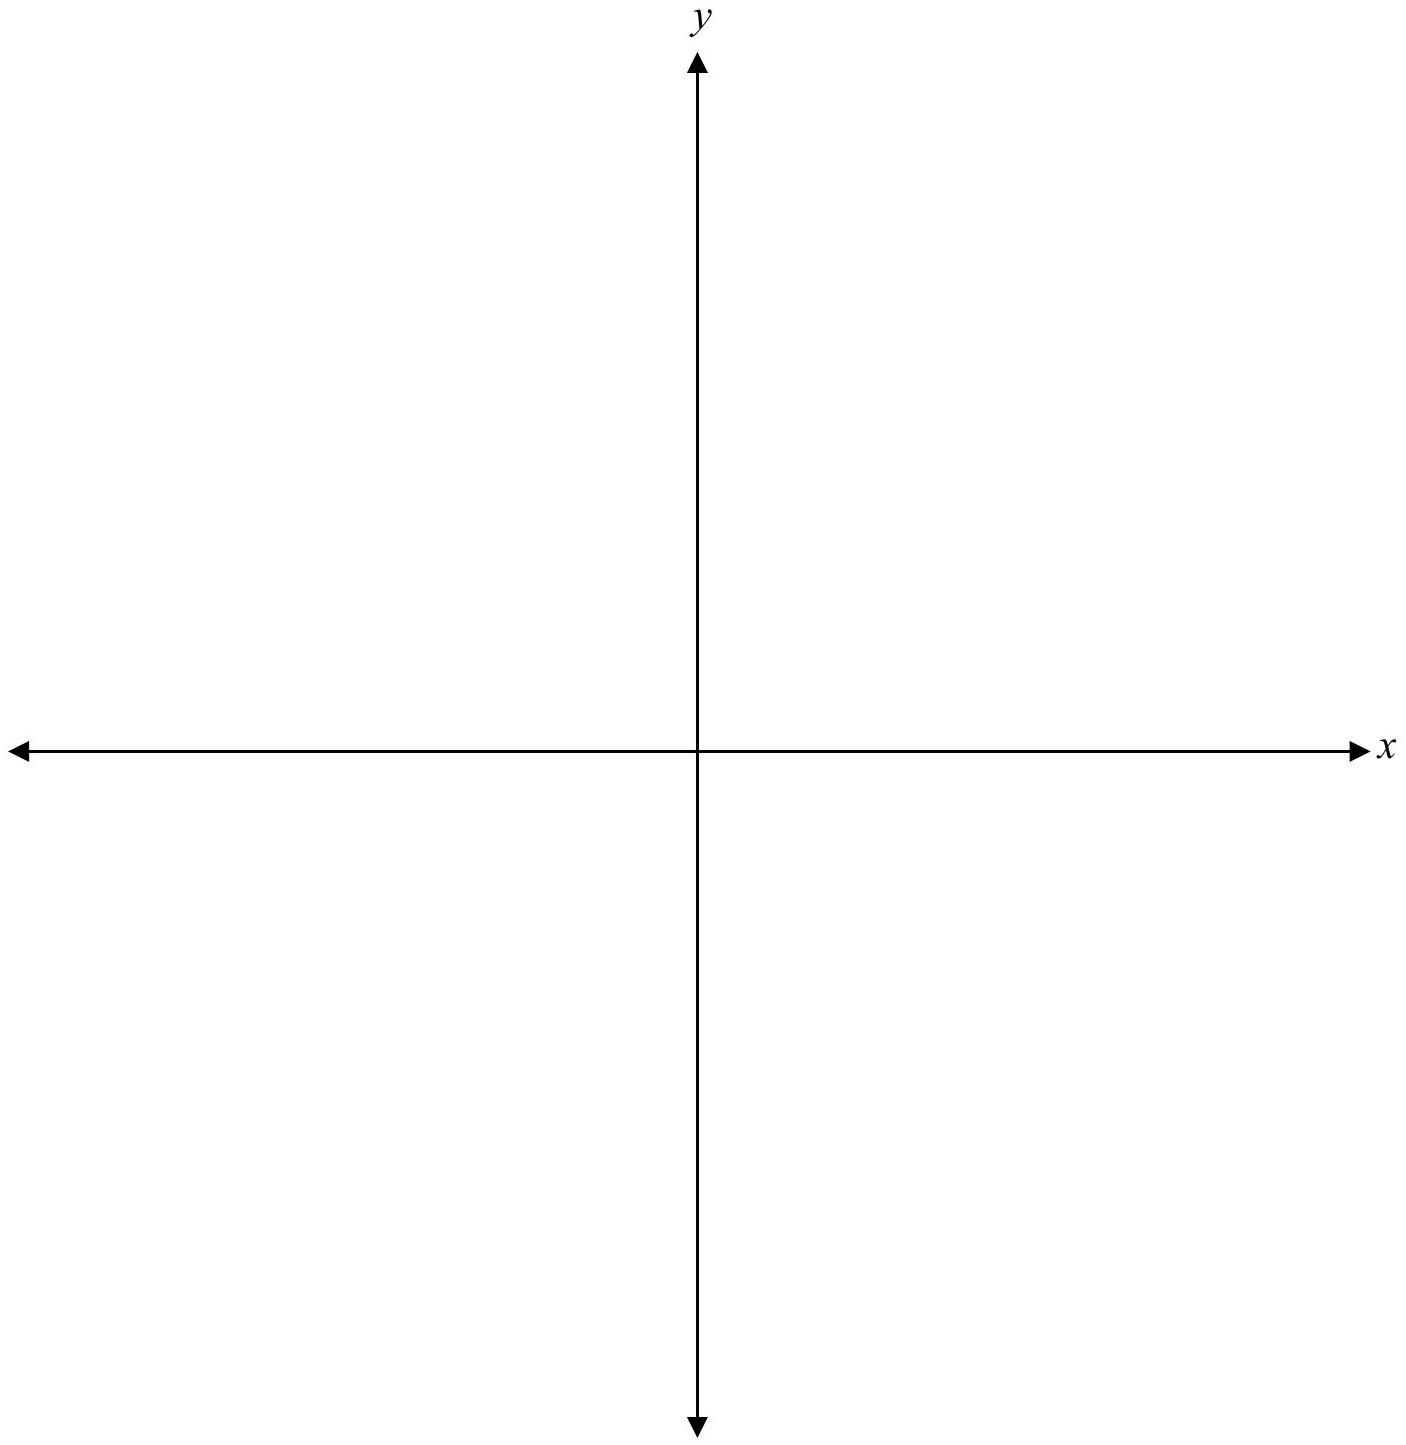
\includegraphics[max width=\textwidth, alt={}, center]{de5fb11a-28c7-4ac7-b7ff-0309cebac724-279_1445_1406_713_309}
\end{itemize}

Given $\cot \theta=-\frac{1}{3}$, where $\theta$ is in quadrant II, determine the exact value of $\sin \theta$.

Given the function $f(x)$, sketch the graph of the reciprocal, $\frac{1}{f(x)}$.\\
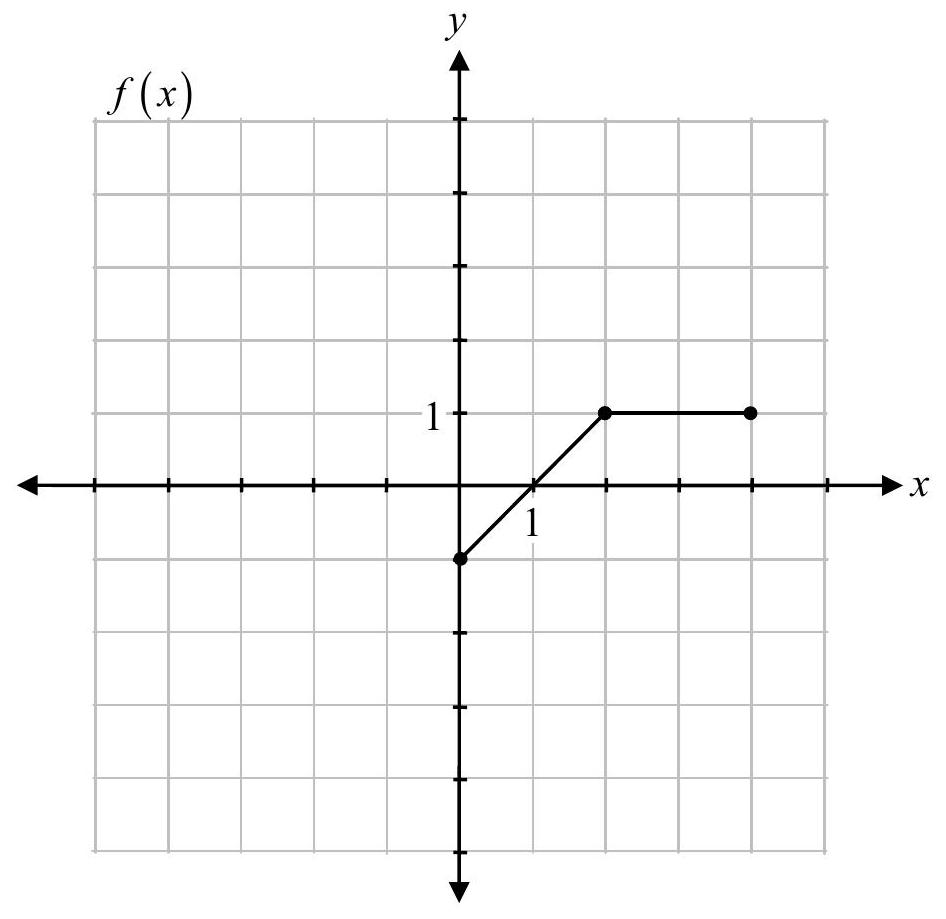
\includegraphics[max width=\textwidth, alt={}, center]{de5fb11a-28c7-4ac7-b7ff-0309cebac724-281_919_946_517_571}\\
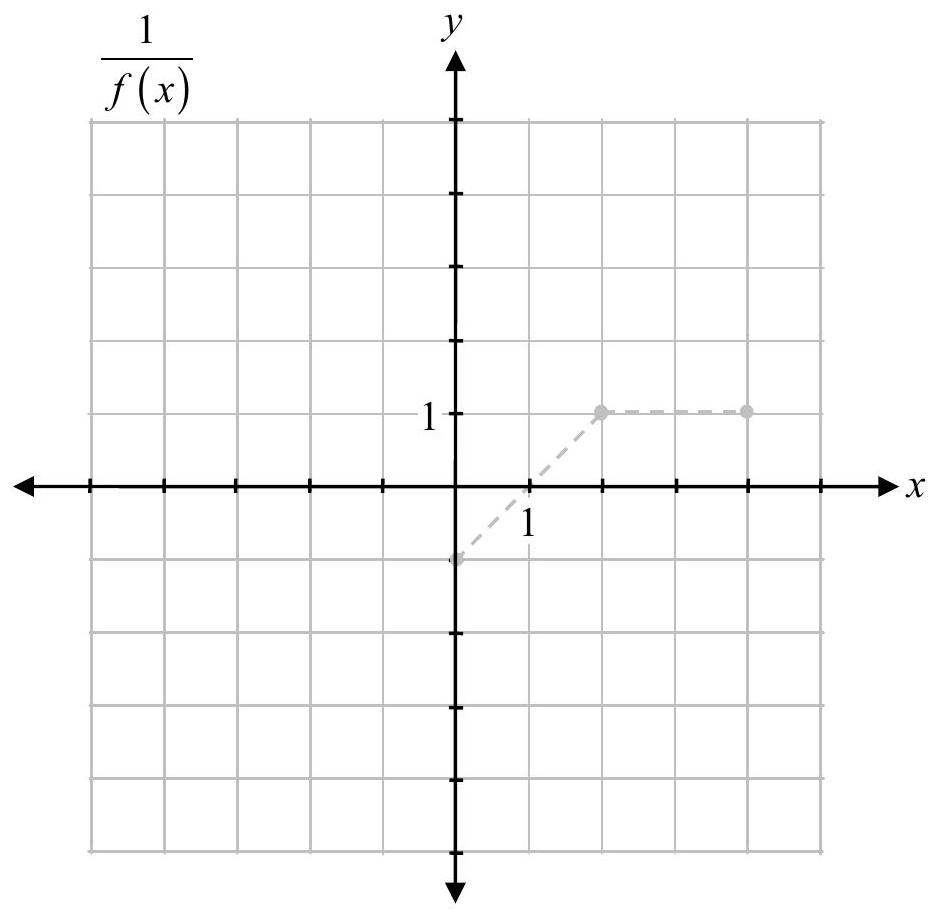
\includegraphics[max width=\textwidth, alt={}, center]{de5fb11a-28c7-4ac7-b7ff-0309cebac724-281_914_935_1555_367}

The graph of $f(x)$ has already been drawn for your reference.\\
No marks will be awarded for the graph of $f(x)$.

The volume of a planter, in the shape of a rectangular prism, can be modelled by the polynomial function $V(x)=x^{3}+3 x^{2}-34 x+48$.\\
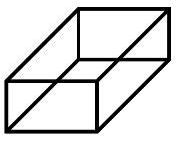
\includegraphics[max width=\textwidth, alt={}, center]{de5fb11a-28c7-4ac7-b7ff-0309cebac724-282_141_179_369_1624}

Determine the factors of the function, $V(x)$, which represent possible dimensions of this planter.\\
$V(x)=$ $\_\_\_\_$

Describe how to determine the range of the inverse of the following graph.\\
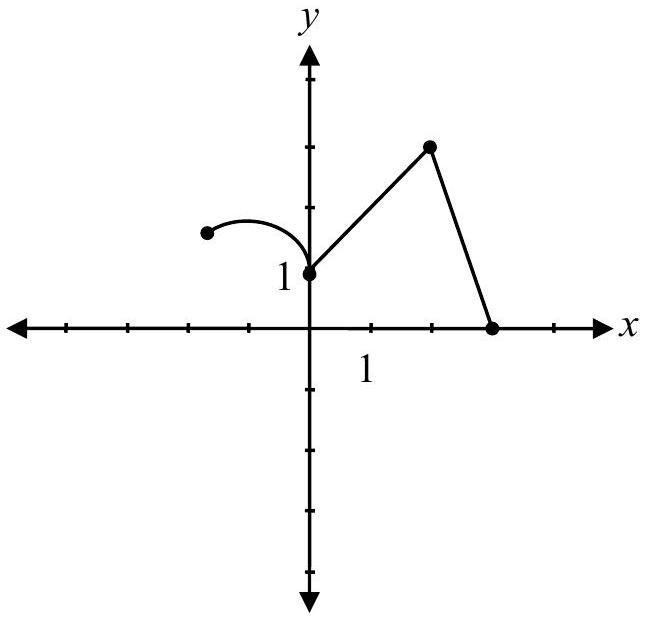
\includegraphics[max width=\textwidth, alt={}, center]{de5fb11a-28c7-4ac7-b7ff-0309cebac724-283_617_646_507_328}

Sketch the graph of the function $y=\sqrt{2 x}+1$.\\
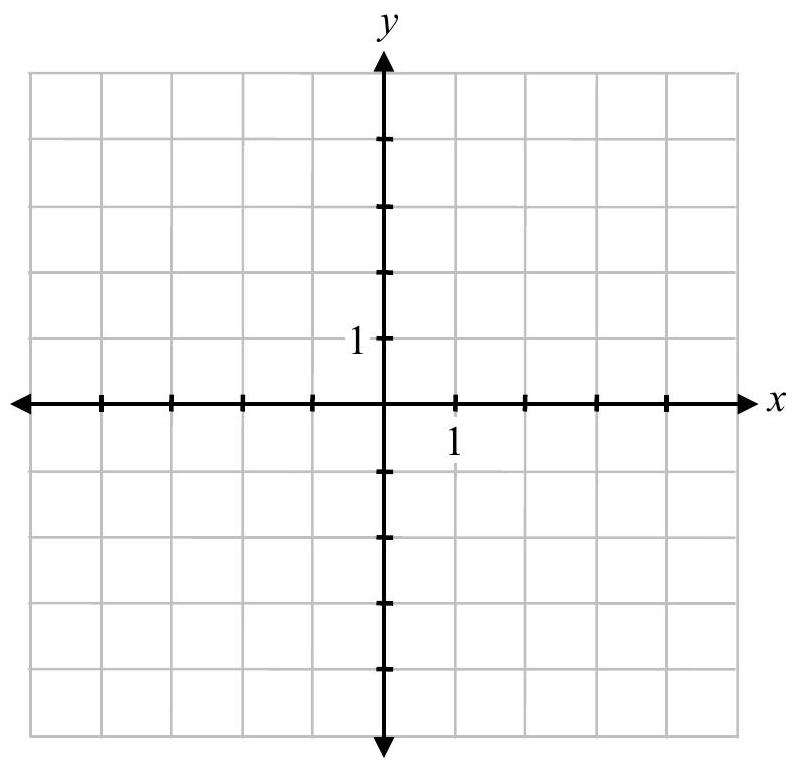
\includegraphics[max width=\textwidth, alt={}, center]{de5fb11a-28c7-4ac7-b7ff-0309cebac724-284_768_796_526_590}

Given the following characteristics of a sinusoidal function:

\begin{itemize}
  \item an amplitude of 2
  \item a vertical translation down 3 units
  \item a period of $\frac{\pi}{4}$\\
a) Determine an equation of this sinusoidal function in the form $y=a \sin b(x-c)+d$.\\
b) Determine the range of this function.
\end{itemize}

Range:

Suah was given the graph of $f(x)$ and asked to graph $y=\sqrt{f(x)}$.\\
Her solution is given on the graph below.\\
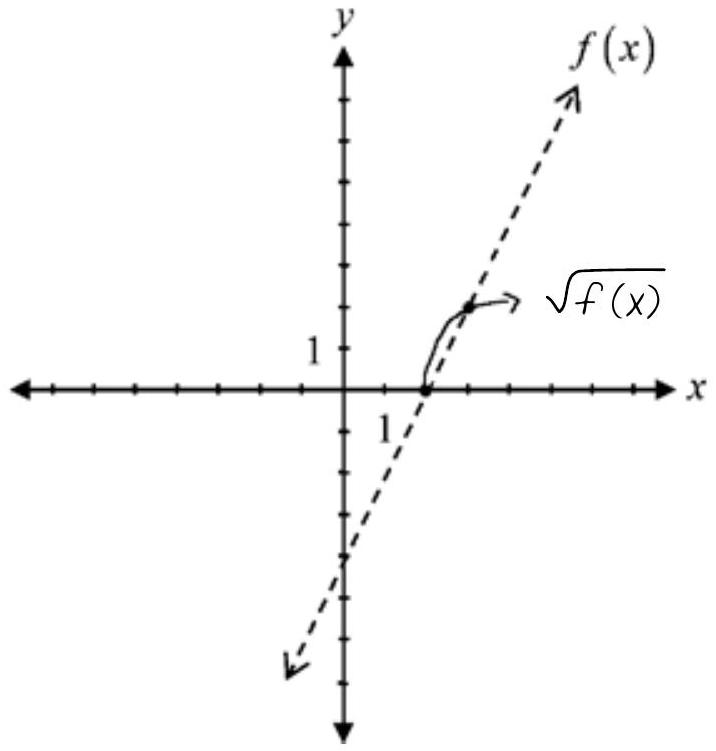
\includegraphics[max width=\textwidth, alt={}, center]{de5fb11a-28c7-4ac7-b7ff-0309cebac724-286_751_716_586_262}

Describe the error Suah made when sketching the graph of $y=\sqrt{f(x)}$.

Solve:

$$
9^{2 x+1}=27^{x}
$$

There are 24 different movies Kiandra can download to her computer. Determine the number of ways she can select 15 movies.

Given $\theta=40^{\circ}$,\\
a) convert $\theta$ to radians.\\
b) determine the coterminal angles of $\theta$ where $\theta \in \mathbb{R}$.

Peter invests $\$ 560$ per month at an annual interest rate of $4.2 \%$, compounded monthly. Determine how many monthly investments he will need to make to obtain at least $\$ 500000$.

Express your answer as a whole number.\\
Use the formula:

$$
\mathrm{FV}=\frac{\mathrm{R}\left[(1+i)^{n}-1\right]}{i}
$$

where $\mathrm{FV}=$ the future value\\
$\mathrm{R}=$ the investment amount each period\\
$i=\frac{\text { the annual interest rate }}{\text { the number of compounding periods per year }}$\\
$n=$ the number of investments

Ishmael has 4 dogs, 5 cats, and 3 horses.\\
If he arranges all of them in a row, determine how many ways they can be arranged if each type of animal must be grouped together.

Solve the following equation algebraically over the interval $0 \leq \theta \leq 2 \pi$.

$$
2 \cos ^{2} \theta+9 \cos \theta-5=0
$$

Determine which term contains $\frac{1}{x^{6}}$ in the binomial expansion of $\left(\frac{2}{x^{3}}+3 x^{2}\right)^{7}$.

Determine the radius of a circle which has an arc length of 5 cm with a central angle of 3 radians.

Tyler incorrectly sketched the angle $\theta=-\frac{7 \pi}{4}$ in standard position.\\
Describe his error.\\
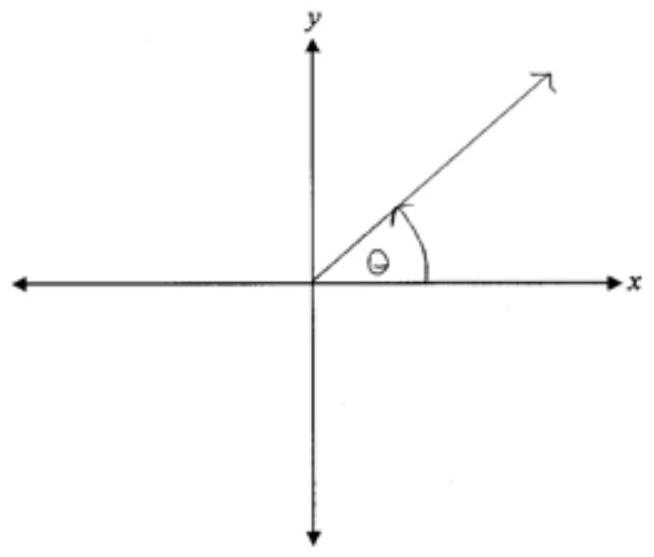
\includegraphics[max width=\textwidth, alt={}, center]{de5fb11a-28c7-4ac7-b7ff-0309cebac724-295_557_654_653_225}

\section*{Question 9}
Given the identity $\sec \theta+\cos \theta=\frac{2-\sin ^{2} \theta}{\cos \theta}$,\\
a) determine the non-permissible values of $\theta$, over the interval $0 \leq \theta \leq 2 \pi$.\\
b) prove the identity for all permissible values of $\theta$.

\begin{center}
\begin{tabular}{|l|l|}
\hline
Left-Hand Side & Right-Hand Side \\
\hline
\end{tabular}
\end{center}

Expand using the laws of logarithms.

$$
\log \left(\frac{a}{b^{4}}\right)
$$

State the equation of $g(x)$ in terms of $f(x)$.\\
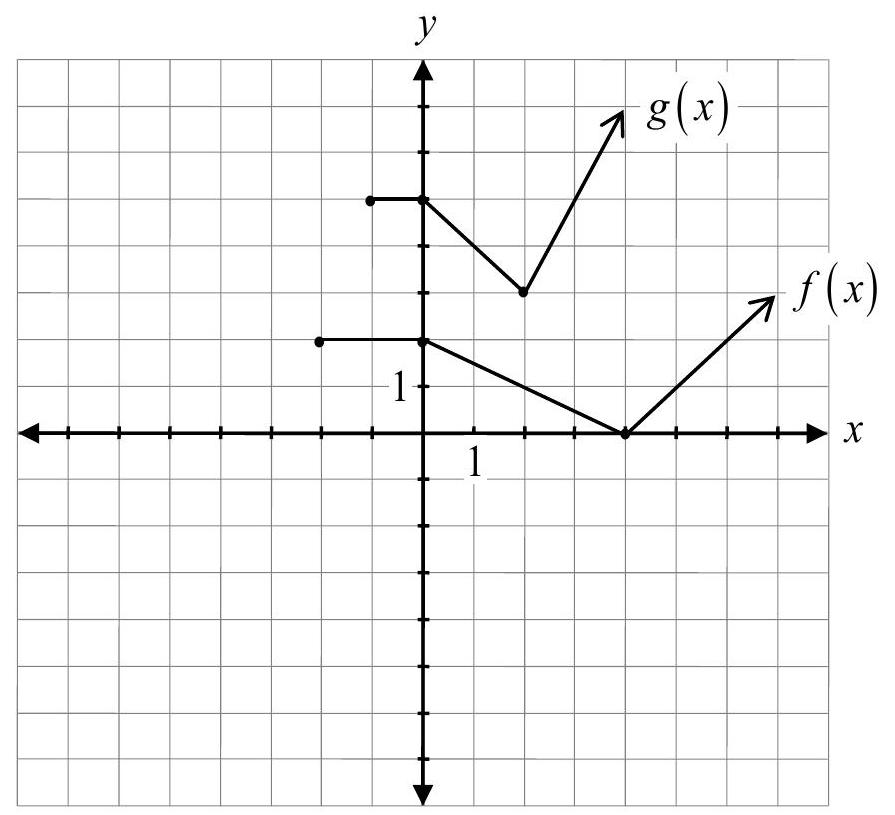
\includegraphics[max width=\textwidth, alt={}, center]{de5fb11a-28c7-4ac7-b7ff-0309cebac724-298_815_895_468_193}

$$
g(x)=
$$

$\_\_\_\_$

Explain why the inverse of the graph of $y=f(x)$ is not a function.\\
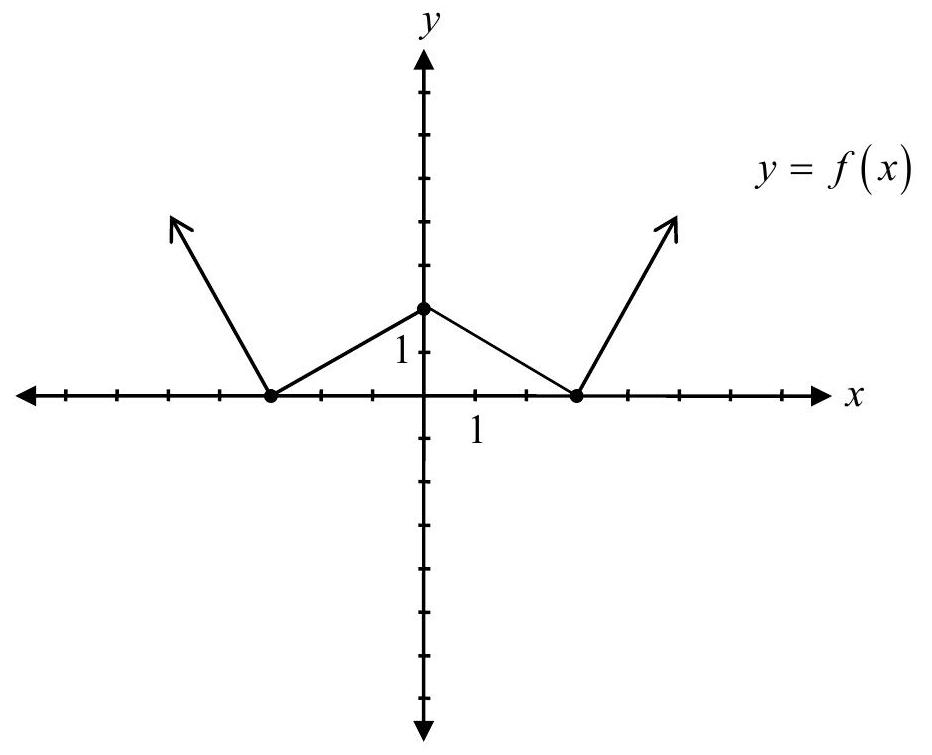
\includegraphics[max width=\textwidth, alt={}, center]{de5fb11a-28c7-4ac7-b7ff-0309cebac724-299_755_932_451_227}

Solve the following equation algebraically:

$$
\log \left(x^{2}+5\right)-\log \left(x^{2}+1\right)=\log 3
$$

Describe the transformations used to obtain the graph of the function $y=5 f(x+1)$ from the graph of $y=f(x)$.

Solve algebraically:

$$
{ }_{n} C_{2}=3 n+4
$$

Given the graph of $f(x)$, sketch the graph of $y=\left|\frac{1}{2} f(x-1)\right|$.\\
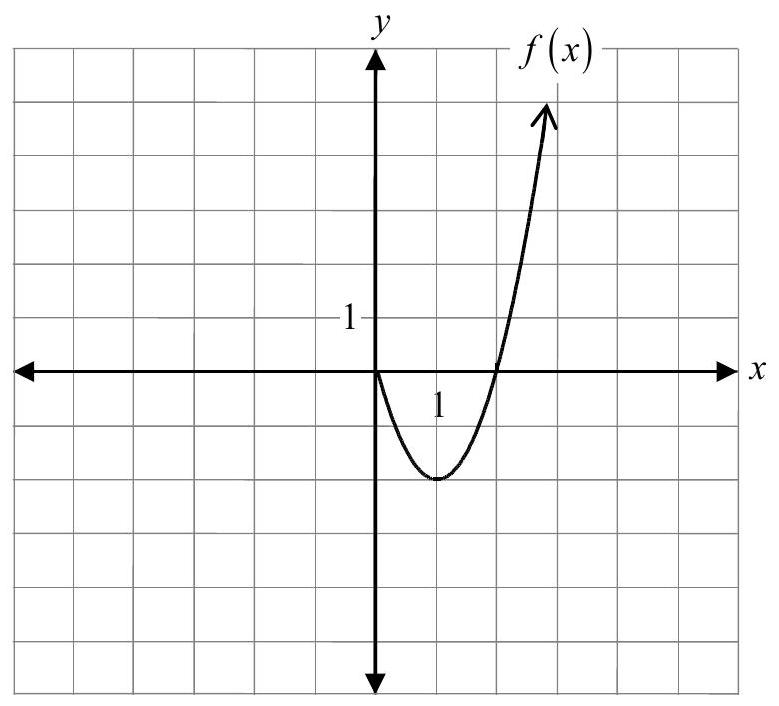
\includegraphics[max width=\textwidth, alt={}, center]{de5fb11a-28c7-4ac7-b7ff-0309cebac724-303_706_779_489_225}\\
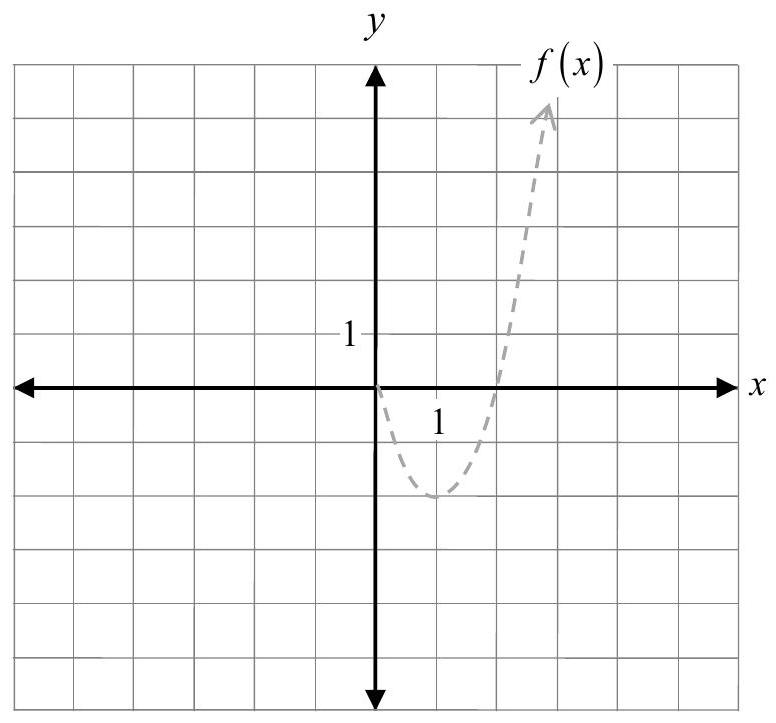
\includegraphics[max width=\textwidth, alt={}, center]{de5fb11a-28c7-4ac7-b7ff-0309cebac724-303_723_776_1336_335}

The graph of $f(x)$ has already been drawn for your reference.\\
No marks will be awarded for the graph of $f(x)$.

Explain why $f(x)=(x+2)^{3}(x-1)^{\frac{1}{2}}$ is not a polynomial function.

Given the graphs of $f(x)$ and $g(x)$, sketch the graph of $h(x)=(f \cdot g)(x)$.\\
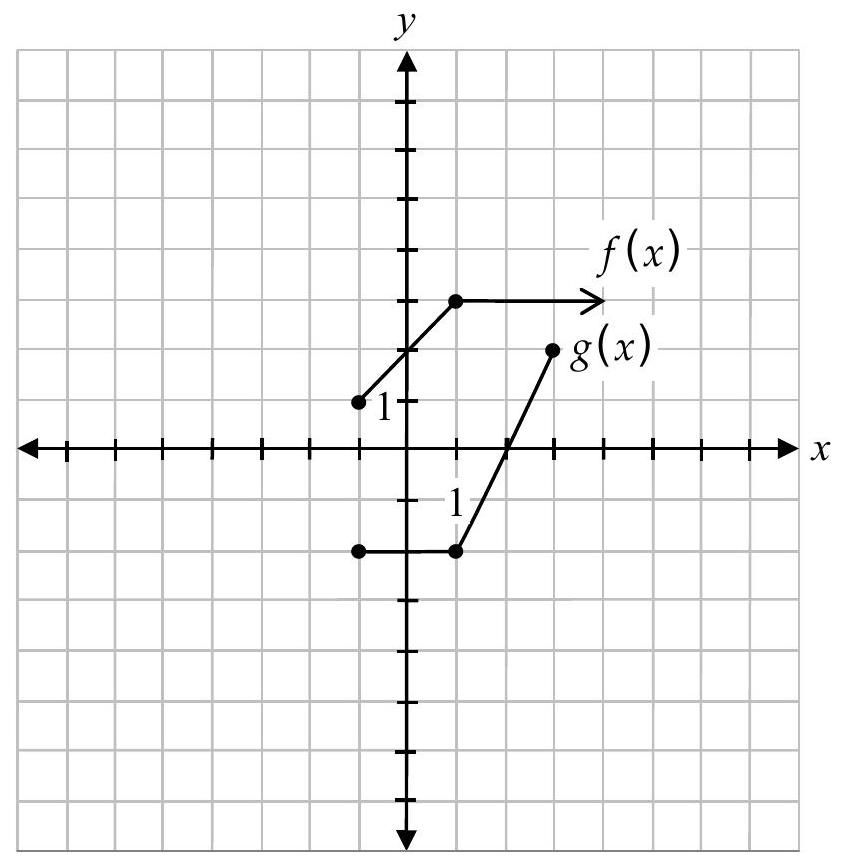
\includegraphics[max width=\textwidth, alt={}, center]{de5fb11a-28c7-4ac7-b7ff-0309cebac724-305_862_841_451_201}\\
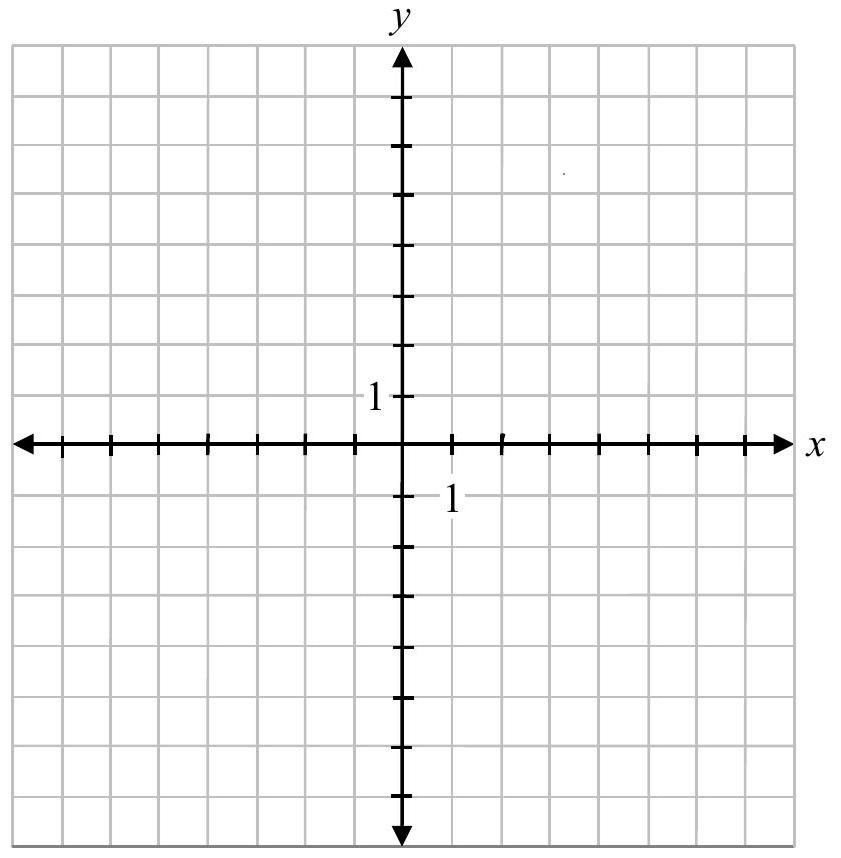
\includegraphics[max width=\textwidth, alt={}, center]{de5fb11a-28c7-4ac7-b7ff-0309cebac724-305_858_841_1392_623}

Identify the trigonometric function that is equivalent to $\sin \frac{\pi}{4} \cos \frac{\pi}{3}+\cos \frac{\pi}{4} \sin \frac{\pi}{3}$.\\
a) $\quad \sin \frac{2 \pi}{7}$\\
b) $\quad \sin \frac{7 \pi}{12}$\\
c) $\quad \cos \frac{2 \pi}{7}$\\
d) $\quad \cos \frac{7 \pi}{12}$

\section*{Question 20}
Identify the logarithmic form of $5^{x}=6$.\\
a) $\log _{5} x=6$\\
b) $\log _{5} 6=x$\\
c) $\log _{6} x=5$\\
d) $\log _{6} 5=x$

Given $f(\theta)=3 \cos 2 \theta-1$ and $g(\theta)=\sin \theta+1$, identify which statement is true.\\
a) Both functions have the same period.\\
b) Both functions have the same amplitude.\\
c) Both functions have the same minimum value.\\
d) Both functions have the same maximum value.

Identify the fourth term in the expansion of $(x+y)^{5}$.\\
a) $10 x^{4} y$\\
b) $10 x^{3} y^{2}$\\
c) $10 x^{2} y^{3}$\\
d) $10 x y^{4}$

Given the graphs of $f(x)$ and $g(x)$, identify the choice with all of the solutions of the equation $f(x)=g(x)$.\\
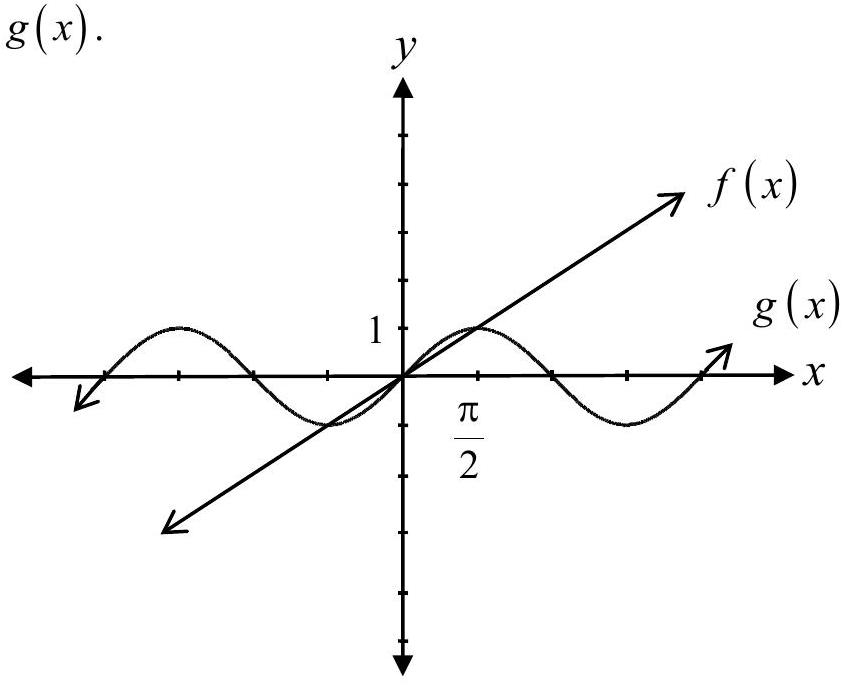
\includegraphics[max width=\textwidth, alt={}, center]{de5fb11a-28c7-4ac7-b7ff-0309cebac724-308_691_854_446_343}\\
a) $x=-2 \pi,-\pi, 0, \pi, 2 \pi$\\
b) $x=-\frac{\pi}{2}, 0, \frac{\pi}{2}$\\
c) $x=\frac{\pi}{2}$\\
d) $x=-1,0,1$

Identify the graph of $f^{-1}(x)$ if $f(x)=x^{2}-9, x \geq 0$.

\begin{figure}[h]
\begin{center}
\captionsetup{labelformat=empty}
\caption{a)}
  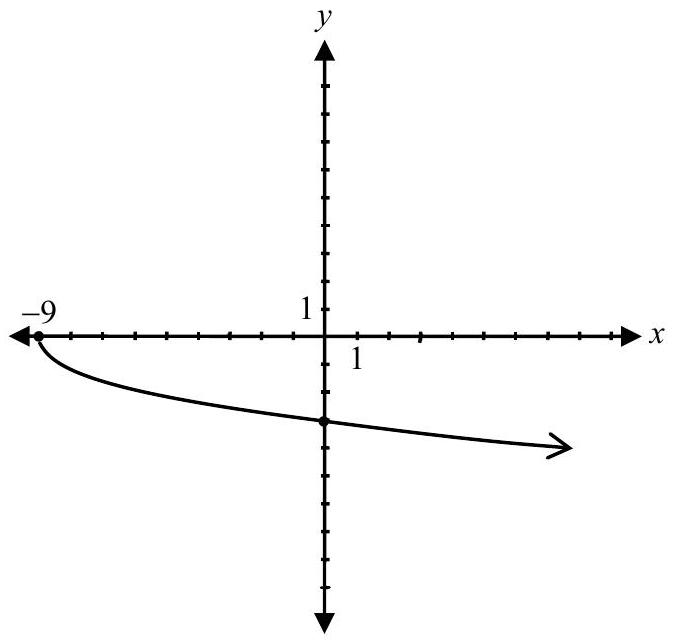
\includegraphics[alt={},max width=\textwidth]{de5fb11a-28c7-4ac7-b7ff-0309cebac724-309_644_677_519_292}
\end{center}
\end{figure}

\begin{figure}[h]
\begin{center}
\captionsetup{labelformat=empty}
\caption{b)}
  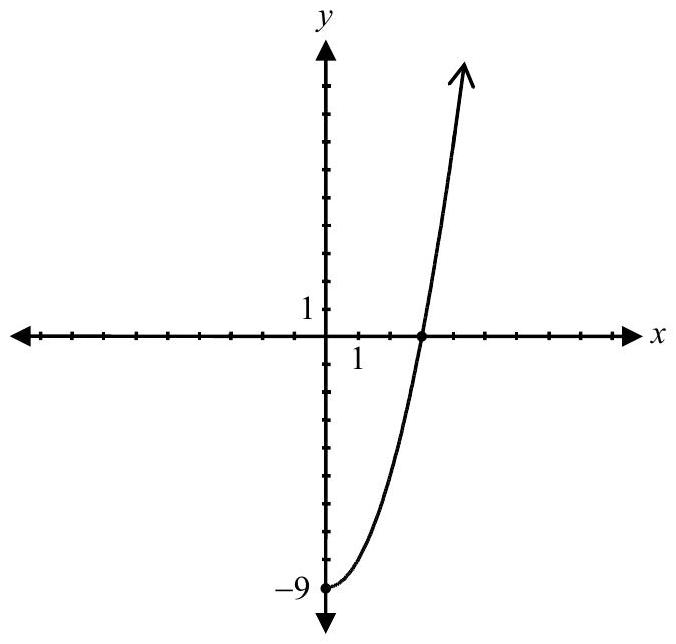
\includegraphics[alt={},max width=\textwidth]{de5fb11a-28c7-4ac7-b7ff-0309cebac724-309_644_676_519_1151}
\end{center}
\end{figure}

\begin{figure}[h]
\begin{center}
\captionsetup{labelformat=empty}
\caption{c)}
  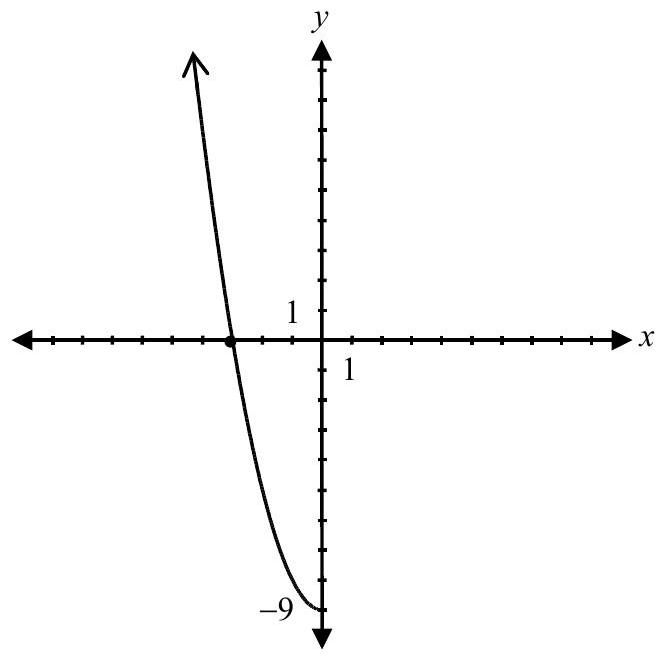
\includegraphics[alt={},max width=\textwidth]{de5fb11a-28c7-4ac7-b7ff-0309cebac724-309_656_665_1375_296}
\end{center}
\end{figure}

\begin{figure}[h]
\begin{center}
\captionsetup{labelformat=empty}
\caption{d)}
  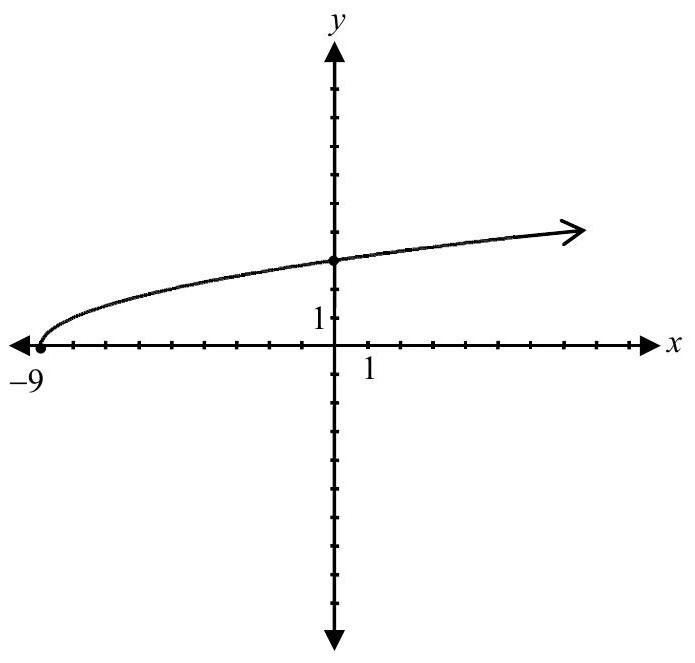
\includegraphics[alt={},max width=\textwidth]{de5fb11a-28c7-4ac7-b7ff-0309cebac724-309_663_695_1368_1151}
\end{center}
\end{figure}

Using the remainder theorem, identify which value of $x$ results in a remainder of zero given $p(x)=x^{3}+7 x^{2}+14 x+8$.\\
a) 1\\
b) 0\\
c) -1\\
d) -3

Evaluate $\cos \left(\cos \left(\frac{3 \pi}{2}\right)\right)$.\\
a) 1\\
b) $\frac{1}{2}$\\
c) 0\\
d) -1

Match the following equations with their graphs:

\section*{Place the appropriate letter in this column.}
$$
\begin{aligned}
& f(x)=(x-1)^{3}(x+1)(x-3) \\
& g(x)=(x+1)^{2}(x-1)(x+3) \\
& h(x)=-2(x-1)^{2}(x+1)(x-3) \\
& k(x)=2(x+1)^{2}(x-1)(x+3)
\end{aligned}
$$

\begin{figure}[h]
\begin{center}
\captionsetup{labelformat=empty}
\caption{A)}
  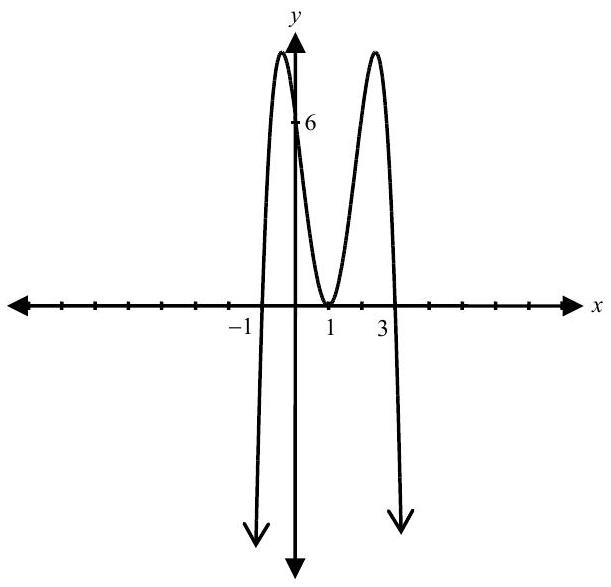
\includegraphics[alt={},max width=\textwidth]{de5fb11a-28c7-4ac7-b7ff-0309cebac724-311_587_611_1207_251}
\end{center}
\end{figure}

\begin{center}
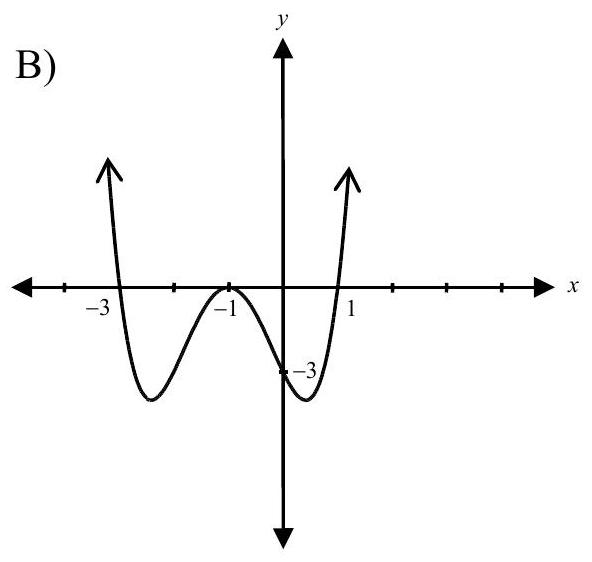
\includegraphics[max width=\textwidth, alt={}]{de5fb11a-28c7-4ac7-b7ff-0309cebac724-311_562_592_1228_1082}
\end{center}

\begin{figure}[h]
\begin{center}
\captionsetup{labelformat=empty}
\caption{C)}
  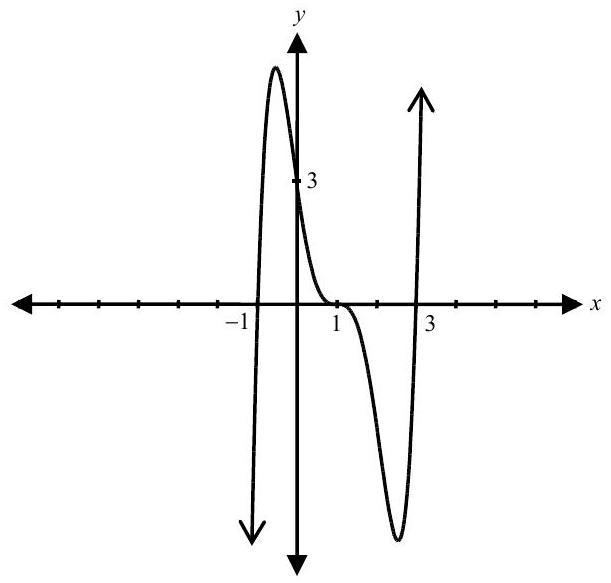
\includegraphics[alt={},max width=\textwidth]{de5fb11a-28c7-4ac7-b7ff-0309cebac724-311_583_611_1925_251}
\end{center}
\end{figure}

\begin{center}
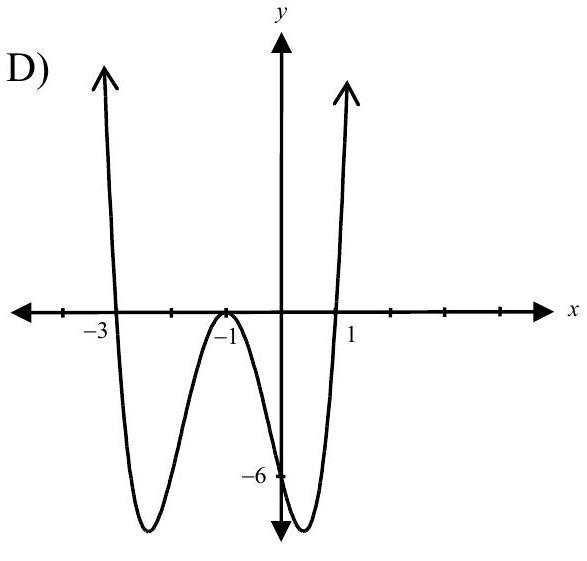
\includegraphics[max width=\textwidth, alt={}]{de5fb11a-28c7-4ac7-b7ff-0309cebac724-311_561_587_1912_1091}
\end{center}

If $\log 6=p, \log 5=r$ and $\log 2=q$, express $\log 60$ in terms of $p, q$ and $r$.

Sketch the graph of $y=\sqrt{-2 x}+1$.\\
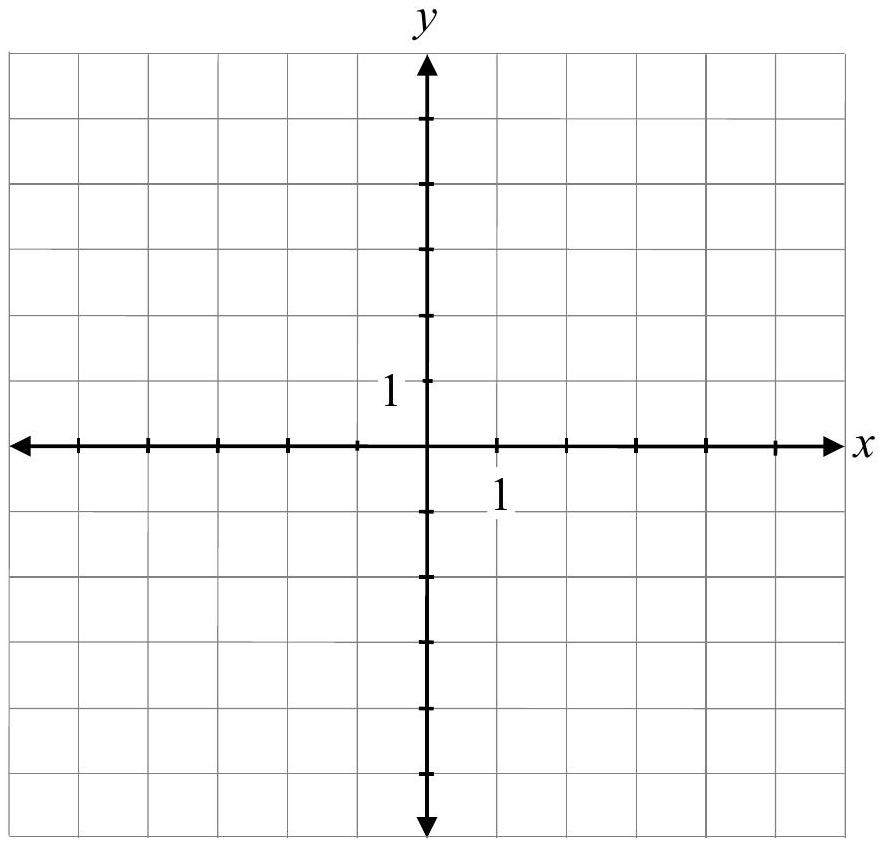
\includegraphics[max width=\textwidth, alt={}, center]{de5fb11a-28c7-4ac7-b7ff-0309cebac724-313_845_884_554_618}

Justify why the letters of the word FRANCE have a greater number of possible arrangements than the letters of the word CANADA.

\section*{Question 31}
a) 1 mark\\
b) 3 marks

Given $f(x)=\frac{1}{x-2}$ and $g(x)=x+5$,\\
a) determine the equation for $f(g(x))$.\\
$f(g(x))=$\\
b) sketch the graph of $f(g(x))$.\\
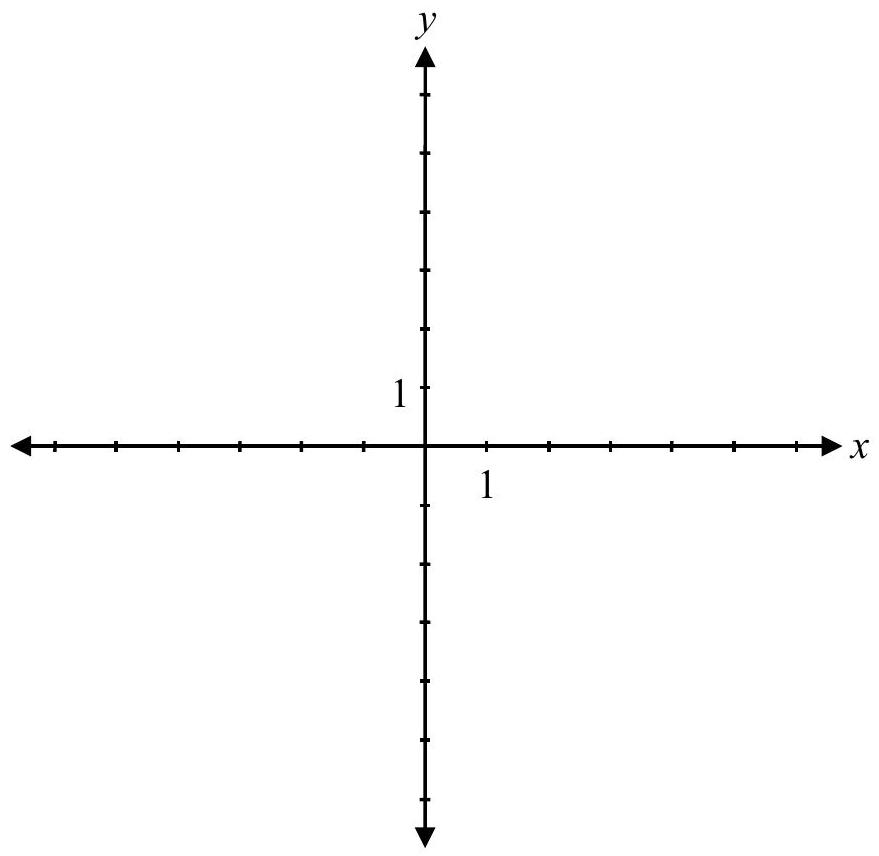
\includegraphics[max width=\textwidth, alt={}, center]{de5fb11a-28c7-4ac7-b7ff-0309cebac724-315_856_879_1555_277}

\section*{Question 32}
a) 3 marks\\
b) 1 mark127\\
128

Given that $\sin \alpha=\frac{3}{7}$, where $\alpha$ is in Quadrant II, and $\cos \beta=\frac{4}{5}$, where $\beta$ is in Quadrant IV, determine the exact value of:\\
a) $\sin (\alpha-\beta)$\\
b) $\cos 2 \alpha$

Determine the domain and range of $f(x)=\sqrt{x-5}-1$.

Domain: $\_\_\_\_$

Range: $\_\_\_\_$

Justify why 4.7 is a better estimate than 4.3 for the value of $\log _{2} 26$.

Sketch the graph of the function:

$$
f(x)=\frac{x(x-2)(x-4)}{(x-2)}
$$

\begin{center}
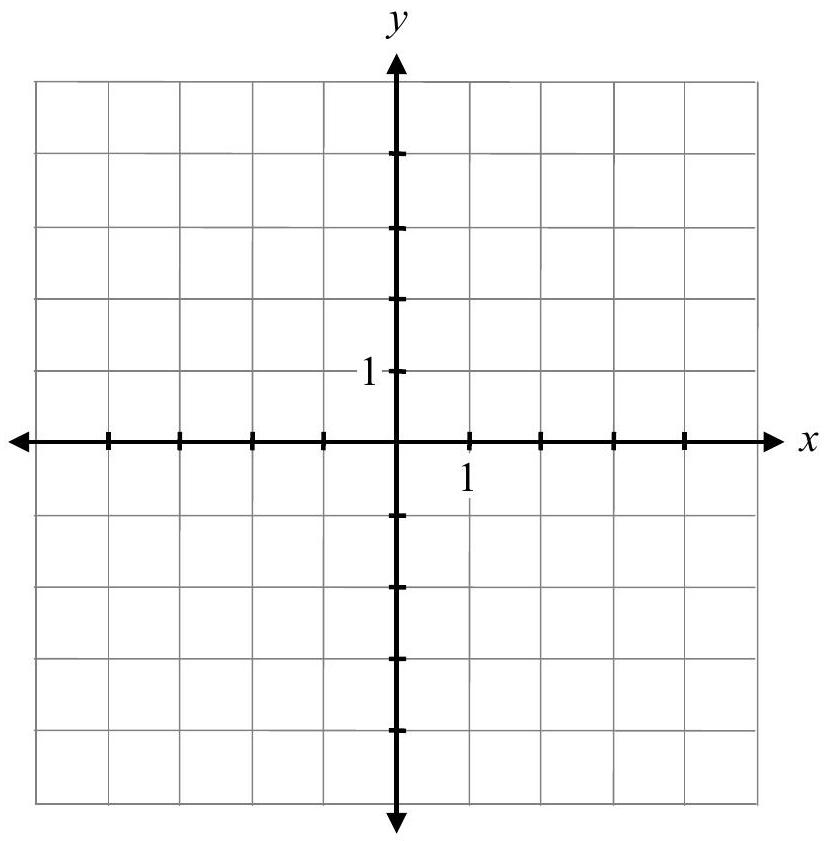
\includegraphics[max width=\textwidth, alt={}]{de5fb11a-28c7-4ac7-b7ff-0309cebac724-319_841_826_623_620}
\end{center}

Evaluate:

$$
\sec ^{2}\left(\frac{\pi}{6}\right)+\tan \left(\frac{7 \pi}{6}\right) \csc \left(-\frac{2 \pi}{3}\right)
$$

The graph of $f(x)=3 x+7$ is reflected over the $y$-axis.\\
Determine the equation of the new function.

$$
y=
$$

Determine the equations of all of the asymptotes of the function:

$$
y=\frac{2 x+1}{x-3}
$$

One of the zeros of $p(x)=x^{3}+6 x^{2}-32$ is $x=2$. Determine all of the other zeros of $p(x)$.

Sketch the graph of $y=-2^{x}+2$.\\
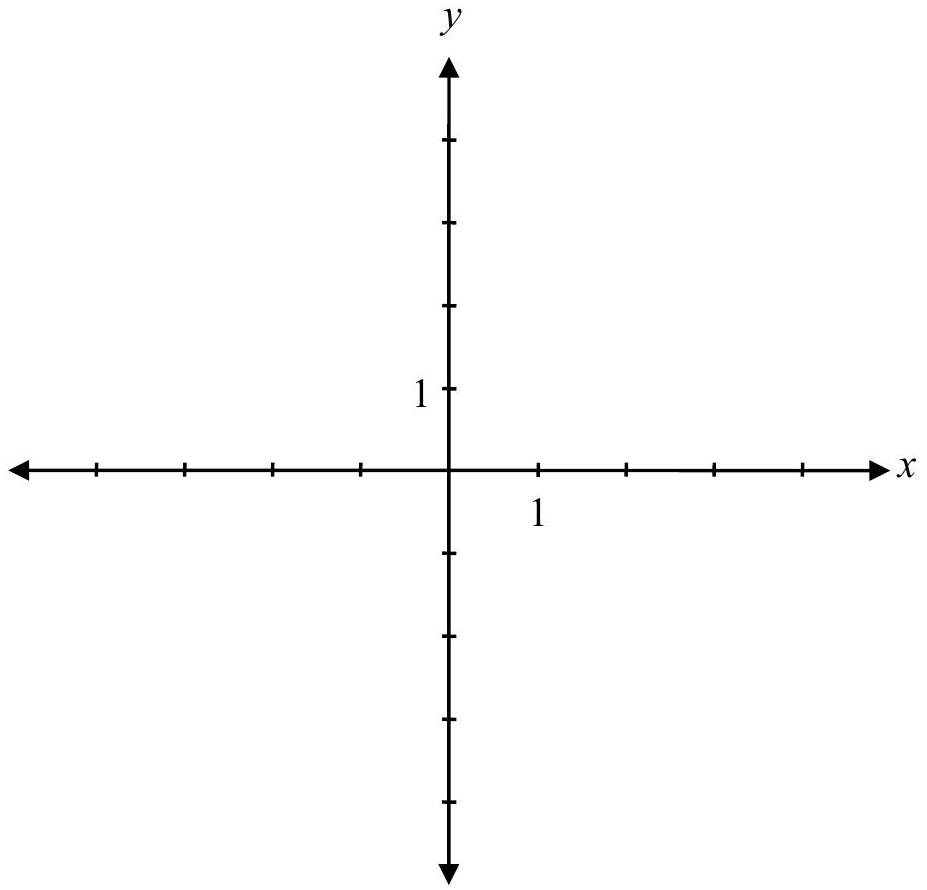
\includegraphics[max width=\textwidth, alt={}, center]{de5fb11a-28c7-4ac7-b7ff-0309cebac724-323_890_927_610_451}

Given the function $f(x)=\frac{2}{x}-1$, justify why $f(f(2))$ is undefined.

The following graph represents the volume of air in an adult's lungs. If $V(t)$ is the volume of air in litres and $t$ is the time in seconds, determine an equation that represents this sinusoidal function.\\
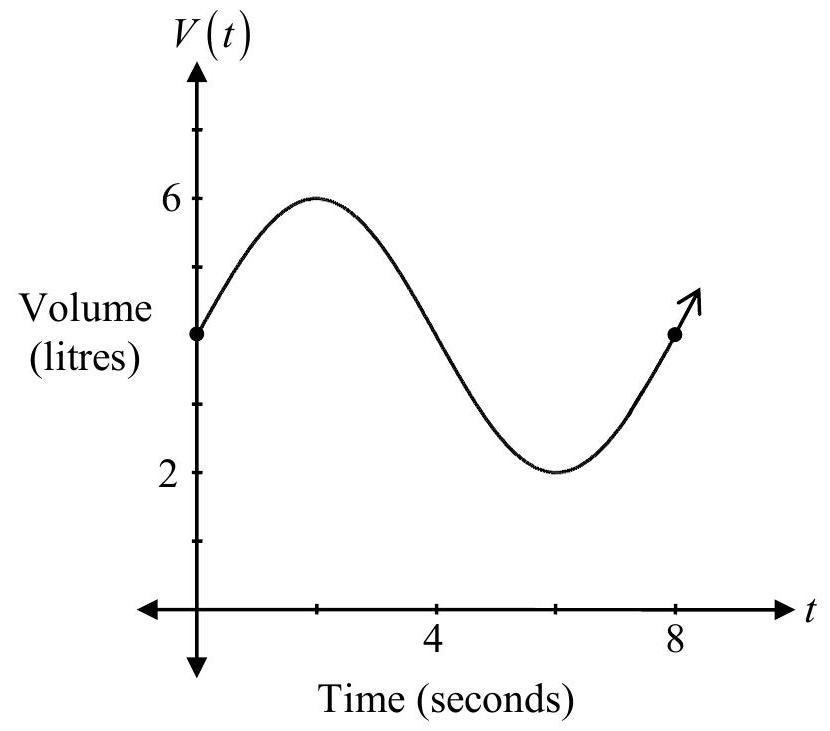
\includegraphics[max width=\textwidth, alt={}, center]{de5fb11a-28c7-4ac7-b7ff-0309cebac724-325_731_830_552_210}\\
$V(t)=$ $\_\_\_\_$

Explain why the domain of $y=\log _{2}(x-1)$ is $x>1$.

The point ( $-2,7$ ) is on the terminal arm of an angle in standard position.\\
Determine the coordinates of the corresponding point, $P(\theta)$, on the unit circle.

Sketch a graph of $P(x)$ that satisfies all of the following conditions:

\begin{itemize}
  \item $P(x)$ is a polynomial function of degree 3 .
  \item $P(x)$ has a zero at -3 with a multiplicity of 2 .
  \item $P(x)$ has a zero at 1 .
  \item $P(x)$ has a leading coefficient of -3 .\\
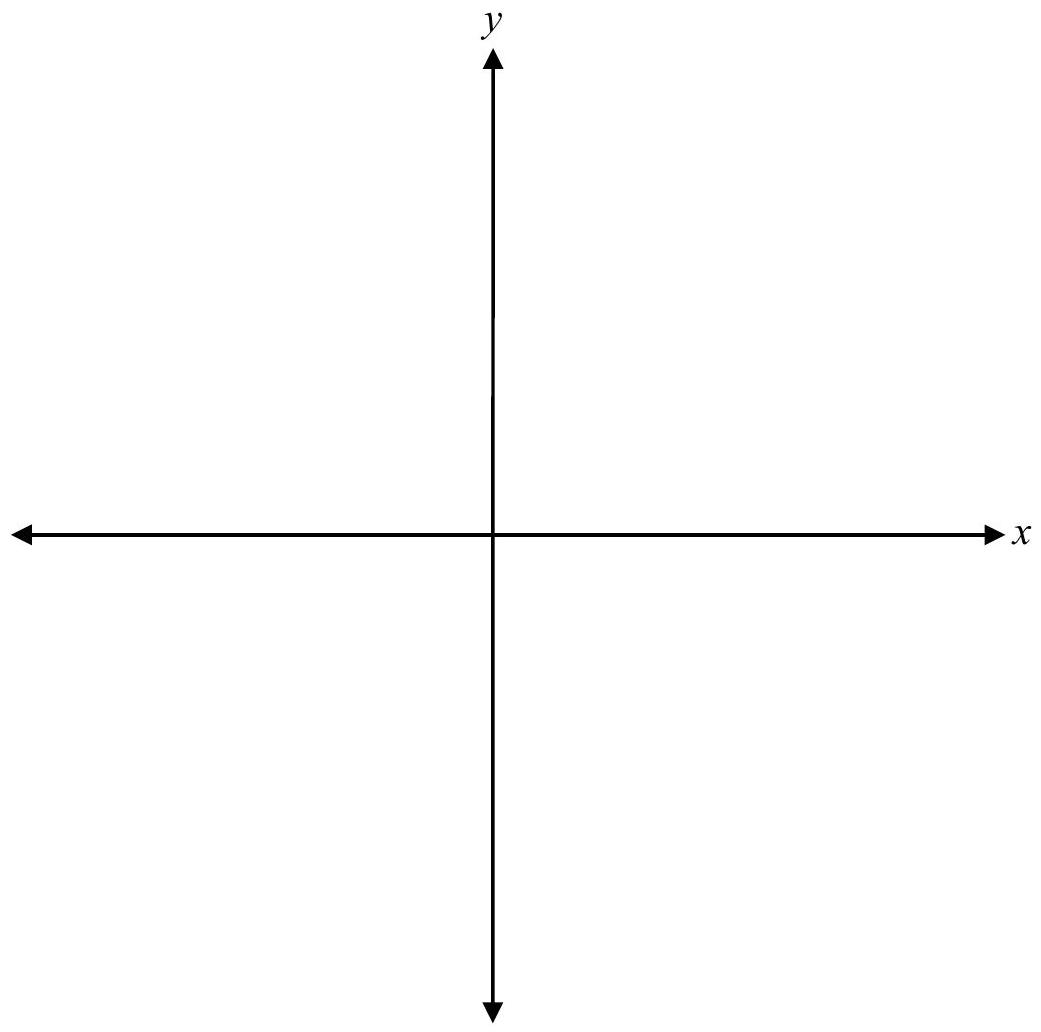
\includegraphics[max width=\textwidth, alt={}, center]{de5fb11a-28c7-4ac7-b7ff-0309cebac724-328_1032_1041_870_543}
\end{itemize}

Determine how many 4 -digit numbers greater than 4000 can be made using the digits $2,3,4,5$, and 6 if repetitions are not allowed.

A section of a car windshield is cleaned by a wiper as shown in the diagram below. The arm of the wiper is 22 inches, and it rotates through a central angle of $132^{\circ}$. Determine the length of the arc that is created by the tip of the wiper.\\
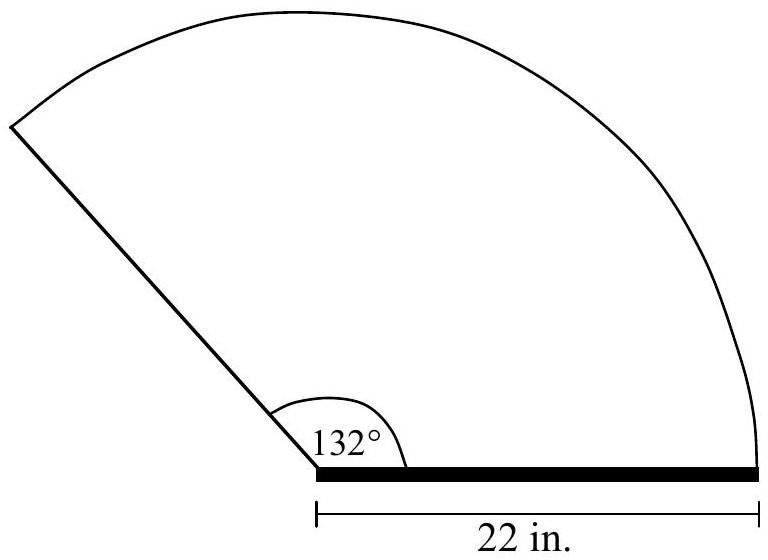
\includegraphics[max width=\textwidth, alt={}, center]{de5fb11a-28c7-4ac7-b7ff-0309cebac724-330_560_768_586_678}

There are 20 boys and 11 girls who can be selected to be on a team.\\
Determine the number of ways that 7 boys and 5 girls can be selected for this team.

A water filtration system which removes impurities from a sample of water can be modelled by $P=0.25(0.55)^{n}$, where:\\
$P=$ the percentage of impurities remaining, in decimal form\\
$n=$ the number of filters\\
Determine, algebraically, how many filters are required so that less than $1 \%$ of the impurities remain in the water sample. Express your answer as a whole number.

In the binomial expansion of $\left(x^{2}-\frac{2}{y}\right)^{8}$, determine the middle term in simplified form.

Solve the following equation algebraically over the interval $[0,2 \pi]$.

$$
6 \sin ^{2} \theta+\sin \theta-1=0
$$

Given the graph of $y=f(x)$, sketch the graph of $y=f(-x+4)$.\\
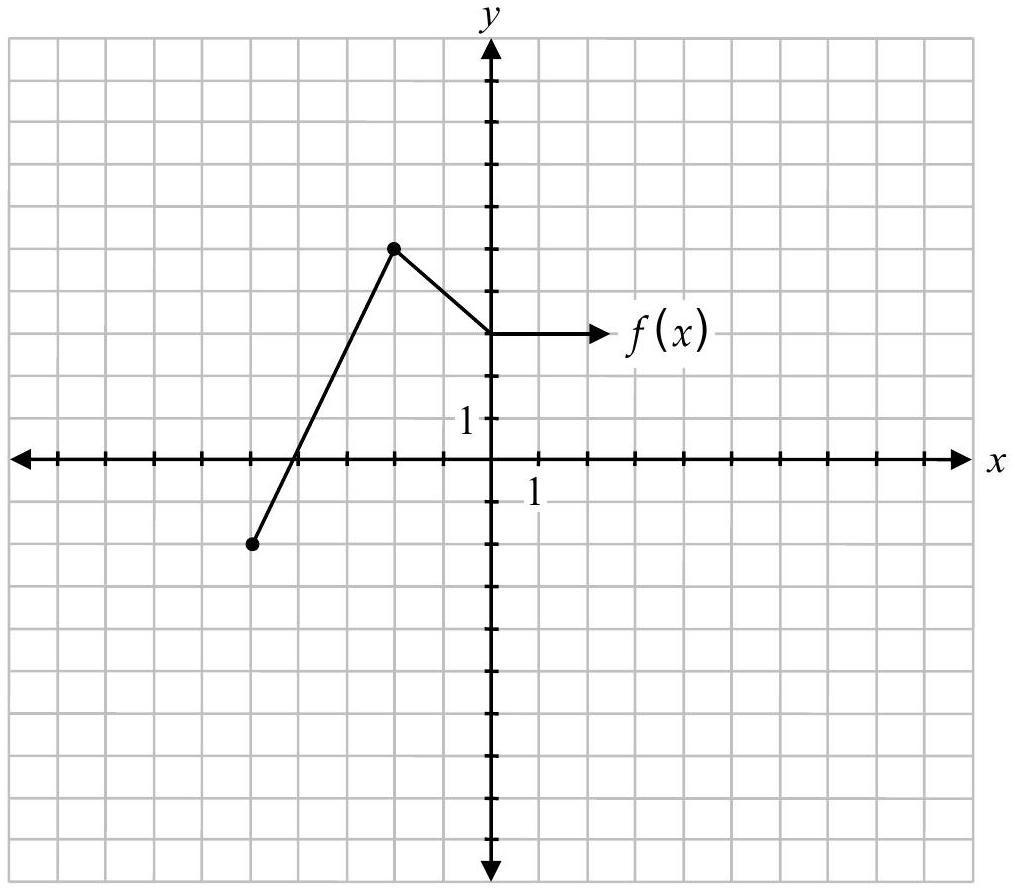
\includegraphics[max width=\textwidth, alt={}, center]{de5fb11a-28c7-4ac7-b7ff-0309cebac724-335_890_1015_466_468}\\
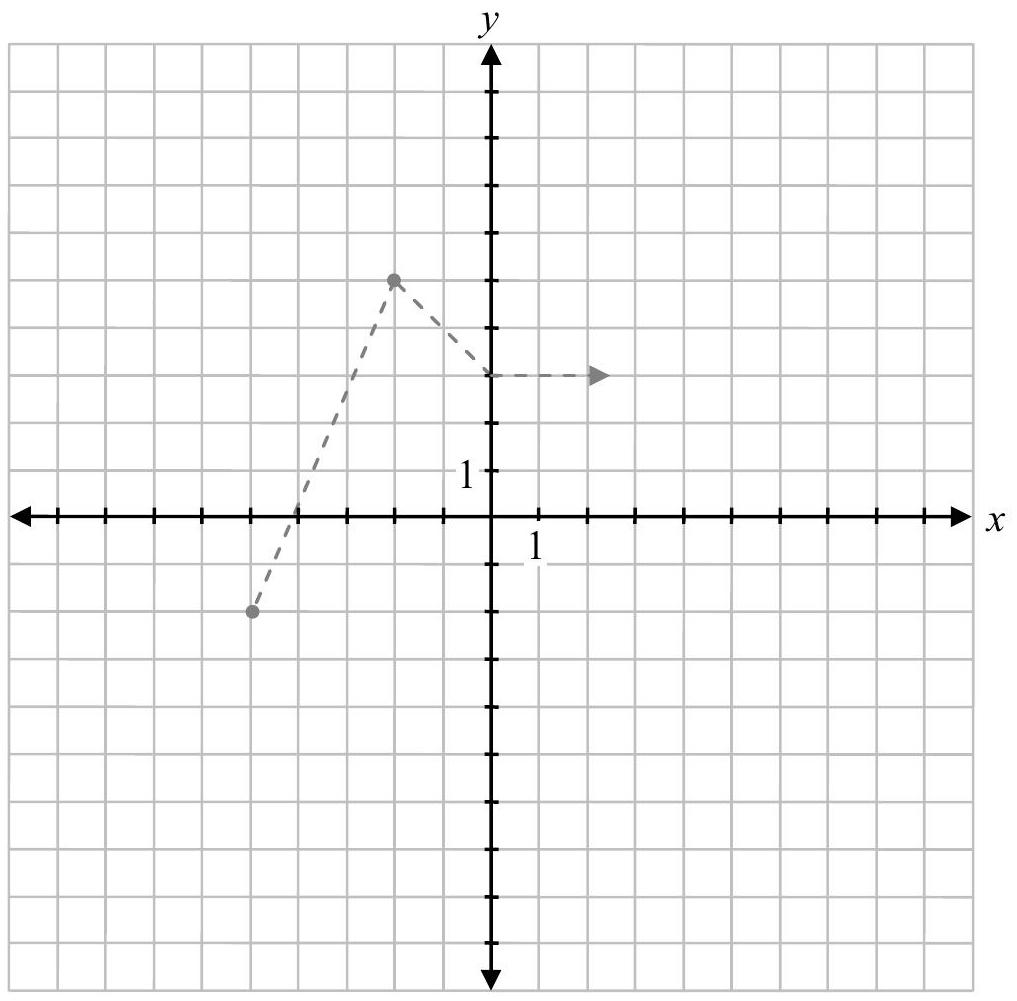
\includegraphics[max width=\textwidth, alt={}, center]{de5fb11a-28c7-4ac7-b7ff-0309cebac724-335_1001_1017_1533_468}

The graph of $f(x)$ has already been drawn for your reference.\\
No marks will be awarded for the graph of $f(x)$.

Given the following triangle, determine $\csc \theta$.\\
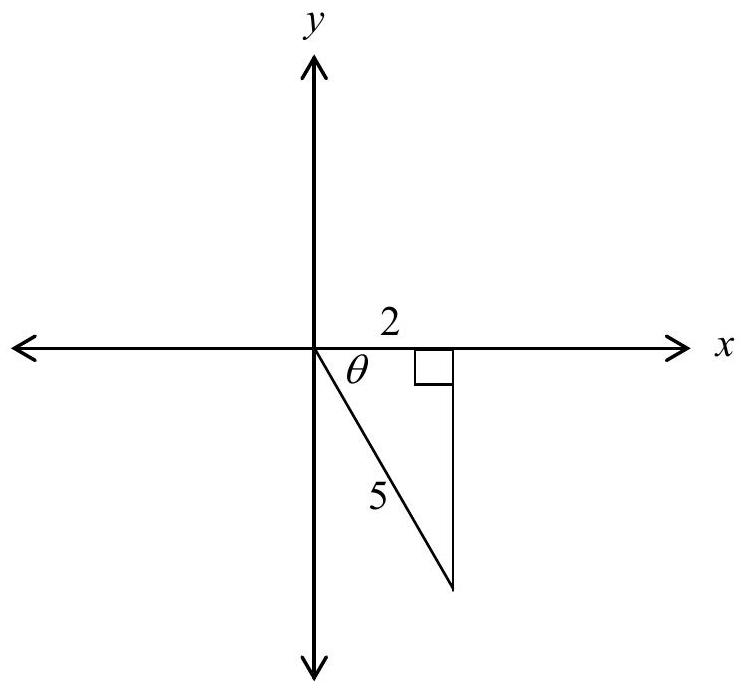
\includegraphics[max width=\textwidth, alt={}, center]{de5fb11a-28c7-4ac7-b7ff-0309cebac724-336_691_747_526_674}

Solve algebraically.

$$
{ }_{n} P_{2}=9 n
$$

Describe the transformations applied to the graph of $f(x)$ to obtain the graph of $g(x)$.\\
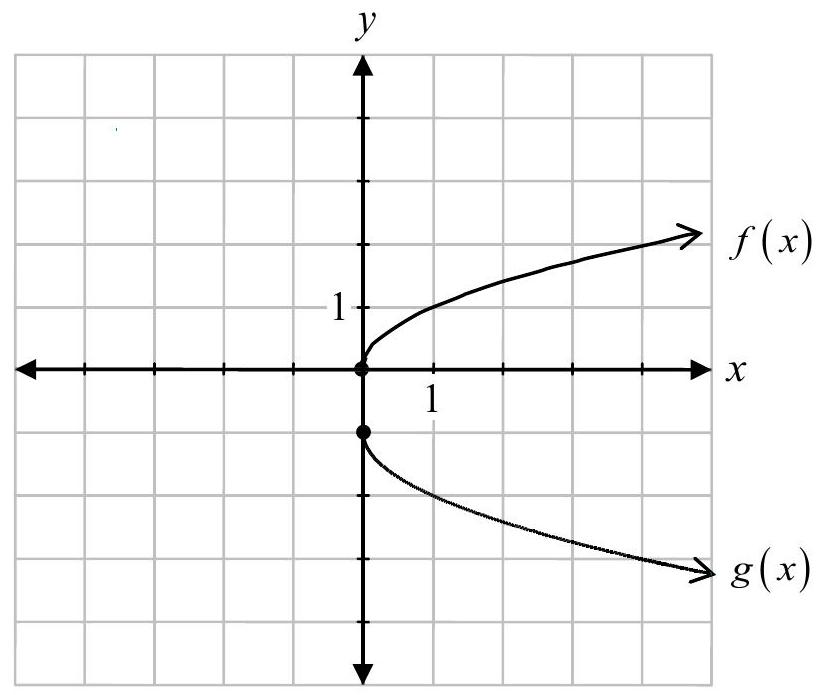
\includegraphics[max width=\textwidth, alt={}, center]{de5fb11a-28c7-4ac7-b7ff-0309cebac724-338_695_824_524_627}

Determine, algebraically, the value of the leading coefficient of the graph of the polynomial function, $p(x)$.\\
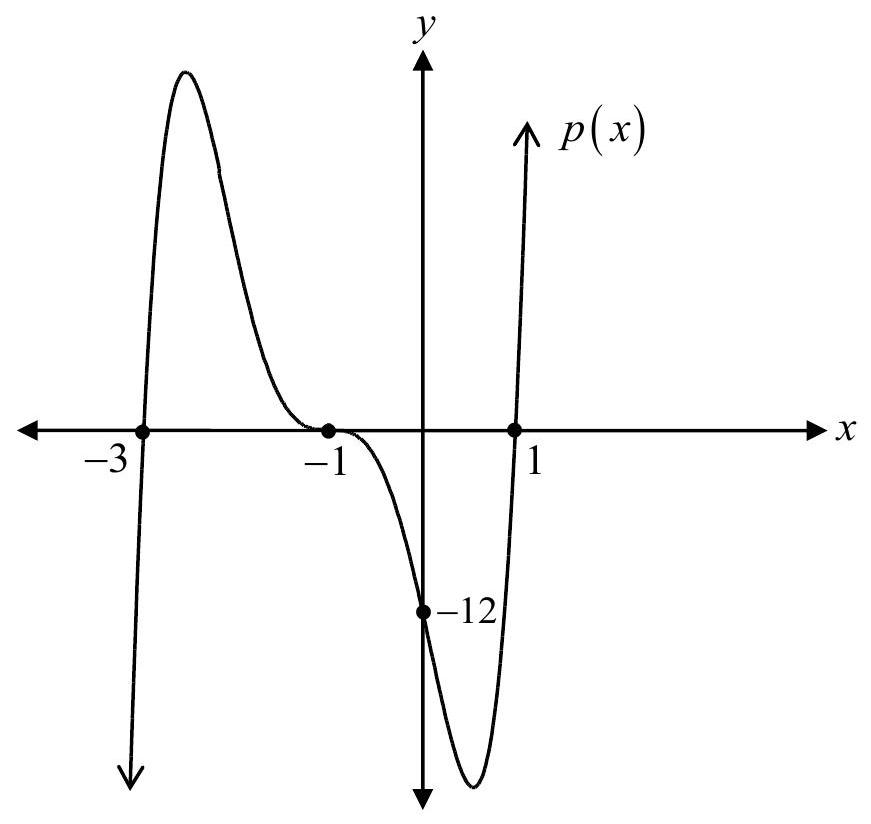
\includegraphics[max width=\textwidth, alt={}, center]{de5fb11a-28c7-4ac7-b7ff-0309cebac724-339_824_871_489_560}

Frank, Liam, Chan, and Thao are going to a movie.\\
Determine the number of ways they can sit in a row of four chairs, if Frank and Chan must sit beside each other.

Determine, algebraically, if $f(x)=\frac{1}{x+5}$ and $g(x)=\frac{1}{x-5}$ are inverses of each other.\\
Justify your answer.

Using the graphs of $y=f(x)$ and $y=g(x)$, solve $f(x)=g(x)$.\\
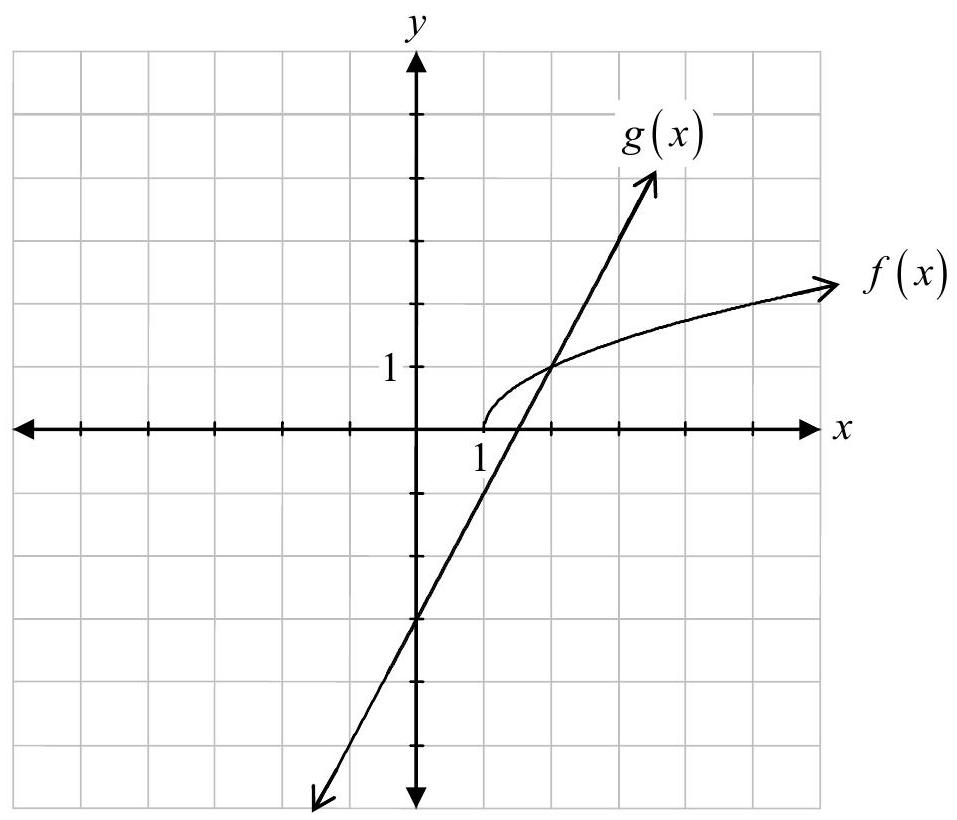
\includegraphics[max width=\textwidth, alt={}, center]{de5fb11a-28c7-4ac7-b7ff-0309cebac724-342_820_957_545_571}

An angle in standard position measures $\frac{3 \pi}{4}$.\\
Determine in which quadrant the terminal arm of this angle is located after a rotation of 3 radians.\\
Justify your answer.

Prove the following identity for all permissible values of $\theta$.

$$
\frac{\sin 2 \theta}{1-\cos 2 \theta}=\cot \theta
$$

\begin{center}
\begin{tabular}{|l|l|}
\hline
Left-Hand Side & Right-Hand Side \\
\hline
\end{tabular}
\end{center}

If the range of $y=f(x)$ is $-3 \leq y \leq 6$, determine the range of $y=2 f(3 x)$.

Maurice incorrectly solved the equation, $\sin \theta+1=0$, over the interval $\left[0^{\circ}, 360^{\circ}\right]$.

$$
\begin{aligned}
& \sin \theta+1=0 \\
& \sin \theta=-1 \\
& \sin \theta=270^{\circ}
\end{aligned}
$$

Describe his error.

If $P(3,5)$ is a point on the graph of $y=f(x)$, identify the corresponding point on the graph of $y=f(x-1)+7$.\\
a) $(2,12)$\\
b) $(4,-2)$\\
c) $(2,-2)$\\
d) $(4,12)$

Question 19

Identify how the graph of $y=3^{x}$ is transformed to the graph of $y=3^{-x}$.\\
a) reflected over the $x$-axis\\
b) reflected over the $y$-axis\\
c) reflected over both the $x$-axis and the $y$-axis\\
d) reflected over the line $y=x$

Question 20

Identify the equation $\log _{a} b=c$ in exponential form.\\
a) $b^{c}=a$\\
b) $a^{c}=b$\\
c) $a^{b}=c$\\
d) $c^{a}=b$

Identify the graph of $y=\tan x$.

\begin{figure}[h]
\begin{center}
\captionsetup{labelformat=empty}
\caption{a)}
  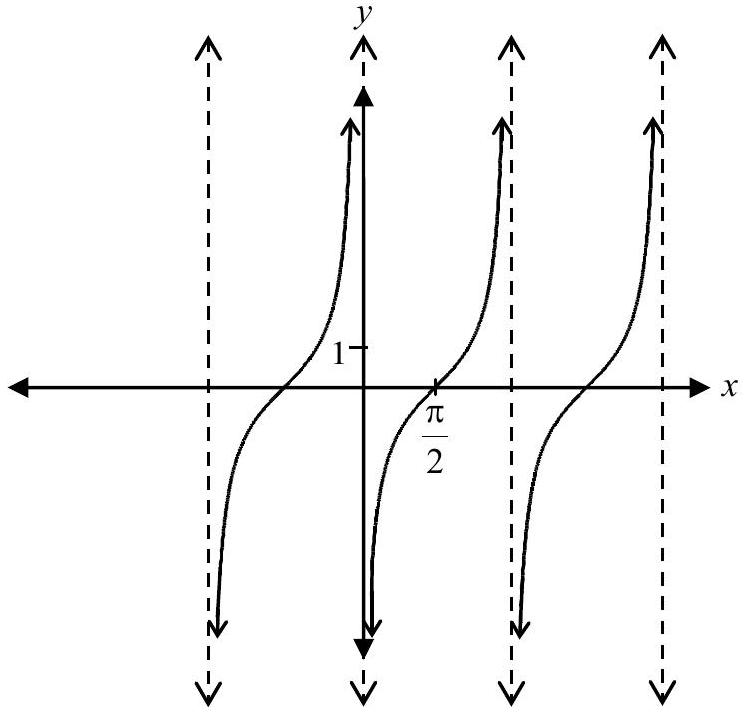
\includegraphics[alt={},max width=\textwidth]{de5fb11a-28c7-4ac7-b7ff-0309cebac724-347_715_747_517_257}
\end{center}
\end{figure}

\begin{figure}[h]
\begin{center}
\captionsetup{labelformat=empty}
\caption{b)}
  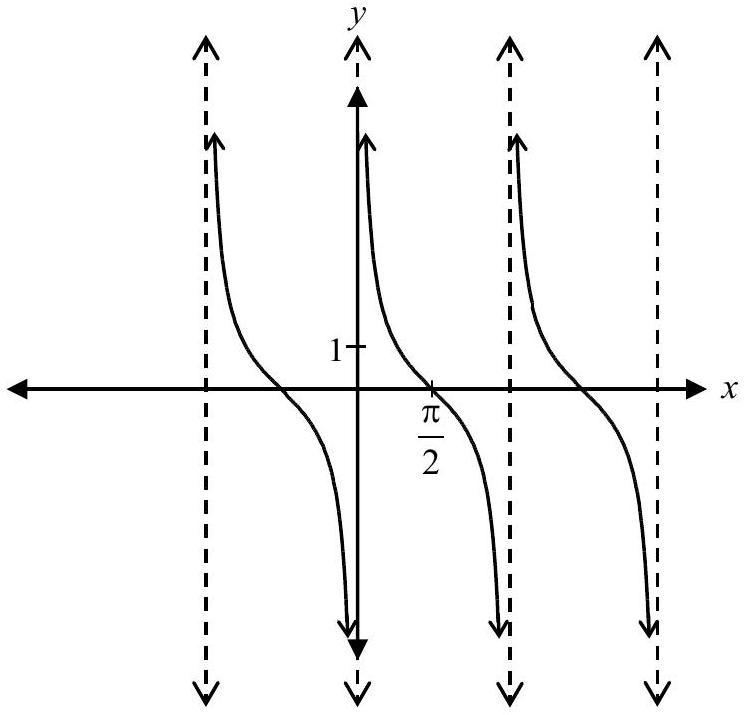
\includegraphics[alt={},max width=\textwidth]{de5fb11a-28c7-4ac7-b7ff-0309cebac724-347_715_746_517_1130}
\end{center}
\end{figure}

\begin{figure}[h]
\begin{center}
\captionsetup{labelformat=empty}
\caption{c)}
  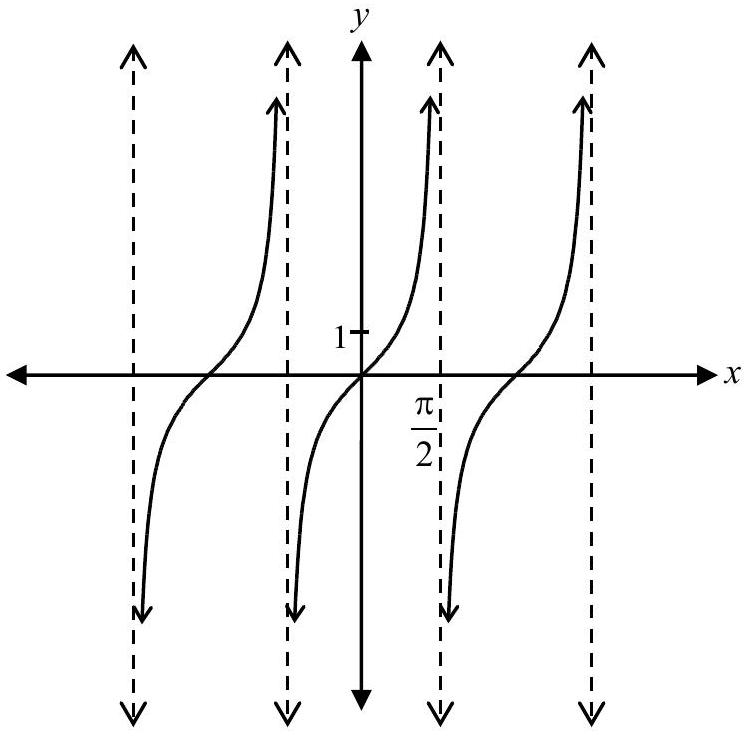
\includegraphics[alt={},max width=\textwidth]{de5fb11a-28c7-4ac7-b7ff-0309cebac724-347_736_746_1589_249}
\end{center}
\end{figure}

\begin{figure}[h]
\begin{center}
\captionsetup{labelformat=empty}
\caption{d)}
  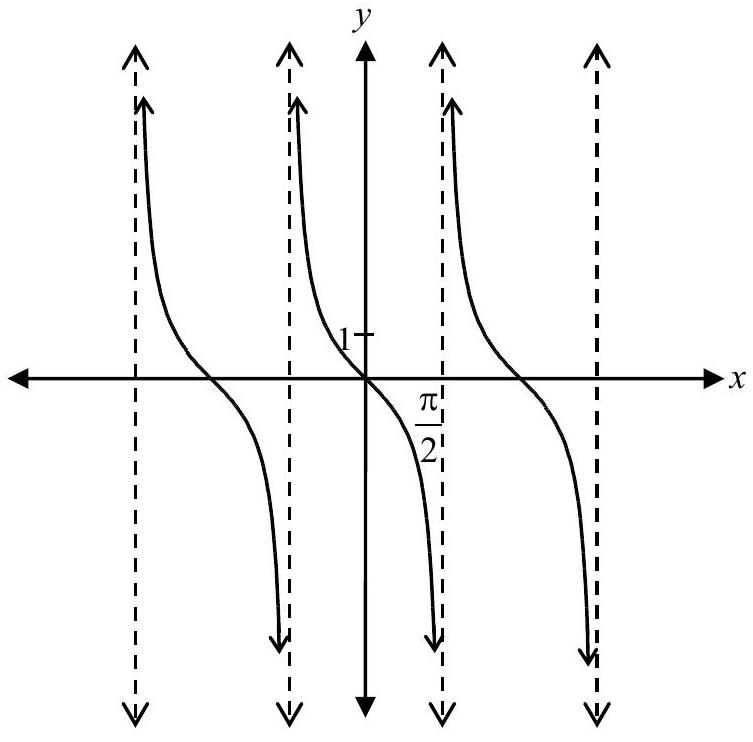
\includegraphics[alt={},max width=\textwidth]{de5fb11a-28c7-4ac7-b7ff-0309cebac724-347_742_753_1581_1125}
\end{center}
\end{figure}

Identify which of the following graphs represents a logarithmic function.

\begin{figure}[h]
\begin{center}
\captionsetup{labelformat=empty}
\caption{a)}
  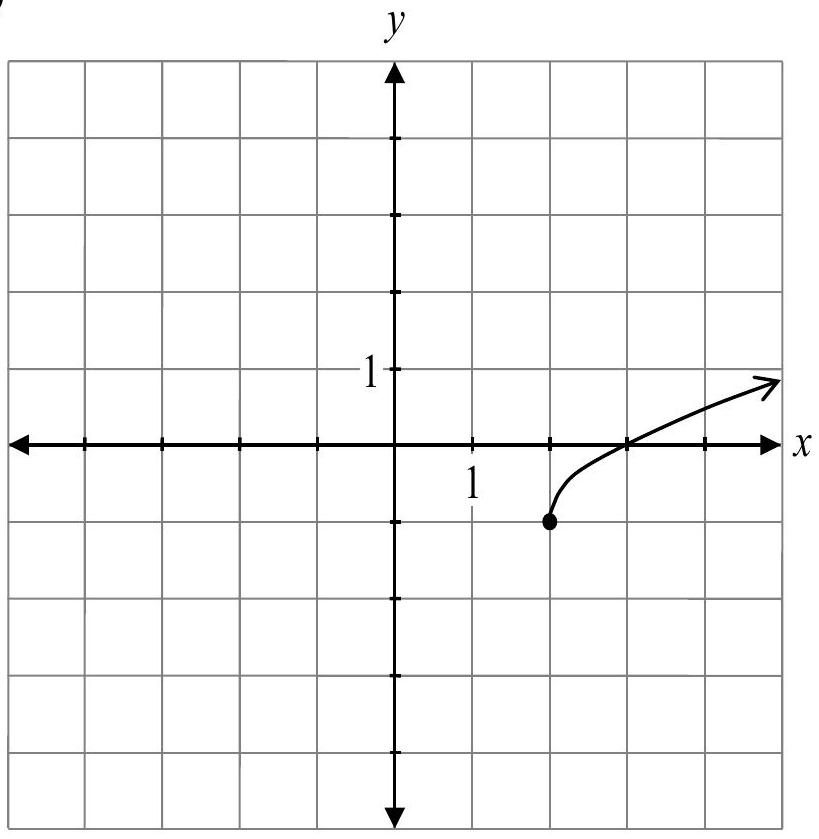
\includegraphics[alt={},max width=\textwidth]{de5fb11a-28c7-4ac7-b7ff-0309cebac724-348_839_819_582_236}
\end{center}
\end{figure}

\begin{figure}[h]
\begin{center}
\captionsetup{labelformat=empty}
\caption{b)}
  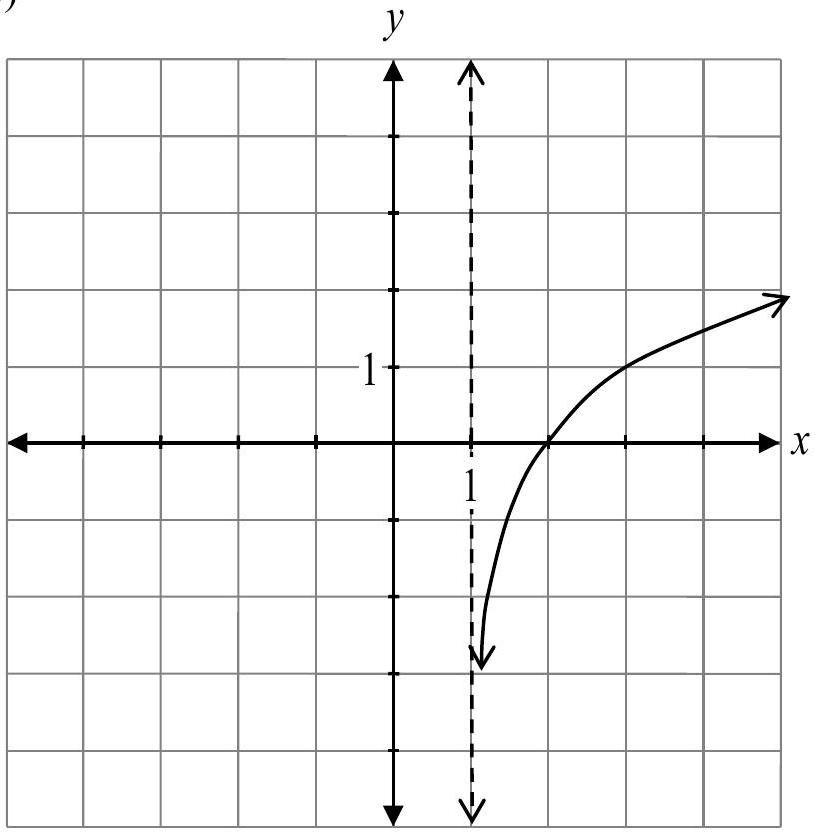
\includegraphics[alt={},max width=\textwidth]{de5fb11a-28c7-4ac7-b7ff-0309cebac724-348_834_820_584_1097}
\end{center}
\end{figure}

\begin{figure}[h]
\begin{center}
\captionsetup{labelformat=empty}
\caption{c)}
  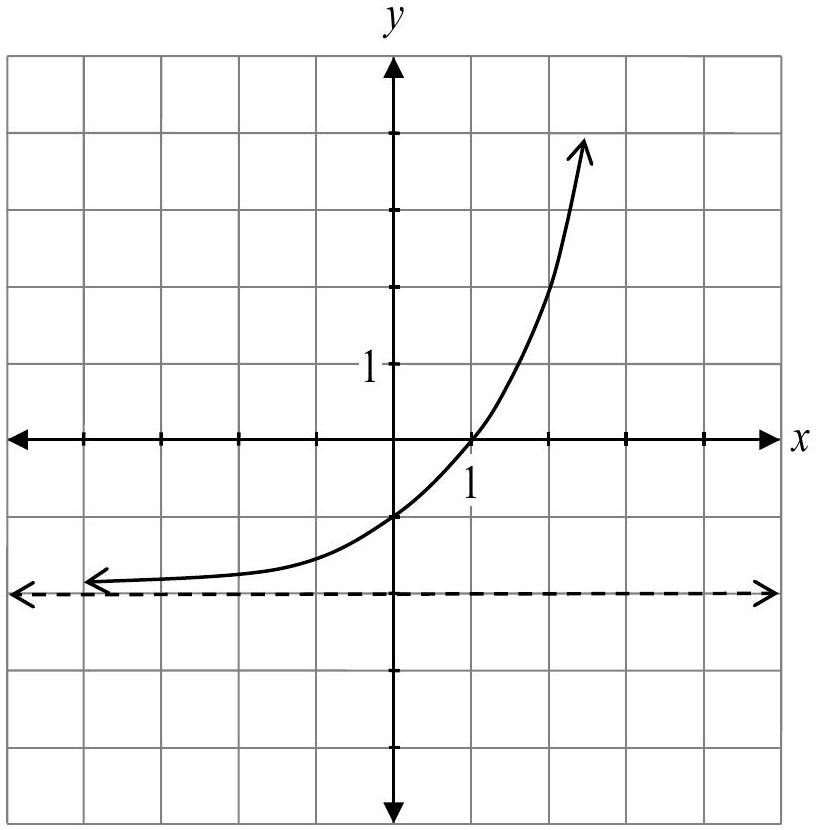
\includegraphics[alt={},max width=\textwidth]{de5fb11a-28c7-4ac7-b7ff-0309cebac724-348_830_817_1587_236}
\end{center}
\end{figure}

\begin{figure}[h]
\begin{center}
\captionsetup{labelformat=empty}
\caption{d)}
  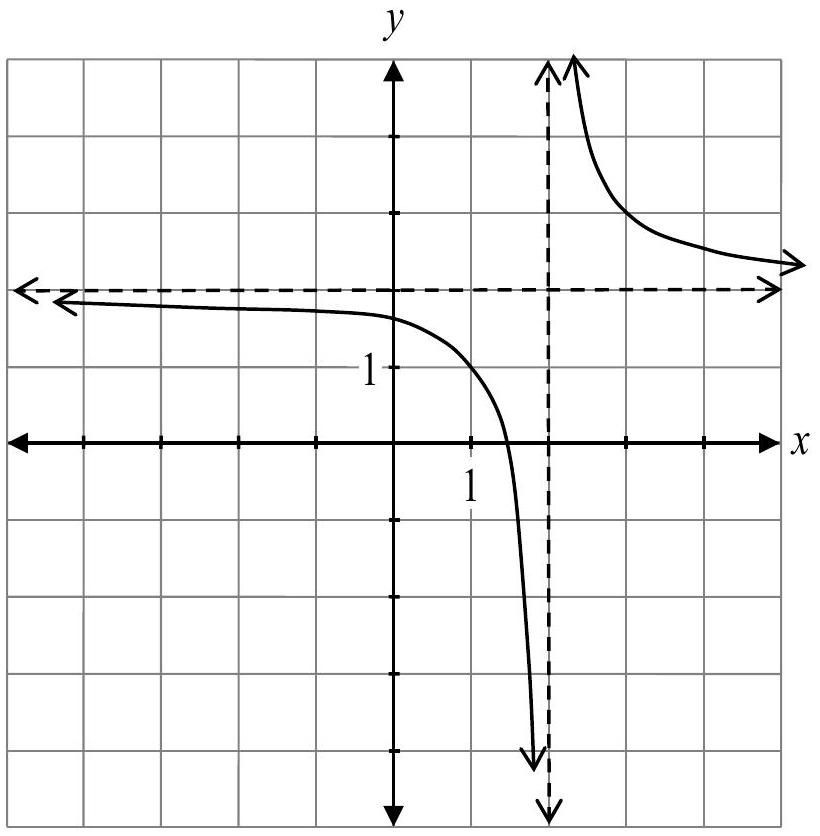
\includegraphics[alt={},max width=\textwidth]{de5fb11a-28c7-4ac7-b7ff-0309cebac724-348_836_820_1609_1108}
\end{center}
\end{figure}

If the volume of a box is represented by $V(x)=(x+4)(x+2)(x-1)$, identify a possible value of $x$.\\
a) -4\\
b) -1\\
c) 1\\
d) 4

Question 24

Identify a coterminal angle for $\theta=-\frac{\pi}{3}$.\\
a) $\frac{\pi}{3}$\\
b) $\frac{4 \pi}{3}$\\
c) $\frac{7 \pi}{3}$\\
d) $\frac{11 \pi}{3}$

Question 25

Identify the value of $n$ in the equation ${ }_{n} C_{3}={ }_{n} C_{6}$.\\
a) 3\\
b) 6\\
c) 9\\
d) 18

Identify the equation of the function, $f(x)$, for the following graph.\\
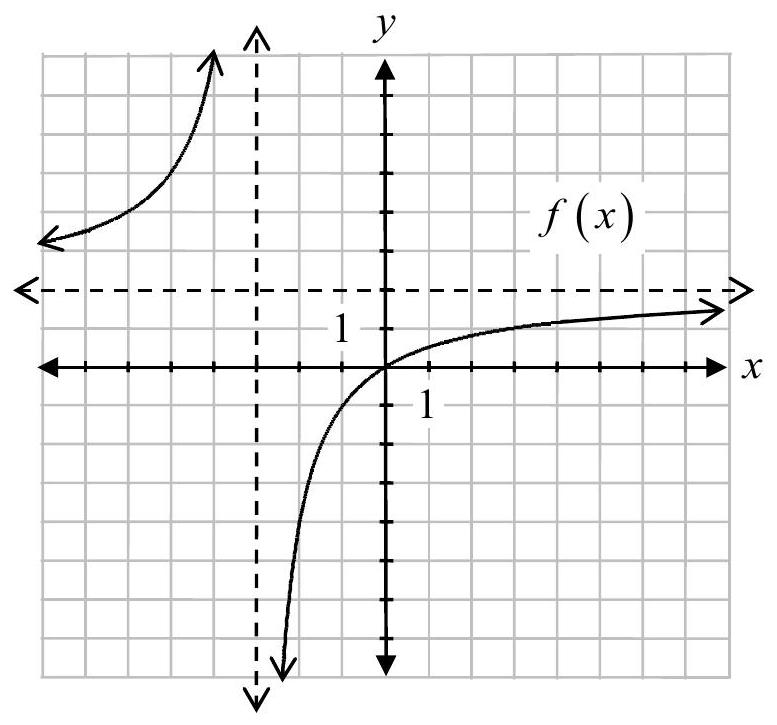
\includegraphics[max width=\textwidth, alt={}, center]{de5fb11a-28c7-4ac7-b7ff-0309cebac724-350_725_777_455_300}\\
a) $f(x)=\frac{2 x}{x+3}$\\
b) $f(x)=\frac{2}{x+3}$\\
c) $f(x)=\frac{2 x^{2}}{x(x+3)}$\\
d) $f(x)=\frac{3 x^{2}}{x(x+2)}$

Match the following radical functions with their graphs.\\
Place the appropriate letter in this column.

$$
\begin{aligned}
& f(x)=2 \sqrt{-(x+3)} \\
& g(x)=-2 \sqrt{(x+3)} \\
& h(x)=3 \sqrt{(x-2)} \\
& k(x)=\sqrt{3(x-2)}
\end{aligned}
$$

\begin{figure}[h]
\begin{center}
\captionsetup{labelformat=empty}
\caption{A)}
  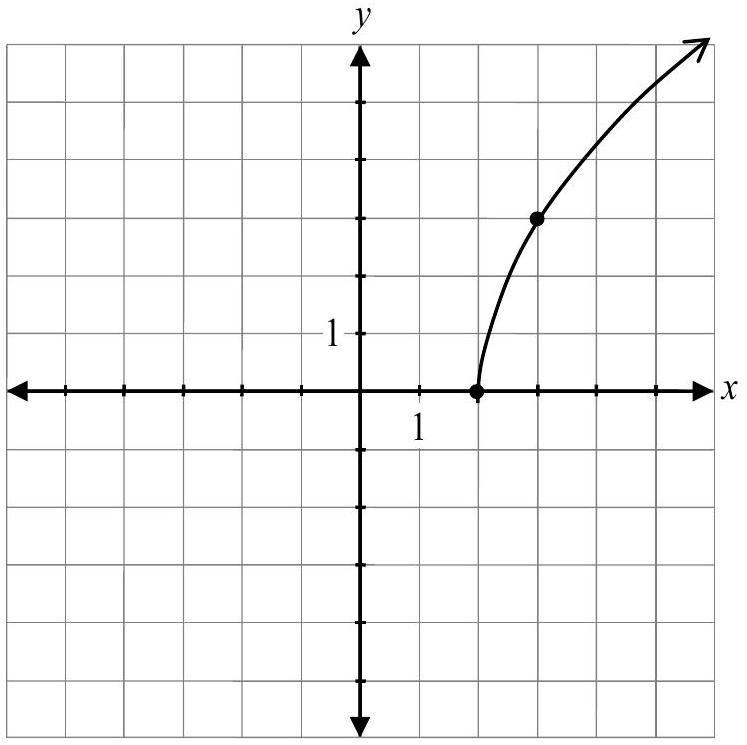
\includegraphics[alt={},max width=\textwidth]{de5fb11a-28c7-4ac7-b7ff-0309cebac724-351_745_747_1069_257}
\end{center}
\end{figure}

\begin{figure}[h]
\begin{center}
\captionsetup{labelformat=empty}
\caption{B)}
  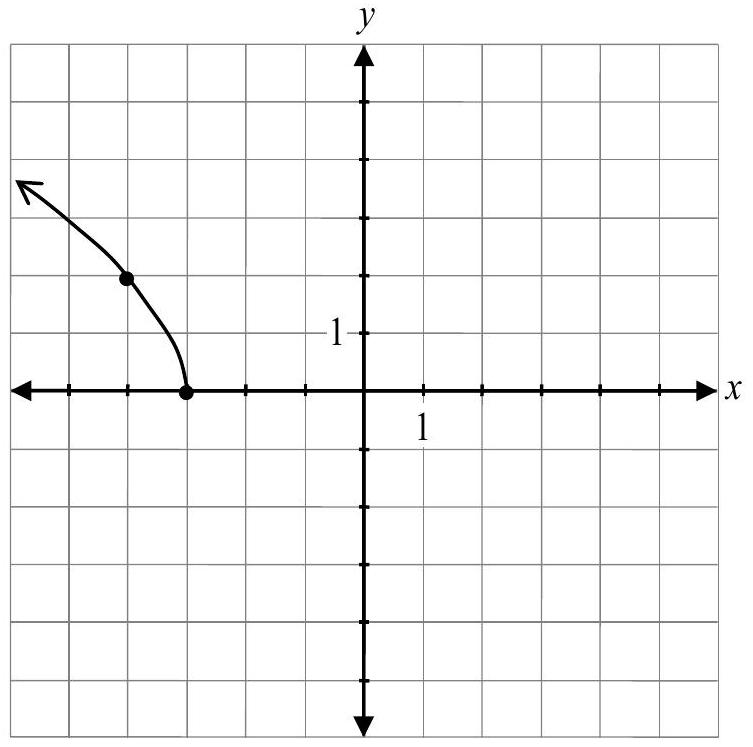
\includegraphics[alt={},max width=\textwidth]{de5fb11a-28c7-4ac7-b7ff-0309cebac724-351_747_753_1069_1134}
\end{center}
\end{figure}

\begin{figure}[h]
\begin{center}
\captionsetup{labelformat=empty}
\caption{C)}
  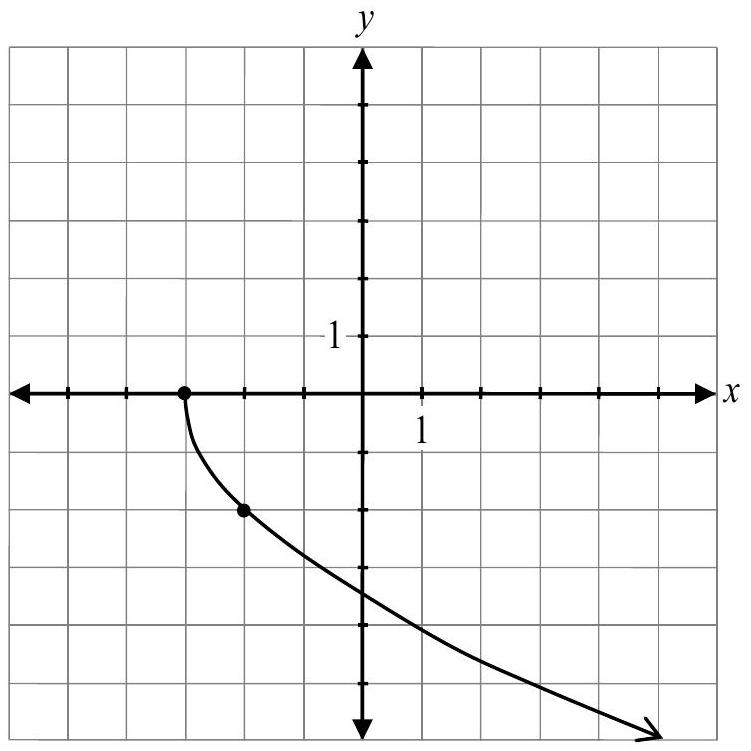
\includegraphics[alt={},max width=\textwidth]{de5fb11a-28c7-4ac7-b7ff-0309cebac724-351_751_751_1851_257}
\end{center}
\end{figure}

\begin{figure}[h]
\begin{center}
\captionsetup{labelformat=empty}
\caption{D)}
  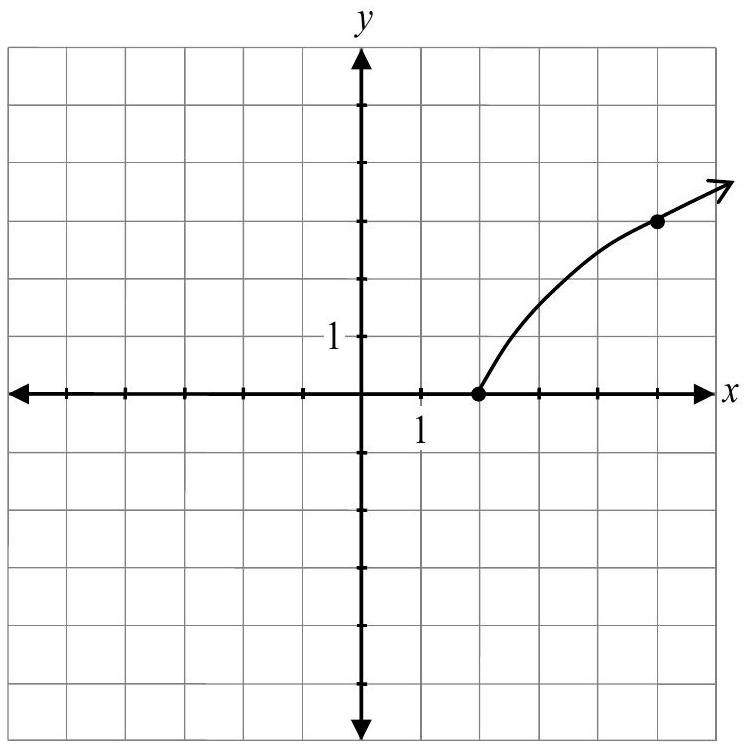
\includegraphics[alt={},max width=\textwidth]{de5fb11a-28c7-4ac7-b7ff-0309cebac724-351_751_749_1851_1138}
\end{center}
\end{figure}

Express $p(x)=x^{3}-2 x^{2}-4 x+8$ as a product of factors.

$$
p(x)=
$$

\section*{Question 29}
a) 3 marks\\
b) 1 mark

Given the graph of $f(x)=(x+3)(x-1)$,\\
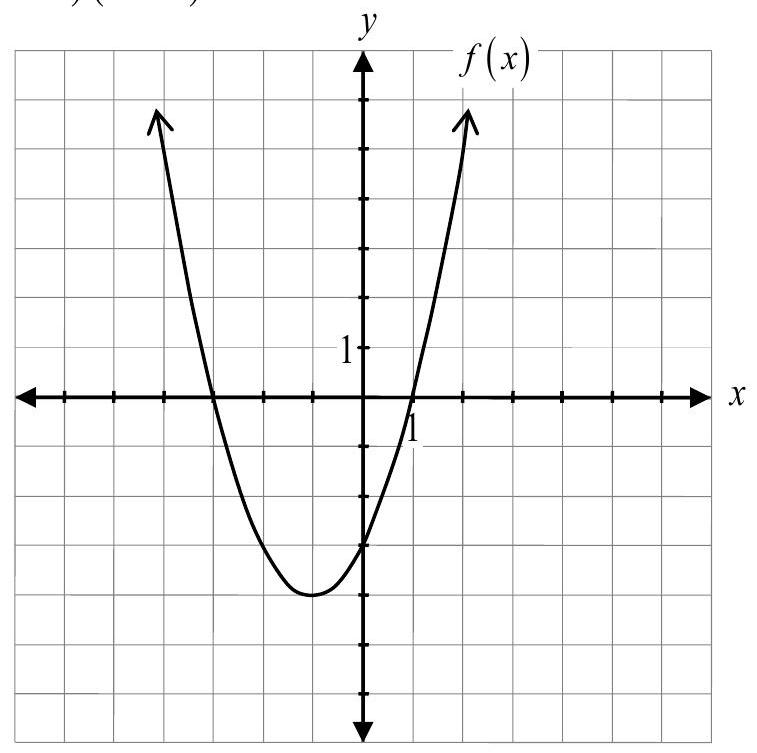
\includegraphics[max width=\textwidth, alt={}, center]{de5fb11a-28c7-4ac7-b7ff-0309cebac724-353_753_757_425_696}\\
a) sketch the graph of $g(x)=\frac{1}{f(x)}$.\\
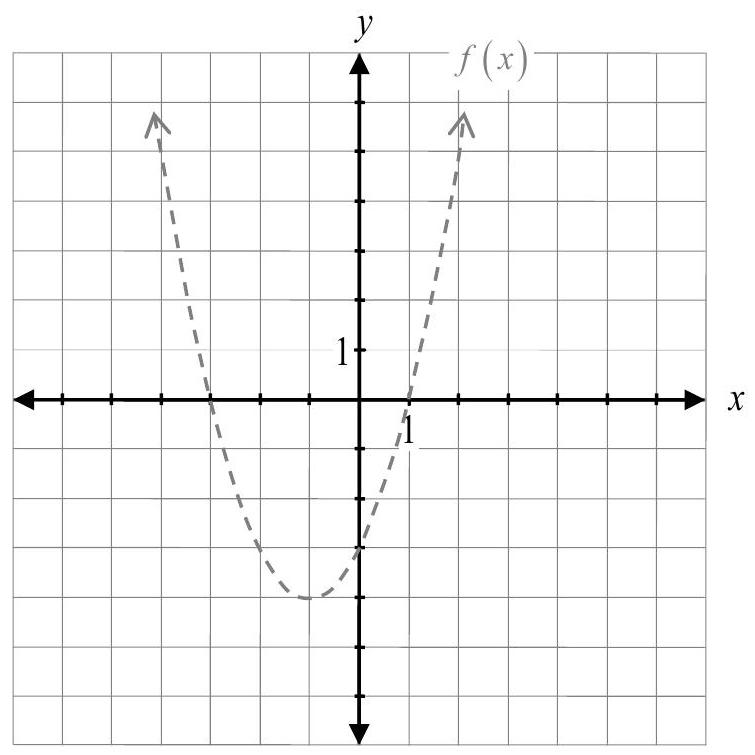
\includegraphics[max width=\textwidth, alt={}, center]{de5fb11a-28c7-4ac7-b7ff-0309cebac724-353_755_755_1327_700}\\
b) describe how to sketch the graph of $h(x)=|f(x)|$.

Describe how the value of $m$ in the equation $y=\log _{3}(x-m), m \in \mathbb{R}$, affects the asymptote on the graph of $y=\log _{3} x$.

Solve algebraically.

$$
25^{x}=\left(\frac{1}{5}\right)^{-3 x+1}
$$

Solve $\cos 2 \theta=0$, where $\theta \in \mathbb{R}$.

Describe a difference between the graphs of $y=f(x)$ and $y=g(x)$.

$$
\begin{aligned}
& f(x)=-2(x+1)^{2}(x+3) \\
& g(x)=2(x+1)^{2}(x+3)
\end{aligned}
$$

Given the graph of $y=f(x)$, sketch the graph of $\sqrt{f(x)}$.\\
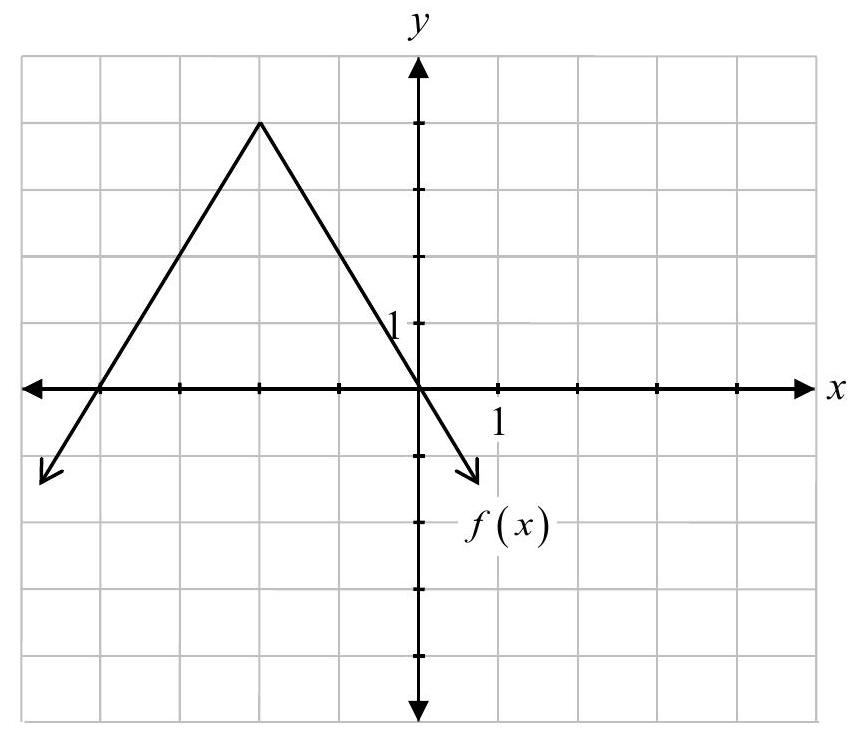
\includegraphics[max width=\textwidth, alt={}, center]{de5fb11a-28c7-4ac7-b7ff-0309cebac724-357_734_861_498_577}\\
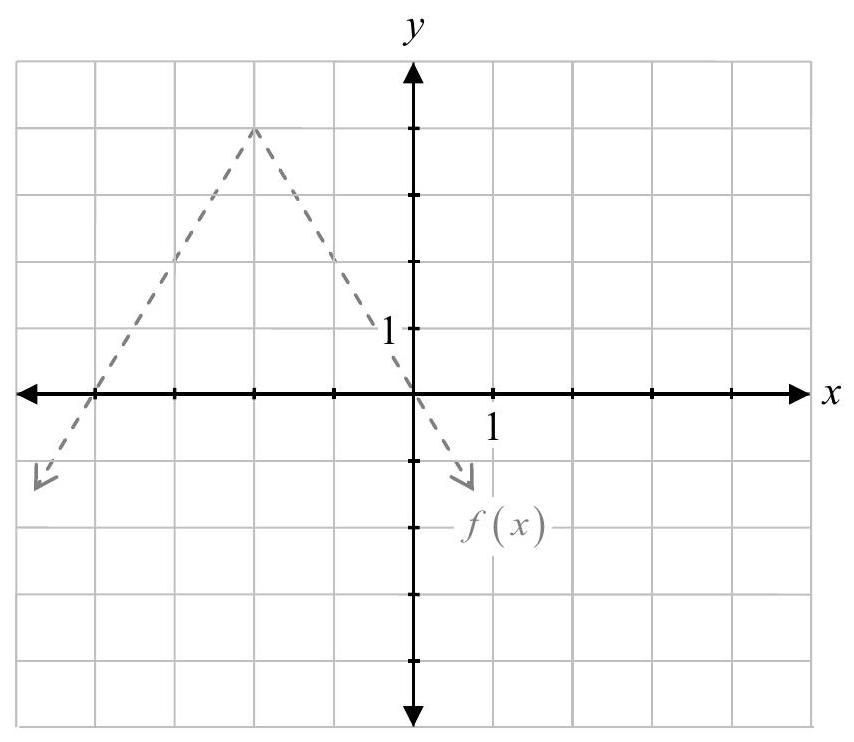
\includegraphics[max width=\textwidth, alt={}, center]{de5fb11a-28c7-4ac7-b7ff-0309cebac724-357_742_854_1465_586}

The graph of $f(x)$ has\\
already been drawn for your reference.\\
No marks will be awarded for the graph of $f(x)$.

Describe the relationship between the zeros of the function $f(x)=(2 x-1)(x+3)^{2}$, the roots of the equation $(2 x-1)(x+3)^{2}=0$, and the $x$-intercepts of the graph of $y=f(x)$.

Question 36

Sketch a graph of at least one period of the function $f(x)=\cos \left[\frac{1}{2}\left(x+\frac{\pi}{2}\right)\right]-3$.\\
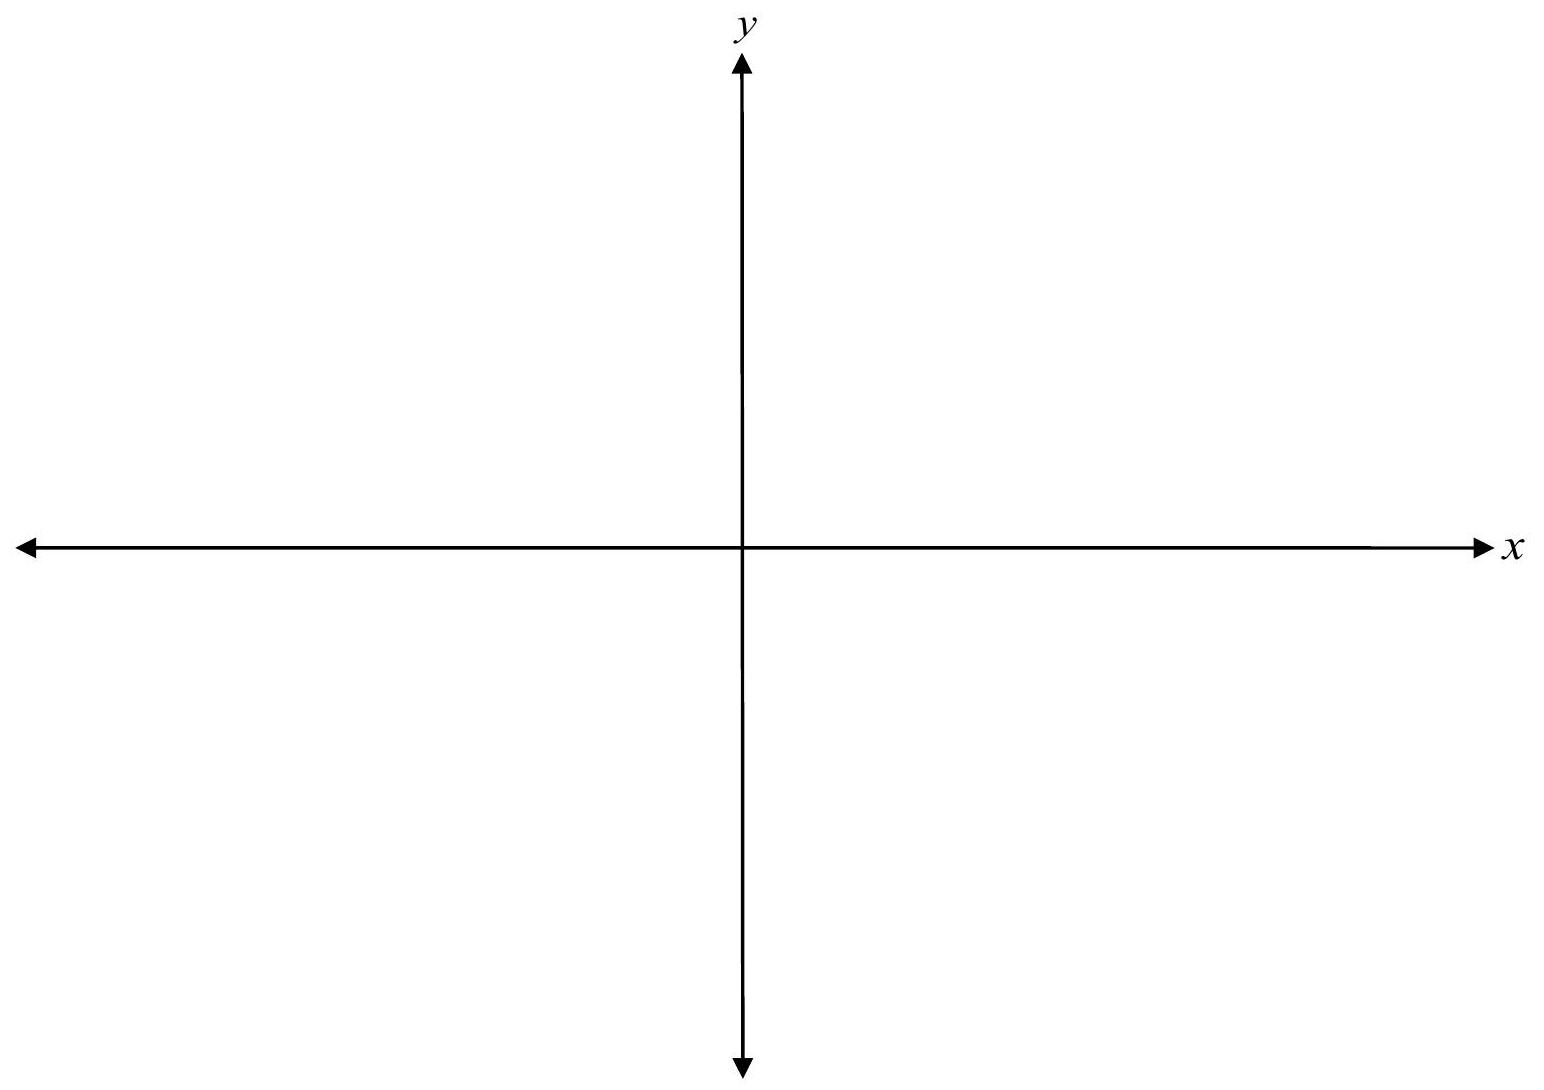
\includegraphics[max width=\textwidth, alt={}, center]{de5fb11a-28c7-4ac7-b7ff-0309cebac724-358_1090_1544_1452_253}

Verify that $\theta=\frac{4 \pi}{3}$ is a solution of the equation $4 \cos ^{2} \theta-1=0$.

Describe how to determine the equation of the horizontal asymptote of a rational function when the degree of the polynomial in the numerator and the degree of the polynomial in the denominator are equal.

Evaluate.

$$
\frac{\cot \left(-\frac{5 \pi}{6}\right)}{\sin \left(\frac{17 \pi}{3}\right)}
$$

Sketch the graph of the function $f(x)=\frac{-1}{(x-1)^{2}}$ and determine the range.\\
\includegraphics[max width=\textwidth, alt={}, center]{de5fb11a-28c7-4ac7-b7ff-0309cebac724-361_876_947_519_302}

Range: $\_\_\_\_$

Given $f(x)=\sqrt{x-2}$ and $g(x)=x^{2}+1$,\\
a) determine $g(f(x))$.

$$
g(f(x))=
$$

b) explain why the domain of $g(f(x))$ is restricted.

Solve algebraically.

$$
2 \log _{a} 3+\log _{a} 4=2, \text { where } a>0
$$

Solve $\sec \theta+2=0$ over the interval $[0,2 \pi]$.

Determine the $x$-intercept of the graph of $f(x)=e^{x}-1$.

\section*{Question 45}
Given the $5^{\text {th }}$ row of Pascal's triangle, determine the values of the next row.

$$
\begin{array}{lllll}
1 & 4 & 6 & 4 & 1
\end{array}
$$

Evaluate.

$$
\log _{2} 80-\log _{2} 10
$$

State the amplitude of $f(x)=-2 \sin (x-\pi)-1$.

Determine the exact value of $\cos 15^{\circ}$.

\section*{Question 49}
a) 1 mark\\
b) 1 mark

Given $f(x)=x^{2}+5 x+6, g(x)=x+3$, and $h(x)=f(x)-g(x)$,\\
a) determine $h(x)$.

$$
h(x)=
$$

$\_\_\_\_$\\
b) sketch the graph of $y=h(x)$.\\
\includegraphics[max width=\textwidth, alt={}, center]{de5fb11a-28c7-4ac7-b7ff-0309cebac724-367_852_876_1428_562}

A group of 7 friends decide to go to a movie.\\
Determine how many ways the friends can sit in a row if two of the friends refuse to sit next to each other.

Gabrielle listens to her radio at a sound level of 80 dB . She attended a music concert that had a sound level of 115 dB . Determine how many times more intense the music concert was than the radio.

You may use the formula:

$$
\beta=10 \log \left(\frac{I}{I_{0}}\right)
$$

where $\quad \beta$ is the intensity level of sound, measured in dB\\
$I$ is the intensity of sound\\
$I_{0}$ is the standard minimum intensity that a person can hear

Solve, algebraically.

$$
2(7)^{x}=3^{2 x-3}
$$

Solve for $\theta$, algebraically, over the interval $[0,2 \pi]$.

$$
\csc ^{2} \theta+2 \csc \theta-8=0
$$

You have forgotten the code to unlock your cell phone. You know the code is made up of four numbers from 0 to 9 .

Determine the number of possible codes, if repetition is allowed.

Note: A calculator is not required for the remaining test questions.

In the binomial expansion of $\left(\frac{7}{x^{3}}-3 x^{7}\right)^{n}$, the $5^{\text {th }}$ term contains $x^{7}$.\\
Determine the value of $n$.

Given the domain of $f(x)$ is $\{-6,1,3,4\}$ and the range of $f(x)$ is $\{-4,7,10,15\}$, state the domain of $f^{-1}(x)$.

Given the graph of $y=f(x)$, sketch the graph of its inverse.\\
\includegraphics[max width=\textwidth, alt={}, center]{de5fb11a-28c7-4ac7-b7ff-0309cebac724-375_723_772_500_696}\\
\includegraphics[max width=\textwidth, alt={}, center]{de5fb11a-28c7-4ac7-b7ff-0309cebac724-375_731_772_1308_696}

The graph of $f(x)$ has already been drawn for your reference.

No marks will be awarded for the graph of $f(x)$.

Prove the following identity for all permissible values of $\theta$.

$$
\frac{1+\cos \theta}{1-\sin ^{2} \theta}=\sec \theta+\tan ^{2} \theta+1
$$

\begin{center}
\begin{tabular}{|l|l|}
\hline
Left-Hand Side & Right-Hand Side \\
\hline
\end{tabular}
\end{center}

Thomas used graphs to solve the equation $e^{x+2}=\sqrt{-(x+1)}$.\\
\includegraphics[max width=\textwidth, alt={}, center]{de5fb11a-28c7-4ac7-b7ff-0309cebac724-377_734_909_485_623}

He incorrectly states the solution as $(-2,1)$.\\
Describe how Thomas should have stated the solution.

Given the graph of $y=f(x)$, sketch the graph of $y=\sqrt{f(x)}$.\\
\includegraphics[max width=\textwidth, alt={}, center]{de5fb11a-28c7-4ac7-b7ff-0309cebac724-378_727_773_483_691}\\
\includegraphics[max width=\textwidth, alt={}, center]{de5fb11a-28c7-4ac7-b7ff-0309cebac724-378_734_777_1325_689}

The graph of $f(x)$ has already been drawn for your reference.\\
No marks will be awarded for the graph of $f(x)$.

When a polynomial, $P(x)$, is divided by ( $x-2$ ) the resulting equation is\\
$\frac{P(x)}{x-2}=x^{2}-x+1+\frac{3}{x-2}$.\\
a) Explain why $x-2$ is not a factor of $P(x)$.\\
b) Determine the equation for the polynomial function $P(x)$.\\
$P(x)=$

Determine the equation for $g(x)$ in terms of $f(x)$.\\
\includegraphics[max width=\textwidth, alt={}, center]{de5fb11a-28c7-4ac7-b7ff-0309cebac724-380_798_839_468_234}\\
\includegraphics[max width=\textwidth, alt={}, center]{de5fb11a-28c7-4ac7-b7ff-0309cebac724-380_798_830_468_1102}\\
$g(x)=$ $\_\_\_\_$

Explain why the binomial expansion of $(2 x+y)^{9}$ does not have a middle term.

Using the laws of logarithms, completely expand the expression $\log \left(\frac{5 \sqrt{a}}{b^{3}}\right)$.

Identify $10^{\circ}$ in radians.\\
a) $\frac{1800}{\pi}$\\
b) $\frac{\pi}{1800}$\\
c) $\frac{18}{\pi}$\\
d) $\frac{\pi}{18}$

\section*{Question 17}
The polynomial function, $P(x)=a(x-1)^{2}(x+4)^{2}$, has a $y$-intercept of -8 .\\
Identify the value of $a$.\\
a) -2\\
b) $-\frac{1}{2}$\\
c) $\frac{1}{2}$\\
d) 2

\section*{Question 18}
Identify the value of $\log _{4}\left(\frac{1}{16}\right)$.\\
a) -2\\
b) $-\frac{1}{2}$\\
c) $\frac{1}{2}$\\
d) 2

\section*{Question 19}
Given the angle $\frac{25 \pi}{7}$, identify the coterminal angle on the interval $[-2 \pi, 0]$.\\
a) $\frac{18 \pi}{7}$\\
b) $\frac{11 \pi}{7}$\\
с) $-\frac{3 \pi}{7}$\\
d) $-\frac{10 \pi}{7}$

\section*{Question 20}
Identify which expression cannot be evaluated.\\
a) ${ }_{7} P_{0}$\\
b) ${ }_{7} P_{6}$\\
c) ${ }_{7} P_{7}$\\
d) ${ }_{7} P_{8}$

\section*{Question 21}
Identify the graph of $f(x)=\frac{-3 x}{2 x+4}$.\\
\includegraphics[max width=\textwidth, alt={}, center]{de5fb11a-28c7-4ac7-b7ff-0309cebac724-385_753_802_586_219}\\
\includegraphics[max width=\textwidth, alt={}, center]{de5fb11a-28c7-4ac7-b7ff-0309cebac724-385_753_777_586_1108}\\
\includegraphics[max width=\textwidth, alt={}, center]{de5fb11a-28c7-4ac7-b7ff-0309cebac724-385_751_759_1396_234}\\
\includegraphics[max width=\textwidth, alt={}, center]{de5fb11a-28c7-4ac7-b7ff-0309cebac724-385_766_772_1392_1108}

Given a point $(-2,0)$ on the graph of $y=f(x)$, identify the coordinates of the corresponding point on the graph of $y=4 f\left(\frac{1}{2} x\right)$.\\
a) $(-8,0)$\\
b) $(-4,0)$\\
c) $(-2,0)$\\
d) $(-1,0)$

Question 23

Identify the non-permissible value of $\theta$ for the expression $\frac{\cos \theta}{1+\sin \theta}$.\\
a) $\frac{\pi}{2}$\\
b) $\pi$\\
c) $\frac{3 \pi}{2}$\\
d) $2 \pi$

Question 24

Identify the function with an asymptote at $x=-3$.\\
a) $y=\log (x+3)$\\
b) $y=\log x+3$\\
c) $y=\log (x-3)$\\
d) $y=\log x-3$

Evaluate the following expression.

$$
\tan \left(\frac{2 \pi}{3}\right) \csc \left(\frac{-2 \pi}{3}\right)+\cos (3 \pi)
$$

State the range of the graph below.\\
\includegraphics[max width=\textwidth, alt={}, center]{de5fb11a-28c7-4ac7-b7ff-0309cebac724-388_894_899_449_625}

Range: $\_\_\_\_$

Sketch the graph of the function $f(x)=\frac{2 x^{2}-5 x}{x}$.\\
\includegraphics[max width=\textwidth, alt={}, center]{de5fb11a-28c7-4ac7-b7ff-0309cebac724-389_843_846_552_661}

State a possible value of $n$ if the polynomial function $P(x)=(x-1)^{2}(x+2)^{n}$ has a range of $[0, \infty)$.

Sketch the graph of $y=\left(\frac{1}{2}\right)^{x-1}$.\\
\includegraphics[max width=\textwidth, alt={}, center]{de5fb11a-28c7-4ac7-b7ff-0309cebac724-391_882_889_552_635}

Solve.

$$
\log _{x} 27=3
$$

Sketch at least two periods of the graph $y=\tan x$.\\
\includegraphics[max width=\textwidth, alt={}, center]{de5fb11a-28c7-4ac7-b7ff-0309cebac724-392_897_1406_1484_333}

Given the graph of $f(x)$, determine the domain of $\frac{1}{f(x)}$.\\
\includegraphics[max width=\textwidth, alt={}, center]{de5fb11a-28c7-4ac7-b7ff-0309cebac724-393_852_854_517_653}

Domain: $\_\_\_\_$

Determine the values of $\mathrm{A}, \mathrm{B}$, and D of the sinusoidal function in the form $y=\mathrm{A} \sin (\mathrm{B} x)+\mathrm{D}$.\\
\includegraphics[max width=\textwidth, alt={}, center]{de5fb11a-28c7-4ac7-b7ff-0309cebac724-394_794_918_500_644}

A = $\_\_\_\_$\\
$\mathrm{B}=$ $\_\_\_\_$

D = $\_\_\_\_$

Determine if the point $\left(-\frac{\sqrt{7}}{5}, \frac{2}{5}\right)$ is on the unit circle.\\
Justify your answer.

Solve, algebraically.

$$
\frac{{ }_{n} C_{5}}{{ }_{n} C_{4}}=6
$$

Given $\sin \alpha=\frac{4}{5}$, where $\alpha$ is in quadrant II, determine the exact value of $\sin 2 \alpha$.

Given the functions $f(x)=x+1$ and $g(x)=\sqrt{x}$,\\
a) determine the equation of $g(f(x))$.

$$
g(f(x))=
$$

$\_\_\_\_$\\
b) sketch the graph of $g(f(x))$.\\
\includegraphics[max width=\textwidth, alt={}, center]{de5fb11a-28c7-4ac7-b7ff-0309cebac724-398_798_805_1014_646}

Steve is asked to determine an equation with a larger period than the period of the graph of $y=\cos (2 x)$.

Justify why Steve's answer of $y=\cos (6 x)$ is incorrect.

Given the graphs of $f(x)$ and $g(x)$,\\
\includegraphics[max width=\textwidth, alt={}, center]{de5fb11a-28c7-4ac7-b7ff-0309cebac724-400_699_727_466_315}\\
\includegraphics[max width=\textwidth, alt={}, center]{de5fb11a-28c7-4ac7-b7ff-0309cebac724-400_701_736_464_1140}\\
a) determine the value of $(f \cdot g)(-1)$.\\
b) determine the value of $g(f(0))$.

Sketch the graph of $P(x)=-(x-1)^{3}(x-3)(x+1)$.\\
\includegraphics[max width=\textwidth, alt={}, center]{de5fb11a-28c7-4ac7-b7ff-0309cebac724-401_894_929_608_590}

The point $(-\sqrt{3}, 1)$ is on the terminal arm of an angle $\theta$, in standard position.\\
a) Determine $\tan \theta$.\\
b) Determine a possible value of $\theta$, in radians.

Describe the transformation used to obtain the graph of $y=\log _{5} x$ given the graph of $y=5^{x}$.

\section*{Question 43}
Solve $\sin \theta=-\frac{\sqrt{3}}{2}$, where $\theta \in \mathbb{R}$.

Given that the point $(a, b)$ is on the graph of $f(x)$, describe how you would determine the corresponding point on the graph of $y=\sqrt{f(x)}$.

Evaluate.

$$
\cos \left(\frac{\pi}{20}\right) \cos \left(\frac{\pi}{5}\right)-\sin \left(\frac{\pi}{20}\right) \sin \left(\frac{\pi}{5}\right)
$$

Describe the transformations used to obtain the graph of the function $y=f(-x+6)-8$ from the graph of $y=f(x)$.

State the equations of all the asymptotes of the function, $y=\frac{1}{3 x+1}$.

Determine the zeros of the polynomial function $P(x)=2 x^{3}+5 x^{2}-4 x-3$.

Determine the equation of the radical function represented by the graph.\\
\includegraphics[max width=\textwidth, alt={}, center]{de5fb11a-28c7-4ac7-b7ff-0309cebac724-407_798_805_519_676}

$$
y=
$$

Pierre pushes his car into a garage. The radius of a tire on his car is 22 cm . Determine the distance travelled by his car if the tire rotated a total of $1000^{\circ}$.

Solve, algebraically.

$$
7^{\frac{x}{2}}=85
$$

Solve, algebraically, over the interval $[0,2 \pi)$.

$$
\sin x(\sec x+3)=0
$$

Brahim invests $\$ 2500$ at an annual interest rate of $6.75 \%$ compounded monthly. Determine, algebraically, how many years it will take for his investment to reach an amount of $\$ 10500$.

Use the formula:

$$
A=P\left(1+\frac{r}{n}\right)^{n t}
$$

where $A=$ the amount of the investment after $t$ years\\
$P=$ the principal of the investment\\
$r=$ the annual interest rate (as a decimal)\\
$n=$ the number of compounding periods per year\\
$t=$ the length of the investment in years

There are 13 adults and 18 children who can be selected to go on a trip. Determine the number of ways 4 adults and 7 children can be selected if Sandra, one of the adults, must be selected.

In the binomial expansion of $\left(\frac{2}{x^{2}}-x^{3}\right)^{9}$, determine and simplify the $6{ }^{\text {th }}$ term.

Note: A calculator is not required for the remaining test questions.

Given that $f(x)=\{(-1,0),(0,2),(1,-3),(2,4)\}$, evaluate $f(f(0))$.

The point $\left(-\frac{5}{6}, b\right)$ is on the unit circle and is in quadrant III.\\
Determine the exact value of $b$.

Given the following row of Pascal's Triangle, determine the values of the next row.

$$
\begin{array}{lllllll}
1 & 6 & 15 & 20 & 15 & 6 & 1
\end{array}
$$

The following transformations are applied to $f(x)$, resulting in a new function, $g(x)$.

\begin{itemize}
  \item reflection over the $x$-axis
  \item vertical stretch by a factor of 3
  \item horizontal stretch by a factor of 4
\end{itemize}

State the equation of $g(x)$ in terms of $f(x)$.

$$
g(x)=
$$

Given the graph of $f(x)$, sketch the graph of $y+1=2 f(x-3)$.\\
\includegraphics[max width=\textwidth, alt={}, center]{de5fb11a-28c7-4ac7-b7ff-0309cebac724-418_800_803_526_663}\\
\includegraphics[max width=\textwidth, alt={}, center]{de5fb11a-28c7-4ac7-b7ff-0309cebac724-418_804_805_1405_663}

The graph of $f(x)$ has already been drawn for your reference.

No marks will be awarded for the graph of $f(x)$

State the equation of the horizontal asymptote of $f(x)=\frac{2 x^{2}-3 x+5}{4 x^{2}+2 x-7}$.

Given that $(x+4)$ is one of the factors of $p(x)=x^{3}+6 x^{2}-32$, express $p(x)$ in completely factored form.\\
$p(x)=$

Prove the identity for all permissible values of $\theta$.

$$
\frac{2 \cos ^{2} \theta}{1-\cot \theta}=\frac{\sin 2 \theta}{\tan \theta-1}
$$

\begin{center}
\begin{tabular}{|l|l|}
\hline
Left-Hand Side & Right-Hand Side \\
\hline
\end{tabular}
\end{center}

Restaurant A has 5 types of hamburgers, 2 types of french fries, and 10 types of drinks. Restaurant B has 4 types of hamburgers, 5 types of french fries, and 6 types of drinks.

If a meal is made up of a hamburger, french fries, and a drink, justify which restaurant offers a greater variety of meals.

Express $\log _{7}(2 x-5)+2 \log _{7} 3$ as a single logarithm.

Explain why 11 ! is not the total number of 11-letter arrangements that can be made from the word CELEBRATION.

Given $f(x)=x-1$, identify a point on the graph of $y=\sqrt{f(x)}$.\\
a) $(0,-1)$\\
b) $(3,2)$\\
c) $(1,0)$\\
d) $(0,1)$

Question 19

Identify the total number of possible arrangements of 6 adults and 4 children seated in a row if the children must sit together.\\
a) $6!4!$\\
b) $7!4$ !\\
c) 10 !\\
d) 6 !

Identify the exact value of $\sec \left(-\frac{7 \pi}{3}\right)$.\\
a) -2\\
b) $-\frac{2}{\sqrt{3}}$\\
c) $\frac{2}{\sqrt{3}}$\\
d) 2

Given $\log _{x}\left(\frac{1}{25}\right)=-2$, identify the value of $x$.\\
a) -5\\
b) $-\frac{1}{5}$\\
c) $\frac{1}{5}$\\
d) 5

Question 22

Identify the equation for all of the asymptotes on the graph of $y=\tan x$.\\
a) $x=k \pi, k \in \mathbb{Z}$\\
b) $x=2 k \pi, k \in \mathbb{Z}$\\
c) $x=\frac{\pi}{2}+k \pi, k \in \mathbb{Z}$\\
d) $x=\frac{\pi}{2}+2 k \pi, k \in \mathbb{Z}$

If $p(x)=3(m)(x+1)^{2}$ is a cubic function with a $y$-intercept of -12 , identify the missing factor, $m$.\\
a) $m=x-4$\\
b) $m=x+4$\\
c) $m=x+12$\\
d) $m=x-12$

Identify the number of negative terms in the binomial expansion of $(x-y)^{5}$.\\
a) 2\\
b) 3\\
c) 5\\
d) 6

Question 25

Given $f(x)=x^{2}$, identify which equation represents the graph of $y=f(x)$ after a translation of 5 units to the left.\\
a) $y=(x+5)^{2}$\\
b) $y=(x-5)^{2}$\\
c) $y=x^{2}-5$\\
d) $y=x^{2}+5$

Question 26

When a polynomial, $p(x)$, is divided by ( $x-7$ ), the remainder is 24 . Identify the only statement that must be true.\\
a) $x=7$ is a zero of $p(x)$\\
b) $p(7)=24$\\
c) $x=24$ is a zero of $p(x)$\\
d) the $y$-intercept is 24

Given $f(x)=\frac{(2 x+1)(x-8)}{(x-8)(x+4)}$, state the equation(s) of the vertical asymptote(s).

Given the graph of $(f \cdot g)(x)$ and $g(x)$, sketch the graph of $f(x)$.\\
\includegraphics[max width=\textwidth, alt={}, center]{de5fb11a-28c7-4ac7-b7ff-0309cebac724-429_798_763_504_262}\\
\includegraphics[max width=\textwidth, alt={}, center]{de5fb11a-28c7-4ac7-b7ff-0309cebac724-429_798_761_504_1102}\\
\includegraphics[max width=\textwidth, alt={}, center]{de5fb11a-28c7-4ac7-b7ff-0309cebac724-429_768_768_1514_253}

Brian was asked to state the zeros of the polynomial $p(x)=(x+2)(x-5)(x-1)$.\\
Brian's response:

$$
\text { Zeros: }(x+2),(x-5),(x-1)
$$

Explain why his response is incorrect.

Simplify ${ }_{n+3} C_{2}$.

Verify that the equation $2 \cos ^{2} x=\sin x+1$ is true for $x=\frac{\pi}{6}$.

The height of a fish jumping out of the water can be modelled by the function $h(t)=-t(t-1)(t-4)(t-5)$ where $h(t)$ is the height of the fish above or below the water in cm , and $t$ is the time in seconds, $t \geq 0$.\\
a) Sketch a graph representing the height of the fish with respect to time over the interval $[0,5]$.\\
\includegraphics[max width=\textwidth, alt={}, center]{de5fb11a-28c7-4ac7-b7ff-0309cebac724-433_936_916_734_661}\\
b) State, from the graph in a), the total number of seconds that the fish is above the water.

Describe the behaviour of the graph of $y=5^{x}+4$ as it approaches $y=4$.

Sketch the angle of 6 radians in standard position.\\
\includegraphics[max width=\textwidth, alt={}, center]{de5fb11a-28c7-4ac7-b7ff-0309cebac724-435_917_1066_577_522}

Sketch the graph of the function $y=4 \sin \left(\frac{\pi}{3} x\right)-2$ over the domain $[-3,6]$.\\
\includegraphics[max width=\textwidth, alt={}, center]{de5fb11a-28c7-4ac7-b7ff-0309cebac724-436_938_1378_571_352}

Given $f(x)=3 x-12$ and $g(x)=x-4$,\\
a) determine the equation of $h(x)=\left(\frac{f}{g}\right)(x)$.

$$
h(x)=
$$

b) describe what the non-permissible value represents on the graph of $h(x)$.

Determine an equation of a radical function, $f(x)$, with a domain of $x \geq 5$ and a range of $y \geq-2$.

$$
f(x)=
$$

Determine the exact value of $\cos \left(\frac{17 \pi}{12}\right)$.

Sketch the graph of $y=\frac{1}{2} \sqrt{-x}+1$.\\
\includegraphics[max width=\textwidth, alt={}, center]{de5fb11a-28c7-4ac7-b7ff-0309cebac724-440_856_872_509_620}

Given $f(x)=\frac{3 x}{4}+9$, determine the equation of $f^{-1}(x)$.

Describe the end behaviour of the polynomial function $p(x)=-(x-2)(x+3)^{2}$.

Given $\csc \theta=-4$ and $\theta$ is in quadrant IV,\\
a) determine the exact value of $\cos \theta$.\\
b) determine the exact value of $\cot \theta$.

Sketch the graph of the function $f(x)=\frac{10}{x^{2}+2}$.\\
\includegraphics[max width=\textwidth, alt={}, center]{de5fb11a-28c7-4ac7-b7ff-0309cebac724-444_921_919_562_605}

Explain why only one of the following equations could be solved algebraically without using logarithms.

$$
3^{5 x}=6^{2 x-1} \quad \text { or } \quad 16^{2 x+3}=\left(\frac{1}{2}\right)^{4 x-5}
$$

Given a graph of $y=f(x)$, describe how to sketch the graph of $y=|f(x)|$.

Sketch the graph of $y=\log _{3}(x+4)$.\\
\includegraphics[max width=\textwidth, alt={}, center]{de5fb11a-28c7-4ac7-b7ff-0309cebac724-447_783_781_485_674}

Solve, algebraically.

$$
\log x+\log 4-\log (x-2)=\log 5
$$

Given $\sin \theta=\frac{1}{2}$, determine all possible values of $\theta$ over the interval $[-2 \pi, 2 \pi]$.

Determine the length of the radius, $r$, given an arc length of 20 metres and a central angle of $160^{\circ}$.\\
\includegraphics[max width=\textwidth, alt={}, center]{de5fb11a-28c7-4ac7-b7ff-0309cebac724-450_287_298_502_833}

There are eight cars parked in a row. Determine the number of possible arrangements of these eight cars if Mrs. Jones must always park in the third spot and Mr. Rodriguez must always park in the last spot.

Bill wins $\$ 1300000$ in a lottery and invests the entire amount at an annual interest rate of $2.5 \%$ compounded quarterly. He will withdraw $\$ 10000$ at the end of every three months.

Determine, algebraically, the total number of withdrawals, including the partial amount, that Bill can make until there is no money left. Express your answer as a whole number.

Use the formula:

$$
P V=\frac{R\left[1-(1+i)^{-n}\right]}{i}
$$

where

$$
\begin{aligned}
P V & =\text { the present value deposited } \\
R & =\text { the amount of each withdrawal } \\
n & =\text { the number of equal withdrawals } \\
i & =\frac{\text { the annual interest rate (in decimal form) }}{\text { the number of compounding periods }}
\end{aligned}
$$

Determine and simplify the $12{ }^{\text {th }}$ term in the binomial expansion of $\left(x^{3}-\frac{1}{2 x^{2}}\right)^{12}$.

Solve, algebraically.

$$
e^{2 x-3}=7^{x+1}
$$

Sketch the angle $\frac{7 \pi}{3}$ in standard position.\\
\includegraphics[max width=\textwidth, alt={}, center]{de5fb11a-28c7-4ac7-b7ff-0309cebac724-455_730_849_562_623}

Determine, algebraically, all of the zeros of the polynomial function $P(x)=x^{4}-5 x^{3}-4 x^{2}+20 x$.

Justify why four of the terms in the binomial expansion of $(-x+y)^{6}$ are positive.

Determine the equation of $g(x)$ in terms of $f(x)$.\\
\includegraphics[max width=\textwidth, alt={}, center]{de5fb11a-28c7-4ac7-b7ff-0309cebac724-458_803_804_489_670}

$$
g(x)=
$$

$\_\_\_\_$

Prove the identity for all permissible values of $x$.

$$
\frac{\sin x+\tan x}{\cot x+\csc x}=\frac{\sin ^{2} x}{\cos x}
$$

\begin{center}
\begin{tabular}{|l|l|}
\hline
Left-Hand Side & Right-Hand Side \\
\hline
 &  \\
\hline
\end{tabular}
\end{center}

Given that the point $(-2,1)$ is on the graph of $y=f(x)$, describe how the coordinates of the corresponding point on the graph of $y=f(4 x)$ are different.

Using the laws of logarithms, completely expand the expression:

$$
\log \left(\frac{x^{2} \sqrt{y}}{w-1}\right)
$$

\section*{Question 13}
Given $\sec \theta=-\frac{5}{4}$ and $\tan \theta>0$, state the quadrant in which $\theta$ terminates.\\
Justify your answer.

State an equation of a rational function that has a vertical asymptote at $x=-8$ and a horizontal asymptote at $y=9$.

\section*{Question 15}
Given the point $(5,1)$, state the coordinates of the corresponding point after a reflection across the line $y=x$.

Simplify.

$$
\frac{(n-13)!}{(n-12)!}
$$

\section*{Question 17}
a) 1 mark b) 1 mark

Given the graphs of $y=f(x)$ and $y=g(x)$,\\
\includegraphics[max width=\textwidth, alt={}, center]{de5fb11a-28c7-4ac7-b7ff-0309cebac724-464_652_656_455_380}\\
\includegraphics[max width=\textwidth, alt={}, center]{de5fb11a-28c7-4ac7-b7ff-0309cebac724-464_652_656_455_1095}\\
a) determine the value of $f(g(2))$.\\
b) determine the value of $(g-f)(-3)$.

Identify the remainder when $P(x)=3 x^{3}-x^{2}+1$ is divided by $(x-2)$.\\
a) -27\\
b) -19\\
c) 11\\
d) 21

\section*{Question 19}
Identify the logarithmic form of $2^{x}=\frac{1}{4}$.\\
a) $\log _{2} x=\frac{1}{4}$\\
b) $\log _{x} 2=\frac{1}{4}$\\
c) $\log _{2}\left(\frac{1}{4}\right)=x$\\
d) $\log _{x}\left(\frac{1}{4}\right)=2$

Leah's Pizzeria offers 9 different pizza toppings. Identify the expression that represents the number of different types of pizzas, with 3 different toppings, that can be made.\\
a) ${ }_{9} C_{3}$\\
b) ${ }_{9} P_{3}$\\
c) $\frac{9!}{3!}$\\
d) $9!3!$

Given $(5,-4)$ is a point on the graph of $y=f(x)$, identify the corresponding point on the graph of $y=\frac{1}{f(x)}$.\\
a) $\left(\frac{1}{5},-4\right)$\\
b) $\left(5,-\frac{1}{4}\right)$\\
c) $\left(\frac{1}{5},-\frac{1}{4}\right)$\\
d) $(-4,5)$

Question 22

Identify the non-permissible value of $x$ for $1+\sec x$ over $[0, \pi]$.\\
a) 0\\
b) $\frac{\pi}{4}$\\
c) $\frac{\pi}{2}$\\
d) $\pi$

Indicate the combination that represents the circled term in the given row of Pascal's triangle.\\
1\\
46\\
(4) 1\\
a) ${ }_{4} C_{3}$\\
b) ${ }_{4} C_{4}$\\
c) ${ }_{5} C_{3}$\\
d) ${ }_{5} C_{4}$

Identify the $x$-intercept on the graph of $f(x)=\sqrt{2(x+5)}$.\\
a) -5\\
b) 0\\
c) $\sqrt{10}$\\
d) 5

Question 25

Identify the coterminal angle of $\frac{\pi}{5}$ over the interval $-\pi \leq \theta \leq 4 \pi$.\\
a) $-\frac{9 \pi}{5}$\\
b) $-\frac{\pi}{5}$\\
c) $\frac{3 \pi}{5}$\\
d) $\frac{11 \pi}{5}$

Given $f(x)=\{(2,6),(3,2),(3,4),(6,5)\}$, identify the value of $f(f(2))$.\\
a) 3\\
b) 4\\
c) 5\\
d) 6

The graph of $f(x)=(x-1)^{2}$ is translated 2 units to the left and 3 units up. Identify the equation of the transformed graph, $g(x)$.\\
a) $g(x)=(x+1)^{2}+3$\\
b) $g(x)=(x-3)^{2}+3$\\
c) $g(x)=(x+2)^{2}+3$\\
d) $g(x)=(x-2)^{2}+3$

Given $\csc \theta=-\frac{8}{5}$, determine the exact value of $\cos 2 \theta$.

Determine the period of the sinusoidal function, $f(x)=-6 \cos \left(\frac{\pi}{6}(x+1)\right)+5$.

Determine, algebraically, the equation of $P(x)$, given the graph of the polynomial function $P(x)$.\\
\includegraphics[max width=\textwidth, alt={}, center]{de5fb11a-28c7-4ac7-b7ff-0309cebac724-471_998_843_487_625}\\
$P(x)=$ $\_\_\_\_$

Solve $2 \sin ^{2} \theta-7 \sin \theta-4=0$ where $\theta \in \mathbb{R}$.

Justify that the shapes of the graphs of $f(x)=(x+1)^{2}(x-1)$ and $g(x)=(x+1)^{2}(x-1)^{3}$ are different as they approach the $x$-intercept at $x=1$.

Determine the exact value of $\cot \theta$ if $\cos \theta=-\frac{4}{7}$ and $\sin \theta$ is positive.

Sketch the graph of $f(x)=-\log _{2}(x)+2$.\\
\includegraphics[max width=\textwidth, alt={}, center]{de5fb11a-28c7-4ac7-b7ff-0309cebac724-475_798_803_554_661}

State the range of $f(x)=\sqrt{x+4}$.

\section*{Range:}
Sophie correctly solved the logarithmic equation, $\log _{7}(x-1)=\log _{7}(2 x-2)$.

$$
\begin{aligned}
x-1 & =2 x-2 \\
-1+2 & =2 x-x
\end{aligned}
$$

Explain why $x=1$ is an extraneous root.

Sketch the graph of $f(x)=\sqrt{4 x}-1$.\\
\includegraphics[max width=\textwidth, alt={}, center]{de5fb11a-28c7-4ac7-b7ff-0309cebac724-478_794_802_640_644}

Solve, algebraically.

$$
{ }_{n} C_{2}=2 n+7
$$

Given $f(x)=x^{2}-1$ and $g(x)=x-3$, explain why the domain of $h(x)=\frac{f(x)}{g(x)}$ has a restriction when $x=3$.

Evaluate.

$$
\frac{\cot \left(\frac{11 \pi}{6}\right) \sin \left(-\frac{4 \pi}{3}\right)}{\cos \left(\frac{2 \pi}{3}\right)}
$$

Solve, algebraically.

$$
\log _{2}\left(\log _{3} x\right)=2
$$

Sketch the graph of the function $y=5 \sin \left(\frac{\pi}{4} x\right)+1$ over the domain $[-4,8]$.\\
\includegraphics[max width=\textwidth, alt={}, center]{de5fb11a-28c7-4ac7-b7ff-0309cebac724-483_1109_1642_595_225}

Given the graph of $y=f(x)$, sketch the graph of $y=|f(-x)|$.\\
\includegraphics[max width=\textwidth, alt={}, center]{de5fb11a-28c7-4ac7-b7ff-0309cebac724-484_796_802_534_644}\\
\includegraphics[max width=\textwidth, alt={}, center]{de5fb11a-28c7-4ac7-b7ff-0309cebac724-484_807_802_1413_640}

The graph of\\
\includegraphics[max width=\textwidth, alt={}, center]{de5fb11a-28c7-4ac7-b7ff-0309cebac724-484_89_91_1594_1770}\\
$f(x)$ has already been drawn for your reference.\\
No marks will be awarded for the graph of $f(x)$.

Savannah used the graph of $y=f(x)$ to sketch the graph of $y=\sqrt{f(x)}$. Her solution is given below. Describe her error.\\
\includegraphics[max width=\textwidth, alt={}, center]{de5fb11a-28c7-4ac7-b7ff-0309cebac724-485_884_1069_605_554}

Determine the exact value of $\sin \left(\frac{13 \pi}{12}\right)$.

State the equation of the horizontal asymptote of $f(x)=\frac{3 x}{x-1}$.

Sketch the graph of $f(x)=\frac{5 x-10}{x^{2}+x-6}$.\\
\includegraphics[max width=\textwidth, alt={}, center]{de5fb11a-28c7-4ac7-b7ff-0309cebac724-488_802_804_655_696}

Determine, algebraically, the inverse of $f(x)=3 x+4$.

Sketch the graph of $P(x)=-(x+1)(x-2)(x+3)$.\\
\includegraphics[max width=\textwidth, alt={}, center]{de5fb11a-28c7-4ac7-b7ff-0309cebac724-490_843_841_545_646}

Avery has 4 adventure books, 5 mystery books, and 1 comic book.\\
Determine the number of ways he can arrange all of the books on his shelf if each type of book must be grouped together.

Solve the following equation, algebraically, over the interval $[0,2 \pi]$.

$$
5 \cos ^{2} \theta-\cos \theta-\sin ^{2} \theta=0
$$

Given that $-6048 x^{2} y^{5}$ is the sixth term in the expansion of $(3 x-m)^{7}$, determine $m$.

A series of blood tests measures the concentration of a prescribed drug. This concentration decreases according to the formula $A=P e^{r t}$ where:\\
$A$ is the concentration at time $t$\\
$P$ is the initial concentration\\
$r$ is the rate of change\\
$t$ is the time, in hours, after the first blood test\\
The initial concentration is 3.8900 units $/ \mathrm{mL}$. Three hours later, the concentration is 1.7505 units $/ \mathrm{mL}$.\\
a) Determine the rate of change, $r$, algebraically.\\
b) Determine the concentration of the prescribed drug four hours after the initial concentration of 3.8900 units $/ \mathrm{mL}$ was measured. Express the answer correct to 4 decimal places.

Note: A calculator is not required for the remaining test questions.

Ariane uses the formula $s=\theta r$ to determine the arc length of a circle that has a central angle of $20^{\circ}$ and a radius of 15 cm .

Below is Ariane's work:

$$
\begin{aligned}
& S=\theta r \\
& S=(20)(15) \\
& S=300 \mathrm{~cm}
\end{aligned}
$$

Describe her error.

Using the graphs below, state the solution of the equation $2 x+3=2 \sqrt{-x}-1$.\\
\includegraphics[max width=\textwidth, alt={}, center]{de5fb11a-28c7-4ac7-b7ff-0309cebac724-496_891_916_459_601}

Solve, algebraically.

$$
\log _{2}(x+3)=5-\log _{2}(x-1)
$$

Explain why the value of $n$ must be greater than or equal to the value of $r$, when using $C_{n}$.

\section*{Question 9}
3 marks\\
110\\
Given that $y=|x|$, determine the equation of the resulting function, $g(x)$, after the following transformations:

\begin{itemize}
  \item reflection in the $x$-axis
  \item vertical translation 5 units down
  \item horizontal stretch by a factor of 3\\
$g(x)=$
\end{itemize}

Explain why the graph of $y=\frac{x-1}{x^{2}+x-6}$ has a horizontal asymptote at $y=0$.

\section*{Question 11}
Given the graphs of $f(x)$ and $g(x)$, evaluate $g(f(2))$.\\
\includegraphics[max width=\textwidth, alt={}, center]{de5fb11a-28c7-4ac7-b7ff-0309cebac724-499_822_826_1417_285}

Kennedy was asked to solve the equation $\tan \theta=1$ over all real numbers.\\
Below is Kennedy's solution:

$$
\begin{aligned}
& \tan \theta=1 \\
& \theta=\frac{\pi}{4}, \frac{5 \pi}{4}
\end{aligned}
$$

Describe her error.

Solve, algebraically.

$$
{ }_{n} C_{3}=3\left({ }_{n} P_{2}\right)
$$

Given the graph of $y=f(x)$, sketch the graph of $y=\sqrt{f(x)}$.\\
\includegraphics[max width=\textwidth, alt={}, center]{de5fb11a-28c7-4ac7-b7ff-0309cebac724-502_888_936_485_592}\\
\includegraphics[max width=\textwidth, alt={}, center]{de5fb11a-28c7-4ac7-b7ff-0309cebac724-502_897_942_1486_592}

The graph of $f(x)$ has already been drawn for your reference. No marks will be awarded for the graph of $f(x)$.

Prove the identity for all permissible values of $\theta$.

$$
\frac{\sec \theta-\tan \theta \sin \theta}{\tan \theta \sin \theta}=\csc ^{2} \theta-1
$$

\begin{center}
\begin{tabular}{|l|l|}
\hline
Left-Hand Side & Right-Hand Side \\
\hline
\end{tabular}
\end{center}

Sketch the angle of $-\frac{\pi}{12}$ radians in standard position.\\
\includegraphics[max width=\textwidth, alt={}, center]{de5fb11a-28c7-4ac7-b7ff-0309cebac724-504_734_849_534_653}

\section*{Question 17}
Given that $h(x)=2 x^{2}-7 x-15$, determine possible equations of the functions $f(x)$ and $g(x)$ if $h(x)=f(x) \cdot g(x)$.\\
$f(x)=$ $\_\_\_\_$\\
$g(x)=$ $\_\_\_\_$

The range of $y=f(x)$ is $-6 \leq y \leq 12$. The range of the transformed function $y=a f(x)$ is $-2 \leq y \leq 4$. Identify the value of $a$.\\
a) -3\\
b) $-\frac{1}{3}$\\
c) $\frac{1}{3}$\\
d) 3

Question 19

Identify the expression which is equivalent to $3 \log y-\frac{1}{2} \log x+\log z$.\\
a) $\log \left(\frac{y^{3}}{\sqrt{x} z}\right)$\\
b) $\log \left(\frac{y^{3} z}{\sqrt{x}}\right)$\\
c) $\log \left(\frac{y^{3}}{x^{2} z}\right)$\\
d) $\log \left(\frac{y^{3} z}{x^{2}}\right)$

Identify the measure of the angle $-\frac{2 \pi}{9}$ in degrees.\\
a) $-400^{\circ}$\\
b) $-40^{\circ}$\\
c) $40^{\circ}$\\
d) $320^{\circ}$

If $y=f(x)$ has a domain of [2,5] and a range of [6,10], identify the domain of $y=f^{-1}(x)$.\\
a) $\left[\frac{1}{2}, \frac{1}{5}\right]$\\
b) $[-5,-2]$\\
c) $[-10,-6]$\\
d) $[6,10]$

Question 22

Identify which of the following is a polynomial function.\\
a) $p(x)=-\frac{1}{2}(x+2)^{3}(x-3)$\\
b) $p(x)=2 x^{\frac{1}{2}}+x-3$\\
c) $p(x)=3 x^{-4}+x^{2}-6$\\
d) $p(x)=2^{x}+3$

Identify the total number of terms in the expansion of $(x-y)^{9}$.\\
a) 8\\
b) 9\\
c) 10\\
d) 11

Identify the exact value of $2 \cos ^{2}\left(15^{\circ}\right)-1$.\\
a) 1\\
b) $\frac{1}{2}$\\
c) $\frac{\sqrt{3}}{2}$\\
d) $\sqrt{3}$

Question 25

The zeros of the function $y=f(x)$ are $x=-2$ and $x=3$. Identify the zeros of the function $g(x)=2 f(x-4)$.\\
a) $x=-6$ and $x=-1$\\
b) $x=2$ and $x=7$\\
c) $x=-4$ and $x=6$\\
d) $x=0$ and $x=10$

Question 26

Identify the value of $\log _{4}\left(\frac{1}{4}\right)$.\\
a) -16\\
b) -1\\
c) 1\\
d) 16

Sketch the graph of at least one period of the function $y=-\cos \left(x+\frac{\pi}{4}\right)+3$.\\
\includegraphics[max width=\textwidth, alt={}, center]{de5fb11a-28c7-4ac7-b7ff-0309cebac724-508_1071_1567_504_266}

Justify that $(x-5)$ is not a possible factor of the function $P(x)=x^{3}-3 x^{2}-4 x+12$.

Sketch the graph of $f(x)=\frac{6}{(x+2)(x-3)}$ and state the $y$-intercept.\\
\includegraphics[max width=\textwidth, alt={}, center]{de5fb11a-28c7-4ac7-b7ff-0309cebac724-510_1292_1301_571_259}\\
$y$-intercept: $\_\_\_\_$

Determine how many 3 -digit odd numbers less than 300 are possible using the digits $1,2,3,4,5,6$ if repetition is not allowed.

Given that $\cos \alpha=-\frac{5}{13}$ and $\sin \beta=\frac{2}{3}$, where $\alpha$ and $\beta$ terminate in the same quadrant,\\
determine the exact value of $\cos (\alpha-\beta)$. determine the exact value of $\cos (\alpha-\beta)$.

Given the graph of $y=4^{x}$, sketch the graph of $y=2(4)^{x-3}+1$.\\
\includegraphics[max width=\textwidth, alt={}, center]{de5fb11a-28c7-4ac7-b7ff-0309cebac724-513_833_957_534_571}\\
\includegraphics[max width=\textwidth, alt={}, center]{de5fb11a-28c7-4ac7-b7ff-0309cebac724-513_831_951_1486_573}

The graph of $f(x)$ has already been drawn for your reference.\\
No marks will be awarded for the graph of $f(x)$.

Determine the coterminal angle of $\frac{\pi}{5}$ over the interval $[-2 \pi, 0]$.

\section*{Question 34}
State the domain of the graph of $y=\log (x-4)-8$.

Given the graph of $y=5 \sin \left[2\left(x+\frac{\pi}{4}\right)\right]-3$, determine the exact value of the $x$-coordinate in the point P .\\
\includegraphics[max width=\textwidth, alt={}, center]{de5fb11a-28c7-4ac7-b7ff-0309cebac724-515_970_832_573_554}

Verify that the following equation is true for $x=\frac{5 \pi}{6}$.

$$
\frac{\cos x}{1-\sin x}=\frac{1+\sin x}{\cos x}
$$

\begin{center}
\begin{tabular}{|l|l|}
\hline
Left-Hand Side & Right-Hand Side \\
\hline
 &  \\
\hline
\end{tabular}
\end{center}

Given that $(x+1)$ is one of the factors of $P(x)=x^{3}-x^{2}+k x-8$, determine the value of $k$.

Given the function $f(x)=\sqrt{x}$, describe how to use transformations to determine the domain of the function $g(x)=f(x+2)+1$.

Given the graph of $y=f(x)$, state the equation of the vertical asymptote of $y=\frac{1}{f(x)}$.\\
\includegraphics[max width=\textwidth, alt={}, center]{de5fb11a-28c7-4ac7-b7ff-0309cebac724-519_854_862_500_610}

Solve, algebraically.

$$
16^{x}=64^{2 x-1}
$$

Given one of the factors of $P(x)=x^{3}+2 x^{2}-5 x-6$ is ( $x+3$ ), express $P(x)$ in completely factored form.

$$
P(x)=
$$

Sketch the graph of $p(x)=3(x+1)^{2}(x-2)^{2}$.\\
\includegraphics[max width=\textwidth, alt={}, center]{de5fb11a-28c7-4ac7-b7ff-0309cebac724-522_1017_1120_584_507}

Given that $f(x)=x^{2}-4$ and $g(x)=\sqrt{x}$, determine $f(g(x))$ and state its domain.

$$
f(g(x))=
$$

Determine a possible equation of the function $f(x)$.\\
\includegraphics[max width=\textwidth, alt={}, center]{de5fb11a-28c7-4ac7-b7ff-0309cebac724-524_826_828_545_281}

$$
f(x)=
$$

Explain why the graph of $y=\log _{2} x$ does not have a $y$-intercept.

Evaluate.

$$
\sin ^{2}\left(-\frac{\pi}{3}\right)+\cos \left(\frac{17 \pi}{6}\right) \sec \left(\frac{\pi}{6}\right)
$$

Determine the coordinates of the point of discontinuity (hole) on the graph of $y=\frac{x^{2}-3 x}{x}$.

Given the graphs of $f(x)$ and $g(x)$, sketch the graph of $h(x)=f(x)+g(x)$.\\
\includegraphics[max width=\textwidth, alt={}, center]{de5fb11a-28c7-4ac7-b7ff-0309cebac724-528_851_800_466_253}\\
\includegraphics[max width=\textwidth, alt={}, center]{de5fb11a-28c7-4ac7-b7ff-0309cebac724-528_792_794_1430_253}

Given that $\csc \theta=-\frac{4}{\sqrt{7}}$ and $\cos \theta>0$, determine the exact value of $\tan \theta$.

Determine and simplify the $8^{\text {th }}$ term in the binomial expansion of $\left(x-\frac{2}{x^{3}}\right)^{10}$.

The temperature of hot chocolate is recorded as it cools down. The data shows that the temperature cools according to the equation:

$$
T=82(0.87)^{t}+16
$$

where $T$ is the temperature of the hot chocolate, in degrees Celsius after $t$ minutes and $t$ is the time, in minutes, after the hot chocolate is made.

In order to avoid burns, hot chocolate should not be served at a temperature higher than $71^{\circ} \mathrm{C}$. Determine, algebraically, the amount of time it will take the hot chocolate to reach this temperature.

Solve for $\theta$, algebraically, over the interval $[0,2 \pi]$.

$$
3 \sin ^{2} \theta+6 \sin \theta+2=0
$$

A committee of 4 people is to be selected from 6 high school students and 5 middle years students.

Determine the number of possible committees if the committee must have at least 3 high school students.

Given the graph of $y=f(x)$, sketch the graph of $y=-|f(x)|$.\\
\includegraphics[max width=\textwidth, alt={}, center]{de5fb11a-28c7-4ac7-b7ff-0309cebac724-534_804_802_524_627}\\
\includegraphics[max width=\textwidth, alt={}, center]{de5fb11a-28c7-4ac7-b7ff-0309cebac724-534_808_811_1463_623}

The graph of $f(x)$ has already been drawn for your reference.\\
No marks will be awarded for the graph of $f(x)$.

Describe the transformations used to obtain the graph of the function $y=4 f\left(\frac{x}{2}\right)-3$ from the graph of $y=f(x)$.

If $\log 4=m$ and $\log 3=n$, express $\log 48$ in terms of $m$ and $n$.

State the domain and range of the radical function, $f(x)=-3 \sqrt{x-8}+1$.

Domain: $\_\_\_\_$

Range: $\_\_\_\_$

Explain why the graph of $y=\tan x$ does not have an amplitude.

Prove the following identity for all permissible values of $\theta$.

$$
\frac{\sec \theta-\sin ^{2} \theta \sec \theta}{\tan \theta \sin \theta}=\csc ^{2} \theta-1
$$

\begin{center}
\begin{tabular}{|l|l|}
\hline
Left-Hand Side & Right-Hand Side \\
\hline
\end{tabular}
\end{center}

Given that $x=3$ is one of the zeros of $p(x)=x^{3}-7 x-6$, express $p(x)$ in completely factored form.\\
$p(x)=$

Solve, algebraically.

$$
{ }_{n+1} P_{2}=6
$$

Express $\log (3 x-1)-\log x+\log 9$ as a single logarithm.

Sketch the graph of $P(x)=-(x-2)^{2}(x+3)$.\\
\includegraphics[max width=\textwidth, alt={}, center]{de5fb11a-28c7-4ac7-b7ff-0309cebac724-543_1204_1049_528_526}

Given $f(x)=-2 x-5$ and $g(x)=x+7$, identify the equation of $h(x)=f(g(x))$.\\
a) $h(x)=-2 x^{2}-35$\\
b) $h(x)=-2 x-19$\\
c) $h(x)=-2 x^{2}-19 x-35$\\
d) $h(x)=-2 x+2$

\section*{Question 16}
The function $y=f(x)$ has a domain of [2,5] and a range of [-6,3]. Identify the range of the function $y=f^{-1}(x)$.\\
a) $[-6,3]$\\
b) $[-5,2]$\\
c) $[-3,6]$\\
d) $[2,5]$

Question 17

Identify the function that has a graph with a point of discontinuity (hole) at $x=-3$.\\
a) $y=\frac{x+3}{x^{2}-9}$\\
b) $y=\frac{x-3}{x^{2}-9}$\\
c) $y=\frac{x^{2}-9}{x-3}$\\
d) $y=\frac{x^{2}+9}{x+3}$

Identify the value of $\ln e$.\\
a) 0\\
b) $\log e$\\
c) 1\\
d) $e$

Question 19

When the polynomial function, $p(x)$, is divided by ( $x-4$ ) the remainder is 17 . Identify which statement is true.\\
a) $p(4)=17$\\
b) $p(-4)=17$\\
c) $p(4)=0$\\
d) $p(-4)=0$

Question 20

Identify the expression equivalent to $\frac{(n-6)!}{(n-4)!}$.\\
a) $(n-4)(n-5)$\\
b) $\frac{1}{(n-4)(n-5)}$\\
c) $(n-6)(n-5)$\\
d) $\frac{1}{(n-6)(n-5)}$

Identify the quadrant in which $\theta$ terminates if $\sec \theta=-\frac{4}{3}$ and $\sin \theta>0$.\\
a) I\\
b) II\\
c) III\\
d) IV

Question 22

Identify the expression that represents all angles that are coterminal with $\frac{\pi}{3}$.\\
a) $\frac{\pi}{3}+\pi k, k \in \mathbb{Z}$\\
b) $\frac{\pi}{3}+\pi k, k \in \mathbb{R}$\\
c) $\frac{\pi}{3}+2 \pi k, k \in \mathbb{Z}$\\
d) $\frac{\pi}{3}+2 \pi k, k \in \mathbb{R}$

\section*{Given $f(x)=\frac{1}{2} x-3$, state the coordinates of an invariant (unchanged) point when sketching the graph of $y=\sqrt{f(x)}$.}
Solve, algebraically.

$$
125^{3 x+4}=\left(\frac{1}{5}\right)^{x}
$$

Given $\sin \theta=-\frac{\sqrt{2}}{2}$ and $\cos \theta=-\frac{\sqrt{2}}{2}$, justify that the value of $\tan (2 \theta)$ is undefined.

Sketch the graph of $y=-2 \log _{3} x$.\\
\includegraphics[max width=\textwidth, alt={}, center]{de5fb11a-28c7-4ac7-b7ff-0309cebac724-550_916_908_541_586}

Evaluate.

$$
\cos \left(\pi \cdot \sin \left(-\frac{\pi}{6}\right)\right)
$$

a) Given $f(x)=-x+2$, sketch the graph of $h(x)=f(f(x))$.\\
\includegraphics[max width=\textwidth, alt={}, center]{de5fb11a-28c7-4ac7-b7ff-0309cebac724-552_847_858_541_614}\\
b) Explain why the domain of $h(x)=f(f(x))$ does not have any restrictions.\\
a) Sketch the graph of $f(x)=\frac{3 x-5}{2 x+4}$.\\
\includegraphics[max width=\textwidth, alt={}, center]{de5fb11a-28c7-4ac7-b7ff-0309cebac724-553_955_961_552_558}\\
b) State the range of $f(x)$.

Range: $\_\_\_\_$

Determine, algebraically, the equation of $p(x)$ that satisfies all of the following conditions:

\begin{itemize}
  \item $p(x)$ is a polynomial function of degree 4
  \item $p(x)$ has a zero at 3 with a multiplicity of 2
  \item $p(x)$ has zeroes at -1 and -2
  \item $p(x)$ passes through the point $(2,24)$.\\
$p(x)=$
\end{itemize}

Verify, by substitution, that the equation $\frac{\cos \theta+\cot \theta}{\cot \theta}=1+\sin \theta$ is true for $\theta=\frac{2 \pi}{3}$.

\begin{center}
\begin{tabular}{|l|l|}
\hline
Left-Hand Side & Right-Hand Side \\
\hline
 &  \\
\hline
\end{tabular}
\end{center}

Jyugo was asked to state the equation of the vertical asymptote(s) on the graph of $f(x)=\frac{3 x-15}{x^{2}-5 x}$.

His solution:

$$
\begin{array}{r}
f(x)=\frac{3(x-5)}{x(x-5)} \\
x=0 \quad x=5
\end{array}
$$

Explain why his solution is incorrect.

Sketch the graph of $y=\sin \left(\frac{1}{2} x\right)-1$ over the interval $[-2 \pi, 2 \pi]$.\\
\includegraphics[max width=\textwidth, alt={}, center]{de5fb11a-28c7-4ac7-b7ff-0309cebac724-557_826_1599_524_277}

Sketch the graph of $y=\sqrt{-2 x+6}$.\\
\includegraphics[max width=\textwidth, alt={}, center]{de5fb11a-28c7-4ac7-b7ff-0309cebac724-558_779_792_575_646}

Determine the measure of angle R , in radians.

\section*{Question 36}
Given $f(x)=\sqrt{x-4}$, state the equation of the resulting function, $g(x)$, after a reflection over the $x$-axis.

$$
g(x)=
$$

$\_\_\_\_$\\
a) Determine the coterminal angle of $\frac{29 \pi}{12}$ over the interval $[0,2 \pi]$.\\
b) Determine the exact value of $\sin \left(\frac{29 \pi}{12}\right)$.

Given the graphs of $f(x)$ and $g(x)$, sketch the graph of $h(x)=f(x)-g(x)$.\\
\includegraphics[max width=\textwidth, alt={}, center]{de5fb11a-28c7-4ac7-b7ff-0309cebac724-561_798_796_468_251}\\
\includegraphics[max width=\textwidth, alt={}, center]{de5fb11a-28c7-4ac7-b7ff-0309cebac724-561_798_802_468_1078}\\
\includegraphics[max width=\textwidth, alt={}, center]{de5fb11a-28c7-4ac7-b7ff-0309cebac724-561_796_798_1426_648}

Determine an equation of a sinusoidal function that has the following characteristics:

\begin{itemize}
  \item an amplitude of 3
  \item a period of 6
  \item a minimum value of -5
\end{itemize}

Given the graph of $y=f(x)$, sketch the graph after a reflection over the line $y=x$.\\
\includegraphics[max width=\textwidth, alt={}, center]{de5fb11a-28c7-4ac7-b7ff-0309cebac724-563_888_916_472_573}\\
\includegraphics[max width=\textwidth, alt={}, center]{de5fb11a-28c7-4ac7-b7ff-0309cebac724-563_897_923_1499_584}

The graph of $f(x)$ has already been drawn for your reference. No marks will be awarded for the graph of $f(x)$.\\
a) Determine the remainder when $3 x^{3}+5 x^{2}-13 x-3$ is divided by ( $x+3$ ).\\
b) Is $(x+3)$ a factor of $3 x^{3}+5 x^{2}-13 x-3$ ? Explain your reasoning.

State the range, the $y$-intercept, and the equation of the asymptote of the exponential function, $f(x)=3^{x-1}+2$.

Range: $\_\_\_\_$\\
$y$-intercept: $\_\_\_\_$

Equation of the asymptote: $\_\_\_\_$\\
Question 43

The graph of $y=2 \cos (3 x)-1$ below can be used to solve the equation $0=2 \cos (3 x)-1$ over the interval $[0,2 \pi]$. Indicate on the graph where to find at least one solution to the equation $0=2 \cos (3 x)-1$.\\
\includegraphics[max width=\textwidth, alt={}, center]{de5fb11a-28c7-4ac7-b7ff-0309cebac724-565_916_1303_1557_240}

A pendulum that is 35 cm long swings through an angle of $50^{\circ}$. Determine the length of the arc through which the pendulum swings.\\
\includegraphics[max width=\textwidth, alt={}, center]{de5fb11a-28c7-4ac7-b7ff-0309cebac724-566_392_484_635_786}

Solve algebraically, where $0 \leq \theta \leq 2 \pi$.

$$
2 \cos ^{2} \theta=\sin ^{2} \theta-2 \cos \theta
$$

Determine the number of arrangements of the letters in the word ATTENTION which begin with the letter A.

Solve for $x$, algebraically.

$$
e^{2 x+1}=5^{x}
$$

There are 10 teachers and 17 students who would like to attend a field trip.\\
Determine the number of ways that 3 teachers and 9 students can be selected given that Mr. Jones and Mrs. Carol, two of the teachers, must be selected to attend the field trip.

\section*{Note: A calculator is not required for the remaining test questions.}
Given the graph of $f(x)$, sketch the graph of $y=-f(2 x)$.\\
\includegraphics[max width=\textwidth, alt={}, center]{de5fb11a-28c7-4ac7-b7ff-0309cebac724-571_891_905_487_595}\\
\includegraphics[max width=\textwidth, alt={}, center]{de5fb11a-28c7-4ac7-b7ff-0309cebac724-571_899_909_1445_595}

There are 5 roads between Anneville and Berrybourg, and 2 roads between Berrybourg and Carriton.

Determine how many ways Blake can travel from Anneville to Carriton and back to Anneville, given the following conditions:

\begin{itemize}
  \item he must travel through Berrybourg in both directions
  \item he cannot use the same road twice
\end{itemize}

Determine which term contains $x^{0}$ in the binomial expansion of $\left(x^{2}+\frac{1}{x}\right)^{6}$.

Given $f(x)=x^{3}+1$, determine the equation of $f^{-1}(x)$.

Guillermo was asked to determine the number of ways to select a president, a vice president, and a treasurer from a group of 11 people.

His solution: ${ }_{11} C_{3}$.\\
Explain why he should have used a permutation instead of a combination.

Prove the following identity for all permissible values of $x$.

$$
\frac{\csc ^{2} x \sec x}{\tan x+\cot x}=\csc x
$$

\begin{center}
\begin{tabular}{|l|l|}
\hline
Left-Hand Side & Right-Hand Side \\
\hline
 &  \\
\hline
\end{tabular}
\end{center}

Determine the value of $x$, algebraically.

$$
5 \log _{a} 2-\frac{1}{4} \log _{a} 16=\log _{a} x
$$

Tamara must determine the factors of $x^{4}-13 x+2 x^{3}-14 x^{2}+24$.\\
Explain why the coefficients Tamara used to set up her synthetic division are not written correctly.

$$
1 \begin{array}{lllll}
1 & -13 & 2 & -14 & 24
\end{array}
$$

Determine the equation of the graph of $g(x)$ in terms of $f(x)$.\\
\includegraphics[max width=\textwidth, alt={}, center]{de5fb11a-28c7-4ac7-b7ff-0309cebac724-579_828_837_560_627}

$$
g(x)=
$$

Expand, using the laws of logarithms.

$$
\log _{2}\left[\frac{(x-1)(x-2)}{x}\right]
$$

Identify the range of the function $g(x)=\frac{1}{2} f(x+1)$, given that the range of the function $y=f(x)$ is $[-6,4]$.\\
a) $[-12,8]$\\
b) $[-7,3]$\\
c) $[-5,5]$\\
d) $[-3,2]$

Question 17

Identify the value of $a$, given that there are 11 terms in the expansion of $\left(3 x^{4}-y\right)^{2 a}$.\\
a) 5\\
b) 6\\
c) 10\\
d) 11

Identify the angle that best represents $\theta=-\frac{6 \pi}{5}$.

\begin{figure}[h]
\begin{center}
\captionsetup{labelformat=empty}
\caption{a)}
  \includegraphics[alt={},max width=\textwidth]{de5fb11a-28c7-4ac7-b7ff-0309cebac724-582_544_532_524_326}
\end{center}
\end{figure}

\begin{center}
\includegraphics[max width=\textwidth, alt={}]{de5fb11a-28c7-4ac7-b7ff-0309cebac724-582_540_541_524_1228}
\end{center}

\begin{figure}[h]
\begin{center}
\captionsetup{labelformat=empty}
\caption{c)}
  \includegraphics[alt={},max width=\textwidth]{de5fb11a-28c7-4ac7-b7ff-0309cebac724-582_544_546_1250_322}
\end{center}
\end{figure}

\begin{center}
\includegraphics[max width=\textwidth, alt={}]{de5fb11a-28c7-4ac7-b7ff-0309cebac724-582_546_545_1248_1224}
\end{center}

Identify a possible value for $n$, given the graph of $y=-\frac{1}{2}(x+2)^{2}(x-1)^{n}$.\\
a) 1\\
b) 2\\
c) 3\\
d) 4\\
\includegraphics[max width=\textwidth, alt={}, center]{de5fb11a-28c7-4ac7-b7ff-0309cebac724-583_542_519_451_777}

Question 20

Identify the statement that is false, given $g(x)=\frac{8 x^{2}}{x^{2}-16}$.\\
a) the graph of $g(x)$ has one $x$-intercept.\\
b) the graph of $g(x)$ has a point of discontinuity (hole) at $x=0$.\\
c) the graph of $g(x)$ has two vertical asymptotes.\\
d) the graph of $g(x)$ has a horizontal asymptote at $y=8$.

Question 21\\
1 mark

Identify the equivalent form of $\log _{a}\left(\frac{1}{x^{2}}\right)$.\\
a) $-2 \log _{a} x$\\
b) $1-2 \log _{a} x$\\
c) $2 \log _{a} x$\\
d) $-2 \log _{a}\left(\frac{1}{x}\right)$

Identify which one of the following expressions is equivalent to ${ }_{13} C_{6}$.\\
a) ${ }_{13} P_{6}$\\
b) ${ }_{13} C_{7}$\\
c) ${ }_{12} P_{7}$\\
d) ${ }_{12} C_{6}$

Question 23

Identify the equation of $h(x)=f(x)-g(x)$, given $f(x)=x+5$ and $g(x)=4 x+1$.\\
a) $h(x)=-3 x+6$\\
b) $h(x)=-3 x+4$\\
c) $h(x)=3 x+6$\\
d) $h(x)=3 x-4$

Determine the equation of the radical function represented by the graph.\\
\includegraphics[max width=\textwidth, alt={}, center]{de5fb11a-28c7-4ac7-b7ff-0309cebac724-585_798_805_436_648}

$$
y=
$$

Determine the exact value of $x$.

$$
\sec \left(\frac{2 \pi}{3}\right)\left(\sin \left(-\frac{5 \pi}{3}\right)\right)(x)=3
$$

Sketch the graph of $y=2^{-x}-3$.\\
\includegraphics[max width=\textwidth, alt={}, center]{de5fb11a-28c7-4ac7-b7ff-0309cebac724-587_796_802_586_683}

Given the graph of $y=g(x)$, sketch the graph of $y=\frac{1}{g(x)}$.\\
\includegraphics[max width=\textwidth, alt={}, center]{de5fb11a-28c7-4ac7-b7ff-0309cebac724-588_876_867_489_605}\\
\includegraphics[max width=\textwidth, alt={}, center]{de5fb11a-28c7-4ac7-b7ff-0309cebac724-588_884_869_1551_605}

The graph of $g(x)$ has already been drawn for your reference.\\
No marks will be awarded for the graph of $g(x)$.

Determine the exact value of $\tan \left(\frac{\pi}{12}\right)$.

Explain why the graph of $g(x)=\frac{3}{x^{2}+4}$ does not have a vertical asymptote.

Solve, algebraically.

$$
\log _{3} x+\log _{3}(x+8)=2
$$

Sketch at least one period of the graph of the function $y=\sin \left(3\left(x+30^{\circ}\right)\right)-1$.\\
\includegraphics[max width=\textwidth, alt={}, center]{de5fb11a-28c7-4ac7-b7ff-0309cebac724-592_942_1631_504_249}

Explain why the domain of the function, $f(x)=\log (x-3)$, is $x>3$.

Sketch the graph of $p(x)=-(x-3)(x+1)^{2}(x-5)$.\\
\includegraphics[max width=\textwidth, alt={}, center]{de5fb11a-28c7-4ac7-b7ff-0309cebac724-594_991_1621_543_251}

Given that $\sin \theta=-\frac{2}{3}$ and $\tan \theta>0$, determine the exact value of $\sin 2 \theta$.

Justify whether $\frac{5 \pi}{8}$ and $-\frac{11 \pi}{4}$ are coterminal angles.

Sketch the graph of $f(x)=\frac{-2 x(x+1)(x-3)}{2 x}$.\\
\includegraphics[max width=\textwidth, alt={}, center]{de5fb11a-28c7-4ac7-b7ff-0309cebac724-597_809_806_539_640}

Given $\frac{\sin \theta+\cos \theta \csc \theta}{\sin \theta}$, determine the non-permissible values of $\theta$, where $\theta \in \mathbb{R}$.

Write an equation of a rational function that has a horizontal asymptote at $y=0$ and a vertical asymptote at $x=6$.

Given the functions $f(x)=\sqrt{x-1}$ and $g(x)=x^{2}$,\\
a) state the equation of $g(f(x))$.

$$
g(f(x))=
$$

$\_\_\_\_$\\
b) sketch the graph of $g(f(x))$.\\
\includegraphics[max width=\textwidth, alt={}, center]{de5fb11a-28c7-4ac7-b7ff-0309cebac724-600_890_897_1437_597}

Suzanne was asked to determine the value of $\tan \theta$, given that $\sec \theta=-\frac{8}{3}$ and $\theta$ terminates in quadrant II.

Her solution:

$$
\begin{aligned}
(-3)^{2}+y^{2} & =(8)^{2} \\
y^{2} & =55 \\
y & =\sqrt{55} \\
\tan \theta & =\frac{\sqrt{55}}{3}
\end{aligned}
$$

Describe her error.

Given the graph of $y=f(x)$, sketch the graph of $y=\sqrt{f(x)}$.\\
\includegraphics[max width=\textwidth, alt={}, center]{de5fb11a-28c7-4ac7-b7ff-0309cebac724-602_850_852_470_620}\\
\includegraphics[max width=\textwidth, alt={}, center]{de5fb11a-28c7-4ac7-b7ff-0309cebac724-602_861_856_1445_618}

The graph of\\
\includegraphics[max width=\textwidth, alt={}, center]{de5fb11a-28c7-4ac7-b7ff-0309cebac724-602_98_93_1658_1770}\\
$f(x)$ has already been drawn for your reference.\\
No marks will be awarded for the graph of $f(x)$.

The point $P(\theta)=(0,-1)$ lies on the unit circle. State the angle $\theta$, over the interval $[2 \pi, 4 \pi]$.

Describe how the transformations of $f(x)$ on the graphs of $g(x)=f(3 x-6)$ and $h(x)=f(3(x-6))$ are different.\\
a) Solve.

$$
\sqrt{2 x+5}-3=0
$$

b) Describe how the solution in a) relates to the graph of $y=\sqrt{2 x+5}-3$.

Determine all of the zeros of the function $p(x)=x^{3}-2 x^{2}-9 x+18$.

Given that the point $\left(\frac{\sqrt{23}}{6}, y\right)$ is on the unit circle, determine the exact value(s) of $y$.

State one zero of the function $y=\tan x$.

A soccer team consists of 14 players. Determine the number of ways a captain and an assistant captain can be selected.

The pH of a person's blood can be found using the formula

$$
\mathrm{pH}=6.1+\log \left(\frac{B}{C}\right)
$$

where $B$ represents the concentration of bicarbonate in the blood, in mEq/L\\
$C$ represents the concentration of carbonic acid in the blood, in $\mathrm{mEq} / \mathrm{L}$\\
Kansas has a blood pH of 7.41. In her blood sample, the concentration of carbonic acid is $1.41 \mathrm{mEq} / \mathrm{L}$. Determine the concentration of bicarbonate in her blood.

Express the answer correct to one decimal place.

Solve $(2 \tan x-1)(\tan x+1)=0$ where $x \in \mathbb{R}$.

Determine and simplify the 7 th term in the binomial expansion of $\left(\frac{2}{x^{2}}+3 x\right)^{9}$.

A winch, with a diameter of 14 cm , is used to pull a boat out of the water. As the winch rotates, it pulls in a cable. Determine the length of cable that is pulled in if the winch rotates $526^{\circ}$.\\
\includegraphics[max width=\textwidth, alt={}, center]{de5fb11a-28c7-4ac7-b7ff-0309cebac724-613_614_596_575_730}

Sketch the graph of $f(x)=\sqrt{\frac{1}{3} x}-1$.\\
\includegraphics[max width=\textwidth, alt={}, center]{de5fb11a-28c7-4ac7-b7ff-0309cebac724-614_882_866_569_610}

Given $y=f(x)$, determine the equation of the resulting function, $g(x)$, after the following transformations:

\begin{itemize}
  \item reflection over the $y$-axis
  \item vertical stretch by a factor of 3
  \item horizontal translation 2 units left\\
$g(x)=$
\end{itemize}

Explain why the graph of $y=\frac{6 x+7}{3 x+5}$ has a horizontal asymptote at $y=2$.

Given the graph of $y=f(x)$, sketch the graph of $y=-\sqrt{f(x)}+2$.\\
\includegraphics[max width=\textwidth, alt={}, center]{de5fb11a-28c7-4ac7-b7ff-0309cebac724-617_878_879_519_610}\\
\includegraphics[max width=\textwidth, alt={}, center]{de5fb11a-28c7-4ac7-b7ff-0309cebac724-617_880_866_1516_610}

The graph of\\
$f(x)$ has already been drawn for your reference.

No marks will be awarded for the graph of $f(x)$.

Using the laws of logarithms, completely expand the given expression.

$$
\log \left(\frac{A}{\sqrt[3]{B} \cdot C^{4}}\right)
$$

Prove the following identity for all permissible values of $\theta$.

$$
\cot \theta-\tan \theta=\frac{2 \cos 2 \theta}{\sin 2 \theta}
$$

\begin{center}
\begin{tabular}{|l|l|}
\hline
Left-Hand Side & Right-Hand Side \\
\hline
 &  \\
\hline
\end{tabular}
\end{center}

Express $p(x)=-2 x^{3}+x^{2}+13 x+6$ in completely factored form.

$$
p(x)=
$$

Kaitlyn was asked to sketch the graph of the polynomial function, $p(x)=-(x-1)(x+3)^{3}$.\\
Kaitlyn's graph:\\
\includegraphics[max width=\textwidth, alt={}, center]{de5fb11a-28c7-4ac7-b7ff-0309cebac724-621_790_908_545_590}

Describe an error on her graph.

Sketch the angle of -5 radians in standard position.\\
\includegraphics[max width=\textwidth, alt={}, center]{de5fb11a-28c7-4ac7-b7ff-0309cebac724-622_1030_1024_556_532}

The graph of a sinusoidal function is sketched below. The point A is a maximum and the point B is a minimum. State the value of $k$ if the amplitude of the function is 6 .\\
\includegraphics[max width=\textwidth, alt={}, center]{de5fb11a-28c7-4ac7-b7ff-0309cebac724-623_915_1142_519_569}

Given the graphs of $f(x)$ and $g(x)$, state the domain of $(f+g)(x)$.\\
\includegraphics[max width=\textwidth, alt={}, center]{de5fb11a-28c7-4ac7-b7ff-0309cebac724-624_834_832_466_236}\\
\includegraphics[max width=\textwidth, alt={}, center]{de5fb11a-28c7-4ac7-b7ff-0309cebac724-624_836_834_464_1100}

Domain: $\_\_\_\_$

Given that the point $(-13,7)$ is on the graph of $y=f(x)$, identify the corresponding point on the graph of $y=f^{-1}(x+2)$.\\
a) $(7,-11)$\\
b) $(5,-13)$\\
c) $(7,-15)$\\
d) $(9,-13)$

Question 18

Given that $x=0, x=1, x=2$ and $x=-3$ are zeros of the polynomial function $p(x)$, identify a possible equation for $p(x)$.\\
a) $p(x)=-3 x(x+1)(x-2)$\\
b) $p(x)=(x+1)(x+2)(x-3)^{2}$\\
c) $p(x)=x(x+3)^{2}(x-1)(x-2)$\\
d) $p(x)=(x-2)(x-1)^{3}(x+3)$

Question 19\\
1 mark

Identify the interval where the angle, $\theta$, could exist if $\cos \theta=-\frac{4}{5}$ and $\csc \theta=\frac{5}{3}$.\\
a) $\left(0, \frac{\pi}{2}\right)$\\
b) $\left(\frac{\pi}{2}, \pi\right)$\\
c) $\left(\pi, \frac{3 \pi}{2}\right)$\\
d) $\left(\frac{3 \pi}{2}, 2 \pi\right)$

Identify a non-permissible value of $\theta$ in the identity, $\frac{\cot \theta}{\csc \theta}=\cos \theta$.\\
a) $\pi$\\
b) $\frac{\pi}{4}$\\
c) $\frac{3 \pi}{2}$\\
d) $\frac{\pi}{2}$

Question 21

Identify the solution of the equation, $e^{2 x}=16$.\\
a) $x=\ln 8$\\
b) $x=8$\\
c) $x=\frac{\ln 16}{2}$\\
d) $x=\frac{\log 16}{2}$

Question 22

A committee of 6 people is to be selected from 90 students. Identify an expression that represents the number of possible committees if two of the students, Evelyn and Wayne, must be on the committee.\\
a) ${ }_{90} C_{4}$\\
b) ${ }_{90} C_{6}$\\
c) ${ }_{88} C_{6}$\\
d) ${ }_{88} C_{4}$

Identify the expression for the number of arrangements of the letters in the word RUSSELL.\\
a) $\frac{7!}{4!}$\\
b) 7 !\\
c) $\frac{7!}{2!}$\\
d) $\frac{7!}{2!2!}$

\section*{Question 24}
Given the row of Pascal's triangle below, identify the third value of the next row.\\
1\\
7\\
21\\
35\\
35\\
21\\
7\\
1\\
a) 8\\
b) 28\\
c) 56\\
d) 70

Question 25

Identify the equation represented by the graph sketched below.\\
a) $y=\left(\frac{1}{2}\right)^{x}+1$\\
b) $y=2^{x-1}+1$\\
c) $y=2^{x+1}+1$\\
d) $y=\left(\frac{1}{2}\right)^{x+1}+1$\\
\includegraphics[max width=\textwidth, alt={}, center]{de5fb11a-28c7-4ac7-b7ff-0309cebac724-627_592_616_1916_1196}

Match the following functions with their correct graphs.

Place the appropriate letter in this column.\\
$f(x)=\frac{1}{x-2}$\\
$g(x)=\frac{-x}{x-2}$ $\_\_\_\_$\\
$h(x)=\frac{2 x}{x-1}$ $\_\_\_\_$\\
$k(x)=\frac{2 x}{x+1}$ $\_\_\_\_$

\begin{figure}[h]
\begin{center}
\captionsetup{labelformat=empty}
\caption{A.}
  \includegraphics[alt={},max width=\textwidth]{de5fb11a-28c7-4ac7-b7ff-0309cebac724-628_634_669_1216_352}
\end{center}
\end{figure}

\includegraphics[max width=\textwidth, alt={}, center]{de5fb11a-28c7-4ac7-b7ff-0309cebac724-628_646_647_1226_1147}\\
\includegraphics[max width=\textwidth, alt={}, center]{de5fb11a-28c7-4ac7-b7ff-0309cebac724-628_637_686_1927_326}\\
\includegraphics[max width=\textwidth, alt={}, center]{de5fb11a-28c7-4ac7-b7ff-0309cebac724-628_635_663_1929_1149}

Evaluate.

$$
\sin ^{2}\left(\frac{11 \pi}{3}\right) \cot \left(\frac{\pi}{4}\right)+\csc \left(\frac{11 \pi}{6}\right)
$$

Sketch the graph of $y=\log _{2}[-(x-2)]$.\\
\includegraphics[max width=\textwidth, alt={}, center]{de5fb11a-28c7-4ac7-b7ff-0309cebac724-630_886_889_537_603}

Justify that ${ }_{12} C_{7}={ }_{12} C_{5}$.

Solve, algebraically.

$$
\left(\frac{1}{4}\right)^{3 x}=8^{x-3}
$$

State the domain and range of the function $y=-\sqrt{x-5}+4$.

Domain: $\_\_\_\_$

Range: $\_\_\_\_$

Sketch at least one period of the graph of $y=4 \cos \left[3\left(x+\frac{\pi}{6}\right)\right]+2$.\\
\includegraphics[max width=\textwidth, alt={}, center]{de5fb11a-28c7-4ac7-b7ff-0309cebac724-634_955_1118_586_470}

Determine, algebraically, the equation of $p(x)$ that satisfies all of the following conditions:

\begin{itemize}
  \item $p(x)$ is a polynomial function of degree 4
  \item $p(x)$ has zeros at -5 and 1
  \item all zeros of $p(x)$ have a multiplicity of 2
  \item the graph of $p(x)$ has a $y$-intercept at 75\\
$p(x)=$
\end{itemize}

Vitaly was asked to solve the exponential equation $5^{2 x+7}=3 \cdot 7^{x}$.\\
Vitaly's work:

$$
\begin{aligned}
\log \left(5^{2 x+7}\right) & =\log \left(3 \cdot 7^{x}\right) \\
(2 x+7) \log 5 & =\log \left(21^{x}\right) \\
2 x \log 5+7 \log 5 & =x \log 21 \\
7 \log 5 & =x \log 21-2 x \log 5 \\
7 \log 5 & =x(\log 21-2 \log 5) \\
x & =\frac{7 \log 5}{\log 21-2 \log 5}
\end{aligned}
$$

Describe his error.

Given the graph of $f(x)$,\\
\includegraphics[max width=\textwidth, alt={}, center]{de5fb11a-28c7-4ac7-b7ff-0309cebac724-637_433_534_446_814}\\
a) sketch the graph of $g(x)=-f(x)$.\\
\includegraphics[max width=\textwidth, alt={}, center]{de5fb11a-28c7-4ac7-b7ff-0309cebac724-637_433_510_983_825}\\
b) sketch the graph of $k(x)=|f(x)|$.\\
\includegraphics[max width=\textwidth, alt={}, center]{de5fb11a-28c7-4ac7-b7ff-0309cebac724-637_439_512_1523_825}\\
c) sketch the graph of $r(x)=f(2 x)$.\\
\includegraphics[max width=\textwidth, alt={}, center]{de5fb11a-28c7-4ac7-b7ff-0309cebac724-637_433_511_2062_824}

Determine the exact value of $\sin \left(\frac{17 \pi}{12}\right)$.

Given $f(x)=\sqrt{x+3}$ and $g(x)=x-8$,\\
a) determine the value of $g(f(1))$.\\
b) justify that the value of $(f-g)(-5)$ is undefined.

Solve, algebraically.

$$
48\left({ }_{n} C_{4}\right)={ }_{(n+1)} P_{4}
$$

Sketch the graph of $p(x)=(x+1)(x+2)(x-4)$.\\
\includegraphics[max width=\textwidth, alt={}, center]{de5fb11a-28c7-4ac7-b7ff-0309cebac724-641_867_858_558_601}

Evaluate.

$$
\log _{5}\left(\log _{2} 32\right)
$$

Describe how to use the graph to solve the equation $\sqrt{x-2}=x-2$.\\
\includegraphics[max width=\textwidth, alt={}, center]{de5fb11a-28c7-4ac7-b7ff-0309cebac724-643_927_967_446_610}

Verify, by substitution, that the equation $\frac{\sec \theta}{\tan \theta+\cot \theta}=\sin 2 \theta$ is true for $\theta=\frac{\pi}{3}$.

\begin{center}
\begin{tabular}{|l|l|}
\hline
Left-Hand Side & Right-Hand Side \\
\hline
 &  \\
\hline
\end{tabular}
\end{center}

Describe the transformation(s) to the graph of $y=3^{x}$ which results in a graph with a $y$-intercept of -2 .

Determine the equation of the rational function represented by the graph.\\
\includegraphics[max width=\textwidth, alt={}, center]{de5fb11a-28c7-4ac7-b7ff-0309cebac724-646_972_1002_459_550}\\
$f(x)=$ $\_\_\_\_$

Justify that $f(x)=3 x+2$ and $g(x)=\frac{x-3}{2}$ are not inverses of each other.

The terminal arm of an angle, $\theta$, in standard position passes through the point $(-3,6)$ and intersects the unit circle at the point $P(\theta)$. Determine the coordinates of the point $P(\theta)$.

Determine the exact value of $2 \sin \theta \cos \theta$ if $\theta=\frac{\pi}{12}$.

Youyi wants to buy a new cell phone from a company that offers 33 different types of cell phones. Each cell phone is available in 5 different colours. Determine the total number of available options.

Determine the central angle subtended by an arc length of 30 cm on a circle with a diameter of 20.6 cm . Express your answer in degrees.

A choir has 14 sopranos. Karin and Ellen are two of them. Determine the number of possible ensembles of 3 sopranos that could be formed if either Karin or Ellen, or both, must be included.

Loïc invests $\$ 5000$ at an annual interest rate of $6.75 \%$ compounded semi-annually. The value of his investment grows according to the following formula:

$$
A=P\left(1+\frac{r}{n}\right)^{n t}
$$

where $A$ is the value of the investment after $t$ years\\
$P$ is the amount of the initial deposit\\
$r$ is the annual interest rate (as a decimal)\\
$n$ is the number of compounding periods per year\\
$t$ is the time in years\\
Determine, algebraically, the length of time it will take Loïc's investment to grow to $\$ 9500$.

Solve, algebraically, over the interval $[0,2 \pi]$.

$$
\csc ^{2} \theta-\csc \theta-6=0
$$

Determine how many 4 -digit numbers can be made using the digits $0,1,2,3,4$, and 5 , if the third digit must be 3 , and repetition is not allowed.

Describe the transformations required to obtain the graph of the function $y=-4 f\left(\frac{1}{3} x\right)$ from the graph of $y=f(x)$.

Given the graph of $y=f(x)$, sketch the graph of $y=\sqrt{f(x)}$.\\
\includegraphics[max width=\textwidth, alt={}, center]{de5fb11a-28c7-4ac7-b7ff-0309cebac724-657_828_826_554_543}\\
\includegraphics[max width=\textwidth, alt={}, center]{de5fb11a-28c7-4ac7-b7ff-0309cebac724-657_835_826_1428_543}

The graph of $f(x)$ has already been drawn for your reference.

No marks will be awarded for the graph of $f(x)$.

Describe how to determine if $(x-a)$ is a factor of the polynomial function, $p(x)$.

Express $\frac{1}{2} \log x-2 \log y+\log z$ as a single logarithm.

Given the graph of $g(x)$, sketch the graph of $f(x)=\frac{1}{g(x)}$.\\
\includegraphics[max width=\textwidth, alt={}, center]{de5fb11a-28c7-4ac7-b7ff-0309cebac724-660_907_1352_522_378}\\
\includegraphics[max width=\textwidth, alt={}, center]{de5fb11a-28c7-4ac7-b7ff-0309cebac724-660_974_1442_1465_378}

\section*{Question 12}
Given the identity $\frac{1-\tan ^{2} \theta}{\sec ^{2} \theta}=\cos 2 \theta$,\\
a) state a non-permissible value of $\theta$.\\
b) prove the identity for all permissible values of $\theta$.

\begin{center}
\begin{tabular}{|l|l|}
\hline
Left-Hand Side & Right-Hand Side \\
\hline
 &  \\
\hline
\end{tabular}
\end{center}

Determine an equation of the radical function represented by the graph of $f(x)$.\\
\includegraphics[max width=\textwidth, alt={}, center]{de5fb11a-28c7-4ac7-b7ff-0309cebac724-662_1020_1013_534_560}\\
$f(x)=$ $\_\_\_\_$

Given the graphs of $f(x)$ and $g(x)$, sketch the graph of $g(f(x))$.\\
\includegraphics[max width=\textwidth, alt={}, center]{de5fb11a-28c7-4ac7-b7ff-0309cebac724-663_729_744_515_294}\\
\includegraphics[max width=\textwidth, alt={}, center]{de5fb11a-28c7-4ac7-b7ff-0309cebac724-663_733_729_511_1104}\\
\includegraphics[max width=\textwidth, alt={}, center]{de5fb11a-28c7-4ac7-b7ff-0309cebac724-663_729_733_1310_696}

Sketch a graph of $p(x)$ that satisfies all of the following conditions:

\begin{itemize}
  \item $p(x)$ is a polynomial function of degree 3
  \item $p(x)$ has a zero at -5 with a multiplicity of 2
  \item $p(x)$ has a zero at 1
  \item $p(x)$ has a leading coefficient of -2\\
\includegraphics[max width=\textwidth, alt={}, center]{de5fb11a-28c7-4ac7-b7ff-0309cebac724-664_1039_1279_863_421}
\end{itemize}

Sketch the graph of $f(x)=\frac{x^{2}+x}{x}$.\\
\includegraphics[max width=\textwidth, alt={}, center]{de5fb11a-28c7-4ac7-b7ff-0309cebac724-665_1037_1025_629_550}

Identify the function that has a different range than $f(x)=x^{2}$.\\
a. $y=4 f(x)$\\
b. $y=f(x)+4$\\
c. $y=f(x+4)$\\
d. $y=f(-x)$

\section*{Question 18 Identify the exact value of $\sin \left(-\frac{7 \pi}{3}\right)$.}
a. $-\frac{\sqrt{3}}{2}$\\
b. $-\frac{1}{2}$\\
c. $\frac{1}{2}$\\
d. $\frac{\sqrt{3}}{2}$

\section*{Question 19}
Identify the value of $a$ in the equation, $\log _{a} 3=\frac{1}{4}$.\\
a. $\frac{1}{64}$\\
b. $3^{\frac{1}{4}}$\\
c. 12\\
d. 81

Identify a value of $x$ where the graphs of $y=\cos x$ and $y=\sin x$ intersect.\\
a. $-\frac{3 \pi}{4}$\\
b. $-\frac{\pi}{4}$\\
c. 0\\
d. $\frac{3 \pi}{4}$

Question 21\\
1 mark

Identify the number of negative terms in the binomial expansion of $(2 x-y)^{6}$.\\
a. 0\\
b. 3\\
c. 4\\
d. 6

Question 22\\
1 mark

Identify the general solution of the equation, $\sin x=1$.\\
a. $x=k \pi, k \in \mathbb{Z}$\\
b. $x=2 k \pi, k \in \mathbb{Z}$\\
c. $x=\frac{\pi}{2}+k \pi, k \in \mathbb{Z}$\\
d. $\quad x=\frac{\pi}{2}+2 k \pi, k \in \mathbb{Z}$

Identify a possible degree of the polynomial function represented below.\\
a. 2\\
b. 3\\
c. 4\\
d. 5\\
\includegraphics[max width=\textwidth, alt={}, center]{de5fb11a-28c7-4ac7-b7ff-0309cebac724-668_431_480_433_1005}

Question 24

Identify the expression that is equivalent to $\cos x \cot x$.\\
a. $\frac{1-\sin x}{\sin x}$\\
b. $\frac{\sin ^{2} x-1}{\sin x}$\\
C. $\sin x$\\
d. $\frac{1-\sin ^{2} x}{\sin x}$

\section*{Question 25}
Given that the point $(-7,-5)$ is on the graph of $y=g(x)$, identify the corresponding point on the graph of $y=|g(x)|$.\\
a. $(7,5)$\\
b. $(-7,5)$\\
c. $(7,-5)$\\
d. (-5, -7)

Given that $x=1$ is one of the zeros of $p(x)=x^{3}+x^{2}-10 x+8$, express $p(x)$ in completely factored form.\\
$p(x)=$

Determine the exact value of $\frac{\csc ^{2} \theta-1}{1-\cos ^{2} \theta}$ if $\theta=\frac{5 \pi}{6}$.

Solve, graphically.

$$
-2 x+5=\sqrt{x-1}
$$

\begin{center}
\includegraphics[max width=\textwidth, alt={}]{de5fb11a-28c7-4ac7-b7ff-0309cebac724-671_1028_1032_625_543}
\end{center}

If $\log _{a} 2=p$ and $\log _{a} 5=q$, express $\log _{a} 40$ in terms of $p$ and $q$.

Describe how to sketch the graph of $y=f^{-1}(x)$, given the graph of a linear function, $y=f(x)$.

Given that $\sin \alpha=-\frac{4}{5}$ where $\alpha$ is in quadrant III, and $\cos \beta=\frac{12}{13}$ where $\beta$ is in quadrant IV, determine the exact value of $\cos (\alpha-\beta)$.

Sketch the graph of $f(x)=\frac{2 x-4}{x+1}$.\\
\includegraphics[max width=\textwidth, alt={}, center]{de5fb11a-28c7-4ac7-b7ff-0309cebac724-675_994_989_586_569}

Due to the tidal variations, the depth of the water in a bay is represented by the function,

$$
d(t)=-2 \cos \left[\frac{\pi}{6}(t+4)\right]+16
$$

where $d$ is the depth of the water, in metres and $t$ is the time, in hours.\\
a) Determine the depth of the water when $t=2$.\\
b) State the minimum depth of the water.\\
c) Determine the length of time between two consecutive low tides (minimum depths).

Evaluate.

$$
\sin ^{2}\left(\frac{5 \pi}{4}\right) \sec \left(\frac{13 \pi}{3}\right)-\cot \left(\frac{7 \pi}{4}\right)
$$

\section*{Question 35}
a) State the non-permissible value(s) of the function, $f(x)=\frac{x-3}{x^{2}-9}$.\\
b) Describe what each non-permissible value represents on the graph of $f(x)=\frac{x-3}{x^{2}-9}$.

Determine which of the given values is greater. Justify your answer.

$$
\log _{3} 38 \text { or } \log _{4} 50
$$

Determine if the point $\left(\frac{3}{4}, \frac{\sqrt{5}}{4}\right)$ is on the unit circle. Justify your answer.

Determine which term contains $x^{5}$ in the binomial expansion of $\left(2 x+\frac{3}{x}\right)^{11}$.

Sketch the graph of $y=2\left(3^{x}\right)+1$.\\
\includegraphics[max width=\textwidth, alt={}, center]{de5fb11a-28c7-4ac7-b7ff-0309cebac724-682_939_931_537_595}

Solve, algebraically.

$$
\log (2 x+1)=\log (x-2)+1
$$

Given the functions, $f(x)=x+2$ and $g(x)=x-2$,\\
a) state the equation of $h(x)=f(x) \bullet g(x)$.\\
b) sketch the graph of $h(x)=f(x) \cdot g(x)$.\\
\includegraphics[max width=\textwidth, alt={}, center]{de5fb11a-28c7-4ac7-b7ff-0309cebac724-684_906_901_1228_610}

Given $p(x)=-2 x^{3}+3 x+1$, determine the remainder when $p(x)$ is divided by $(x-2)$.

Determine the equation of the sinusoidal function in the form $y=A \cos (B x)+D$.\\
\includegraphics[max width=\textwidth, alt={}, center]{de5fb11a-28c7-4ac7-b7ff-0309cebac724-686_981_1221_534_451}\\
$y=$ $\_\_\_\_$

Determine the total number of arrangements of the letters in the word TORONTO.

State your answer as a whole number.

Manitoba postal codes consist of three letters and three digits. Determine the total number of possible postal codes in Manitoba if the following characteristics must be met:

\begin{itemize}
  \item The postal code must begin with the letter R.
  \item Only 18 letters of the alphabet can be used.
  \item The letters and digits must alternate.
  \item The letters and digits can be repeated.
\end{itemize}

The percent of people who click on a link, in response to seeing an advertisement on YouTube, can be modeled by the formula:

$$
R(t)=-(0.8)^{0.2 t}+0.6
$$

where $\quad R(t)$ is the percentage, in decimal form, of people who click on the link $t$ is the time in days.

Determine, algebraically, the number of days it will take for $45 \%$ of people who see the advertisement to click on the link.

Determine and simplify the middle term in the binomial expansion of $\left(\frac{5}{x}+4 x^{3}\right)^{6}$.

Solve $3 \tan ^{2} x+5 \tan x-6=0$, over the interval $[0,2 \pi]$.

\section*{Question 5}
Given $\theta=-80^{\circ}$,\\
a) determine the measure of $\theta$, in radians.\\
b) state all the coterminal angles of $\theta$.

State a possible value of $n$ if the polynomial function $p(x)=(x+1)^{n}(x-4)^{2}$ has a range of $(-\infty, \infty)$.

Describe the transformations used to obtain the graph of the function $y=-2 f(x+8)-5$ from the graph of $y=f(x)$.

State the domain and range of the function $f(x)=\frac{-2}{x^{2}}$.

Domain: $\_\_\_\_$

Range: $\_\_\_\_$

\section*{Question 9}
Given the following row of Pascal's Triangle, state the values in the next row.\\
$\begin{array}{llllll}1 & 5 & 10 & 10 & 5 & 1\end{array}$

Given $f(x)=3-2 x$, determine the equation of $f^{-1}(x)$.

Given the graph of $y=f(x)$, sketch the graph of $y=\sqrt{f(x)}$.\\
\includegraphics[max width=\textwidth, alt={}, center]{de5fb11a-28c7-4ac7-b7ff-0309cebac724-698_824_826_502_659}\\
\includegraphics[max width=\textwidth, alt={}, center]{de5fb11a-28c7-4ac7-b7ff-0309cebac724-698_826_828_1420_659}

The graph of $f(x)$ has already been drawn for your reference.\\
No marks will be awarded for the graph of $f(x)$.

Prove the identity for all permissible values of $x$.

$$
\frac{\csc ^{2} x+\sec ^{2} x}{\tan x+\cot x}=\csc x \sec x
$$

\begin{center}
\begin{tabular}{|l|l|}
\hline
Left-Hand Side & Right-Hand Side \\
\hline
\end{tabular}
\end{center}

Justify that the graph of $f(x)=e^{x+1}+5$ does not have an $x$-intercept.

Given the graphs of $f(x)$ and $g(x)$, sketch the graph of $h(x)=f(x) \bullet g(x)$.\\
\includegraphics[max width=\textwidth, alt={}, center]{de5fb11a-28c7-4ac7-b7ff-0309cebac724-701_947_936_560_489}\\
\includegraphics[max width=\textwidth, alt={}, center]{de5fb11a-28c7-4ac7-b7ff-0309cebac724-701_946_943_1566_491}

The graph of $f(x)$ and $g(x)$ have already been drawn for your reference.

No marks will be awarded for the graph of $f(x)$ and $g(x)$.

Sketch the graph of $f(x)=\frac{5}{2} \sqrt{-(x-4)}$.\\
\includegraphics[max width=\textwidth, alt={}, center]{de5fb11a-28c7-4ac7-b7ff-0309cebac724-702_916_945_502_605}

Identify the number of $x$-intercepts on the graph of the polynomial function, $p(x)=3 x(x-8)\left(x^{2}+5\right)$.\\
a. 1\\
b. 2\\
c. 3\\
d. 4

\section*{Question 17}
Identify the equation that represents the graph of $y=x^{2}-3$ after a reflection over the $x$-axis.\\
a. $y=-x^{2}-3$\\
b. $y=x^{2}-3$\\
c. $y=x^{2}+3$\\
d. $y=-x^{2}+3$

\section*{Question 18}
Given $2^{\log _{2} 3}=x$, identify the value of $x$.\\
a. 1\\
b. 3\\
c. 6\\
d. 8

\section*{Question 19}
Identify the $y$-intercept on the graph of $y=\frac{x-3}{x^{2}-5 x+6}$.\\
a. -3\\
b. -2\\
c. $-\frac{1}{2}$\\
d. 3

Question 20\\
1 mark

Identify the total number of arrangements for 10 students and 2 teachers to sit in a row if the teachers must sit together.\\
a. 10!2!\\
b. 11!\\
c. 11!2!\\
d. 12!

Question 21\\
1 mark

Identify which expression represents the remainder when the polynomial $P(x)$ is divided by $(x-4)$.\\
a. $\quad P(-4)$\\
b. $P(4)$\\
c. $P(x-4)$\\
d. $P(x+4)$

Identify the period of the graph of the sinusoidal function.\\
a. $10 \pi$\\
b. $\quad 10$\\
c. $20 \pi$\\
d. 20\\
\includegraphics[max width=\textwidth, alt={}, center]{de5fb11a-28c7-4ac7-b7ff-0309cebac724-705_541_596_476_1231}

Question 23\\
1 mark

Identify an equivalent expression for $\log _{3} 9+\log _{3} 5$.\\
a. $\log _{3} 14$\\
b. $2 \log _{3} 5$\\
c. $\log _{3} 45$\\
d. $\log _{3}\left(\frac{9}{5}\right)$

Question 24

Identify the coterminal angle(s) of $\theta=-\frac{11 \pi}{10}$ over the interval $[-3 \pi, \pi]$.\\
a. $\theta=\frac{9 \pi}{10}$\\
b. $\quad \theta=-\frac{31 \pi}{10},-\frac{21 \pi}{10}$\\
c. $\quad \theta=-\frac{31 \pi}{10}, \frac{9 \pi}{10}$\\
d. $\quad \theta=-\frac{21 \pi}{10}, \frac{9 \pi}{10}$

Express $p(x)=x^{3}-13 x-12$ in completely factored form.

$$
p(x)=
$$

Verify, by substitution, that the equation $\frac{\cos ^{2} \theta}{\sin ^{2} \theta}=\frac{2 \csc \theta}{\sec ^{2} \theta}$ is true for $\theta=\frac{\pi}{6}$.

\begin{center}
\begin{tabular}{|l|l|}
\hline
Left-Hand Side & Right-Hand Side \\
\hline
\end{tabular}
\end{center}

Given $f(x)=\log _{3} x+2$,\\
a) determine the $x$-intercept of $f(x)=\log _{3} x+2$.\\
b) sketch the graph of $f(x)=\log _{3} x+2$.\\
\includegraphics[max width=\textwidth, alt={}, center]{de5fb11a-28c7-4ac7-b7ff-0309cebac724-708_841_826_1538_646}

Evaluate.

$$
\sec ^{2}\left(\frac{5 \pi}{4}\right) \cdot \tan ^{2}\left(-\frac{2 \pi}{3}\right)
$$

Given the functions $f(x)=x-3$ and $g(x)=\sqrt{x}+2$, state the domain of $g(f(x))$.

Evaluate.

$$
\sin 70^{\circ} \cos 25^{\circ}-\cos 70^{\circ} \sin 25^{\circ}
$$

Solve, algebraically.

$$
\log _{15}\left(x^{2}-1\right)=1
$$

Given the graph of $y=f(x)$, sketch the graph of $y=\frac{1}{f(x)}$.\\
\includegraphics[max width=\textwidth, alt={}, center]{de5fb11a-28c7-4ac7-b7ff-0309cebac724-713_2005_983_511_438}

The graph of $f(x)$ has already been drawn for your reference.

No marks will be awarded for the graph of $f(x)$.

A light is attached to the end of a blade of a wind turbine. The height of the light, with respect to the ground, follows the sinusoidal equation:

$$
h(t)=80 \cos \left(\frac{\pi}{2} t\right)+240
$$

where $h(t)$ is the height of the light with respect to the ground, measured in feet and,\\
$t$ is the time, measured in seconds.\\
\includegraphics[max width=\textwidth, alt={}, center]{de5fb11a-28c7-4ac7-b7ff-0309cebac724-714_590_334_388_1546}\\
a) Sketch the graph of the height of the light with respect to the ground, over an interval of 6 seconds.\\
\includegraphics[max width=\textwidth, alt={}, center]{de5fb11a-28c7-4ac7-b7ff-0309cebac724-714_762_1236_1179_298}\\
b) If the turbine begins to rotate faster, describe the resulting effect on the period of the graph of $h(t)$.

Elodie was asked to determine the total number of arrangements of the letters in the word EXCELLENCE.

Her solution:\\
$10!=3628800$

Describe her error.

Given that $\cos \alpha=-\frac{4}{7}$ where $\alpha$ is in quadrant III and $\sin \beta=\frac{5}{13}$ where $\beta$ is in quadrant II, determine the exact value of:\\
a) $\cos (\alpha+\beta)$\\
b) $\sec (\alpha+\beta)$

Determine the equation for $g(x)$, in terms of $f(x)$.\\
\includegraphics[max width=\textwidth, alt={}, center]{de5fb11a-28c7-4ac7-b7ff-0309cebac724-717_811_802_526_644}\\
$g(x)=$ $\_\_\_\_$

State possible values for $m$ and $n$ that satisfy the equation, $\log _{m} n=5$.

Sketch the graph of $f(x)=\frac{x-4}{x^{2}-7 x+12}$.\\
\includegraphics[max width=\textwidth, alt={}, center]{de5fb11a-28c7-4ac7-b7ff-0309cebac724-719_947_940_534_592}

Justify that the value of ${ }_{3} P_{4}$ does not exist.

State the range of the sinusoidal function that has the following characteristics:

\begin{itemize}
  \item an amplitude of 3
  \item a maximum at $\left(\frac{\pi}{2}, 1\right)$
\end{itemize}

Solve, algebraically.

$$
{ }_{n} C_{2}=15
$$

Describe how to use the graphs of $f(x)=5 \sin ^{2} x$ and $g(x)=3$ to solve the equation, $5 \sin ^{2} x=3$, over the interval $[0,2 \pi]$.\\
\includegraphics[max width=\textwidth, alt={}, center]{de5fb11a-28c7-4ac7-b7ff-0309cebac724-723_957_983_597_605}

Solve, algebraically.

$$
2 \log _{3} 5-\frac{1}{3} \log _{3} 125=\log _{3} a
$$

Sketch the angle, $\frac{-7 \pi}{12}$, in standard position.\\
\includegraphics[max width=\textwidth, alt={}, center]{de5fb11a-28c7-4ac7-b7ff-0309cebac724-725_955_951_597_586}

Sketch the graph of $p(x)=-(x-1)(x-2)(x+4)^{2}$.\\
\includegraphics[max width=\textwidth, alt={}, center]{de5fb11a-28c7-4ac7-b7ff-0309cebac724-726_953_955_597_586}

The point, $P(\theta)=\left(-\frac{1}{6}, y\right)$, lies on the unit circle and is located in Quadrant III. Determine the exact value of $\csc \theta$.

Liam went for a ride on a Ferris wheel with a radius of 5 metres. Determine the distance he travelled if the Ferris wheel stopped after rotating $1260^{\circ}$.

Determine and simplify the term that contains $x^{12}$ in the binomial expansion of $\left(2 x^{4}-3\right)^{7}$.

The normal healing of wounds can be modeled by an exponential function. The area of the wound decreases according to the formula,

$$
A=A_{0} e^{-0.35 t}
$$

where: $A$ is the area of the wound in $\mathrm{cm}^{2}$, after $t$ days,\\
$A_{0}$ is the initial area of the wound in $\mathrm{cm}^{2}$, and\\
$t$ is the time, in days, after healing begins.

If a wound has an initial area of $25 \mathrm{~cm}^{2}$, determine:\\
a) the area of the wound after 3 days.\\
b) the amount of time it will take for the area of the wound to decrease to $4 \mathrm{~cm}^{2}$.

During a hockey practice, 4 players are wearing a green jersey and 5 players are wearing a red jersey. Determine the number of ways three players can be selected if at least two of the players must be wearing a red jersey.

Solve, algebraically, over the interval $[0,2 \pi]$.

$$
2 \sin ^{2} x+5 \cos x+1=0
$$

The function, $y=f(x)$, has a domain of $[-8,4]$. The domain of the graph of $y=f(b x)$ is $[-4,2]$.\\
State the value of $b$.

\section*{Question 7}
Describe the difference between the graph of $f(x)=\frac{(x+3)(x-4)}{(x+3)}$ and the graph of $g(x)=x-4$.

Determine if the point $\left(-\frac{3}{5}, \frac{2}{\sqrt{3}}\right)$ is on the unit circle. Justify your answer.

Given the graph of $f(x)$, sketch the graph of $g(x)=f(-(x-1))+3$.\\
\includegraphics[max width=\textwidth, alt={}, center]{de5fb11a-28c7-4ac7-b7ff-0309cebac724-736_854_858_552_507}\\
\includegraphics[max width=\textwidth, alt={}, center]{de5fb11a-28c7-4ac7-b7ff-0309cebac724-736_864_853_1463_507}

The graph of $f(x)$ has already been drawn for your reference.

No marks will be awarded for the graph of $f(x)$.

Bonnie was asked to determine the factors of $p(x)=-3 x^{4}+2 x^{2}-4 x+5$.\\
Describe the error she made in her set up of synthetic division.\\
$1\left\lfloor\begin{array}{llll}-3 & 2 & -4 & 5\end{array}\right.$

\section*{Question 11}
Given the functions, $f(x)=\frac{1}{x-1}$ and $g(x)=x-3$,\\
a) state the equation of $f(g(x))$.\\
$f(g(x))=$ $\_\_\_\_$\\
b) state the domain of $f(g(x))$.

Domain: $\_\_\_\_$

Prove the identity for all permissible values of $x$.

$$
\tan 2 x=\frac{2}{\cot x-\tan x}
$$

\begin{center}
\begin{tabular}{|l|l|}
\hline
Left-Hand Side & Right-Hand Side \\
\hline
\end{tabular}
\end{center}

\section*{Question 13}
Given $f(x)=-x^{2}+2$ and $g(x)=x^{2}-1$,\\
a) determine the equation of $h(x)=g(x)-f(x)$.\\
$h(x)=$ $\_\_\_\_$\\
b) state the range of $h(x)$.

Range: $\_\_\_\_$

\section*{Question 14}
Given the graph of $f(x)$,\\
\includegraphics[max width=\textwidth, alt={}, center]{de5fb11a-28c7-4ac7-b7ff-0309cebac724-741_639_637_526_743}\\
a) sketch the graph after a reflection over the line $y=x$.\\
\includegraphics[max width=\textwidth, alt={}, center]{de5fb11a-28c7-4ac7-b7ff-0309cebac724-741_642_639_1314_743}

The graph of $f(x)$ has already been drawn for your reference.

No marks will be awarded for the graph of $f(x)$.\\
b) state a restriction on the domain of $f(x)$ in order for its inverse to be a function.

Describe a transformation of a function that would not affect its domain.

Given the graph of $f(x)$, sketch the graph of the function $y=|f(x)|$.\\
\includegraphics[max width=\textwidth, alt={}, center]{de5fb11a-28c7-4ac7-b7ff-0309cebac724-743_878_875_545_556}\\
\includegraphics[max width=\textwidth, alt={}, center]{de5fb11a-28c7-4ac7-b7ff-0309cebac724-743_873_871_1437_558}

The graph of $f(x)$ has already been drawn for your reference.\\
No marks will be awarded for the graph of $f(x)$.

Determine, algebraically, all of the zeros of the polynomial function, $p(x)=3 x^{3}+x^{2}-20 x+12$.

Given $\theta=240^{\circ}$, identify the coordinates of the point, $P(\theta)$, on the unit circle.\\
a. $\left(-\frac{\sqrt{3}}{2},-\frac{1}{2}\right)$\\
b. $\left(-\frac{\sqrt{2}}{2},-\frac{\sqrt{2}}{2}\right)$\\
c. $\left(-\frac{1}{2},-\frac{\sqrt{3}}{2}\right)$\\
d. $\left(\frac{1}{2},-\frac{\sqrt{3}}{2}\right)$

\section*{Question 19}
Given the functions, $f(x)=-3 x+5$ and $g(x)=x^{2}+x-1$, identify the value of $g(f(2))$.\\
a. -10\\
b. -5\\
c. -3\\
d. -1

Given $f(x)=\sqrt{x}+5$, identify the equation of the transformed graph that has the same $y$-intercept.\\
a. $\quad y=f(x-3)$\\
b. $\quad y=-3 f(x)$\\
c. $y=f(-3 x)$\\
d. $y=f(x)-3$

\section*{Question 21}
Given the graph of $p(x)=a x^{3}+b x^{2}+c x+d$, identify the statement that is true.\\
a. $\quad a>0, d<0$\\
b. $\quad a>0, d>0$\\
c. $\quad a<0, d<0$\\
d. $a<0, d>0$\\
\includegraphics[max width=\textwidth, alt={}, center]{de5fb11a-28c7-4ac7-b7ff-0309cebac724-746_429_476_1237_936}

\section*{Question 22}
Identify the general solution of the equation, $\csc \theta=-1$.\\
a. $\quad \theta=\frac{\pi}{2}+k \pi, k \in \mathbb{Z}$\\
b. $\quad \theta=\frac{3 \pi}{2}+2 k \pi, k \in \mathbb{Z}$\\
c. $\quad \theta=\frac{3 \pi}{2}+k \pi, k \in \mathbb{Z}$\\
d. $\theta=\pi+2 k \pi, k \in \mathbb{Z}$

Identify the equation of a radical function with a domain of $[-6, \infty)$ and a range of $(-\infty, 3]$.\\
a. $y=-\sqrt{x+6}-3$\\
b. $y=-\sqrt{x+6}+3$\\
c. $y=\sqrt{-(x+3)}-6$\\
d. $y=\sqrt{x-6}+3$

\section*{Question 24}
1 mark

Identify the value of $n$ in the equation, ${ }_{n} C_{3}={ }_{n} C_{7}$.\\
a. 3\\
b. 4\\
c. 7\\
d. 10

\section*{Question 25}
Identify the remainder when $p(x)=x^{5}-1$ is divided by $(x+1)$.\\
a. -2\\
b. -1\\
c. 0\\
d. 4

Match each function with its corresponding graph.

Write the corresponding letter in this column.

$$
\begin{aligned}
& y=\sqrt{x}-3 \\
& y=\sqrt{-x}+3 \\
& y=-\sqrt{x+3} \\
& y=-\sqrt{-(x-3)}
\end{aligned}
$$

\begin{figure}[h]
\begin{center}
\captionsetup{labelformat=empty}
\caption{A)}
  \includegraphics[alt={},max width=\textwidth]{de5fb11a-28c7-4ac7-b7ff-0309cebac724-748_634_633_1044_367}
\end{center}
\end{figure}

\begin{figure}[h]
\begin{center}
\captionsetup{labelformat=empty}
\caption{B)}
  \includegraphics[alt={},max width=\textwidth]{de5fb11a-28c7-4ac7-b7ff-0309cebac724-748_634_637_1044_1248}
\end{center}
\end{figure}

\begin{figure}[h]
\begin{center}
\captionsetup{labelformat=empty}
\caption{C)}
  \includegraphics[alt={},max width=\textwidth]{de5fb11a-28c7-4ac7-b7ff-0309cebac724-748_633_633_1789_367}
\end{center}
\end{figure}

\begin{figure}[h]
\begin{center}
\captionsetup{labelformat=empty}
\caption{D)}
  \includegraphics[alt={},max width=\textwidth]{de5fb11a-28c7-4ac7-b7ff-0309cebac724-748_633_635_1789_1250}
\end{center}
\end{figure}

The amplitude, $A$, of the sinusoidal function can be determined using the equation $A=20-n$. State the values of $m$ and $n$.\\
\includegraphics[max width=\textwidth, alt={}, center]{de5fb11a-28c7-4ac7-b7ff-0309cebac724-749_940_1015_541_571}

Solve, algebraically.

$$
{ }_{n-1} P_{2}=20
$$

Determine the exact value of $\sin \left(\frac{23 \pi}{12}\right)$.

Cameron was asked to solve the equation, $\log _{3}(x-4)=2$.\\
Cameron's solution:

$$
\begin{aligned}
x-4 & =2^{3} \\
x-4 & =8 \\
x & =12
\end{aligned}
$$

Describe Cameron's error.

Given the identity $\sin ^{2} \theta=\frac{\tan \theta \sin \theta}{\sec \theta}$, state the non-permissible value of $\theta$ over the interval $[\pi, 2 \pi]$.

Sketch the graph of $y=-5 \cos \left(\frac{\pi}{2} x\right)+2$ over the domain $[0,5]$.\\
\includegraphics[max width=\textwidth, alt={}, center]{de5fb11a-28c7-4ac7-b7ff-0309cebac724-754_1305_1353_608_414}

Describe the behaviour of the graph of the polynomial function, $p(x)=(x-3)^{2}(x-1)$, as it approaches the $x$-intercept at $x=3$.

Sketch the angle of 4 radians in standard position.\\
\includegraphics[max width=\textwidth, alt={}, center]{de5fb11a-28c7-4ac7-b7ff-0309cebac724-756_879_921_610_590}

Solve, algebraically.

$$
\log _{5} 12+2 \log _{5} x=\log _{5} 48
$$

State the equation of the exponential function represented by the graph of $f(x)$.\\
\includegraphics[max width=\textwidth, alt={}, center]{de5fb11a-28c7-4ac7-b7ff-0309cebac724-758_968_978_517_539}\\
$f(x)=$ $\_\_\_\_$

Evaluate.

$$
\cos \left(\frac{11 \pi}{3}\right)+\csc \left(-\frac{\pi}{3}\right) \cot \left(\frac{11 \pi}{6}\right)
$$

Min Li has a 3-digit code for his lock. Determine the number of possible codes for his lock, if repetition is allowed.\\
\includegraphics[max width=\textwidth, alt={}, center]{de5fb11a-28c7-4ac7-b7ff-0309cebac724-760_714_790_571_577}

Solve, algebraically.

$$
\left(\frac{1}{6}\right)^{3 x+2}=6^{2 x}
$$

Sketch the graph of $f(x)=\frac{5}{(x-1)(x+3)}$ and state the $y$-intercept.\\
\includegraphics[max width=\textwidth, alt={}, center]{de5fb11a-28c7-4ac7-b7ff-0309cebac724-762_996_998_575_586}\\
$y$-intercept: $\_\_\_\_$

Given $\log _{2} x=5$, determine the value of $\log _{4}(2 x)$.

Henry was asked to prove the identity, $\csc ^{2} \theta-2 \cos ^{2} \theta+1=\cot ^{2} \theta+2 \sin ^{2} \theta$, for all permissible values of $\theta$.

His work:

\begin{center}
\begin{tabular}{c|c}
 & Left-Hand side \\
\hline
$\csc ^{2}\left(\frac{\pi}{4}\right)-2 \cos ^{2}\left(\frac{\pi}{4}\right)+1$ & $\cot ^{2}\left(\frac{\pi}{4}\right)+2 \sin ^{2}\left(\frac{\pi}{4}\right)$ \\
$(\sqrt{2})^{2}-2\left(\frac{\sqrt{2}}{2}\right)^{2}+1$ & $(1)^{2}+2\left(\frac{\sqrt{2}}{2}\right)^{2}$ \\
$2-1+1$ & $1+1$ \\
2 & 2 \\
LHS & RHS ✓ \\
\end{tabular}
\end{center}

Explain why his proof is insufficient.

Sketch the graph of $y-2=-\sqrt{x-1}$.\\
\includegraphics[max width=\textwidth, alt={}, center]{de5fb11a-28c7-4ac7-b7ff-0309cebac724-765_988_992_620_588}

Evaluate.\\
$\log _{3} 54-\log _{3} 6$

Determine, algebraically, the equation of the graph of the polynomial function, $p(x)$.\\
\includegraphics[max width=\textwidth, alt={}, center]{de5fb11a-28c7-4ac7-b7ff-0309cebac724-767_807_819_627_580}\\
$p(x)=$ $\_\_\_\_$

Jack rolled a water bottle from one edge of his desk to the other. The desk measures 60 cm from edge to edge. The water bottle has a diameter of 7 cm . Determine the angle that the water bottle rotated, in degrees.

There are 15 dogs and 12 cats in an animal shelter. Determine the number of ways that three dogs and two cats can be selected if Scout, one of the dogs, must be selected.

Emily wants to save money to buy a car. She invests $\$ 180$ per month at an annual interest rate of $4.5 \%$, compounded monthly.\\
Determine, algebraically, the number of monthly investments she will need to make to obtain at least $\$ 15000$. Express the final answer as a whole number.

Use the formula: $F V=\frac{R\left[(1+i)^{n}-1\right]}{i}$\\
where $F V=$ the future value

$$
\begin{aligned}
& R=\text { the investment amount each period } \\
& i=\left[\frac{\text { the annual interest rate (as a decimal) }}{\text { the number of compounding periods per year }}\right] \\
& n=\text { the number of investments }
\end{aligned}
$$

Determine and simplify the $4^{\text {th }}$ term in the binomial expansion of $\left(3 x-\frac{2}{x^{2}}\right)^{6}$.

Solve, algebraically, over the interval $[0,2 \pi]$.

$$
4 \cos ^{2} x-3 \cos x-1=0
$$

State an equation for a rational function, $g(x)$, whose graph has a vertical asymptote at $x=7$.\\
$g(x)=$

State an equation of a radical function, $f(x)$, with a domain of $x \leq 0$ and a range of $y \geq 1$.\\
$f(x)=$ $\_\_\_\_$

Prove the identity for all permissible values of $x$.

$$
\frac{\cos x+\sin ^{2} x \sec x}{\sin x}=\sec x \csc x
$$

\begin{center}
\begin{tabular}{|l|l|}
\hline
Left-Hand Side & Right-Hand Side \\
\hline
 &  \\
\hline
\end{tabular}
\end{center}

Given the graph of, $y=f(x)$, sketch the graph of $y=2|f(-x)|$.\\
\includegraphics[max width=\textwidth, alt={}, center]{de5fb11a-28c7-4ac7-b7ff-0309cebac724-776_994_985_455_247}\\
\includegraphics[max width=\textwidth, alt={}, center]{de5fb11a-28c7-4ac7-b7ff-0309cebac724-776_1007_994_1488_240}

The graph of $f(x)$ has already been drawn for your reference.\\
No marks will be awarded for the graph of $f(x)$.

Solve, algebraically.

$$
\log (x-1)+\log (x+2)=1
$$

Justify that there are only two negative terms in the expansion of $(-2 x+5 y)^{4}$.

The graph of $y=5 \sin (2 x)+3$ below can be used to solve the equation $0=5 \sin (2 x)+3$. State how many solutions there are to the equation $0=5 \sin (2 x)+3$ over the interval $[0,2 \pi]$.\\
\includegraphics[max width=\textwidth, alt={}, center]{de5fb11a-28c7-4ac7-b7ff-0309cebac724-779_1370_871_558_638}

\section*{Question 13}
Given the functions, $f(x)=x^{2}-1$ and $g(x)=x+1$,\\
a) state the equation of $h(x)=\frac{f(x)}{g(x)}$.\\
$h(x)=$ $\_\_\_\_$\\
b) sketch the graph of $h(x)$.\\
\includegraphics[max width=\textwidth, alt={}, center]{de5fb11a-28c7-4ac7-b7ff-0309cebac724-780_912_906_1531_242}

State an equation for $g(x)$, in terms of $f(x)$.\\
\includegraphics[max width=\textwidth, alt={}, center]{de5fb11a-28c7-4ac7-b7ff-0309cebac724-781_955_970_474_590}\\
$g(x)=$ $\_\_\_\_$

Sketch the graph of a polynomial function, $p(x)$, with the following characteristics:

\begin{itemize}
  \item degree 5
  \item leading coefficient of -1
  \item a zero at -3 , with a multiplicity of 3
  \item a zero at 1 , with a multiplicity of 2\\
\includegraphics[max width=\textwidth, alt={}, center]{de5fb11a-28c7-4ac7-b7ff-0309cebac724-782_1034_1043_786_554}
\end{itemize}

Identify the expression that is equivalent to $\tan \theta\left(\csc ^{2} \theta-1\right)$.\\
a. $\cot \theta$\\
b. $\tan \theta$\\
c. $\sec \theta$\\
d. $\sin \theta$

Question 17

Identify the expression that represents the number of ways five books can be arranged on a shelf if two of them must be together.\\
a. $5!2$ !\\
b. 5!-2!\\
c. $4!2$ !\\
d. $3!2$ !

Question 18

Identify the value of $x$ in the equation, $\log _{8} x=-\frac{1}{3}$.\\
a. $\quad-2$\\
b. $-\frac{1}{2}$\\
c. $\frac{1}{2}$\\
d. 2

Given the functions, $f(x)=\frac{1}{x}$ and $g(x)=\sqrt{x-1}$, identify the domain of $f(g(x))$.\\
a. $(-\infty, \infty)$\\
b. $(-\infty, 1) \cup(1, \infty)$\\
c. $[1, \infty)$\\
d. $(1, \infty)$

\section*{Question 20}
Given $f(x)=\frac{3(x+2)}{5(x+2)(x-2)}$, identify the equation of the horizontal asymptote.\\
a. $\quad y=-2$\\
b. $y=0$\\
c. $\quad y=\frac{3}{5}$\\
d. $y=2$

\section*{Question 21}
Identify the range of the sinusoidal function, $f(x)=2 \sin x+3$.\\
a. $\{y \mid y \in \mathbb{R}\}$\\
b. $\{y \mid 2 \leq y \leq 4, y \in \mathbb{R}\}$\\
c. $\{y \mid-2 \leq y \leq 2, y \in \mathbb{R}\}$\\
d. $\{y \mid 1 \leq y \leq 5, y \in \mathbb{R}\}$

Given that $(x-3)$ is a factor of the polynomial $P(x)$, identify which of the following is true.\\
a. $\quad P(3)=0$\\
b. $\quad P(0)=3$\\
c. $P(0)=-3$\\
d. $P(-3)=0$

Question 23

Identify the value that best represents the angle in standard position.\\
a. -4.4 radians\\
b. - 2 radians\\
c. $\quad 1.3$ radians\\
d. 1.9 radians\\
\includegraphics[max width=\textwidth, alt={}, center]{de5fb11a-28c7-4ac7-b7ff-0309cebac724-785_450_441_1256_1188}

Question 24

Identify the expression that is equivalent to $\log _{a}(x+2)+3 \log _{a}(x)$.\\
a. $\log _{a}(3(x+2))$\\
b. $\quad \log _{a}\left(x^{3}(x+2)\right)$\\
c. $\log _{a}\left(\frac{(x+2)}{x^{3}}\right)$\\
d. $\log _{a} x+\log _{a} 2+\log _{a} x^{3}$

Evaluate.

$$
\tan ^{3}\left(\frac{3 \pi}{4}\right)+\csc \left(\frac{-4 \pi}{3}\right) \cos \left(\frac{13 \pi}{6}\right)
$$

If $a=\log 4$ and $b=\log 3$, express $\log 36$ in terms of $a$ and $b$.

Justify that $\tan 2 x$ has a non-permissible value at $x=\frac{\pi}{4}$.

Determine the exact value of $\tan \theta$, if $\sec \theta=\frac{6}{5}$ and $\theta$ terminates in quadrant IV.

\section*{Question 29}
Given the function, $g(x)=\frac{4}{x^{2}+1}$,\\
a) sketch the graph of $g(x)$.\\
\includegraphics[max width=\textwidth, alt={}, center]{de5fb11a-28c7-4ac7-b7ff-0309cebac724-790_1192_1193_691_468}\\
b) state the range of the graph of $g(x)$.

Given $y=x^{2}-4$,\\
a) determine the equation of the inverse.\\
$y=$ $\_\_\_\_$\\
b) state a restriction on the domain of $y=x^{2}-4$, in order for its inverse to be a function.

\section*{Question 31}
Given $\cos \alpha=-\frac{1}{3}$ and $\sin \beta=-\frac{2}{3}$ where $\alpha$ and $\beta$ terminate in the same quadrant, determine the exact value of $\sin (\alpha-\beta)$.

Sketch the graph of $y+2=-\sqrt{4 x}$.\\
\includegraphics[max width=\textwidth, alt={}, center]{de5fb11a-28c7-4ac7-b7ff-0309cebac724-793_1124_1123_524_491}

Express $p(x)=x^{4}-x^{3}-6 x^{2}+4 x+8$ in completely factored form, given that ( $x+1$ ) is a factor of $p(x)$.\\
$p(x)=$

Sketch at least one period of the graph of $y=-\sin \left(2\left(x-\frac{\pi}{4}\right)\right)$.\\
\includegraphics[max width=\textwidth, alt={}, center]{de5fb11a-28c7-4ac7-b7ff-0309cebac724-795_778_1469_640_330}

Given $g(x)=\log _{2}(x)-3$,\\
a) determine the $x$-intercept of the graph.\\
b) sketch the graph of $g(x)$.\\
\includegraphics[max width=\textwidth, alt={}, center]{de5fb11a-28c7-4ac7-b7ff-0309cebac724-796_1283_1283_1205_421}

Modesola incorrectly evaluated the expression, $\cos ^{2}\left(30^{\circ}\right)-\sin ^{2}\left(30^{\circ}\right)$.\\
Modesola's answer:

$$
\begin{aligned}
& \cos ^{2}\left(30^{\circ}\right)-\sin ^{2}\left(30^{\circ}\right) \\
& =2 \cos \left(30^{\circ}\right) \\
& =2\left(\frac{\sqrt{3}}{2}\right) \\
& =\sqrt{3}
\end{aligned}
$$

Describe their error.

Given the graph of $y=f(x)$, state the range of $y=\sqrt{f(x)}$.\\
\includegraphics[max width=\textwidth, alt={}, center]{de5fb11a-28c7-4ac7-b7ff-0309cebac724-798_966_975_519_575}

Determine a value of $x$ that satisfies $\sin ^{2}(2 x-1)+\cos ^{2}(x+5)=1$.

Solve, algebraically.\\
$9^{2 x+3}=\left(\frac{1}{3}\right)^{x+1}$

Determine the total number of arrangements of the letters in the word GUIDES if the vowels and consonants must alternate.

Solve, algebraically.

$$
\frac{5!(n-5)!}{3!(n-6)!}=80
$$

Justify that 2.1 is a better estimate than 2.6 for the value of $\log _{5} 29$.

When $p(x)=x^{3}+k x+6$ is divided by ( $x+2$ ), the remainder is 4 . Determine the value of $k$.

Describe the transformations used to obtain the graph of the function $y=-f(7 x+14)$ from the graph of $y=f(x)$.


\end{document}